%%%%%%%%%%%%%%%%%%%%%%%%%%%%%%%%%%%%%%%%%%%%%%%%%%%%%%%%%%%%%%%
%
% Welcome to Overleaf --- just edit your LaTeX on the left,
% and we'll compile it for you on the right. If you open the
% 'Share' menu, you can invite other users to edit at the same
% time. See www.overleaf.com/learn for more info. Enjoy!
%
%%%%%%%%%%%%%%%%%%%%%%%%%%%%%%%%%%%%%%%%%%%%%%%%%%%%%%%%%%%%%%%
\documentclass[12pt,a4paper,oneside]{book}


\usepackage[T1]{fontenc}
\usepackage[utf8]{inputenc}
% Preload packages that would otherwise be lazy-loaded at \begin{document}
% (LaTeX 2025+ forbids package loading inside groups, which arabtex opens).
\usepackage{expl3}
\usepackage{xcolor}
\usepackage{translations}
\usepackage{epstopdf}
\input{supp-pdf.mkii}
\usepackage{arabtex}
\usepackage{utf8}
\setcode{utf8}
\usepackage{babel}
\usepackage{svg}
\usepackage{amsmath}
\usepackage{amsthm}
\usepackage{amssymb}
\usepackage{tikz}
\usepackage{tcolorbox}
\usepackage{tabularx}
\usetikzlibrary{calc, positioning, arrows.meta, fit, shapes.geometric, backgrounds}
\usepackage{pgfplots}
\pgfplotsset{compat=1.18}
\usepackage[french,ruled,vlined]{algorithm2e}
\usepackage{rotating}
\usepackage{bbding}
\usepackage{cite}
\usepackage{lscape,graphicx}
\usepackage{rotating}
\usepackage{setspace}
\usepackage{sectsty}
\usepackage{dsfont}
\usepackage{ifpdf}
\usepackage{subfigure}
\usepackage{epsfig}
\usepackage{float}
\usepackage{titlesec}
\usepackage{multibib}
\usepackage{fancyhdr}
\usepackage{lipsum}
\usepackage{soul}
\usepackage[paperwidth=210mm,paperheight=297mm,tmargin=15mm,lmargin=20mm]{geometry}
%
\renewcommand{\topfraction}{0.9}
\renewcommand{\textfraction}{0.1}
\renewcommand{\floatpagefraction}{0.8}
%

\usepackage{hyperref}


\urlstyle{same}

\setlength{\headheight}{30pt}
\pagestyle{fancy}% \renewcommand{\chaptermark}[1]{\markboth{#1}{}}
\renewcommand{\chaptermark}[1]{\markboth{\MakeUppercase{#1}}{}}
\renewcommand{\sectionmark}[1]{\markright{\MakeUppercase{\thesection.\ #1}}}


%
% \renewcommand{\sectionmark}[1]{\markright{#1}}
%\renewcommand \thesection{\Roman{section}.}
%\renewcommand \thesubsection{\alph{subsection}.}
%
%\newcommand{\helv}{%
%\fontfamily\fontsize{9}{11}\selectfont}

%

% Clear Header Style on the Last Empty Odd pages
\makeatletter
  \def\cleardoublepage{\clearpage\if@twoside \ifodd\c@page\else%
      \hbox{}%
       \thispagestyle{empty}%              % Empty header styles
       \newpage%
       \if@twocolumn\hbox{}\newpage\fi\fi\fi}
\makeatother


\fancyhead[RE]{\textit{\nouppercase{\leftmark}}}
\fancyhead[LO]{\textit{\nouppercase{\rightmark}}}
\fancyhead[LE,RO]{\thepage}

\renewcommand{\headrulewidth}{0pt}
\renewcommand{\footrulewidth}{0pt}
%
\setcounter{secnumdepth}{3}
\setcounter{tocdepth}{3}
%

%
\def\ds{\displaystyle}
\def\dir{./figures}

%


%\setlength\topmargin{0in}
%\setlength\topmargin{0in}
%

%
% Remove page numbering from first page Bibliography
%
%%%%%%%%%%%%%%%%%%%%%%%%% Page de titre %%%%%%%%%%%%%%%%%%%%%%%
\def\baselinestretch{1.5}


\usepackage{listings}
\usepackage{caption}
\usepackage{longtable}

\usepackage{geometry}
\usepackage{booktabs}

% Rounded "stat cards" (e.g. BCG-at-a-glance) and other styled callouts
% (tcolorbox is already loaded above; just pull in the raster library here)
\tcbuselibrary{raster,skins}
\definecolor{cardbg}{HTML}{EAF3EC}
\definecolor{cardborder}{HTML}{A7CBB4}
\definecolor{cardnum}{HTML}{0A5C3F}
\definecolor{cardlabel}{HTML}{4A4A4A}

\geometry{
    a4paper,
    left=1.5cm,
    right=1.5cm,
    top=1.5cm,
    bottom=1.5cm
}

\usepackage{afterpage}

\newcommand\blankpage{%
    \null
    \thispagestyle{empty}%
    \addtocounter{page}{-1}%
    \newpage}


\usepackage[acronym]{glossaries}

\usepackage{lmodern}


\newenvironment{dedication}
  {%\clearpage           % we want a new page          %% I commented this
   \thispagestyle{empty}% no header and footer
   \vspace*{\stretch{1}}% some space at the top
   \itshape             % the text is in italics
   \centering           % center the dedication text
  }
  {\par % end the paragraph
   \vspace{\stretch{3}} % space at bottom is three times that at the top
   \clearpage           % finish off the page
  }


  



%\makenoidxglossaries 

%\newglossaryentry{latex}
%{
%        name=latex,
%        description={Is a mark up language specially suited for scientific documents}
%}



%\selectlanguage{English}



\hypersetup{
    colorlinks=true,
    linkcolor=black,
    filecolor=magenta,      
    urlcolor=cyan,
    pdfauthor={Tarik El Oukili},
    pdftitle={A Governed Multi-Agent Layer for a Power-to-X Pre-Feasibility Optimizer},
    pdfpagemode=FullScreen,
    }

% Silence the spurious "Loading a class or package in a group" kernel error
% triggered by arabtex opening a group around \AtBeginDocument hooks
% (LaTeX 2025+ strictness with deprecated package).
\makeatletter
\let\PFE@saved@latex@error\@latex@error
\long\def\@latex@error#1#2{%
  \edef\PFE@tmpa{\detokenize{Loading a class or package in a group}}%
  \edef\PFE@tmpb{\detokenize{#1}}%
  \ifx\PFE@tmpa\PFE@tmpb\else\PFE@saved@latex@error{#1}{#2}\fi
}
\makeatother

\begin{document}



\definecolor{codegreen}{rgb}{0,0.6,0}
    \definecolor{codegray}{rgb}{0.5,0.5,0.5}
    \definecolor{codepurple}{rgb}{0.58,0,0.82}
    \definecolor{backcolour}{rgb}{0.95,0.95,0.92}
    
    \lstdefinestyle{mystyle}{
        backgroundcolor=\color{backcolour},   
        keywordstyle=\color{magenta},
        numberstyle=\tiny\color{codegreen},
        stringstyle=\color{codepurple},
        basicstyle=\ttfamily\footnotesize,
        breakatwhitespace=false,         
        breaklines=true,                 
        captionpos=b,                    
        keepspaces=true,                 
        numbers=left,                    
        numbersep=5pt,                  
        showspaces=false,                
        showstringspaces=false,
        showtabs=false,                  
        tabsize=2
    }




%\include{Frontmatter/Page_de_garde} %FRENCH ONE


\thispagestyle{empty}
\enlargethispage{1.5cm}
\noindent
\begin{minipage}[t]{0.5\textwidth}
  \raggedright
  
\includegraphics[scale=0.08]{Logos/Logo_INPT.png}
\end{minipage}
\hfill
\begin{minipage}[t]{0.5\textwidth}
  \raggedleft
  
\includegraphics{Logos/BCG_Logo_Monogram_Green.png}
\end{minipage}

\vspace{0.9cm}
\begin{center}
{\large \textsc{\textbf{End-of-Studies Project Report (PFE)}}}\\[0.1cm]
{\large \textsc{In fulfillment of the requirements for the}}\\[0.1cm]
{\large \textsc{State Engineering Diploma}}\\[0.1cm]
{\large \textsc{\textit{Major: Data Engineer}}} \\[0.05cm]
\vspace{-0.04cm}
% Title
\rule{\linewidth}{0.6mm} \\[0.8cm]
{\linespread{1.3}\Huge\selectfont\textbf{A Governed Multi-Agent Layer for a Power-to-X Pre-Feasibility Optimizer}\par}
\vspace{0.5cm}
{\large\textit{Design, run, and interpret Power-to-X simulations in natural language, under governed guardrails, on top of a deterministic optimization core}\par}
\vspace{0.8cm}
\rule{\linewidth}{0.6mm} \\[0.4cm]
\vspace{0.4cm}


\vspace{1cm}

% Author and supervisor
\noindent
\begin{minipage}{0.9\textwidth}
    \vspace{-7mm}
  \begin{flushleft} \large
    \emph{Authored by :}\\
 Mr. El Oukili \textsc{Tarik}
  \end{flushleft}
\end{minipage}
\begin{minipage}{0.4\textwidth}

\end{minipage}\\[0.6cm]

{\large \textit{Defended on September 28, 2026, before the jury composed of :}}\\[0.5cm]


\begin{tabular}{p{1cm}lll}
 & \large Mr.  Tamtaoui \textsc{Ahmed}  & \large INPT       & \large - Examiner   \\[0.1cm]
 & \large Mrs. Tounsi \textsc{Karima}  & \large INPT       & \large - Examiner   \\[0.1cm]
 & \large Mr.  Baina \textsc{Amine}  & \large INPT       & \large - Internal Supervisor \\[0.1cm]
 & \large Mr.  Grisard \textsc{Malo}  & \large BCG       & \large - Team Lead and Reviewer \\[0.1cm]
 & \large Mr.  Martin \textsc{Paul}  & \large BCG       & \large - Senior Team Member and Reviewer\\[0.1cm]
 & \large Mr.  El Majidi \textsc{Hassan}  & \large BCG       & \large - External Supervisor \\[0.1cm]
\end{tabular}

% Bottom of the page
\vfill


\end{center}
 % ENGLISH

\afterpage{\blankpage}  %page vide obligatoire

\frontmatter


\chapter*{Dedication}
\addcontentsline{toc}{chapter}{Dedication}

  \begin{dedication}

    To my dear parents,\\
    whose love, prayers, and quiet sacrifices have carried me through every
    demanding season of this journey. Everything I have accomplished, I owe
    first to you.

    \par
    \vspace{1\baselineskip}

    To my brothers, %% TODO: adjust if you prefer "To my family"
    for their affection and constant encouragement, and for reminding me that
    every achievement is sweeter when it is shared.

    \par
    \vspace{1\baselineskip}

    To my friends,\\
    for their loyalty and good humor, for standing beside me in the moments of
    doubt as much as in the moments of progress, and for making this path
    lighter and more human.

    \par
 
    \vspace{1\baselineskip}

    To my teachers and professors,\\
    whose knowledge, patience, and guidance shaped the way I think and gave me the
    foundations on which this work stands. I am grateful for all they have passed
    on.

    \par

    \vspace{1\baselineskip}

    To all of them, with gratitude, this work is dedicated.

    \vspace{\baselineskip}
    \usefont{T1}{LobsterTwo-LF}{bx}{it} Tarik El Oukili.
  \end{dedication}





\chapter*{Résumé}
\addcontentsline{toc}{chapter}{Résumé}

Ce rapport présente les travaux menés durant mon stage de fin d'études au sein
de BCG~X, l'entité de conception et d'ingénierie technologique du Boston
Consulting Group (BCG). Le projet porte sur l'\textit{Energy Transition
Optimizer}, un produit interne d'analyse de pré-faisabilité de projets
\textbf{Power-to-X}, développé puis adapté au cas de
plusieurs clients. Il repose sur un moteur d'optimisation déterministe~: un
projet y est décrit par une topologie (graphe typé d'actifs, de n\oe uds et de
marchés) et des centaines de paramètres, à partir desquels le moteur simule
l'exploitation heure par heure et calcule des indicateurs comme la NPV, l'IRR
et le coût actualisé du produit (LCOX).

Puissant mais réservé aux experts et reposant sur une plateforme fragile, le
produit devait être consolidé et rendu accessible. Mené en équipe, le travail a
modernisé la plateforme et introduit une \textbf{couche conversationnelle
multi-agents gouvernée}~: un agent directeur oriente chaque requête vers des
agents spécialisés (ingestion, conception de topologie, exploration de
scénarios, interprétation des résultats), tandis que toute action modifiant
l'état reste une proposition typée, validée puis soumise à approbation humaine,
le moteur déterministe demeurant la seule autorité numérique.

Trois volets complètent cette couche~:
(i)~l'\textbf{agent d'interprétation des résultats}, un sous-agent en lecture
seule expliquant en langage naturel l'économie des simulations, chaque chiffre
restant tracé jusqu'à un résultat déterministe (aucune valeur inventée)~;
(ii)~la \textbf{couche de visualisation} associée (nuages de points
interprétables et tableau de flux de trésorerie navigable)~; et (iii)~un
\textbf{harnais d'évaluation} « LLM-juge » mesurant l'ancrage factuel et la
solidité financière des explications. Le système allie ainsi la reproductibilité
d'un outil d'analyse d'investissement à l'accessibilité d'une interface assistée
par l'IA.

\noindent\rule[2pt]{\textwidth}{0.5pt}

{\textbf{Mots clés :}}
Power-to-X, pré-faisabilité, optimisation déterministe, systèmes multi-agents,
grands modèles de langage, interprétation de résultats, évaluation LLM-juge,
validation humaine.
\\
\noindent\rule[2pt]{\textwidth}{0.5pt}


% \cleardoublepage
%

\chapter*{Abstract}
\addcontentsline{toc}{chapter}{Abstract}

This report presents the work carried out during my end-of-study internship at
BCG~X, the technology, design, and engineering unit of Boston Consulting Group
(BCG). The
project concerns the \textit{Energy Transition Optimizer}, an internal product
for the pre-feasibility analysis of \textbf{Power-to-X} projects, built in-house and then adapted for several clients. It
rests on a deterministic optimization engine: a project is described by a
topology (a typed graph of assets, conservation nodes, and markets) and hundreds
of parameters, from which the engine simulates operation hour by hour and
computes indicators such as NPV, IRR, and the levelized cost of the output
product (LCOX).

Powerful but expert-only, and sitting on a fragile platform, the product had to
be both consolidated and made accessible. Carried out as a team, the work
modernized the platform and introduced a \textbf{governed multi-agent
conversational layer}: a director agent routes each request to specialized
agents (data ingestion, topology design, scenario exploration, result
interpretation), while every state-changing action remains a typed proposal that
is validated and then subject to human approval, the deterministic engine
remaining the sole authority over numerical results.

Three components complete this layer: (i)~the
\textbf{result-interpretation agent}, a read-only sub-agent that explains the
economics of a simulation population in natural language, with every figure
traceable back to a deterministic result (no invented numbers); (ii)~the
associated \textbf{visualization layer} (interpret-on-demand scatter plots and a
navigable discounted-cash-flow table); and (iii)~an \textbf{evaluation harness}
of the ``LLM-as-a-judge'' kind that measures the factual grounding and financial
soundness of the explanations produced. The result combines the reproducibility
of an investment-analysis tool with the accessibility of an AI-assisted
interface.

\noindent\rule[2pt]{\textwidth}{0.5pt}

{\textbf{Keywords:}}
Power-to-X, pre-feasibility, deterministic optimization, multi-agent systems,
large language models, result interpretation, LLM-as-a-judge evaluation,
human-in-the-loop.
\\
\noindent\rule[2pt]{\textwidth}{0.5pt}


% \cleardoublepage
%

\chapter*{\RL{ملخص}}
\addcontentsline{toc}{chapter}{Arabic Abstract}

\begin{RLtext}

\noindent يعرض هذا التقرير الأعمال المنجزة خلال مشروع نهاية الدراسة بوحدة \LR{BCG X}، الذراع التقنية للتصميم والهندسة التابعة لشركة \LR{Boston Consulting Group (BCG)}. يتناول المشروع منتَج \LR{Energy Transition Optimizer}، وهو أداة داخلية للتقييم الأولي لجدوى مشاريع \LR{Power-to-X}، طُوِّرت داخليًا ثم كُيِّفت لعدة عملاء. تقوم الأداة على محرّك تحسين حتمي: يُوصَف كل مشروع بطوبولوجيا (رسم بياني مُصنَّف من الأصول وعُقَد الحفظ والأسواق) وبمئات المعطيات التقنية والمالية، ينطلق منها المحرّك لمحاكاة التشغيل ساعةً بساعة وحساب مؤشرات كـ \LR{NPV} و\LR{IRR} والكلفة المُسوّاة للمنتَج \LR{(LCOX)}.

\noindent رغم قوته، ظل هذا المنتج حكرًا على الخبراء وقائمًا على منصة هشّة، فوجب تعزيزه وجعله في متناول غير المختصين. أُنجز العمل ضمن فريق، فحدّث المنصة وأضاف طبقة محادثة متعددة الوكلاء محكومة: يوجِّه وكيلٌ موجِّه كل طلب إلى وكلاء متخصصين (استيعاب البيانات، وتصميم الطوبولوجيا، واستكشاف السيناريوهات، وتفسير النتائج)، بينما يظل أي إجراء يُعدِّل حالة المشروع اقتراحًا مُنمَّطًا يخضع للتحقق ثم للمصادقة البشرية، ليبقى المحرّك الحتمي المرجع الوحيد للقيم العددية.

\noindent وتكتمل هذه الطبقة بثلاثة محاور: وكيل تفسير النتائج، وهو وكيل فرعي للقراءة فقط يشرح بلغة طبيعية اقتصاديات عمليات المحاكاة مع إبقاء كل رقم قابلًا للتتبّع حتى نتيجة حتمية دون أي قيمة مُختلَقة؛ وطبقة التمثيل البصري المرافِقة (مخططات تبعثر قابلة للتفسير عند الطلب وجدول تدفقات نقدية مخصومة قابل للتصفّح)؛ ومنظومة تقييم بنموذج لغوي حَكَم \LR{(LLM-as-a-judge)} تقيس الارتكاز الوقائعي والسلامة المالية للتفسيرات. وبذلك يجمع النظام بين قابلية إعادة الإنتاج والتدقيق وسهولة الوصول عبر واجهة مدعومة بالذكاء الاصطناعي.

\end{RLtext}

\noindent\rule[1pt]{\textwidth}{0.5pt}

\begin{RLtext}

\noindent{\textbf{الكلمات المفتاحية :}}
\LR{Power-to-X}، التقييم الأولي للجدوى، التحسين الحتمي، الأنظمة متعددة الوكلاء، النماذج اللغوية الكبيرة، تفسير النتائج، التقييم بنموذج لغوي حَكَم، المصادقة البشرية.
\end{RLtext}

\vspace{0.3cm}
\noindent\rule[1pt]{\textwidth}{0.5pt}


% \cleardoublepage
%






\listoffigures
\addcontentsline{toc}{chapter}{List of Figures} 
%figures are added automatically here

\listoftables
\addcontentsline{toc}{chapter}{List of Tables} 
%tables are added automatically here

%\lstlistoflistings
%\addcontentsline{toc}{chapter}{List of Listings} 
%Code snippets are added automatically here

\tableofcontents
\addcontentsline{toc}{chapter}{Table of Contents}
%contents are added automatically here

\mainmatter

%debut of chapters

\chapter*{General Introduction}
\addcontentsline{toc}{chapter}{General Introduction}
\markboth{General Introduction}{General Introduction}
\label{chap:general-introduction}

The transition toward a low-carbon economy has become a global priority. While
renewable electricity generation has expanded rapidly, several sectors, heavy
industry, aviation, maritime transport, and high-temperature industrial
processes, cannot be decarbonized through direct electrification alone. For
these hard-to-abate sectors, the \textbf{Power-to-X} (PtX) paradigm has emerged
as a promising pathway: renewable electricity is converted into storable
carriers and molecules, such as green hydrogen and its derivatives (ammonia,
methanol, and sustainable aviation fuel), that can be transported and used where
electrons cannot.

Power-to-X projects are capital-intensive and structurally complex. Their
viability depends on the interplay of renewable generation, electrolysis,
storage, market prices, off-take agreements, and financing assumptions over a
project's lifetime. At the \emph{pre-feasibility} stage, sponsors must compare
technical, operational, and economic trade-offs while many assumptions remain
uncertain, which calls for robust and reproducible analytical tools. To support
this process, BCG~X, the technology, design, and engineering unit of Boston
Consulting Group (BCG), developed the \textbf{Energy Transition Optimizer}, an
internal product that simulates the operation of a candidate PtX project and
produces auditable financial indicators. Built in-house and then adapted for
several clients, it rests on a deterministic optimization engine: a project is
described as a typed graph of assets, conservation nodes, and markets, together
with hundreds of parameters, from which the engine derives hour-by-hour
operating schedules and economic indicators such as net present value, internal
rate of return, and the levelized cost of the output product.

As the product matured, two obstacles limited its value. First, it sat on a
\textbf{fragile platform}, with an unreliable delivery pipeline, infrastructure
drift, security findings in a self-hosted identity layer, a dated interface, and
weak operational observability. Second, and more fundamentally, it was
\textbf{expert-only}: obtaining an answer required hand-building a valid
topology, binding assumptions to every node, configuring parameter sweeps, and
reading a raw population of results. At the same time, advances in large
language models opened the possibility of making such tools accessible through
natural language. Integrating that capability into a product whose value rests
on the reproducibility and auditability of its computations, however, raises a
central tension: automation must \emph{assist} the analyst without becoming the
source of numerical truth.

It is in this context that I carried out my end-of-study internship at BCG~X,
within the Energy Transition Optimizers product team. Conducted as a team
effort, the work pursued two complementary goals: consolidating the platform
foundation, and introducing a \textbf{governed multi-agent conversational
layer}. In this layer, a director agent routes each request to specialized
agents (data ingestion, topology design, scenario exploration, and result
interpretation), while every state-changing action remains a typed proposal that
is validated and then subject to explicit human approval, so that the
deterministic engine remains the sole authority over numerical results. Three
components complete this layer and receive particular attention in this report: the
\textbf{result-interpretation agent}, a read-only sub-agent that explains the
economics of a simulation population in natural language while keeping every
figure traceable to a deterministic result; the associated
\textbf{visualization layer}; and an \textbf{evaluation harness} that measures
the factual grounding and financial soundness of the explanations produced.


This report is organized into five chapters. Chapter~\ref{chap:context} presents
the host organization, the energy-transition context, the product, and the
problem the internship addresses. Chapter~\ref{chap:background} reviews the
technical background and the state
of the art, from techno-economic optimization to large-language-model agents and
their evaluation, and justifies the chosen direction.
Chapter~\ref{chap:requirements} analyzes and
specifies the functional and non-functional requirements.
Chapter~\ref{chap:design} details the
design and architecture of the modernized platform and its governed multi-agent
layer, with particular attention to the interpretation, visualization, and
evaluation components. Chapter~\ref{chap:implementation} describes the
implementation and reports the
evaluation results and measured impact. A short unnumbered chapter then records
the United States patent granted on the optimizer's core method while this work
was under way, before a general conclusion summarizes the
outcomes and outlines future perspectives.



\chapter{General Context of the Project}
\label{chap:context}

\section*{Introduction}

This chapter situates the work within its broader context. It first presents the
host organization, \textbf{Boston Consulting Group} and its technology unit
\textbf{BCG~X}, together with the product team to which I was assigned and the
internal-product model that frames the project. It then states the
confidentiality framework, and introduces the energy-transition and
\textbf{Power-to-X} context. It describes the \textbf{Energy Transition
Optimizer} and its fragile initial state, sets out the problem statement,
scoping questions, and objectives, and closes with the project-management
approach and timeline.

\section{Host Organization}

Large organizations increasingly rely on data, cloud, and artificial
intelligence to address operational challenges and unlock new sources of growth.
BCG combines management-consulting expertise with engineering and product
capabilities through BCG~X, in order to deliver digital solutions at scale. The
internship was hosted by Boston Consulting Group (BCG), within its technology
build and design unit BCG~X; the following sections present both entities, their
activities, organizational structure, and culture.

\subsection{Boston Consulting Group (BCG)}

\begin{figure}[H]
  \centering
  
\includegraphics[scale=1.2]{Logos/BCG_Logo_Monogram_Green.png}
  \caption{BCG logo.}
  \label{fig:bcg-logo}
\end{figure}

\subsubsection{History}

BCG was founded in 1963 by Bruce Henderson and is headquartered in Boston,
Massachusetts. Since its creation, the firm has built a strong reputation in
strategy consulting, business transformation, and analytical problem solving. It
now supports organizations from the private, public, and social sectors across a
broad range of industries, and its offering has progressively integrated data,
technology, and digital-transformation services.

\subsubsection{BCG at a glance}

Figure~\ref{fig:bcg-glance} summarizes the firm's publicly reported footprint.

\begin{figure}[H]
  \centering
  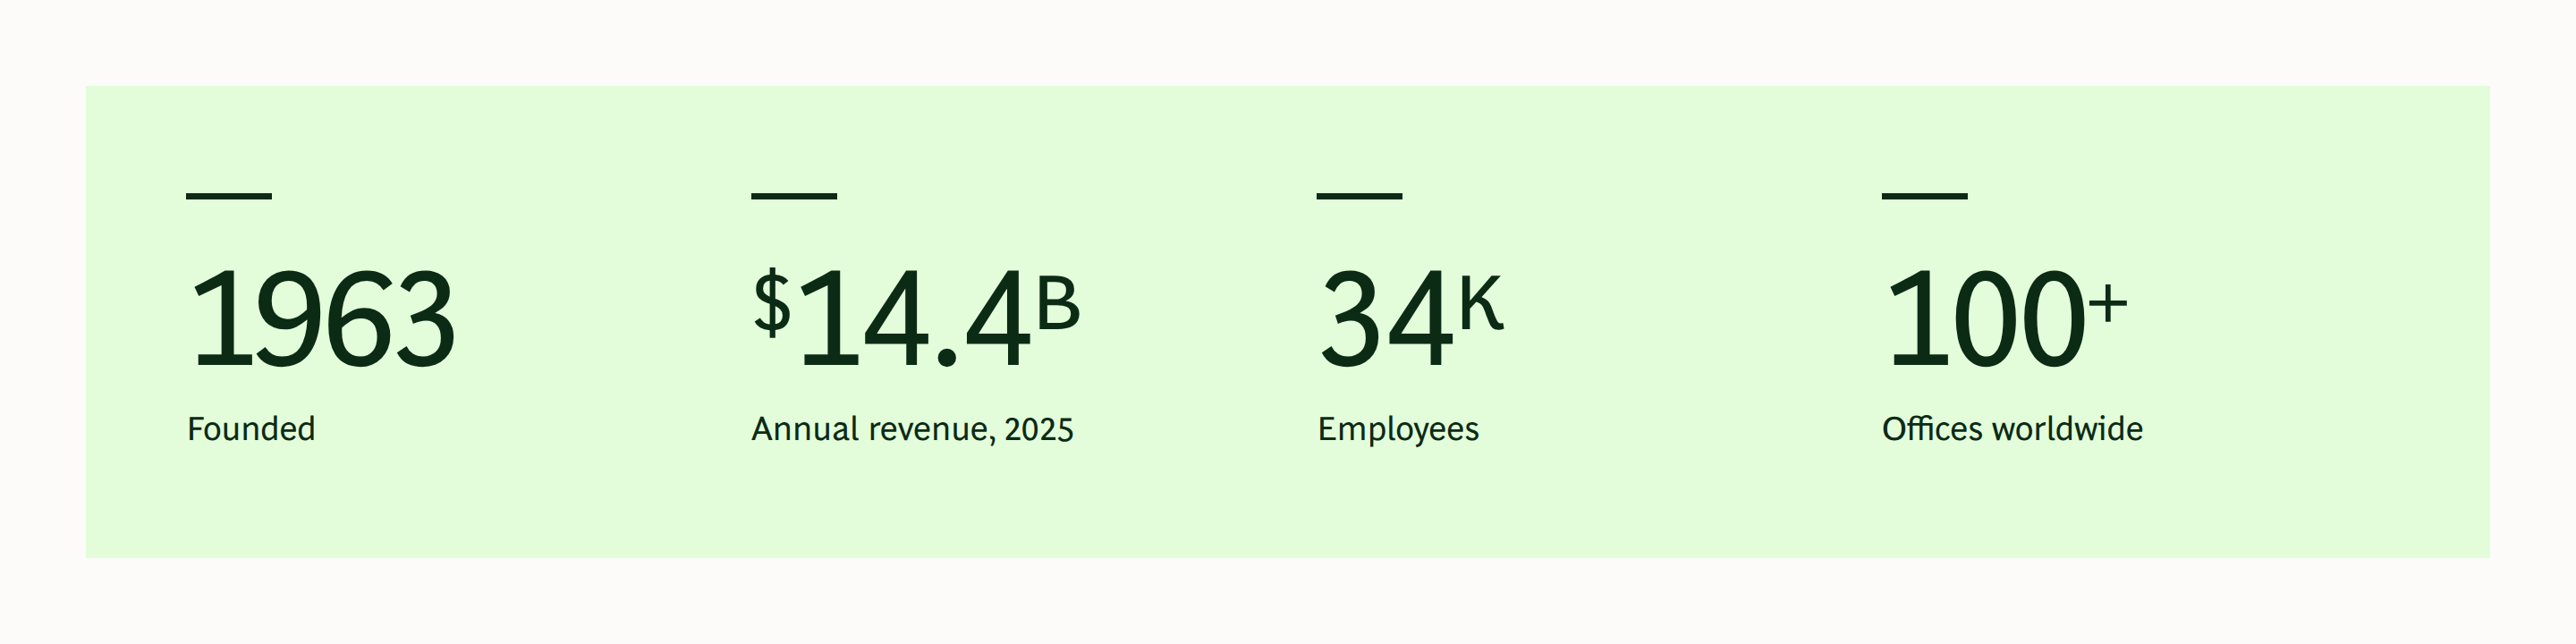
\includegraphics[width=\linewidth]{Figures/bcg-stats-light.png}
  \caption{BCG at a glance (publicly reported figures).}
  \label{fig:bcg-glance}
\end{figure}

\subsubsection{Business areas}

BCG covers business transformation, corporate strategy, digital transformation,
sustainability, mergers and acquisitions, innovation management, and operational
performance. Industry coverage includes healthcare, financial services, consumer
goods, energy, technology, and the public sector.

\subsection{BCG X}

\begin{figure}[H]
  \centering
  
\includegraphics[scale=1]{Logos/BCG_X.jpg}
  \caption{BCG X logo.}
  \label{fig:bcg-x-logo}
\end{figure}

\subsubsection{Presentation}

BCG~X is the technology, design, and build unit of BCG. It accelerates the
digital transformation of large organizations by combining engineering, data,
and design capabilities with the strategic positioning of the firm. Unlike a
traditional software vendor, BCG~X operates within the broader consulting
environment: beyond delivering software, it also helps organizations build
capabilities and adopt new technologies.

\subsubsection{Business areas}

BCG~X concentrates on four core capabilities:

\begin{itemize}
  \item \textbf{AI and Generative AI}: design and delivery of
    artificial-intelligence solutions for business functions, automation, and
    decision support.
  \item \textbf{Customer Experience for Growth}: digital strategies and customer
    journeys oriented toward growth and engagement.
  \item \textbf{Venture and Business Builds}: end-to-end support of new ventures,
    from idea to market.
  \item \textbf{Digital Platform Builds}: secure and scalable digital platforms
    supporting large-scale trans\-for\-ma\-tions.
\end{itemize}

\subsection{Organizational Structure}

BCG adopts a structured yet agile approach, promoting global collaboration
through its technology unit, BCG~X. Led by Sylvain Duranton (Global Leader) and
Jon Ferris (Chief Financial Officer), BCG~X's organizational structure includes
regional and functional leads who oversee specialized areas and regional
centers. This design ensures efficient global coordination and responsiveness to
client needs.

Each regional center (including Morocco, Germany, China, Singapore, and India) is
managed by dedicated leaders who implement localized yet globally aligned
strategies. This structured regional management facilitates effective service
delivery tailored to local market requirements while maintaining consistent
global standards.

\begin{figure}[H]
  \centering
  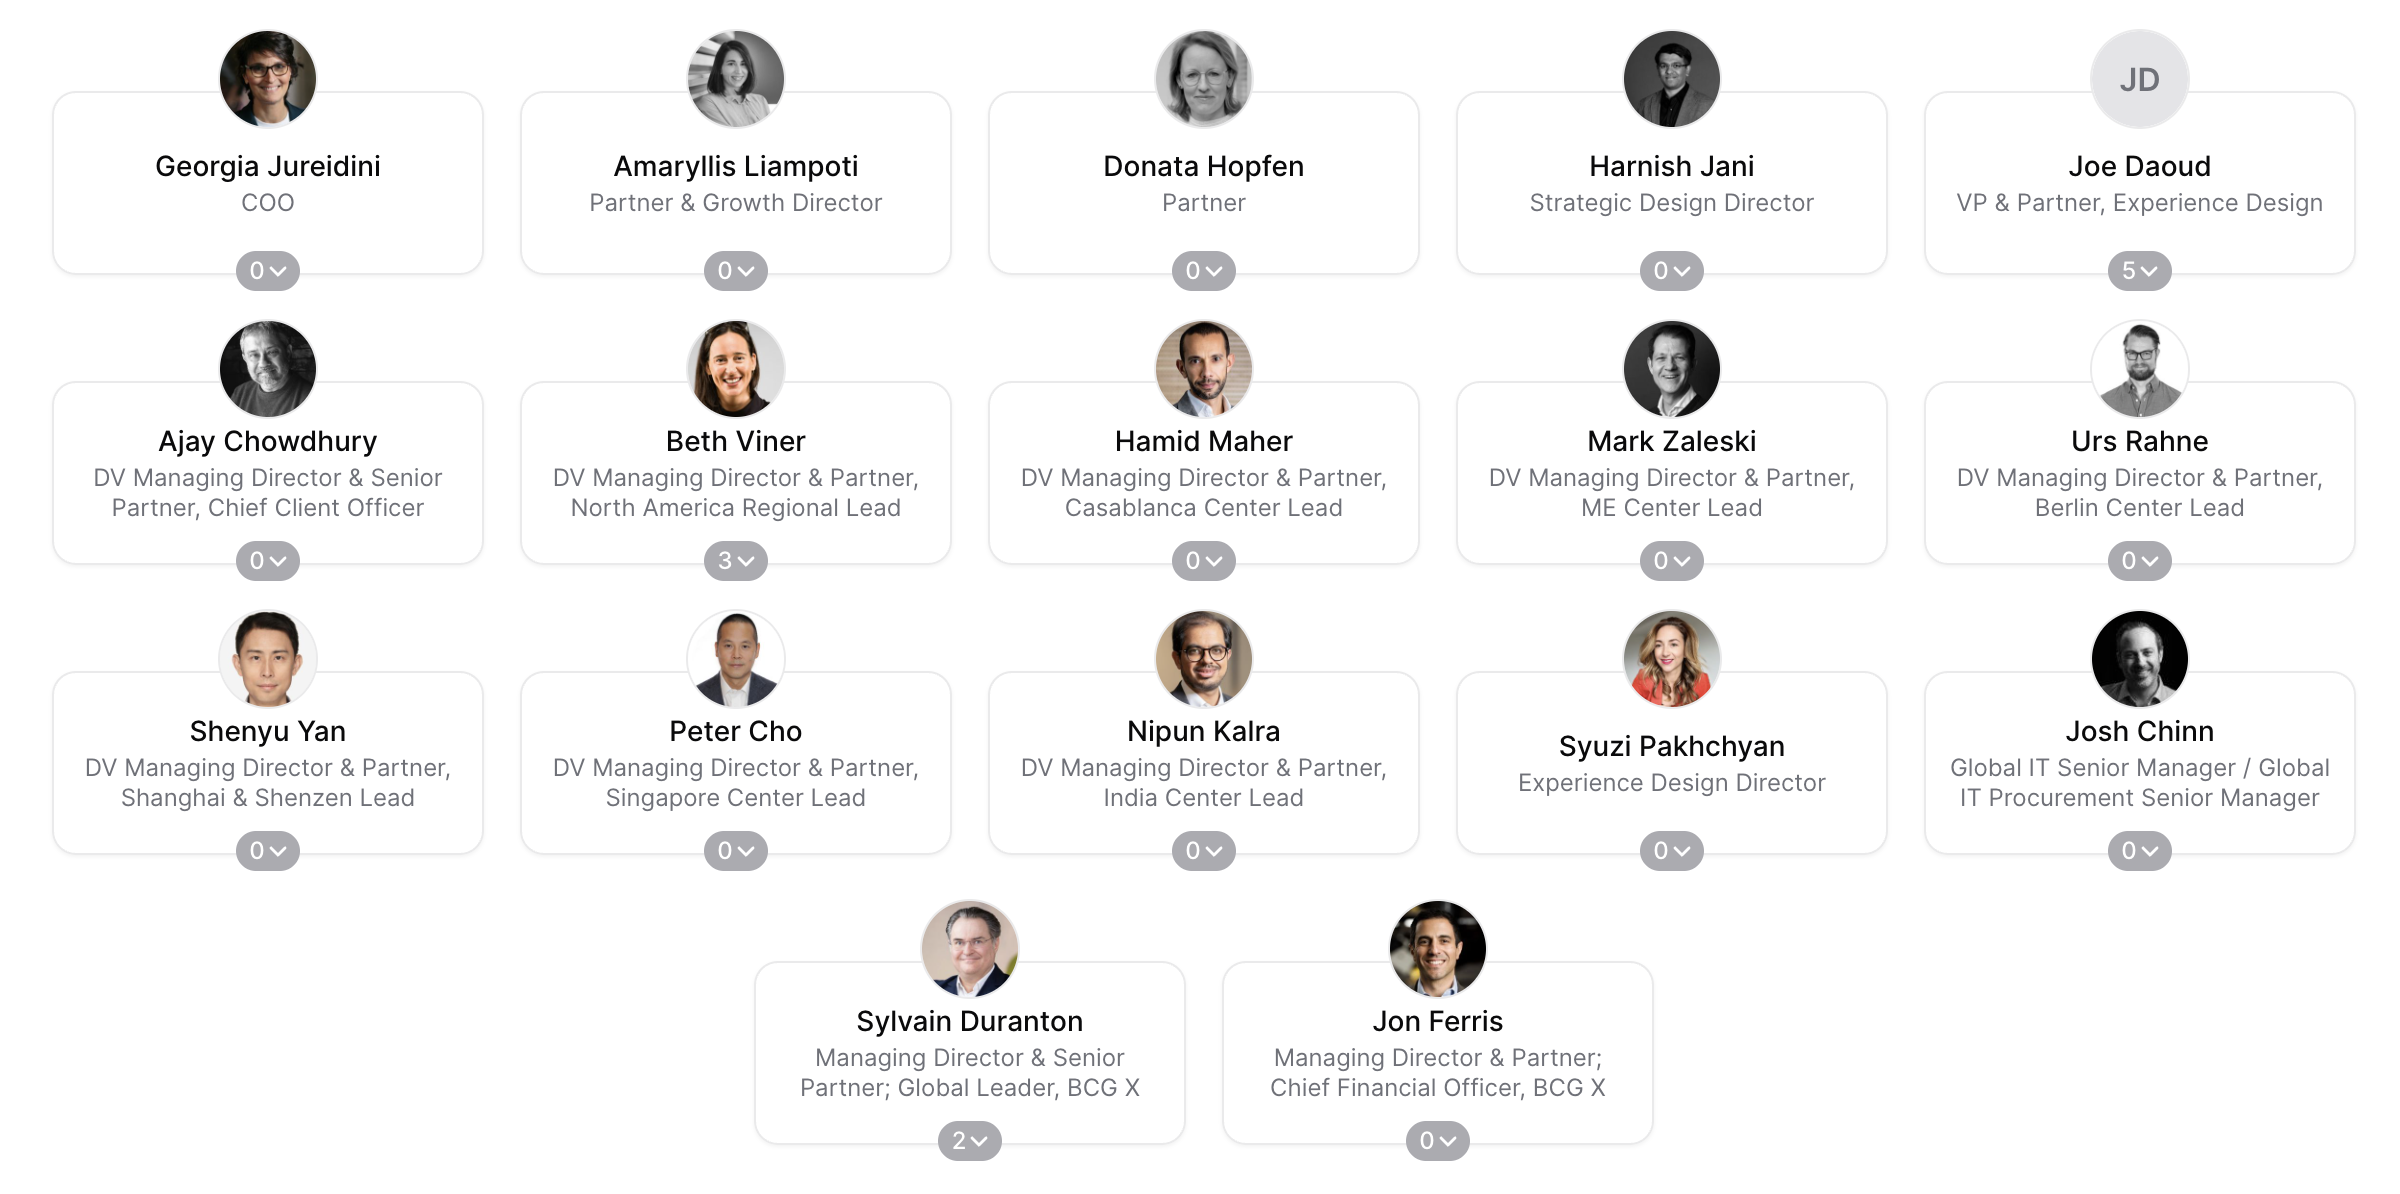
\includegraphics[width=\linewidth]{Figures/executive_leadership_board.png}
  \caption{BCG X leadership and footprint.}
  \label{fig:bcg-x-org}
\end{figure}

\subsection{Organizational Culture}

BCG~X fosters a culture defined by innovation, inclusivity, and entrepreneurial
spirit: team members are encouraged to take on ambiguous, high-impact problems and
to collaborate openly across disciplines and geographies to deliver digital
solutions for clients.

\subsection{The Energy Transition Optimizers team}
\label{sec:team}

The work presented in this report was conducted within the \textbf{Energy
Transition Optimizers} product team of BCG~X, which develops analytical products
dedicated to energy-transition projects, with a particular focus on Power-to-X
evaluation and investment-support workflows. Part of the team operates from the
BCG~X Casablanca center, alongside contributors across other geographies.

Rather than a single tool, the team maintains a small portfolio addressing
different levels of analysis: the \textbf{Energy Transition Optimizer} (the
project-level product concerned by this report), a \textbf{Portfolio Optimizer}
that compares several candidate projects under investment constraints, and a
broader \textbf{Just Energy Transition} tool that evaluates energy-transition
scenarios at a system level. This report focuses on the project-level Energy
Transition Optimizer.

The team combines product ownership, technical leadership, software engineering,
and data-oriented contributions. Figure~\ref{fig:team} summarizes its composition
and the main involvement of each member.

\begin{figure}[H]
  \centering
  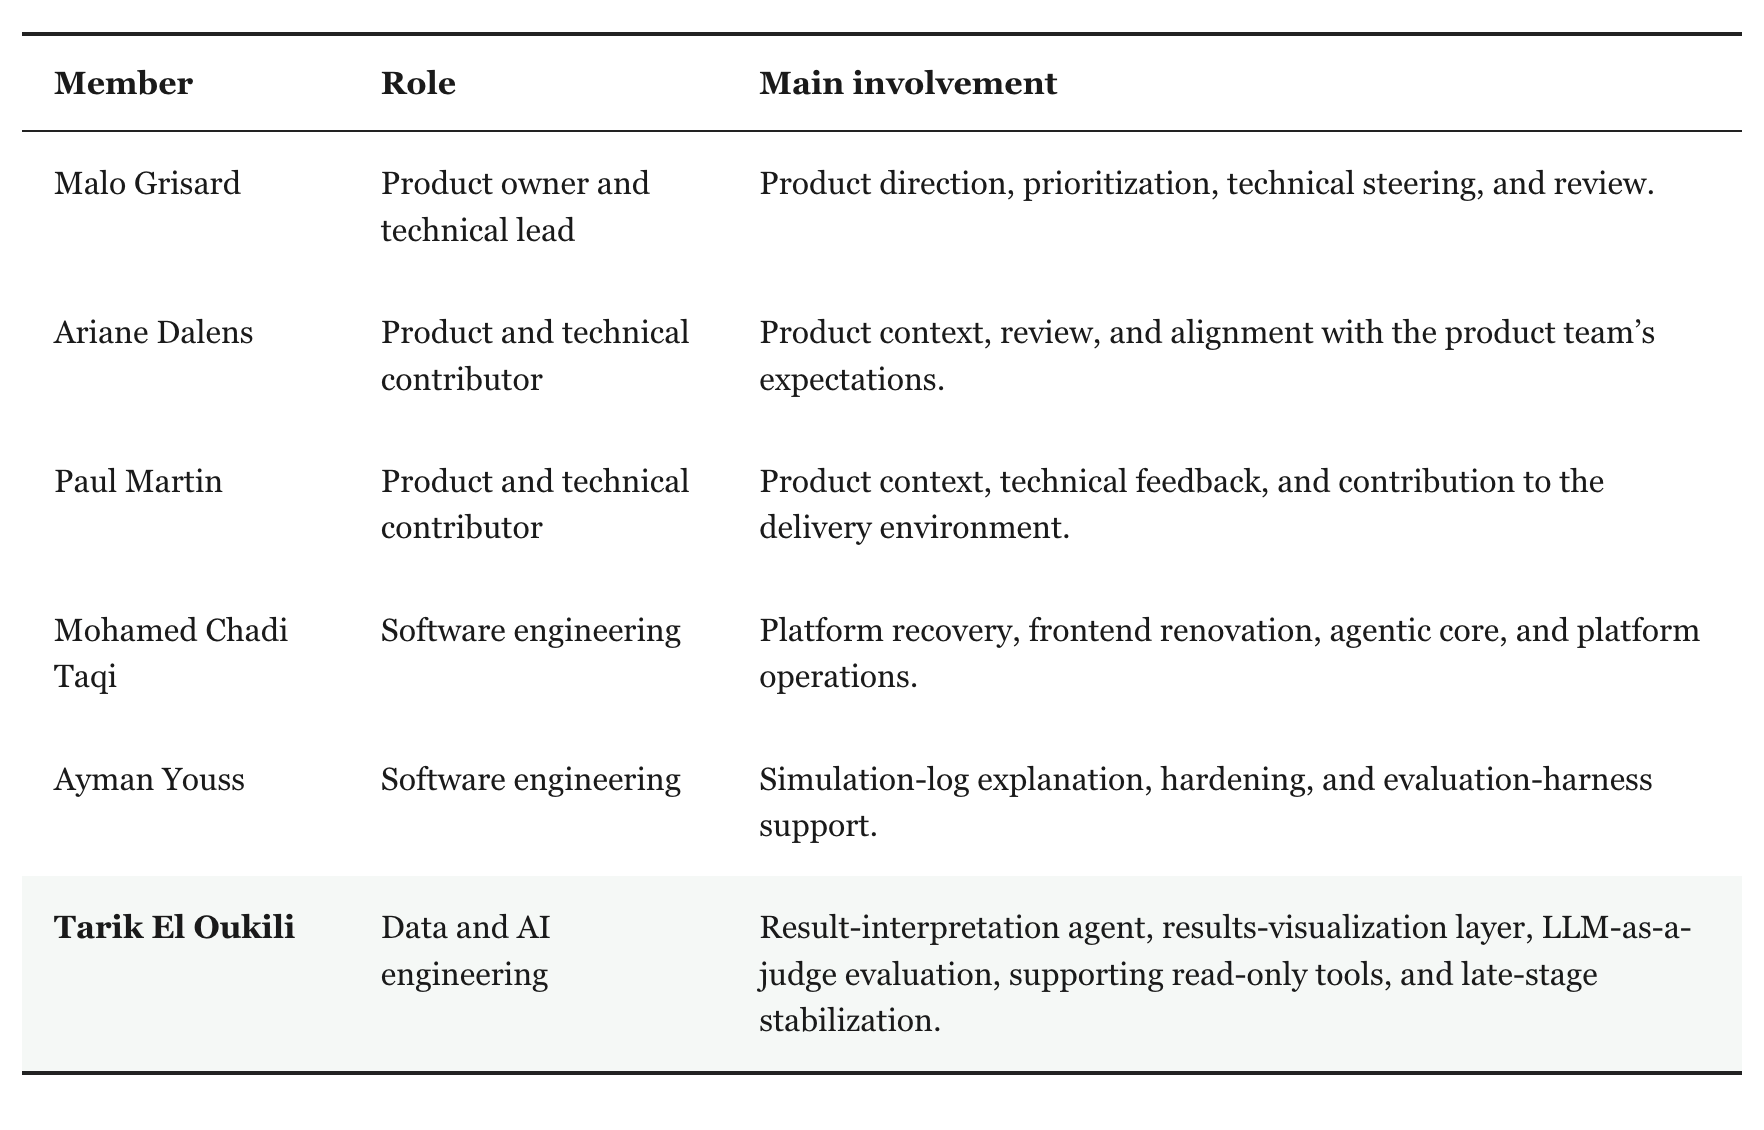
\includegraphics[width=\linewidth]{Figures/team.png}
  \caption{The Energy Transition Optimizers product team and main involvement.}
  \label{fig:team}
\end{figure}

\subsection{Internal products versus client engagements}
\label{sec:internal-product}

BCG~X delivers value through two complementary modes, and the distinction
between them shapes this entire project. In a \textbf{client engagement}, a team
builds a bespoke solution that is scoped, funded, and owned by a single client to
answer that client's specific case; the deliverable is tailored to that client
and is rarely reused as such. In an \textbf{internal product} (sometimes called
an accelerator or asset), BCG~X invests in a reusable capability that is built
and maintained in-house, and then adapted and deployed for several clients on top
of the same core.

The \textbf{Energy Transition Optimizer belongs to the second category}: it is an
internal product, not a one-off client deliverable. Several consequences follow,
and they are referenced throughout this report:

\begin{itemize}
  \item \textbf{Product-level requirements.} Reusability, maintainability,
    reproducibility, and the ability to adapt the same core to different clients
    (hence the several deployment modes described later) take precedence over the
    delivery of a single case.
  \item \textbf{Justified engineering rigor.} Continuous integration, automated
    testing, observability, and data versioning are warranted because the product
    is maintained over time and evolves across client adaptations, rather than
    being discarded at the end of an engagement.
  \item \textbf{A shared capability.} The governed multi-agent layer is designed
    as a product-level capability that lowers the barrier for \emph{every} future
    client adaptation, not as a bespoke feature for one client.
  \item \textbf{Confidentiality.} Because the product is a reusable internal
    asset, the sensitive element is never the product itself but any individual
    client that adopts it, which is the basis of the anonymization stated in
    Section~\ref{sec:confidentiality}.
\end{itemize}


\section{Internship Framework and Confidentiality}
\label{sec:confidentiality}

\begin{quote}
This internship was carried out at BCG~X, the technology and design unit of
Boston Consulting Group. To respect client confidentiality, the identity of the
end client and any customer-, site-, or counterparty-specific data have been
generalized. This anonymization does not alter the methodology, the technical
choices, or the results presented in this report.
\end{quote}

This follows directly from the operating model described in
Section~\ref{sec:internal-product}: the Energy Transition Optimizer is an
internal product rather than a client-specific deliverable. The sensitive element
is therefore never the product itself, which is described in full, but any
individual client that adopts it. Accordingly, the product, its engine, and the
governed agentic layer are presented in detail, while any specific client is
designated only as ``the client''.

\section{Energy Transition and Power-to-X}

\subsection{The decarbonization imperative}

The energy transition refers to the shift from fossil-based energy systems
toward low-carbon and renewable alternatives. While renewable electricity has
expanded rapidly, several sectors, heavy industry, aviation, maritime transport,
and high-temperature industrial processes, remain difficult to decarbonize
through direct electrification alone. For these hard-to-abate sectors,
\textbf{Power-to-X} (PtX) provides alternative energy carriers: renewable
electricity is used, most commonly through water electrolysis, to produce green
hydrogen and its derivatives (ammonia, methanol, and sustainable aviation fuel)
that can be stored, transported, and used where electrons cannot
(Figure~\ref{fig:power-to-x}).

\begin{figure}[H]
  \centering
  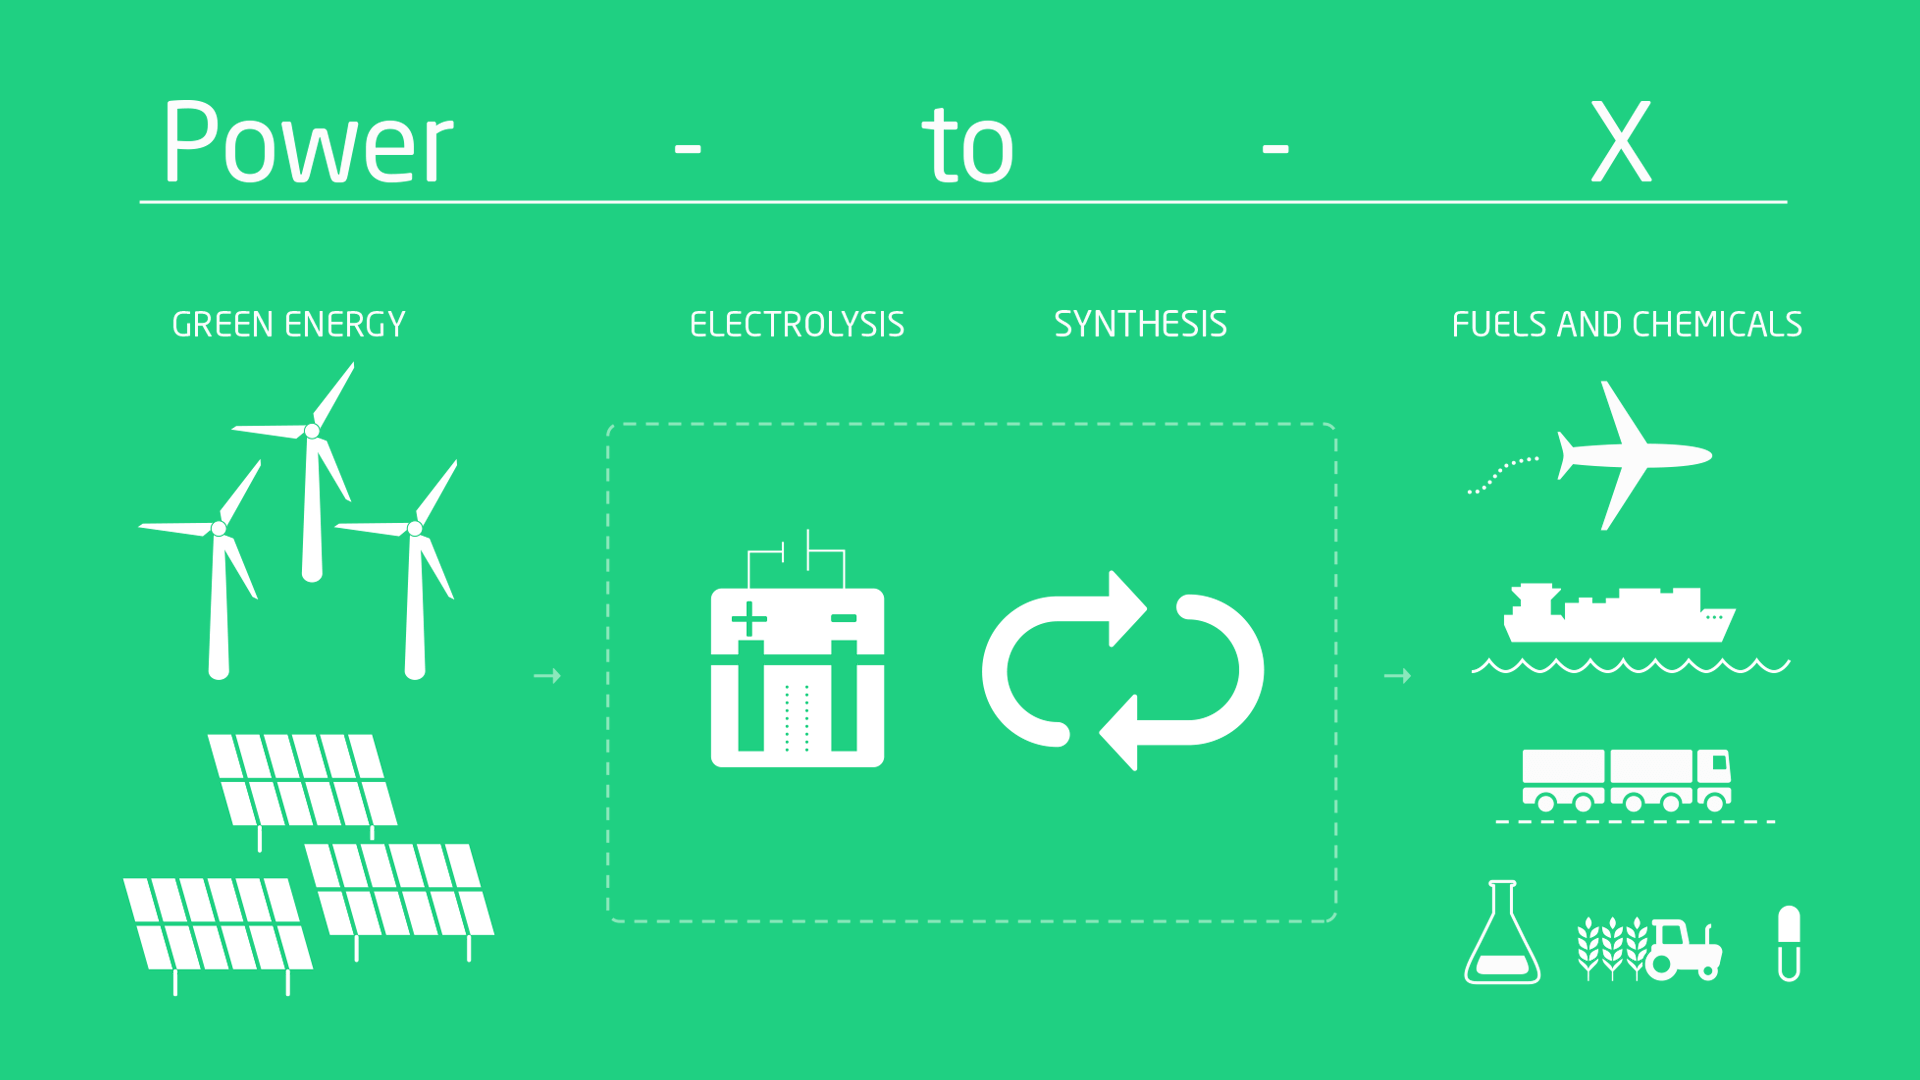
\includegraphics[width=0.8\linewidth]{Figures/power-to-x-technology.png}
  \caption{The Power-to-X principle: renewable electricity converted into
    storable, transportable energy carriers.}
  \label{fig:power-to-x}
\end{figure}



\subsection{Pre-feasibility analysis}

Power-to-X projects are capital-intensive infrastructure projects whose
development requires long planning cycles and coordination between technical,
commercial, financial, and regulatory stakeholders. The \textbf{pre-feasibility}
stage is decisive: sponsors must judge whether a project is promising enough to
justify further engineering and investment, while many assumptions remain
uncertain and cost estimates carry wide accuracy ranges. Pre-feasibility
analysis must therefore provide reliable and explainable results that help
decision-makers compare configurations, estimate economic performance, and
identify the main drivers of value and risk.

\section{The Energy Transition Optimizer}

\subsection{The product and its deterministic core}

To support this process, BCG~X developed the \textbf{Energy Transition
Optimizer} (also referred to internally as the Project Optimizer), a platform
dedicated to the pre-feasibility assessment of individual Power-to-X projects
(Figure~\ref{fig:eto-product}). It
combines a deterministic analytical core with a user-facing application.

In the engine's vocabulary, a project is described by a \textbf{topology}: a
typed directed graph whose nodes are assets (solar, wind, battery, electrolyzer,
converters, storage), commodity-conservation buses, and markets, and whose edges
represent admissible energy or material flows. Together with several hundred
technical and financial parameters (capacity factors, capital and operating
costs, the weighted-average cost of capital, escalation, and tax rates), this
topology is turned into an optimization model that simulates operation
\textbf{hour by hour} over the project's lifetime. A \textbf{grid search} sweeps
ranges of parameters to produce a population of simulations, from which the
engine reports indicators such as net present value (NPV), internal rate of
return (IRR), and the levelized cost of the output product (LCOX). Because the
results may inform investment decisions, the platform must remain reliable,
reproducible, and auditable.

\begin{figure}[H]
  \centering
  
\includegraphics[width=0.5\linewidth]{Figures/eto.png}
  \caption{The Energy Transition Optimizer product.}
  \label{fig:eto-product}
\end{figure}


\subsection{Initial situation}

Before this work began, the Energy Transition Optimizer had reached a fragile
operational state. Its analytical core remained valuable, but the surrounding
product limited its use: the workflow was expert-only, the interface was dated,
and the platform carried delivery and security weaknesses. These limitations,
which are analyzed in detail at the start of Chapter~\ref{chap:background},
motivated the two-level problem stated below.

\section{Problem Statement and Objectives}

\subsection{Problem statement}

The situation defined a two-level problem. At the \textbf{platform level}, the
product needed a restored, secure, and reproducible foundation before it could
be extended safely. At the \textbf{workflow level}, it needed to become
accessible to non-specialists without losing the rigor on which its value
depends. Meanwhile, advances in large language models opened the possibility of
a natural-language interface, but integrating such a capability into an
authoritative analytical engine raises a central tension, which frames the whole
project:

\begin{quote}
\textit{How can generative AI make an expert-only techno-economic optimizer
accessible in natural language, while preserving the reproducibility,
auditability, and human control that its results demand? In other words, how can
the assistant \emph{assist} without becoming the source of numerical truth?}
\end{quote}

\subsection{Scoping questions and expected outcomes}

This tension was broken down into a small set of scoping questions that guided the
work:

\begin{itemize}
  \item Which parts of the pre-feasibility workflow can be delegated to a language
    model, and which must remain under deterministic control?
  \item How can assisted actions be made auditable and reversible, so that a user
    can trust them and, if needed, undo them?
  \item How should the quality of a non-deterministic capability be measured
    rather than assumed?
  \item How can the same capabilities remain maintainable and adaptable across
    several client deployments?
\end{itemize}

The expected outcome was a system in which a non-specialist can design, run, and
interpret a study in natural language, where every state-changing action is
validated and approved, and where the assistant's behavior is continuously
measured, without the deterministic optimizer ever ceding its role as the source
of numerical truth.

\subsection{Objectives}
\label{sec:objectives}

The project was structured around two complementary goals. The first was to
\textbf{consolidate the platform foundation}: restore the delivery pipeline,
remediate security findings, migrate to enterprise identity, correct
infrastructure drift, renovate the interface, and improve observability. The
second was to introduce a \textbf{governed multi-agent conversational layer}: a
director agent that routes each request to specialized agents (data ingestion,
topology design, scenario exploration, and result interpretation), where every
state-changing action remains a typed proposal that is validated and then
subject to explicit human approval, so that the deterministic engine remains the
sole numerical authority.

At the heart of this effort, the agentic layer rests on three pillars,
detailed in the following chapters:

\begin{itemize}
  \item \textbf{The result-interpretation agent}: a read-only sub-agent that
    explains the economics of a simulation population in natural language, with
    every figure traceable back to a deterministic result and no invented
    numbers.
  \item \textbf{The results-visualization layer}: interactive exploration of
    outputs, including interpret-on-demand scatter plots and a navigable
    discounted-cash-flow table.
  \item \textbf{The evaluation harness}: an ``LLM-as-a-judge'' mechanism that
    measures the factual grounding and financial soundness of the explanations
    produced.
\end{itemize}

Methodologically, the work followed the arc of a design-oriented engineering
project rather than a controlled experiment: it identifies the problem and its
constraints (this chapter), reviews the state of the art and chooses a direction
(Chapter~\ref{chap:background}), specifies the requirements
(Chapter~\ref{chap:requirements}), designs and builds the artifacts
(Chapter~\ref{chap:design}), demonstrates them in the delivered product, and
evaluates the assisted behavior against explicit criteria
(Chapter~\ref{chap:implementation}), with the limits of that evaluation stated
rather than hidden. This progression structures the chapters that follow.

\section{Project Management}

\subsection{Agile delivery approach}

The project followed an agile delivery approach adapted to a product-modernization
effort. Rather than fixed sprint boundaries, the work progressed through short
delivery cycles and overlapping thematic phases: the platform foundation was
consolidated first, the governed agentic core was introduced next, specialist
capabilities (including result interpretation) were then extended, and a final
phase focused on observability, hardening, and handover. Priorities were adjusted
as the dependencies between infrastructure, security, and the agentic layer became
clearer, while continuous integration and regular review with the product team
kept the application deployable throughout. My own work followed the same rhythm,
moving from the visualization layer to the interpreter agent and its evaluation,
as shown in the timeline at the end of this section. Within each phase, the work
iterated through the classic agile cycle of requirements, design, development,
testing, deployment, and review (Figure~\ref{fig:agile-cycle}).

\begin{figure}[H]
  \centering
  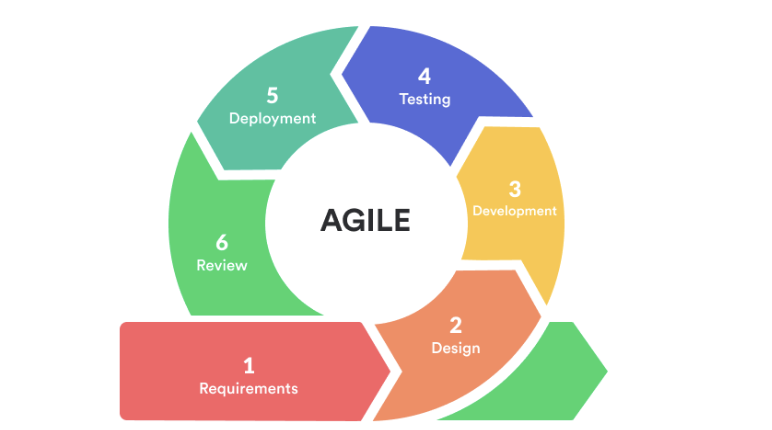
\includegraphics[width=0.62\linewidth]{Figures/agile_cycle.png}
  \caption{The agile delivery cycle followed within each thematic phase.}
  \label{fig:agile-cycle}
\end{figure}

\subsection{Working cadence}

The internship followed the standard cadence of a BCG engagement, built around a
small set of recurring meetings:

\begin{itemize}
  \item \textbf{Daily check-in} in the morning to align on the day's priorities
    and any blockers.
  \item \textbf{Daily check-out} in the afternoon to review progress and hand
    off open items.
  \item \textbf{Case Team Meeting} once a week with the engagement
    Managing Directors and Partners, focused on direction, risks, and key
    decisions.
  \item \textbf{Monthly retrospective} to reflect on what worked, what did not,
    and how to improve.
\end{itemize}
\subsection{Collaboration tools}

The engagement used a small, shared set of tools. Most supported communication
and coordination across the wider team; the technical team additionally used
GitHub, with CircleCI for continuous integration, for code review and delivery.

\begin{itemize}\itemsep=10pt
  \item \textbf{Zoom} and \textbf{Microsoft Teams}: video and audio calls, daily
    check-ins and check-outs, Case Team Meetings, and engagement-wide channels.\\[5pt]
    \mbox{}\hfill
\includegraphics[height=1.9cm]{Logos/zoom.png}\hspace{1.6em}%
    
\includegraphics[height=1.9cm]{Logos/teams.png}\hfill\mbox{}
  \item \textbf{Trello}: a kanban board tracking work items, each card carrying an
    owner, a status, and a short description.\\[5pt]
    \mbox{}\hfill
\includegraphics[height=1.9cm]{Logos/trello.png}\hfill\mbox{}
  \item \textbf{Slack}: lightweight, asynchronous chat within the technical team.\\[5pt]
    \mbox{}\hfill
\includegraphics[height=1.9cm]{Logos/slack.png}\hfill\mbox{}
  \item \textbf{Outlook}: email and calendar management for the recurring
    meetings.\\[5pt]
    \mbox{}\hfill
\includegraphics[height=1.9cm]{Logos/outlook.png}\hfill\mbox{}
  \item \textbf{GitHub}: code hosting and pull-request review, with CircleCI
    running continuous-integration checks on every change.\\[5pt]
    \mbox{}\hfill
\includegraphics[height=1.9cm]{Logos/github.png}\hfill\mbox{}
\end{itemize}

\subsection{Timeline and milestones}

The internship ran from \textbf{June to September 2026}. My work followed the plan
shown in Figure~\ref{fig:gantt}, organized into two overlapping phases that moved
from the results-visualization layer to the interpreter agent and its evaluation.

\textbf{Phase~1 (visualization and financials)} covered the results-visualization
layer: interactive results exploration, chart user-experience and polish, the
drillable discounted-cash-flow (DCF) financials table, and a consolidating
refactor of the visualization and financial components.

\textbf{Phase~2 (interpreter and evaluation)} built the result-interpretation
agent and the means to evaluate it: the interpreter sub-agent, its narration
prompt and grounding rules, Langfuse tracing and datasets, the LLM-as-a-judge
rubrics, a refactor of the agent and evaluation code, and a final feedback loop
and demonstration preparation.

\begin{figure}[H]
  \centering
  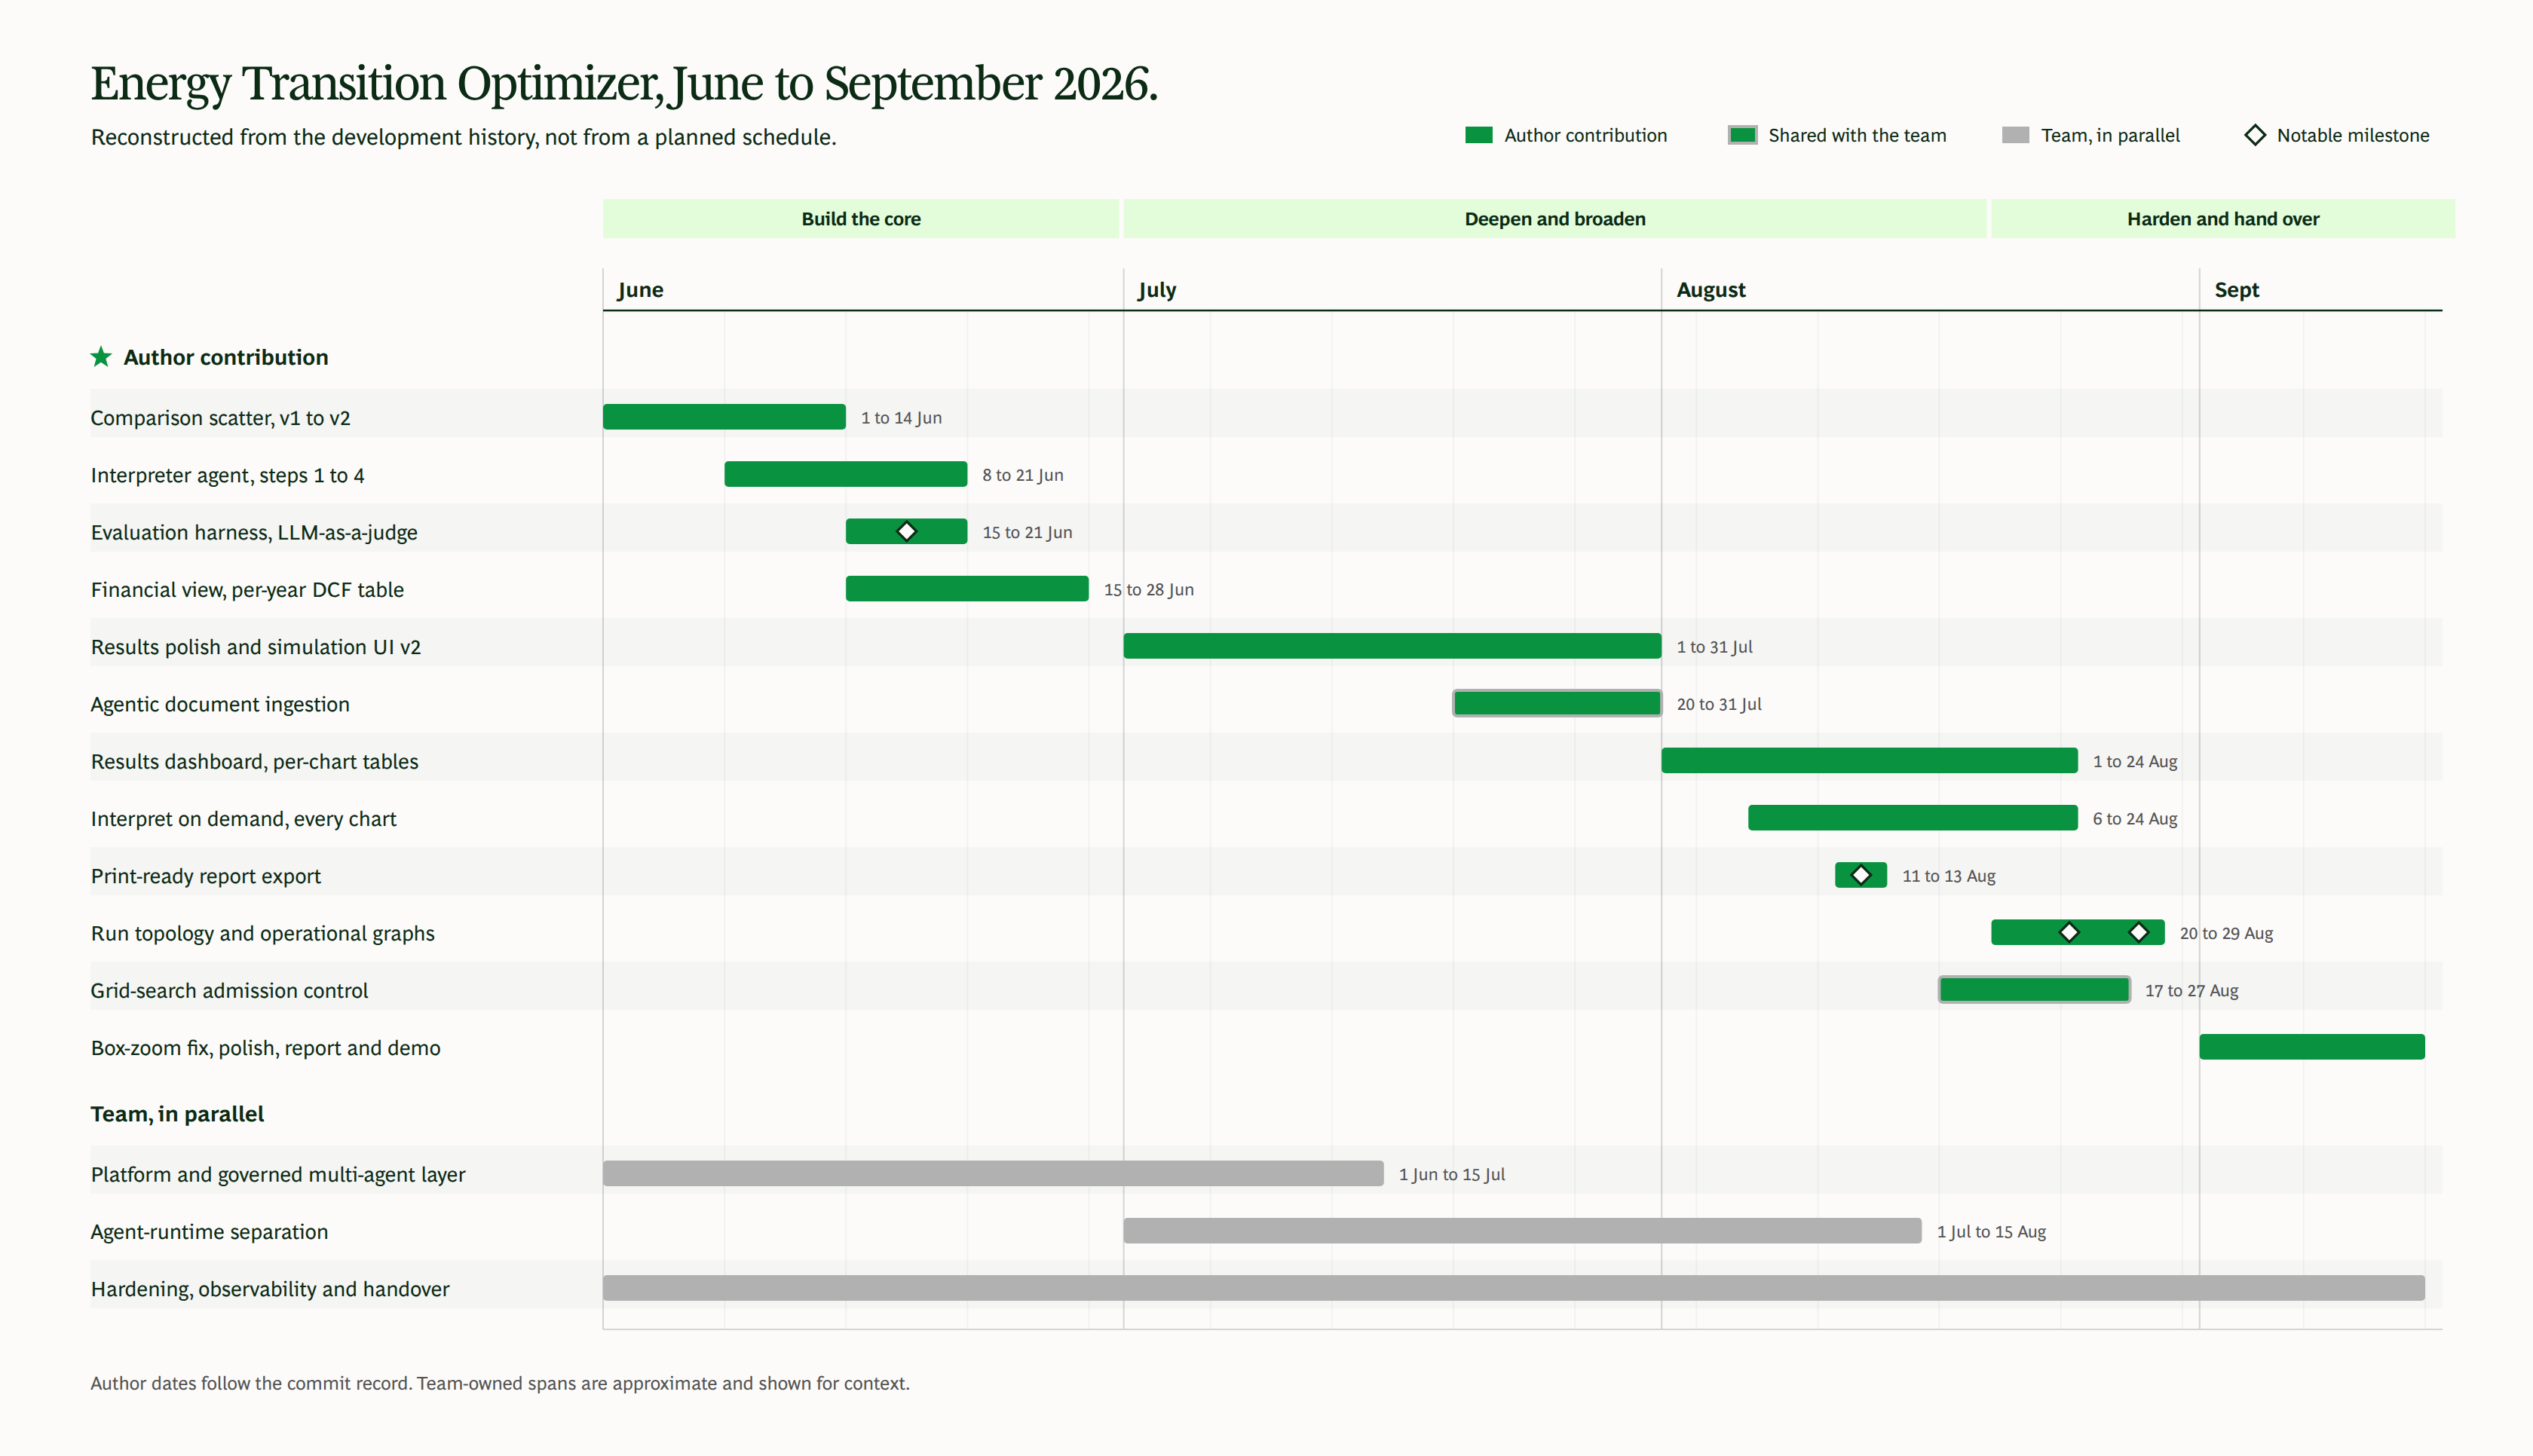
\includegraphics[width=\linewidth]{Figures/optimizer-timeline.png}
  \caption{Internship work plan (June--September 2026).}
  \label{fig:gantt}
\end{figure}

\section*{Conclusion}

This chapter introduced the host organization, the Energy Transition Optimizers
product team, and the energy-transition context of the project. It presented the
Energy Transition Optimizer, its fragile initial state, and the two-level problem
the internship addressed, and it framed the central tension between accessibility
and numerical authority. The next chapter reviews the technical background and
state of the art on which the work rests.


\chapter{State of the Art and Technical Foundations}
\label{chap:background}

\section*{Introduction}

This chapter establishes the technical background on which the rest of the
report rests. The Energy Transition Optimizer is not only a Power-to-X model: it
is an analytical product that must be usable, maintainable, secure, and, with the
new conversational layer, assisted by language models without losing its
numerical authority. For this reason the state of the art is examined along
several axes rather than a single one.

The chapter is organized in four movements. It first studies the existing
platform as the concrete starting point of the project. It then lays the
technical foundations axis by axis, from techno-economic optimization to
language-model agents, and gives particular attention to two axes central to
this work: the interpretation and visualization of
results, and the evaluation of language-model behavior. It then benchmarks the
possible directions and justifies the one adopted. Finally, it positions the
work within that landscape.

\section{Analysis of the existing ETO platform}
\label{sec:existing}

The project did not start from a blank page. The existing Energy Transition
Optimizer already offered a working foundation for Power-to-X pre-feasibility
analysis: users could create projects, define assumptions, build a topology, run
simulations, and inspect numerical outputs. Studying it was essential, because it
made it possible to distinguish what had to be preserved from what had to be
redesigned.



\subsection{A valuable deterministic core}

The analytical core was, and remains, the most valuable part of the product. It
turns a declared topology and a set of assumptions into reproducible operating
schedules and financial indicators. This determinism is precisely what makes the
tool trustworthy for investment-oriented analysis: given the same inputs, it
returns the same result. Any evolution of the product therefore had to protect
this core rather than replace it.

\subsection{An expert-oriented workflow}

The workflow around the core, however, showed the limits of an internal,
expert-only tool. To obtain an answer, a user had to hand-build a valid topology,
bind library assumptions to each node, set sweep ranges across many parameters,
launch a grid search, and finally read a population of results. Each of these
steps assumed prior knowledge of the model and of the meaning of its parameters
(Figure~\ref{fig:experts}).
The tool was powerful for specialists but difficult to approach for the broader
set of analysts who could benefit from it.
\begin{figure}[H]
  \centering
  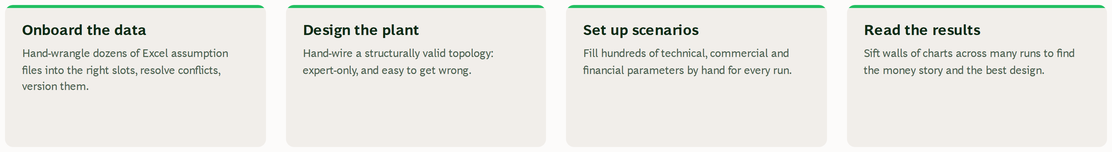
\includegraphics[width=\linewidth]{Figures/plant-workflow-bcg-style.png}
  \caption{An expert-only workflow: a bottleneck on every project.}
  \label{fig:experts}
\end{figure}

\subsection{Dated user experience and unsupported interpretation}

Two weaknesses were especially relevant to this work. First, the visual design
was dated and inconsistent across screens
(Figure~\ref{fig:existing-eto-platform}), which lowered the perceived maturity
of the product and eroded confidence during first use. Second, and more
importantly, \textbf{result interpretation was almost entirely unsupported}. The
platform could display a point on a chart or the status of a simulation, but it
did not explain whether a result was expected, which assumptions had driven it,
or what a user should do next. Turning a table of net present values and internal
rates of return into an operational and financial narrative was left entirely to
the user. This gap is the direct motivation for the interpretation and
visualization work presented later in this report.
\begin{figure}[H]
  \centering
  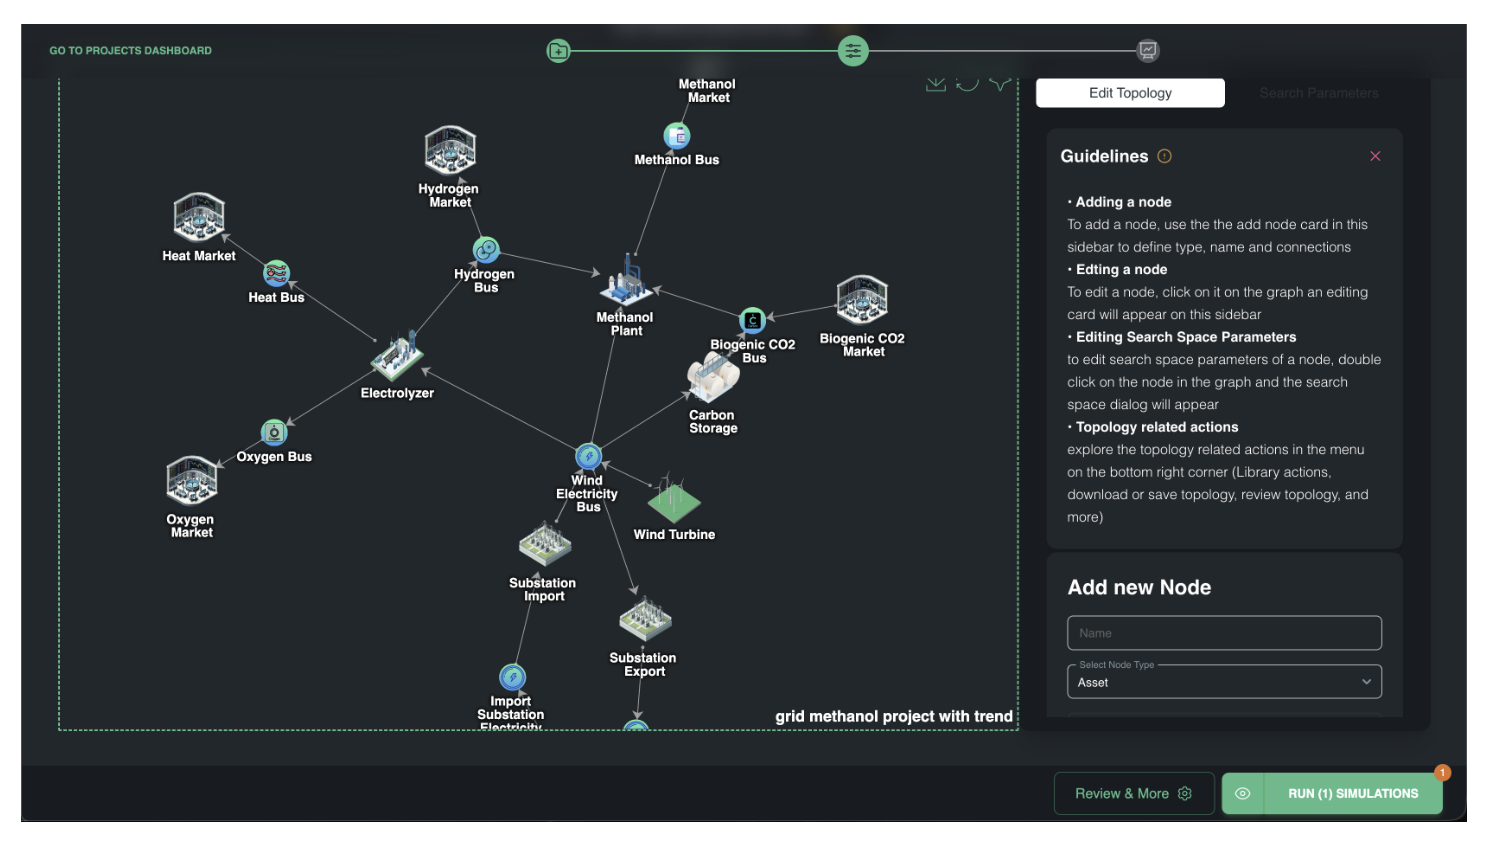
\includegraphics[width=0.48\linewidth]{Figures/old 1.png}
  \hfill
  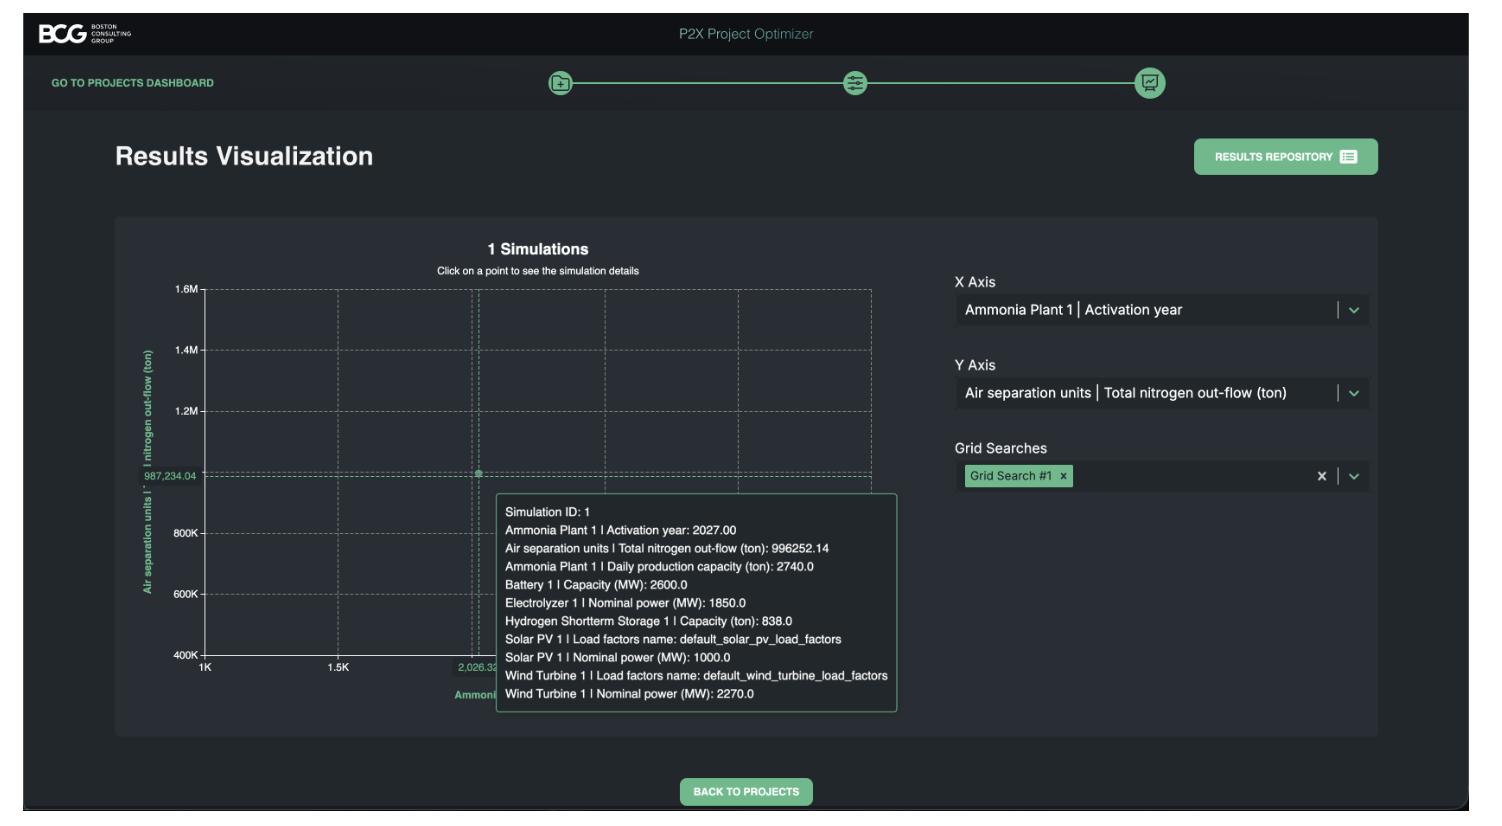
\includegraphics[width=0.48\linewidth]{Figures/old 2.png}
  \caption{Two screens of the existing Energy Transition Optimizer interface.}
  \label{fig:existing-eto-platform}
\end{figure}

\subsection{A fragile platform and inherited identity risk}

Beyond the analytical experience, the product sat on a fragile platform: an
unreliable release process, environments that had drifted from any documented
baseline, and limited operational observability. In parallel, the inherited
authentication layer relied on self-hosted identity components, which placed
identity-provider responsibilities (patching, configuration, monitoring) inside
the application stack and constituted a security and compliance risk in its own
right. These issues had to be addressed before the product could be safely
extended.

\subsection{Synthesis of limitations}

The study of the existing platform can be summarized as follows. The limitations
were not concentrated in one component; they appeared across the user journey:

\begin{itemize}
  \item the workflow was expert-oriented and required prior knowledge of the
    model;
  \item the visual design was dated and reduced confidence during first use;
  \item results were available but their interpretation was mostly unsupported;
  \item the platform lacked any assistance connecting user intent, model
    configuration, execution, and result analysis;
  \item authentication and deployment foundations required modernization before
    the product could scale safely.
\end{itemize}

The key observation is that the missing piece was not the solver, which was
sound, but the product surrounding it. This framing guides the rest of the
chapter and the direction ultimately chosen.

\section{Techno-economic optimization and Power-to-X modeling}
\label{sec:opt-foundations}

\subsection{Linear and mixed-integer programming}

The analytical core belongs to the family of solver-backed optimization tools.
\textbf{Linear programming} (LP) optimizes a linear objective subject to linear
constraints over continuous variables, and is solvable efficiently
\cite{bertsimas1997}. \textbf{Mixed-integer linear programming} (MILP) extends it
with integer or binary variables, which are required whenever discrete operating
states must be represented (for example a unit being on or off)
\cite{nemhauser1988}. Energy-system operation is naturally expressed in this
form: continuous variables carry flows, powers, and inventories, while binary
variables carry discrete commitment decisions, an approach that mirrors classical
unit-commitment modeling in power systems \cite{wood2013, morales2013}. MILP is
NP-hard in general, but modern branch-and-cut solvers make realistic instances
tractable.

\subsection{Multi-carrier energy systems and energy hubs}

A Power-to-X project couples several energy carriers and commodities:
electricity, hydrogen, heat, and downstream molecules such as ammonia or
methanol. Such systems are naturally described as \textbf{multi-carrier energy
systems}, or \emph{energy hubs}, in which conversion and storage units link
inputs and outputs across carriers \cite{geidl2007opf, geidl2007hub}. This is
exactly the abstraction used by the Energy Transition Optimizer, where a project
is a typed graph of assets, commodity-conservation buses, and markets. The
economic and climate relevance of these pathways for hard-to-abate sectors is
well documented \cite{ueckerdt2021, hermesmann2021}.

\begin{figure}[H]
  \centering
  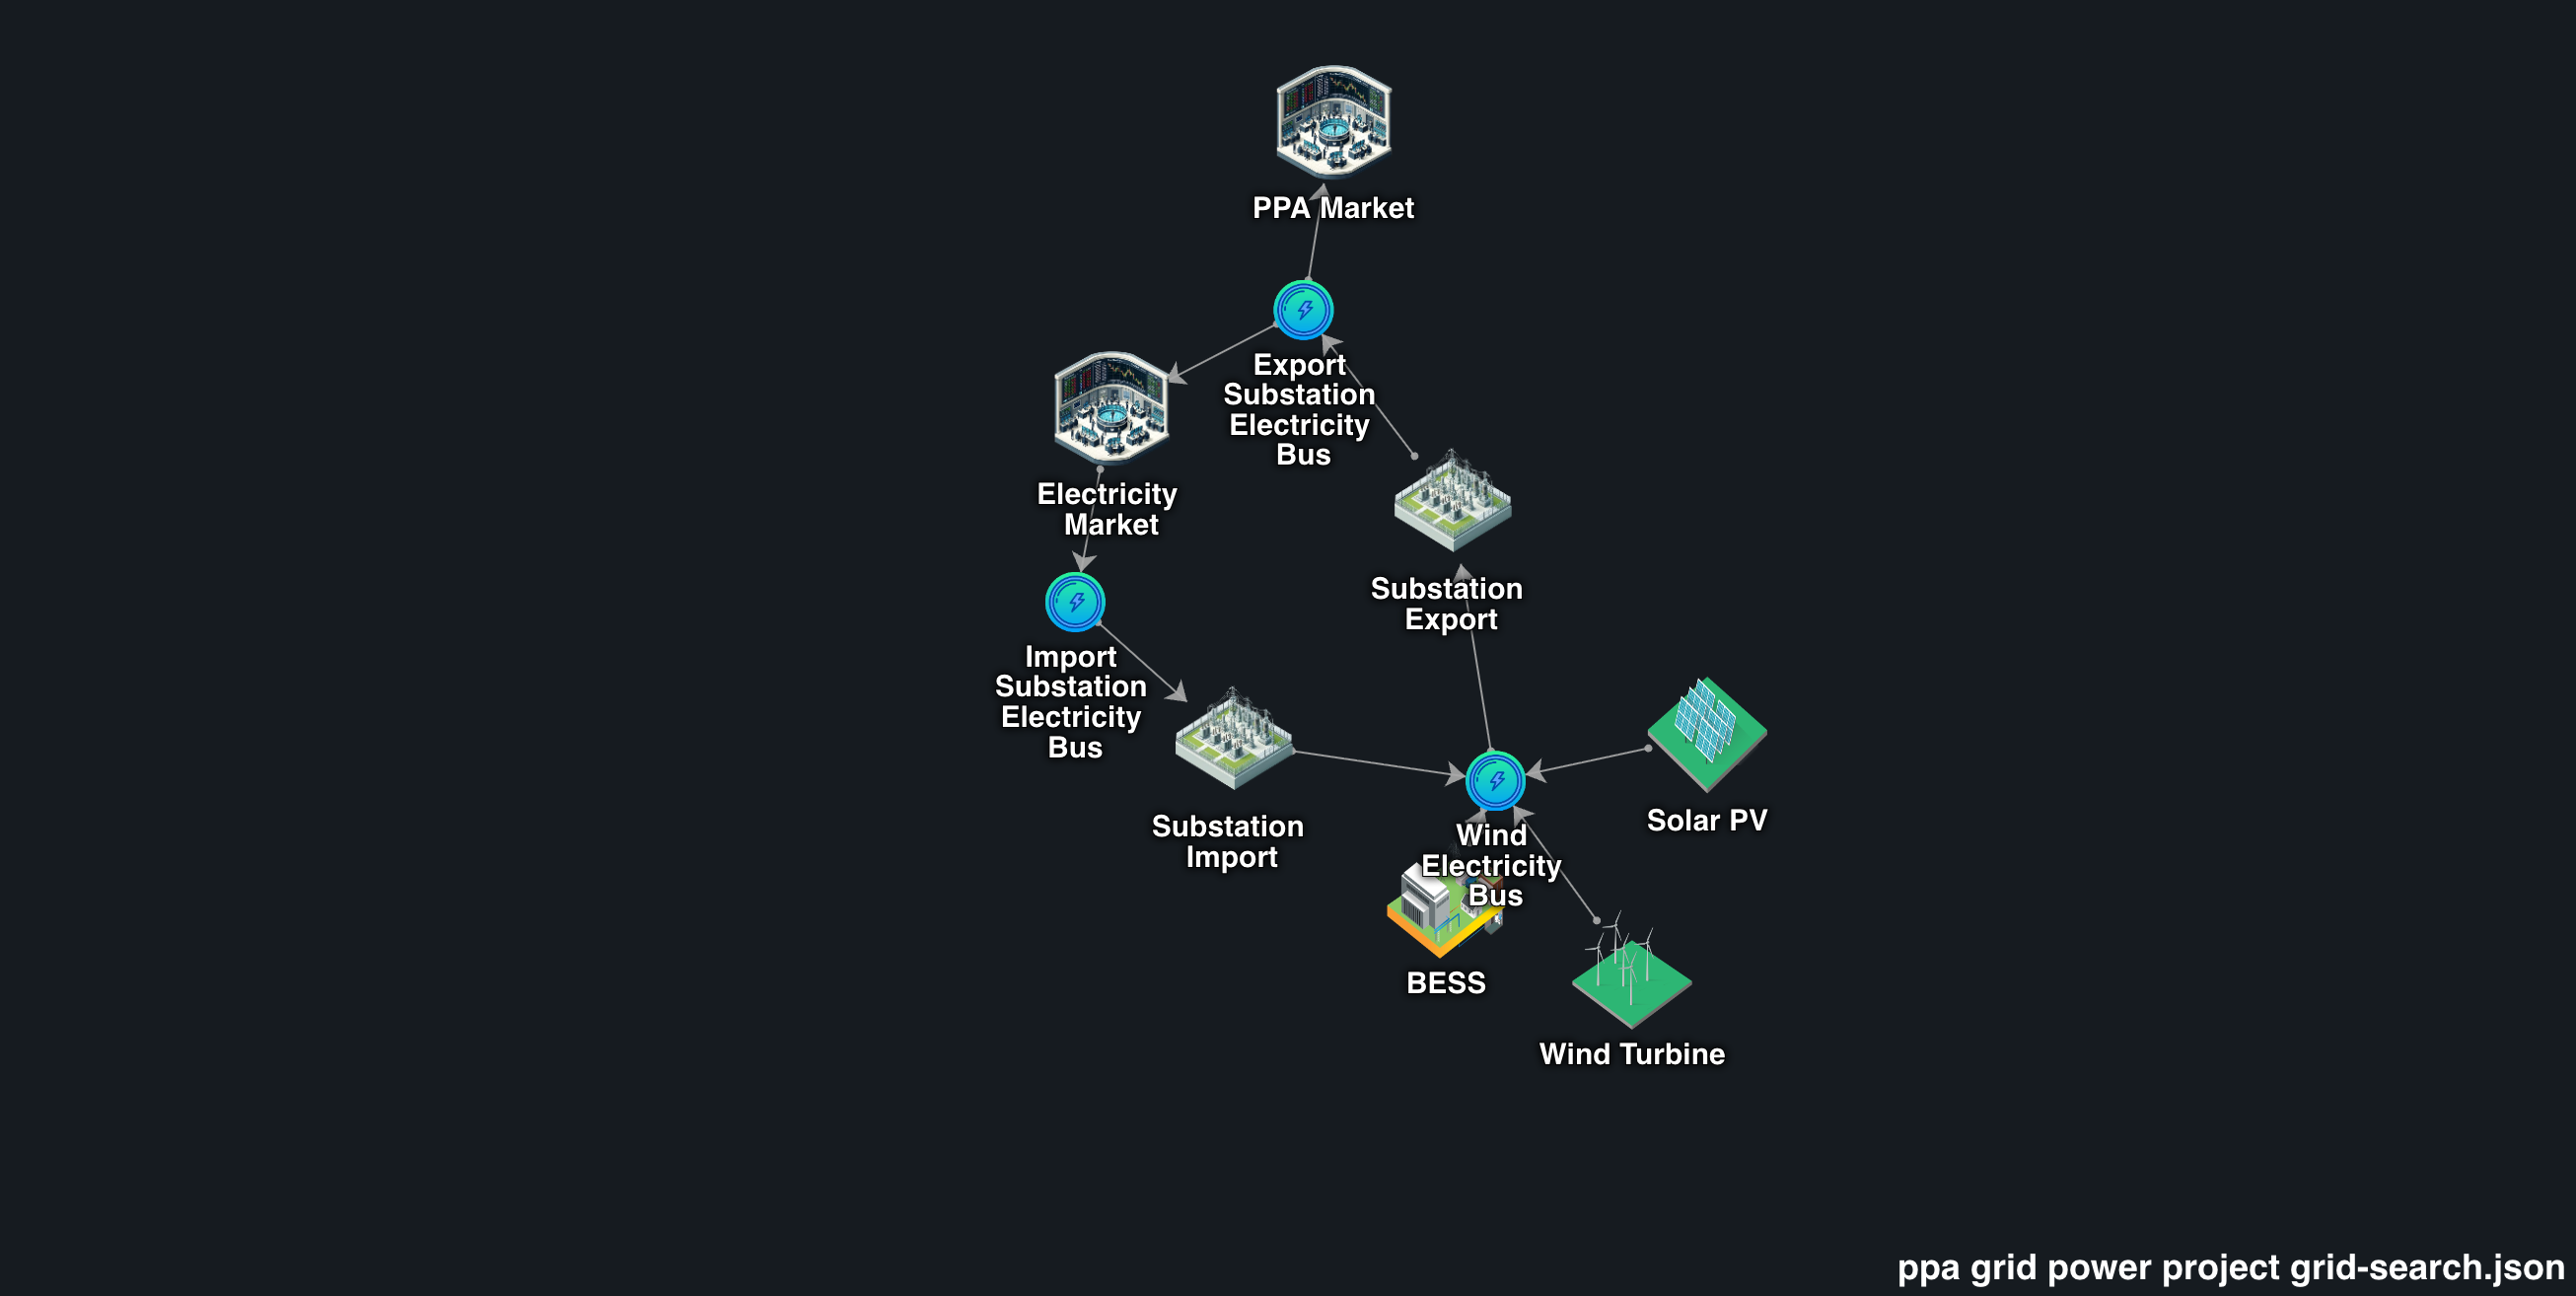
\includegraphics[width=0.8\linewidth]{Figures/energy_hub_example.png}
  \caption{An example multi-carrier topology (energy hub).}
  \label{fig:energy-hub-example}
\end{figure}

\newpage
Figure~\ref{fig:energy-hub-example} shows an example of such a topology.
Concretely, the operational problem solved over each planning window has the
general form of a (mixed-integer) linear program:
\begin{align}
  \min_{x,\,s,\,u}\quad & \sum_{t\in\mathcal{T}} c_t^{\top} x_t \\
  \text{s.t.}\quad
  & \sum_{a\in\mathcal{A}(b)} \sigma_{a,b}\, x_{a,t} = d_{b,t}
    && \forall\, b\in\mathcal{B},\ t\in\mathcal{T} \quad\text{(commodity balance)} \\
  & 0 \le x_{a,t} \le \bar{P}_a
    && \forall\, a\in\mathcal{A},\ t \quad\text{(capacity)} \\
  & x_{a,t} \le \bar{P}_a\, u_{a,t},\quad u_{a,t}\in\{0,1\}
    && \forall\, a\in\mathcal{U},\ t \quad\text{(commitment)} \\
  & s_{a,t} = s_{a,t-1} + \Big(\eta^{c}_a\, x^{c}_{a,t} - \tfrac{1}{\eta^{d}_a}\, x^{d}_{a,t}\Big)\Delta t,\ \ 0\le s_{a,t}\le \bar{S}_a
    && \forall\, a\in\mathcal{S},\ t \quad\text{(storage)} \\
  & s_{a,0} = s^{\mathrm{init}}_a
    && \forall\, a\in\mathcal{S} \quad\text{(initial state)}
\end{align}
where $\mathcal{T}$ indexes the time steps, $\mathcal{B}$ the commodity buses,
$\mathcal{A}$ the assets, $\mathcal{A}(b)\subseteq\mathcal{A}$ the assets incident to
bus $b$, $\mathcal{S}\subseteq\mathcal{A}$ the storage assets, and
$\mathcal{U}\subseteq\mathcal{A}$ the committable assets. The continuous variables
$x$ collect flows and powers, $x^{c}$ and $x^{d}$ the charge and discharge of
storage, and $s$ the storage states of charge, while $u$ are the binary commitment
variables. The data are the signed incidence $\sigma_{a,b}\in\{-1,+1\}$ (production
into a bus positive, consumption negative), the time-varying prices and operating
costs $c_t$, the charge and discharge efficiencies $\eta^{c},\eta^{d}$, the power and
storage capacities $\bar{P}$ and $\bar{S}$, the initial states of charge
$s^{\mathrm{init}}$, and the step duration $\Delta t$. The balance rows express
signed conservation at every bus (the energy-hub abstraction), while the binary
commitment variables make the program mixed-integer. Within a single operational
solve the capacities $\bar{P}_a$ and $\bar{S}_a$ are fixed inputs; the surrounding
grid search varies them across runs, and the resulting cash flows feed the financial
indicators. This is a representative structure of the class, which the engine
elaborates with each project's specific assets, markets, and financial terms.

\subsection{Rolling-horizon operation}

Simulating a project hour by hour over its entire lifetime produces an
optimization problem too large to solve in a single pass. A common remedy is the
\textbf{rolling-horizon} strategy: the long horizon is decomposed into
overlapping shorter windows, each solved in turn, with only the earliest portion
committed and the remainder used as lookahead
(Figure~\ref{fig:rolling-horizon}) \cite{wood2013}. This keeps each
sub-problem tractable while maintaining a coherent trajectory across the full
period, at the cost of trading global optimality for computational feasibility.

\begin{figure}[H]
  \centering
  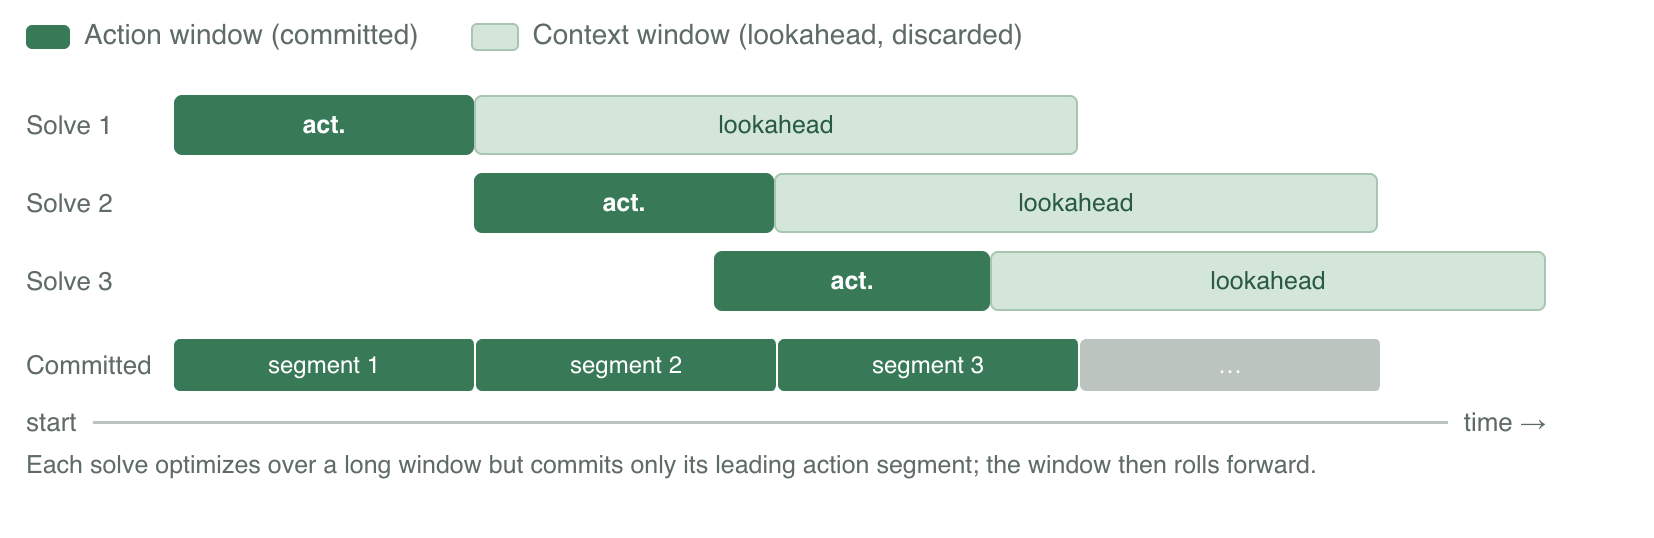
\includegraphics[width=\linewidth]{Figures/rolling_horizon.png}
  \caption{Rolling-horizon decomposition into overlapping windows.}
  \label{fig:rolling-horizon}
\end{figure}

\subsection{Financial indicators for pre-feasibility}

Pre-feasibility analysis translates operating schedules into economic terms. The
core indicators are the \textbf{net present value} (NPV), the \textbf{internal
rate of return} (IRR), and the \textbf{levelized cost} of the output product
(LCOX), all discounted at a \textbf{weighted-average cost of capital} (WACC) and
supported by a full \textbf{discounted-cash-flow} (DCF) statement
(Table~\ref{tab:financial-indicators}). Because
early-stage estimates carry wide accuracy ranges, industry practice formalizes
estimate maturity through cost-estimate classification \cite{aace2020}, and cost
trajectories for renewable generation are tracked by public sources
\cite{irena2023}. These indicators are the raw material that the interpretation
agent must later explain in plain language.

\begin{table}[H]
  \centering
  \small
  \begin{tabularx}{\linewidth}{@{}>{\raggedright\arraybackslash}p{3.9cm} >{\raggedright\arraybackslash}X >{\raggedright\arraybackslash}X@{}}
    \toprule
    \textbf{Indicator} & \textbf{What it measures} & \textbf{Role in pre-feasibility} \\
    \midrule
    Net present value (NPV) & The project's cash flows over its life, discounted to
      today. & Absolute value created; a positive NPV means the project earns above
      its cost of capital. \\
    \addlinespace
    Internal rate of return (IRR) & The discount rate at which the NPV is zero. & A
      single rate to compare against the hurdle rate. \\
    \addlinespace
    Levelized cost of output (LCOX) & Discounted lifetime cost per unit of product
      (hydrogen, ammonia, and so on). & Cost competitiveness of the molecule against
      a benchmark price. \\
    \addlinespace
    Weighted-average cost of capital (WACC) & The blended required return on debt and
      equity. & The rate at which future cash flows are discounted. \\
    \addlinespace
    Discounted cash flow (DCF) & Year-by-year revenue, cost, tax, and net and
      cumulative cash flow, discounted. & The full statement the other indicators
      summarize. \\
    \addlinespace
    Payback period & The time for cumulative discounted cash flow to turn positive. &
      How long invested capital is at risk. \\
    \bottomrule
  \end{tabularx}
  \caption{Financial indicators used in Power-to-X pre-feasibility analysis.}
  \label{tab:financial-indicators}
\end{table}

\subsection{Open frameworks and solvers}

The approach is aligned with a wider movement toward transparent and reproducible
energy-system modeling, exemplified by open frameworks such as \emph{oemof}
\cite{oemof2018} and by calls for openness in the field \cite{pfenninger2018}.
On the solver side, the model can be dispatched through a solver-agnostic
interface such as OR-Tools \cite{ortools} to open-source back ends like the
HiGHS simplex solver \cite{highs2018}, while commercial solvers such as Gurobi
\cite{gurobi2024} remain available for larger instances.

\section{Large language models and agentic systems}
\label{sec:llm-foundations}

\subsection{From language models to reasoning with tools}

Modern large language models (LLMs) are based on the transformer architecture
\cite{vaswani2017} and exhibit strong in-context learning: they adapt to a task
from instructions and examples supplied in the prompt, without retraining.
Prompting techniques such as \textbf{chain-of-thought} improve multi-step
reasoning by eliciting intermediate steps \cite{wei2022cot}. Crucially for this
work, LLMs can be connected to external tools: the \textbf{ReAct} pattern
interleaves reasoning with tool calls so that a model can gather evidence before
answering \cite{yao2023react}, and models can learn to invoke tools with
structured arguments \cite{schick2023toolformer}. This is the mechanism by which
a language model can read facts from a deterministic system rather than inventing
them (Figure~\ref{fig:react-loop}).

\begin{figure}[H]
  \centering
  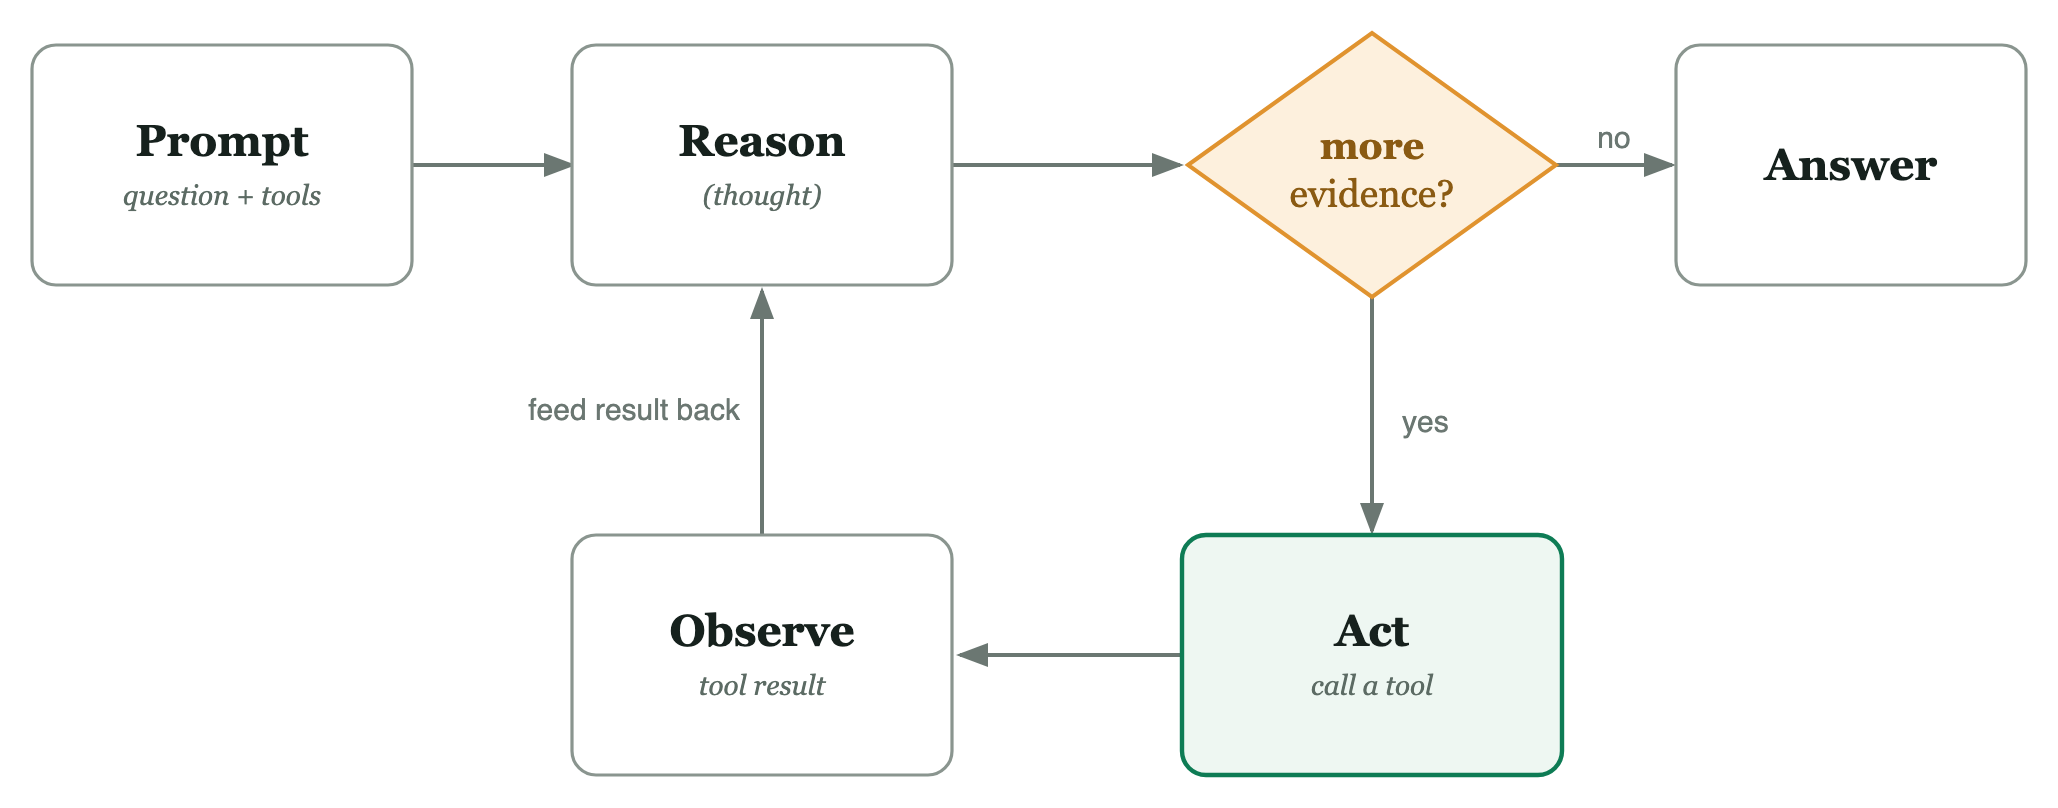
\includegraphics[width=\linewidth]{Figures/react_loop.png}
  \caption{The ReAct pattern: reasoning interleaved with tool calls.}
  \label{fig:react-loop}
\end{figure}

\subsection{Multi-agent orchestration}

Rather than a single monolithic prompt, complex workflows are increasingly built
as \textbf{multi-agent systems}, in which a coordinating agent routes work to
specialized agents, each with a narrow competence and a small tool surface
\cite{wu2024autogen, wang2024survey}. Interoperability between models and tools
is being standardized through protocols such as the \textbf{Model Context
Protocol} (MCP) \cite{mcp2024}, and stateful multi-agent applications can be
expressed as explicit graphs with frameworks such as LangGraph
\cite{langgraph2024}. This director-and-specialists organization
(Figure~\ref{fig:agents}) is the one
adopted by the conversational layer studied in this report.

\begin{figure}[H]
  \centering
  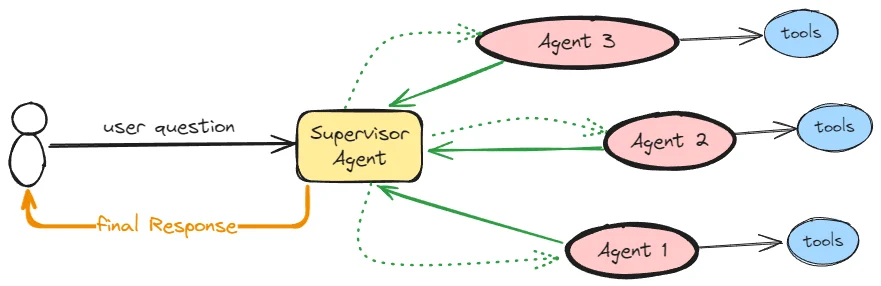
\includegraphics[width=0.9\linewidth]{Figures/agentic_workflow.png}
  \caption{A multi-agent system: a conversation between an orchestrator and specialists.}
  \label{fig:agents}
\end{figure}

\section{Governed agentic assistance for authoritative systems}
\label{sec:governed}

Integrating a probabilistic model into a deterministic analytical product raises
a central tension. A language model is fluent and helpful but may hallucinate,
misread intent, or be manipulated through content hidden in its inputs
\cite{greshake2023}. An analytical product, by contrast, derives its value from
reproducibility and auditability. An autonomous chatbot that silently mutated
assumptions or generated final figures would destroy exactly the property that
makes the tool trustworthy.

The appropriate design is therefore \textbf{bounded orchestration}: the assistant
may reason, retrieve, and propose, but it does not hold authority over state or
over numbers. Four principles enforce this separation. First, a \textbf{read /
write split}: read operations execute immediately, while any state-changing
action becomes a proposal. Second, \textbf{typed proposals}: model output is
converted into a structured, schema-checked payload rather than free text. Third,
\textbf{human-in-the-loop approval}: a user explicitly accepts a proposal before
it mutates the project or launches computation. Fourth, \textbf{deterministic
final authority}: even a successful assisted step only prepares inputs, while the
operational and financial results still come from the optimization engine. To
these, grounding techniques such as retrieval-augmented generation
\cite{lewis2020rag} add the requirement that generated statements be anchored to
retrieved facts rather than to the model's parametric memory. Together, these
principles let assistance improve usability without becoming a source of
numerical truth.

\section{Result interpretation and visualization for analytical software}
\label{sec:interp-foundations}

An analytical tool creates value only when its outputs support a decision. The
study of the existing platform showed that its results were available but not
interpreted: the burden of turning a population of simulations into an
operational and financial story fell entirely on the user. Two complementary
capabilities address this gap.

The first is \textbf{visualization}. Interactive exploration, such as scatter
plots with selectable axes and drill-down financial tables, lets a user compare
scenarios and locate the drivers of value before examining a single run in
detail. Effective visualization is not decoration; it is the interface through
which a large result set becomes legible.

The second is \textbf{grounded natural-language interpretation}. Building on the
tool-augmented reasoning described above, a language model can narrate what a
result means, which configuration produced it, and where its value comes from,
provided every figure it cites is read from the deterministic output rather than
computed by the model. The design challenge is precisely this grounding: the
explanation must be fluent and useful while remaining fully traceable to
simulation facts, with no invented numbers. This combination of interactive
visualization and grounded interpretation is at the heart of the work
detailed in Chapters~4 and~5.

\section{Evaluating and observing LLM-based systems}
\label{sec:eval-foundations}

A capability that relies on a language model cannot be validated by unit tests
alone: the same intent can be phrased in countless ways, and correctness is often
a matter of behavior (grounded, sound, appropriately cautious) rather than an
exact string. Evaluating such systems therefore requires dedicated methods.

For free-text outputs such as interpretations, the \textbf{LLM-as-a-judge}
approach uses an independent model, guided by an explicit rubric, to score
responses along dimensions such as faithfulness to the retrieved data and
soundness of the reasoning \cite{zheng2023judge}. Because a single judgement is
noisy, scores are aggregated over repeated evaluations and tracked across
versions. For structured outputs such as a generated topology, comparison against
a reference is better captured by a structural metric: the \textbf{graph edit
distance} measures the minimum number of edits needed to turn one graph into
another \cite{sanfeliu1983}, giving a fidelity score that plain string matching
cannot. These offline methods are complemented by \textbf{observability}: tracing
every model call, tool invocation, cost, and evaluator score, so that behavior
can be inspected, debugged, and compared in production, for which open platforms
such as Langfuse are designed \cite{langfuse2025}. Together these methods form
the methodology behind the evaluation harness developed in this work
(Figure~\ref{fig:eval-methods}).

\begin{figure}[H]
  \centering
  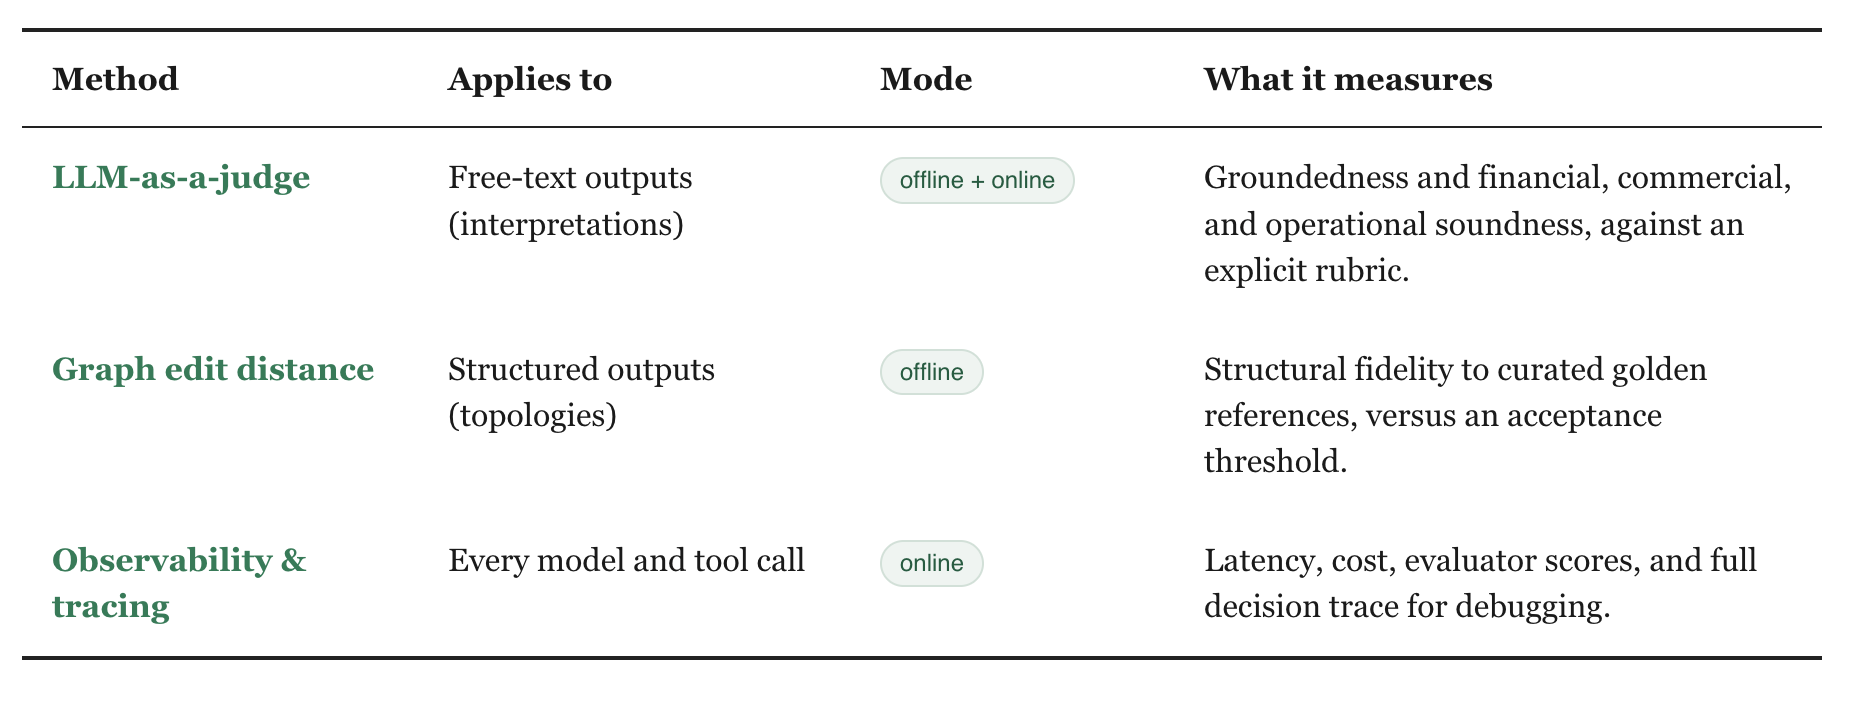
\includegraphics[width=\linewidth]{Figures/evaluation_methods.png}
  \caption{Complementary methods for evaluating the assisted capabilities.}
  \label{fig:eval-methods}
\end{figure}

\section{Enterprise foundations}
\label{sec:enterprise-foundations}

Two further axes frame the platform work carried out by the team. On identity,
enterprise analytical tools are expected to delegate authentication to a
federated identity provider through standard protocols such as OpenID Connect,
rather than operating a self-hosted identity stack, which reduces the security
surface owned by the application. On delivery, modern products rely on
infrastructure-as-code, automated builds and tests, container images, and
operational monitoring to remain deployable and reproducible. For an internal
product adapted across several clients, these are product requirements rather
than one-off engagement concerns: they determine whether the same core can be
delivered reliably to each new adaptation.

\section{Benchmarking and technical justification}
\label{sec:benchmark}

The direction can be justified by comparing candidate approaches against the
requirements observed in the existing platform. No isolated approach satisfies
the analytical, usability, trust, and operational requirements at the same time.
Table~\ref{tab:benchmark} summarizes the comparison.

\begin{table}[H]
  \centering
  \small
  \begin{tabularx}{\linewidth}{@{}>{\raggedright\arraybackslash}p{3.2cm} >{\raggedright\arraybackslash}X >{\raggedright\arraybackslash}X@{}}
    \toprule
    \textbf{Approach} & \textbf{Main limitation} & \textbf{Implication for the ETO} \\
    \midrule
    Manual / spreadsheet analysis & Flexible but weak in traceability, scalability,
      and reproducibility. & Useful for early reasoning, unsuitable as the
      computational authority. \\
    \addlinespace
    Solver-backed optimization & Strong numerical authority but insufficient alone
      for guidance, security, and usability. & Preserve the deterministic engine;
      improve the surrounding product. \\
    \addlinespace
    Cloud-native platform practices & Improve delivery reliability but do not solve
      modeling or interpretation. & Use as an engineering foundation for
      maintainable evolution. \\
    \addlinespace
    Self-hosted identity & Provides control but increases the security surface and
      operational burden. & Replace with federated enterprise OIDC. \\
    \addlinespace
    Workflow-oriented UX & Improves adoption but must stay connected to model
      constraints and validation. & Redesign the interface around guided workflows. \\
    \addlinespace
    Autonomous LLM chatbot & Improves interaction but can hallucinate or silently
      mutate state. & Reject autonomy; adopt bounded, approval-gated assistance. \\
    \addlinespace
    \textbf{Governed agentic assistance} & Requires careful design of tools,
      validation, and evaluation. & \textbf{The chosen direction}: assist without
      holding numerical authority. \\
    \bottomrule
  \end{tabularx}
  \caption{Comparison of candidate approaches.}
  \label{tab:benchmark}
\end{table}

The comparison shows that the appropriate response is not a single technology but
a combination that matches each requirement to the right solution family. That
combination is the target direction set out next.

\section{Target direction: governed modernization}
\label{sec:target}

The chosen direction is a \textbf{governed modernization} of the existing
platform rather than a rewrite: it preserves what is sound and redesigns what
limits adoption, across five decisions.

\begin{itemize}
  \item \textbf{Preserve the deterministic core} as the sole source of numerical
    truth; assisted work prepares inputs and explanations, never final results.
  \item \textbf{Restore the engineering and deployment foundation}, with
    reproducible delivery, infrastructure-as-code, and operational observability.
  \item \textbf{Migrate to federated enterprise identity} (OIDC), removing the
    self-hosted identity surface from the application stack.
  \item \textbf{Redesign the experience around guided workflows}, making the
    model easier to use without hiding its constraints or its validation.
  \item \textbf{Introduce governed agentic assistance}: typed proposals, system
    validation, and explicit human approval before any state change, with the
    optimizer retaining numerical authority.
\end{itemize}

\section{Positioning of the work}
\label{sec:positioning}

Within this direction, the work presented in this report concentrates on
the axes where the existing platform was weakest and where language models offer
the most leverage. The gap is not the solver but the product around it, and in
particular two of its facets: results that were produced but not interpreted, and
an assistant capability that, to be trustworthy, must be measured rather than
assumed.

Accordingly, the three pillars developed in the following chapters are the
\textbf{result-interpretation agent} (a grounded, read-only explainer of
simulation economics), the \textbf{visualization layer} that surfaces and
supports that interpretation, and the \textbf{evaluation harness} that measures
the grounding and soundness of the explanations produced. Each rests directly on
the foundations laid in this chapter: techno-economic indicators to be explained,
tool-augmented and governed language-model reasoning, and dedicated evaluation and
observability methods.

\section*{Conclusion}

This chapter studied the existing Energy Transition Optimizer, established the
technical foundations of the project axis by axis, and justified the choice of a
governed modernization that preserves the deterministic core while making it
accessible and trustworthy. It also positioned the work around result
interpretation, visualization, and evaluation. The next chapter turns this
positioning into an explicit specification of the functional and non-functional
requirements.


\chapter{Requirements Analysis and Specification}
\label{chap:requirements}

\section*{Introduction}

This chapter turns the direction chosen in Chapter~\ref{chap:background} into an
explicit specification. It identifies the actors that interact with the governed
assistant, states the functional requirements grouped by capability, then the
non-functional requirements that give the system its trustworthiness, lists the
constraints under which the work was carried out, and finally prioritizes the
requirements.

The requirements were derived from three sources: the analysis of the existing
platform (Chapter~\ref{chap:background}), the problem statement and objectives
set out in Chapter~\ref{chap:context}, and iterative discussion with the product
team during the internship.

\section{Actors and stakeholders}
\label{sec:actors}

The governed assistant is used by, and must satisfy, several categories of
actor. They differ in expertise and in the authority they hold over the system.

\begin{description}
  \item[Non-technical analyst.] The primary target user. Able to reason about a
    Power-to-X project in business terms, but not necessarily able to hand-build
    a topology or configure a grid search. Interacts mainly through natural
    language and expects to design, run, and above all \emph{understand} a study
    without mastering the model's internals.
  \item[Expert user.] A specialist who already knows the engine. Uses the
    assistant to move faster (drafting a topology, filling parameters, explaining
    a run) but retains the ability to work directly with the deterministic
    product and to judge the assistant's proposals.
  \item[Reviewer / approver.] The human in the loop. Any actor who inspects a
    proposed state change (a topology edit, an assumption update, a grid-search
    submission) and explicitly approves or rejects it before it takes effect.
    In practice the analyst and the expert both play this role.
  \item[BCG~X product team.] The owners and builders of the product, including
    the author of this report. Responsible for correctness, maintainability,
    evaluation, and safe evolution across client adaptations.
  \item[Operations and quality.] The role that observes the deployed system:
    traces, costs, evaluator scores, and platform health. Consumes the
    observability and monitoring outputs rather than the analytical results.
\end{description}

Figure~\ref{fig:usecase} gives a visual overview of the actors and the use cases
they exercise, and Table~\ref{tab:actors} lists the same mapping in detail.

\begin{figure}[H]
  \centering
  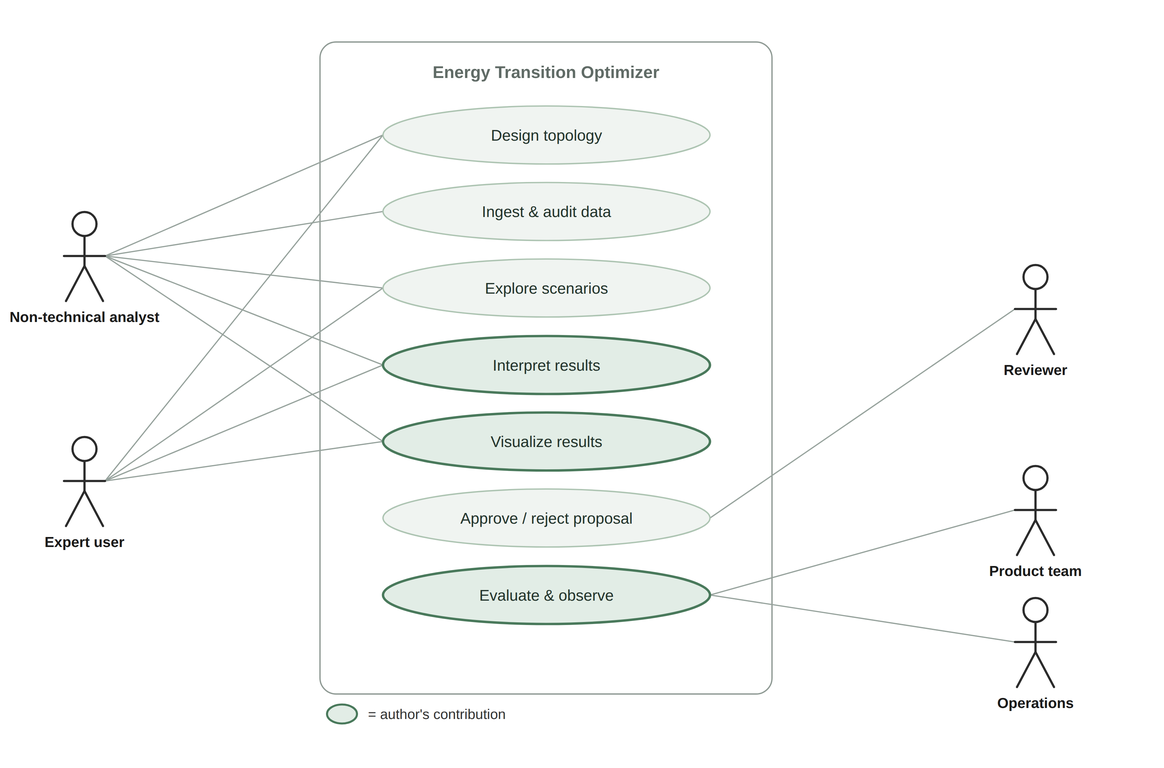
\includegraphics[width=\linewidth]{Figures/usecase.png}
  \caption{Use-case diagram of the governed assistant.}
  \label{fig:usecase}
\end{figure}

\begin{table}[H]
  \centering
  \small
  \begin{tabularx}{\linewidth}{@{}>{\raggedright\arraybackslash}p{3.2cm} >{\raggedright\arraybackslash}X@{}}
    \toprule
    \textbf{Actor} & \textbf{Main use cases} \\
    \midrule
    \textbf{Non-technical analyst} & Design a topology; ingest and audit data;
      explore scenarios; interpret results; visualize results;
      approve or reject proposals. \\
    \addlinespace
    \textbf{Expert user} & All of the above, plus direct use of the deterministic
      product and judgement of proposals. \\
    \addlinespace
    \textbf{Reviewer / approver} & Approve or reject a proposed state change before
      it takes effect. \\
    \addlinespace
    \textbf{BCG~X product team} & Build and maintain the capabilities;
      evaluate assistant behavior; adapt the product for each client. \\
    \addlinespace
    \textbf{Operations and quality} & Observe traces, costs, evaluator scores, and
      platform health. \\
    \bottomrule
  \end{tabularx}
  \caption{Actors and their main use cases.}
  \label{tab:actors}
\end{table}

\section{Functional requirements}
\label{sec:functional}

The functional surface is grouped into capabilities, each stated as a
requirement. These capabilities map onto the stages of a pre-feasibility
study (Figure~\ref{fig:study-workflow}).

\begin{figure}[H]
  \centering
  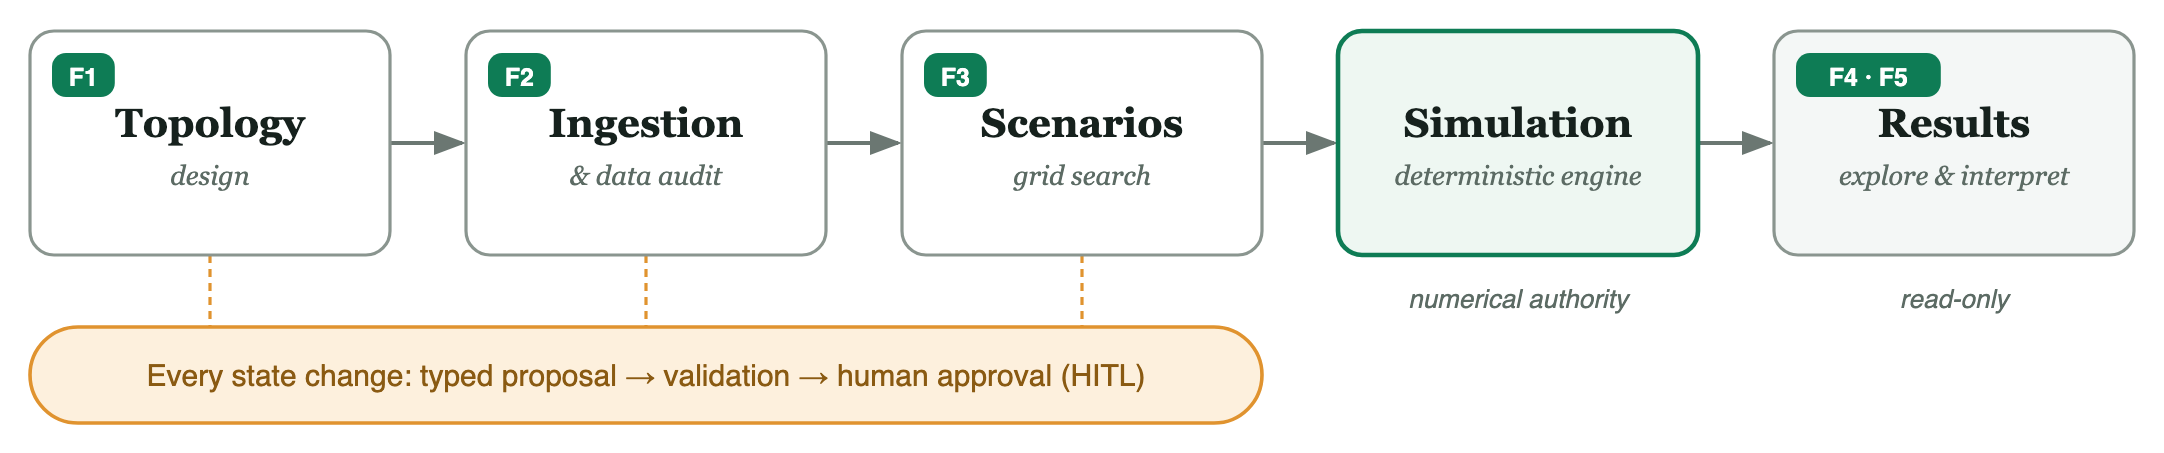
\includegraphics[width=\linewidth]{Figures/study_workflow.png}
  \caption{The end-to-end pre-feasibility study workflow the requirements target,
    with the approval gate on every state-changing stage.}
  \label{fig:study-workflow}
\end{figure}

\begin{description}
  \item[F1. Guided topology design.] From a natural-language description, the
    assistant shall propose a valid project topology (assets, buses, markets, and
    admissible flows), or edit an existing one, and surface the result as a
    reviewable proposal rather than a direct mutation.
  \item[F2. Assumption ingestion and audit.] The assistant shall load uploaded
    assumption files, classify and place their records, detect conflicts with
    existing project data, and return an approval-gated data-quality report.
  \item[F3. Scenario exploration.] The assistant shall help a user turn an intent
    into a bounded set of scenarios (a grid search), proposing sweep values
    across the technical, commercial, financial, and external dimensions, and
    returning a single validated set of operations for approval.
  \item[F4. Result interpretation.] Given a completed simulation
    population, the assistant shall explain, in natural language, which run is
    best, what drives its economics, and which parameters are worth examining,
    with every figure it states traceable to a deterministic result.
  \item[F5. Results visualization.] The interface shall let a user
    explore outputs interactively, including scatter plots with selectable axes
    and a navigable discounted-cash-flow table, and shall offer an
    interpret-on-demand action that attaches a grounded explanation to a chart.
  \item[F6. Governed state changes.] Every state-changing action (topology edit,
    assumption update, scenario submission) shall be expressed as a typed
    proposal, validated against schema and domain rules, and applied only after
    explicit human approval.
  \item[F7. Evaluation of assisted behavior.] The system shall provide
    a means to measure the quality of assistant outputs, scoring the grounding
    and soundness of interpretations and the fidelity of generated structures,
    in a repeatable way across versions.
  \item[F8. Observability and monitoring.] The system shall record traces, model
    usage, and evaluator scores for assisted interactions, and shall support
    periodic health assessment of the deployed platform.
\end{description}

\subsection{Detailed use case: interpreting a completed grid search}

Because result interpretation is central to this work, it is specified as a
detailed scenario.

\begin{description}
  \item[Actor.] Non-technical analyst.
  \item[Precondition.] A grid search has completed and its results are persisted;
    the analyst is viewing the results of a project.
  \item[Main flow.] (1)~The analyst asks, in plain language, to explain a run or
    a chart. (2)~The assistant retrieves the relevant simulation metrics,
    financial breakdowns, and chart context through read-only tools. (3)~It
    produces a streamed narration and a set of insight cards, citing only figures
    read from the deterministic output. (4)~It may embed the relevant chart next
    to the explanation.
  \item[Postcondition.] The analyst obtains a grounded interpretation. No project
    state is modified (the interpreter is read-only), so no approval is required.
  \item[Alternative flow.] If the evidence is insufficient to support a claim
    (for example inferring a correlation from a single point), the assistant
    states the limitation instead of overreaching.
\end{description}

Figure~\ref{fig:interp-usecase} illustrates this scenario on a real study.

\begin{figure}[H]
  \centering
  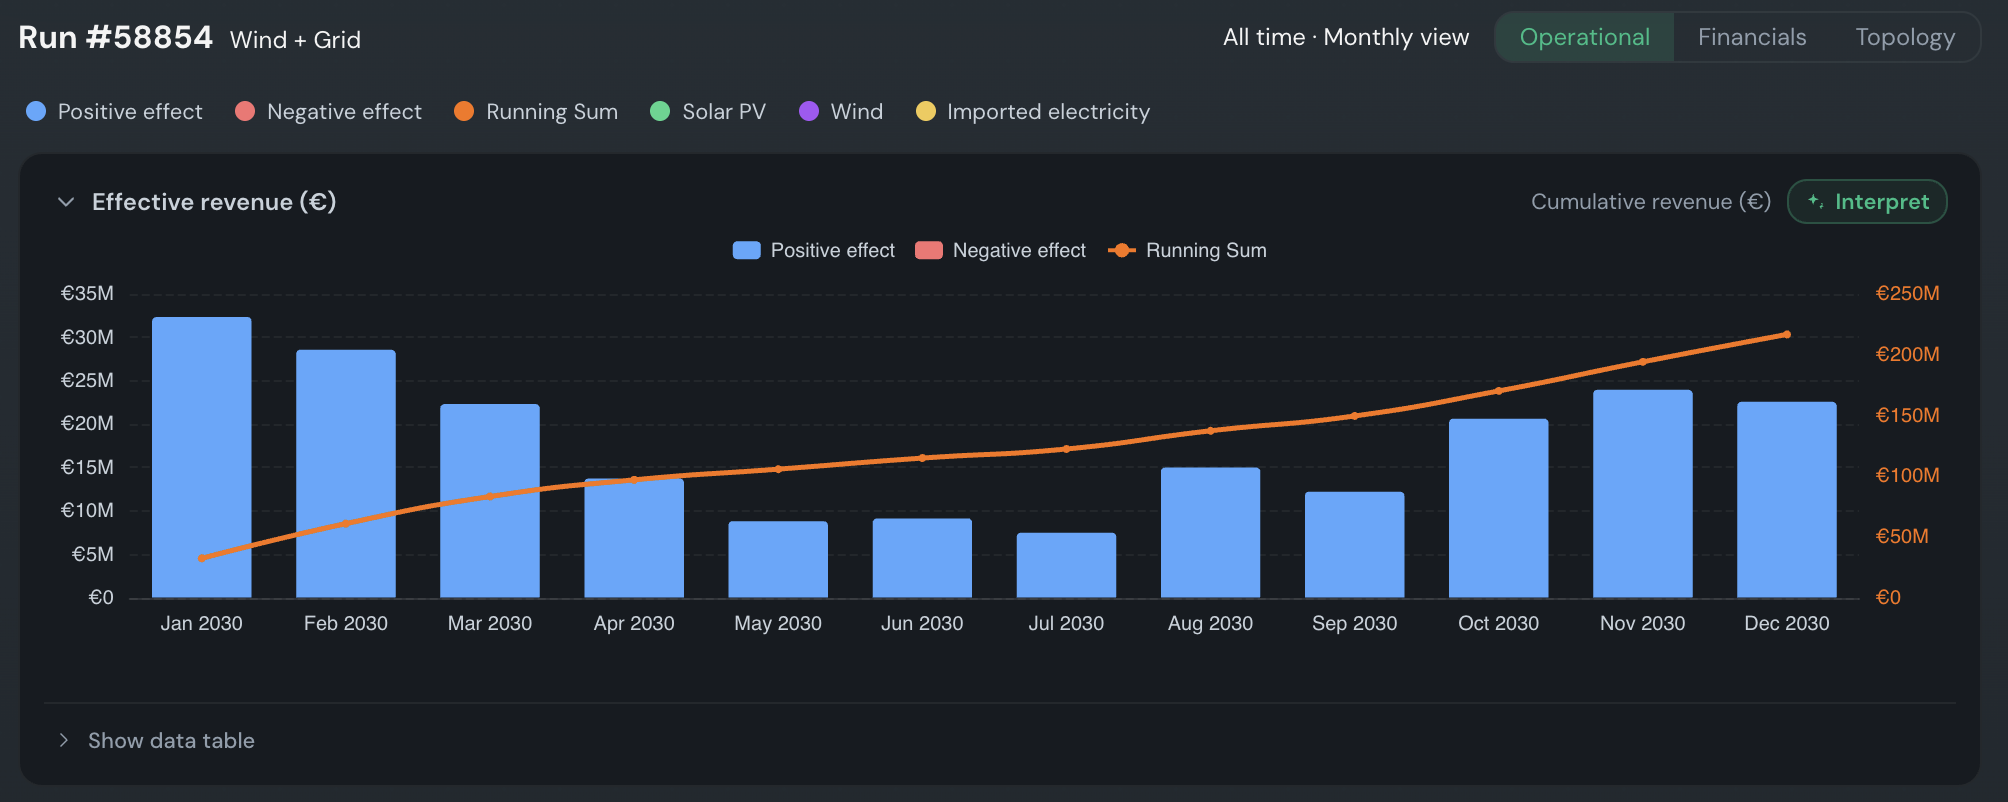
\includegraphics[width=\linewidth]{Figures/1.png}\\[0.3cm]
  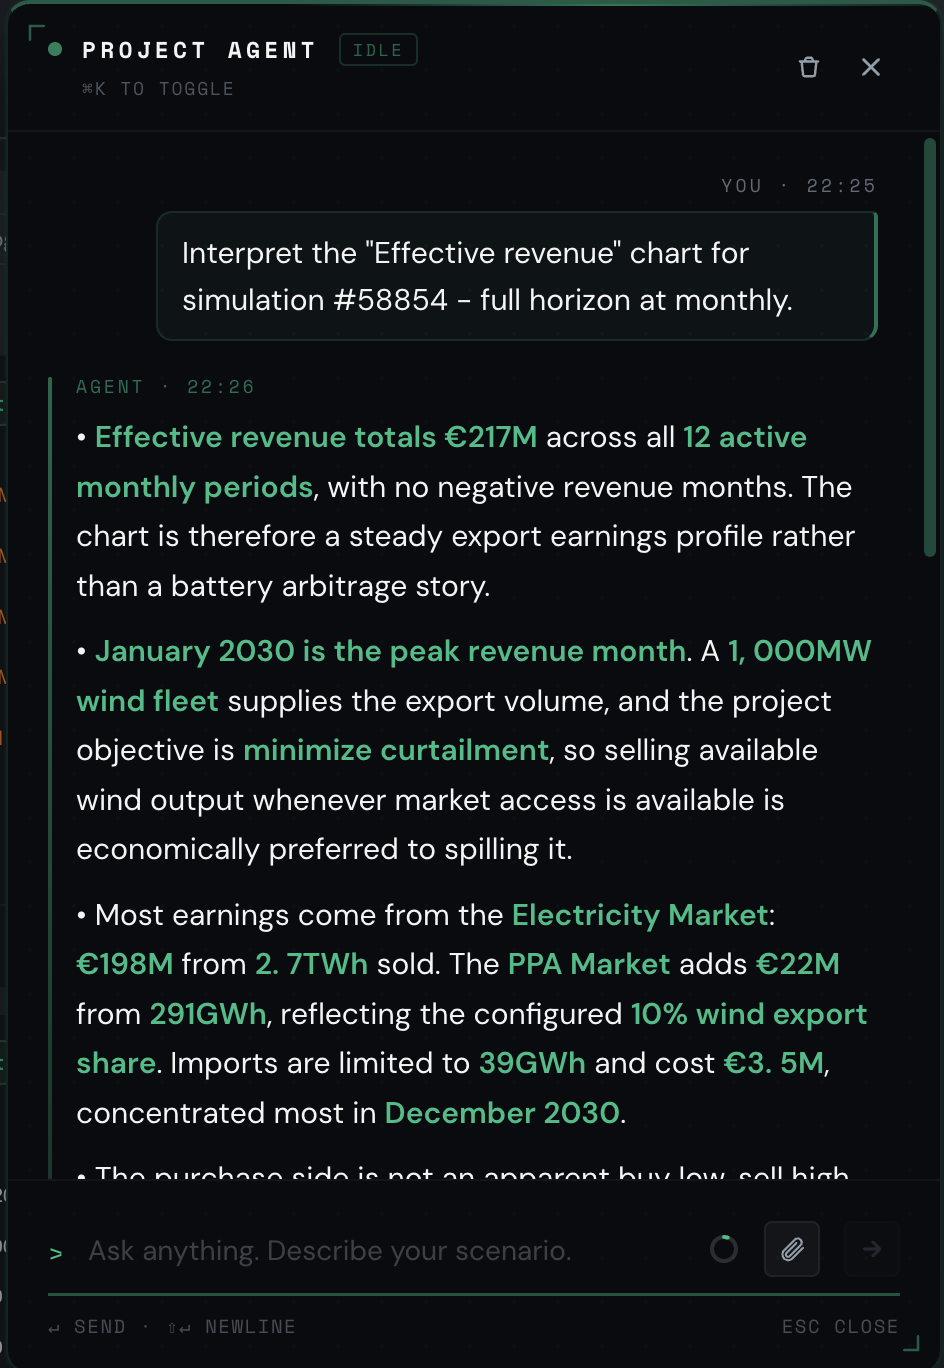
\includegraphics[width=0.32\linewidth]{Figures/2-1.png}
  \hfill
  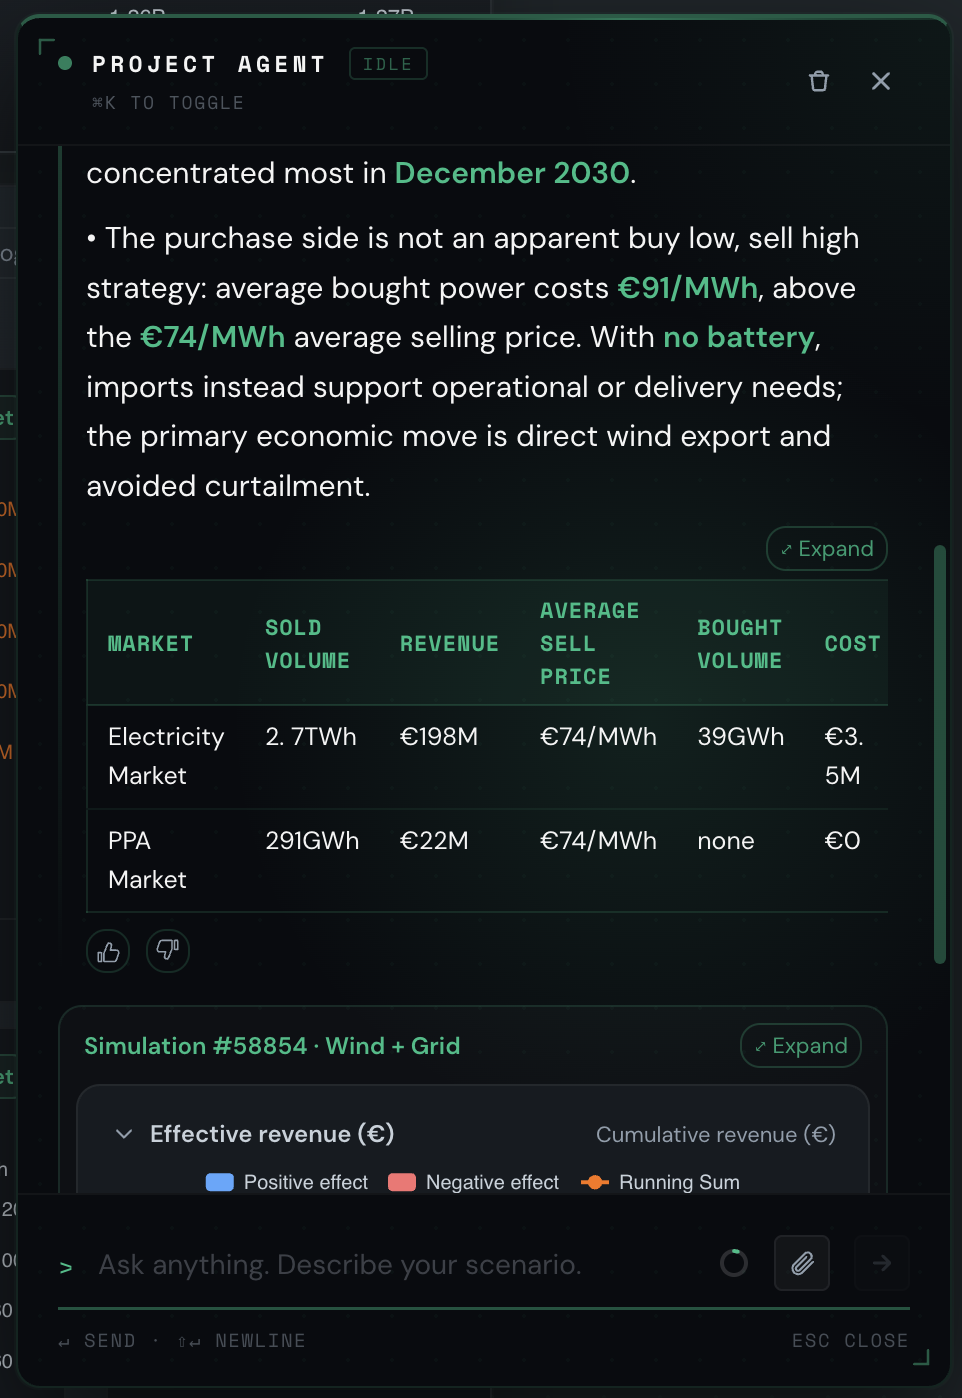
\includegraphics[width=0.32\linewidth]{Figures/2-2.png}
  \hfill
  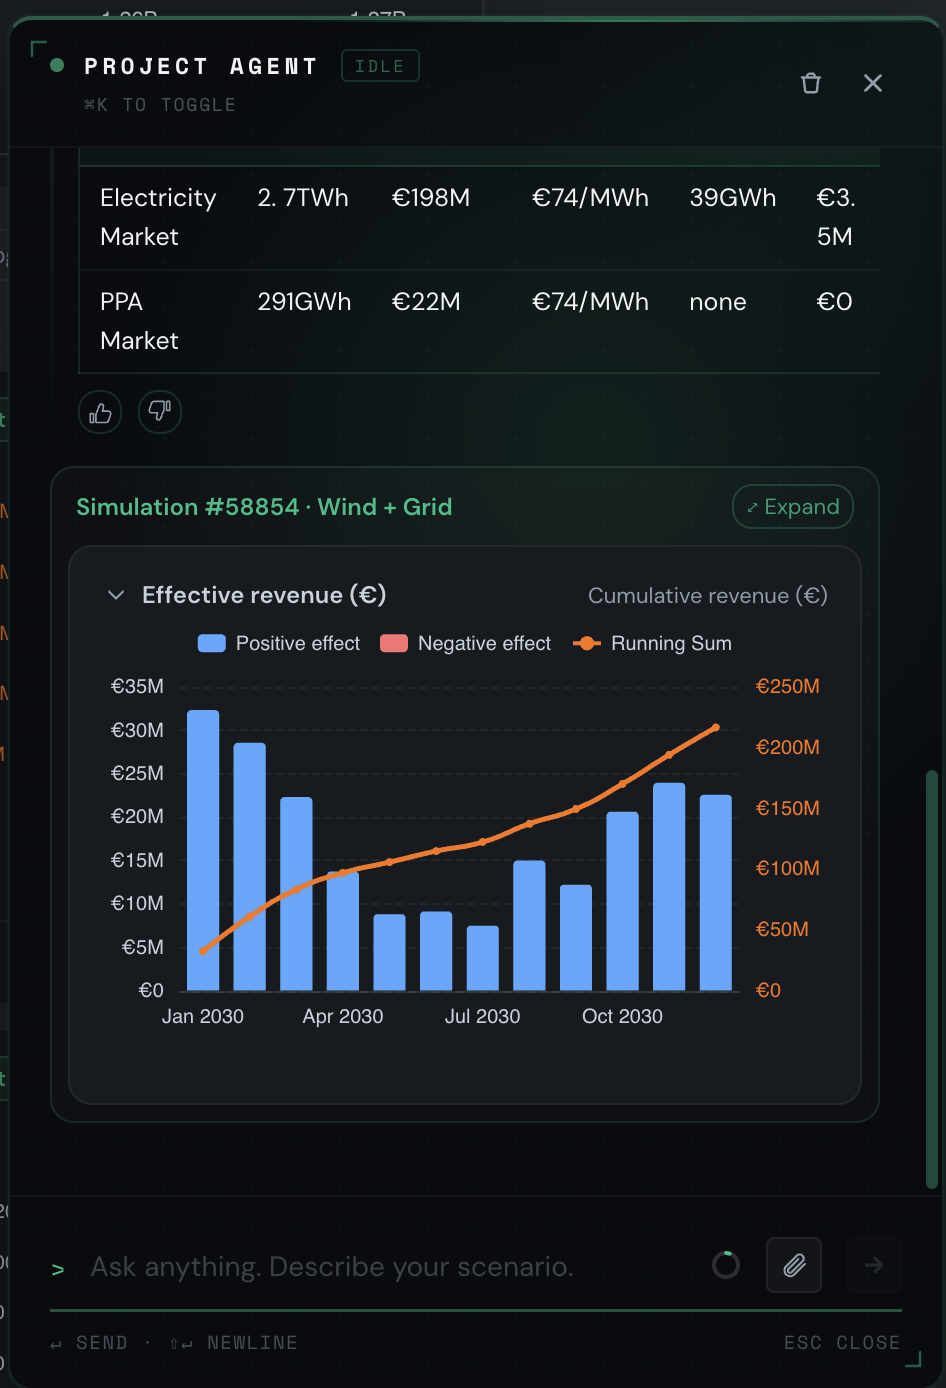
\includegraphics[width=0.32\linewidth]{Figures/2-3.png}
  \caption{The interpreter agent use case.}
  \label{fig:interp-usecase}
\end{figure}

\subsection{Detailed use case: editing a topology under approval}

This second scenario illustrates the governed \emph{write} path, where an action
does change project state and therefore passes through the approval gate.

\begin{description}
  \item[Actor.] Non-technical analyst (with a reviewer, often the same person).
  \item[Precondition.] A project exists; the analyst wants to add or modify an
    asset (for example, ``add a battery and a second electrolyzer'').
  \item[Main flow.] (1)~The analyst describes the change in plain language.
    (2)~The assistant gathers context and generates a candidate topology, then
    validates it against schema and domain rules. (3)~It surfaces the change as a
    \textbf{typed proposal} (a review card), not a direct mutation. (4)~The
    reviewer inspects the proposal and \textbf{approves} it. (5)~Only then is the
    project topology updated. Figure~\ref{fig:topology-design-approval} shows the
    proposal and its approval card.

\begin{figure}[H]
  \centering
  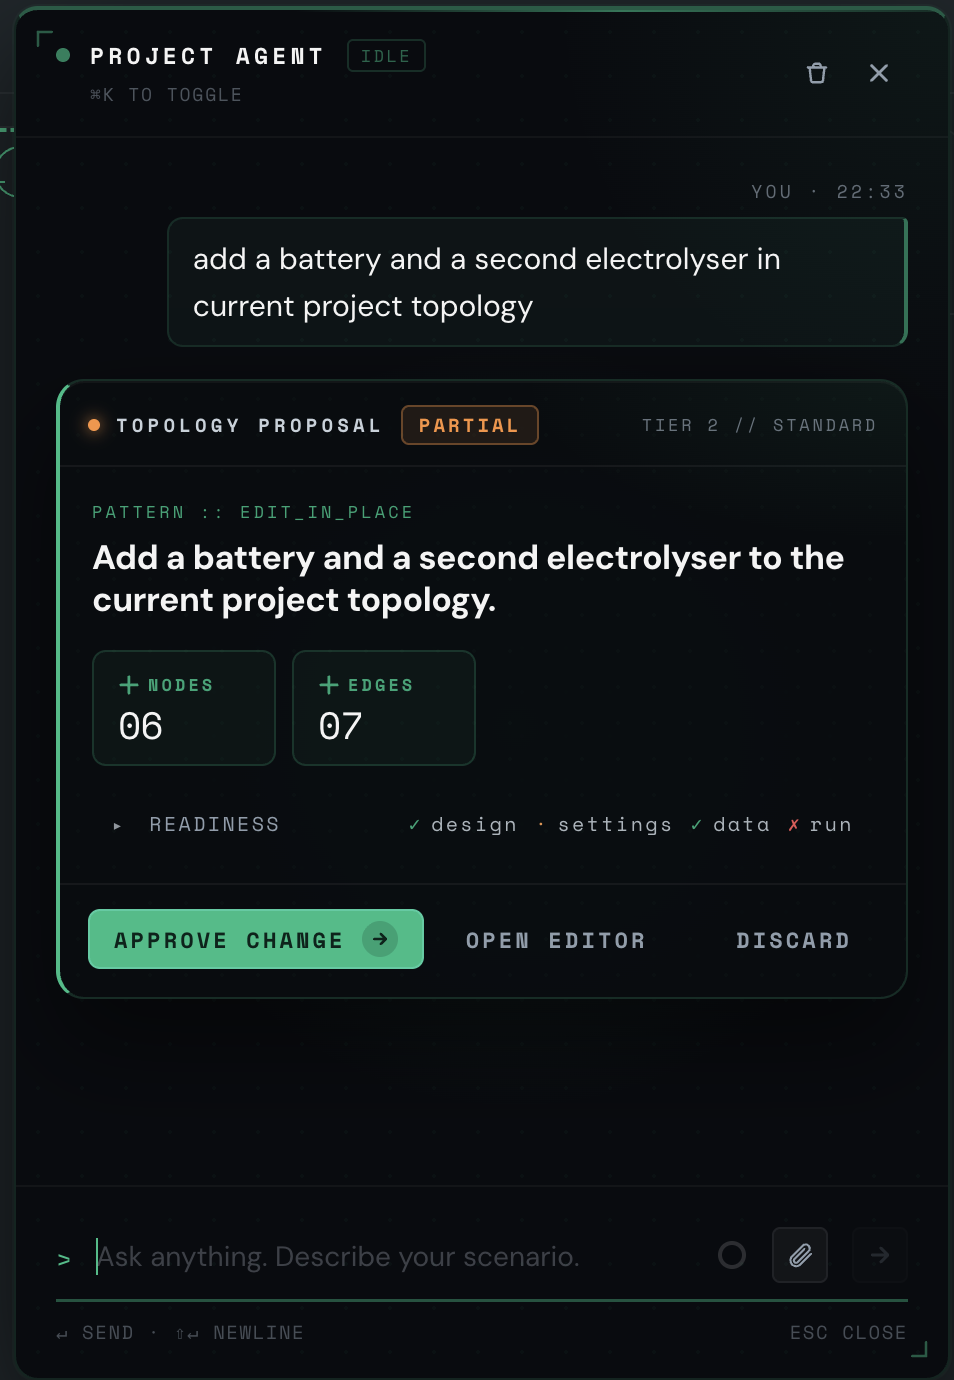
\includegraphics[width=0.48\linewidth]{Figures/a1.png}
  \hfill
  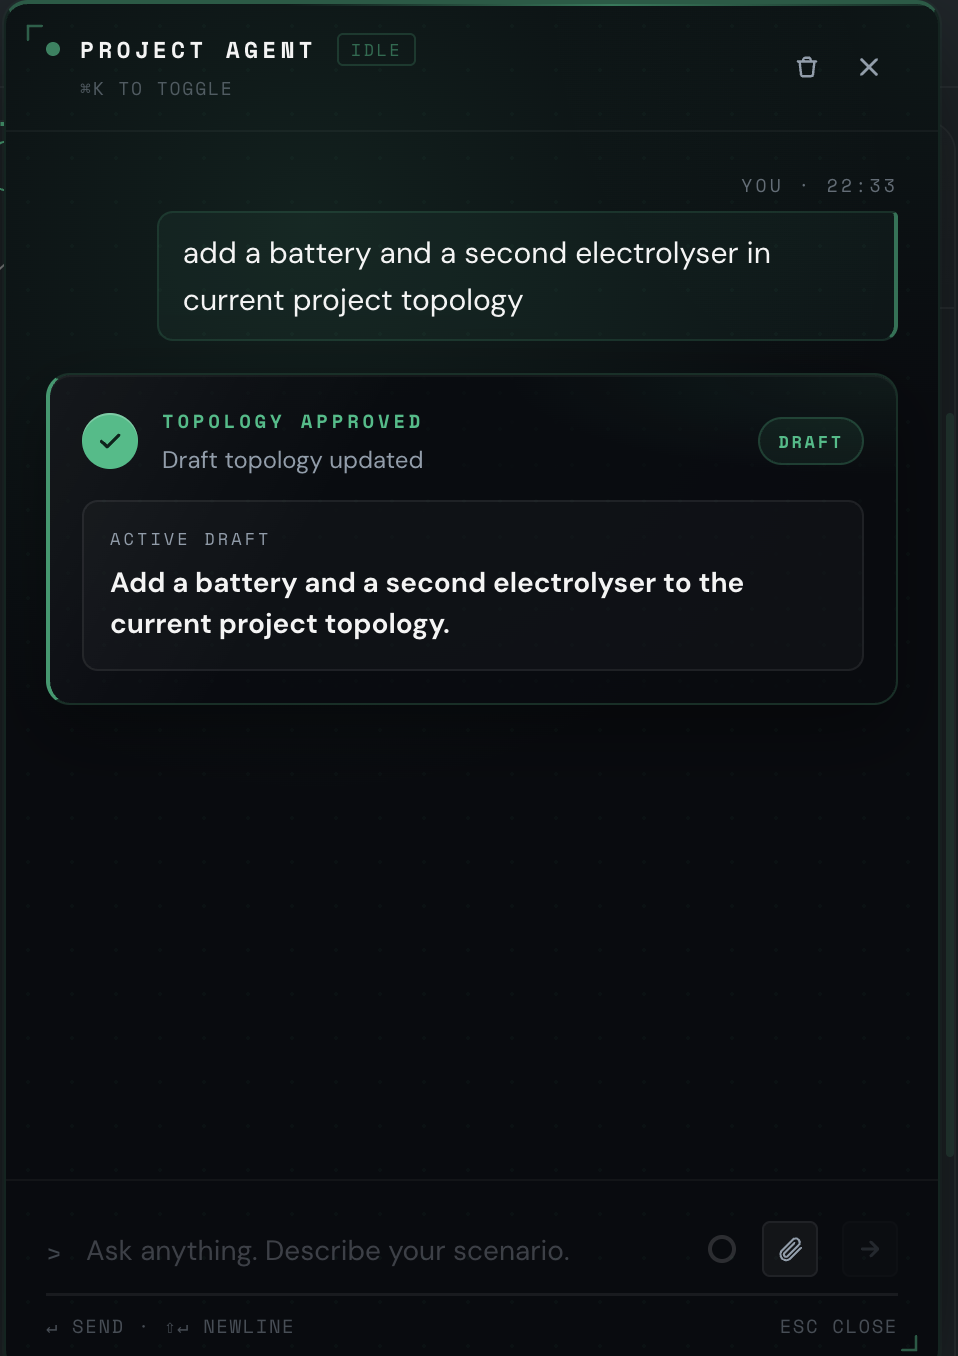
\includegraphics[width=0.48\linewidth]{Figures/a2.png}
  \caption{The topology design use case.}
  \label{fig:topology-design-approval}
\end{figure}

  \item[Postcondition.] The topology is modified in a traceable way, or left
    unchanged if the proposal is rejected.
  \item[Alternative flow.] If validation fails, the assistant blocks the proposal
    and returns the failing evidence rather than applying a broken design; the
    analyst can refine the request and retry.
\end{description}

\section{Non-functional requirements}
\label{sec:nonfunctional}

The non-functional requirements are what make the assistant trustworthy enough to
be used on real analyses; they matter as much as the functional surface.
Table~\ref{tab:nfr} states them with their rationale, and they fall into a few
families. Two express the central principle that the optimizer, not the model, is
the source of truth: \emph{numerical authority} (NF1) and \emph{groundedness}
(NF2), the latter being the property the evaluation harness later measures
directly. Two concern trust in operation, \emph{reproducibility and auditability}
(NF3) and \emph{human control} (NF4), which together make every assisted action
repeatable and reversible under explicit approval. \emph{Responsiveness} (NF5)
keeps the interface usable despite model and simulation latency, and
\emph{evaluability and observability} (NF6) makes agent behavior measurable and
inspectable rather than assumed. Finally, \emph{security and enterprise identity}
(NF7) and \emph{maintainability and adaptability} (NF8) are product-level qualities
that let the same core be operated safely and adapted for each client.

Where useful these carry concrete, testable targets. Interpretations begin
streaming within a short first-token budget rather than blocking on the full
answer (NF5). Structured outputs such as generated topologies are accepted only
above a fixed graph-edit-similarity threshold, set at $0.85$ and tracked across
versions (NF6, Chapter~\ref{chap:implementation}). Interpretations are scored by an
independent judge on groundedness and on financial, commercial, and operational
soundness (NF2, NF6). And every assisted interaction is traced end to end together
with its model usage and evaluator scores (NF6).

\begin{table}[H]
  \centering
  \small
  \begin{tabularx}{\linewidth}{@{}>{\bfseries}l >{\raggedright\arraybackslash}p{3.4cm} >{\raggedright\arraybackslash}X@{}}
    \toprule
    \textbf{Ref.} & \textbf{Requirement} & \textbf{Why it matters} \\
    \midrule
    NF1 & Numerical authority & The deterministic engine remains the sole source
      of results; no figure shown to a user originates from the model. \\
    \hypertarget{nf:groundedness}{NF2} & Groundedness & Every quantitative statement
      is traceable to a specific deterministic output, with no invented numbers. \\
    NF3 & Reproducibility \& auditability & The same inputs give the same results,
      and assisted actions are inspectable after the fact. \\
    NF4 & Human control & No state change takes effect without explicit approval;
      destructive operations are reversible where possible. \\
    NF5 & Responsiveness & Interpretations stream token by token, and long
      computations never block the interface. \\
    \hypertarget{nf:eval}{NF6} & Evaluability \& observability & Behavior is
      measurable through a repeatable harness and observable through end-to-end
      tracing. \\
    NF7 & Security \& enterprise identity & Access is mediated by the enterprise
      identity provider; the application runs no identity stack of its own. \\
    NF8 & Maintainability \& adaptability & Reproducible deployment across the
      several modes, and adaptability to each client. \\
    \bottomrule
  \end{tabularx}
  \caption{Non-functional requirements and their rationale.}
  \label{tab:nfr}
\end{table}

\section{Constraints}
\label{sec:constraints}

Constraints differ from the non-functional requirements above: they are external
givens imposed on the work rather than quality targets it sets for itself. Several
are \emph{realized} by a non-functional requirement, noted below so the two are not
read as duplicates.

\begin{itemize}
  \item \textbf{Deterministic authority.} The founding premise of the project: the
    assistant assists and proposes but never computes final results. It is imposed
    here, and the design turns it into numerical authority (NF1) and human control
    (NF4).
  \item \textbf{Client confidentiality.} No client-identifying data appears in the
    product artifacts or in this report; the product is an internal asset adapted
    per client (Section~\ref{sec:internal-product}). This is a business and legal
    given, with no functional substitute.
  \item \textbf{Enterprise identity.} The host organization mandates that
    authentication be delegated to its own identity provider through OpenID
    Connect; the design meets this through NF7.
  \item \textbf{Model cost and latency.} Language-model calls carry a cost and a
    latency budget the work does not control; the design respects it (for example
    by reusing prior results and streaming output), the user-facing side of which
    is NF5.
\end{itemize}

Reproducibility across the local, container, and cloud modes is likewise required,
but as a quality target it is stated as a non-functional requirement (NF8) rather
than repeated here.

\section{Prioritization}
\label{sec:prioritization}

The functional requirements were prioritized using a MoSCoW scheme. Within the
scope of this report every functional requirement is either a \emph{Must} or a
\emph{Should}; none were deferred to \emph{Could} or \emph{Won't}, so those tiers
do not appear. The priorities reflect this phase of the work rather than a
from-scratch build order. Governed state changes
(F6) is \emph{Must} because it is the safety foundation every other capability
depends on: it is the condition under
which any assisted capability may touch project state. Result interpretation
(F4), visualization (F5), and evaluation (F7) are \emph{Must} because they close
the loop the project set out to deliver: results that can be explored, explained,
and trusted. Guided topology design (F1), ingestion (F2), scenario exploration
(F3), and observability (F8) are logically prior to interpretation in a study but
were largely already in place when this phase of the work began, so they are
\emph{Should}. The non-functional
requirements are treated as qualities that must hold throughout rather than ranked
on the same scale. Table~\ref{tab:prio} summarizes the result.

\begin{table}[H]
  \centering
  \small
  \begin{tabularx}{\linewidth}{@{}>{\bfseries}l >{\raggedright\arraybackslash}X >{\centering\arraybackslash}p{2.4cm}@{}}
    \toprule
    \textbf{Ref.} & \textbf{Requirement} & \textbf{Priority} \\
    \midrule
    F6 & Governed state changes & Must \\
    F4 & Result interpretation & Must \\
    F5 & Results visualization & Must \\
    F7 & Evaluation of behavior & Must \\
    F1 & Guided topology design & Should \\
    F2 & Assumption ingestion and audit & Should \\
    F3 & Scenario exploration & Should \\
    F8 & Observability and monitoring & Should \\
    \bottomrule
  \end{tabularx}
  \caption{Prioritization of functional requirements.}
  \label{tab:prio}
\end{table}

\section*{Conclusion}

This chapter specified the actors, the functional requirements grouped by
capability, the non-functional requirements that establish trust, the binding
constraints, and the prioritization of the work, with result interpretation,
visualization, evaluation, and governed state changes identified as the
capabilities the project had to deliver end to end. The next chapter presents
the design and architecture that satisfy these requirements.


\chapter{Design and Architecture of the Solution}
\label{chap:design}

\section*{Introduction}

This chapter presents the design that satisfies the requirements of
Chapter~\ref{chap:requirements}. It describes the platform as a whole: its
architectural objectives, its logical decomposition, its runtime and deployment
model, its security and trust boundaries, its persistence, and its simulation
workflow. It then details the governed multi-agent layer, agent by agent, and the
observability and operational architecture around it. The result-interpretation
agent, the visualization layer, and the evaluation harness, the components at the
heart of the report's central question, are presented in this same flow and given
deeper treatment, always as parts of the complete system rather than in
isolation.

The design is guided by one central constraint: the deterministic optimizer
remains the authority for operational and financial results. Every other
subsystem exists to make that authority easier to access, safer to operate, and
more efficient to use. A structural theme follows from this constraint and recurs
throughout the chapter: the platform keeps interactive coordination on the request
path separate from \textbf{two durable, asynchronous execution planes} off it, one
for deterministic simulation and one for agent reasoning. Heavy or probabilistic
work therefore never blocks the interface, each plane is dispatched durably and
recovered on its own, and neither can seize numerical authority.

\section{Architectural objectives and system role}
\label{sec:arch-objectives}

The design starts from the limitations identified earlier and translates them into
architectural objectives. Table~\ref{tab:objectives} states each objective and its
architectural implication.

\begin{table}[H]
  \centering
  \begin{tabularx}{\linewidth}{@{}
      >{\raggedright\arraybackslash}p{4.3cm}
      >{\raggedright\arraybackslash}X @{}}
    \toprule
    \textbf{Objective} & \textbf{Architectural implication} \\
    \midrule
    Preserve numerical authority & Keep optimization in the deterministic core;
      route assisted work toward validated inputs and approved actions rather than
      model-generated results. \\
    \addlinespace
    Support long-running computation & Separate interactive traffic from
      simulation through asynchronous dispatch, persisted job state, and
      independently managed compute. \\
    \addlinespace
    Protect enterprise access & Move identity enforcement to the platform edge
      through federated authentication, avoiding application-owned identity
      complexity. \\
    \addlinespace
    Improve maintainability & Give each concern (interaction, coordination,
      computation, persistence, assistance, platform) a clear owner. \\
    \addlinespace
    Make deployments repeatable & Treat infrastructure, runtime configuration, and
      releases as versioned delivery artifacts. \\
    \addlinespace
    Govern language-model assistance & Typed tool contracts, observable
      interactions, validation, and human approval before any mutation. \\
    \bottomrule
  \end{tabularx}
  \caption{Architectural objectives and their implications.}
  \label{tab:objectives}
\end{table}

The architecture is therefore not a single tooling choice but a set of
\textbf{boundaries}: between users and protected services, between synchronous
requests and asynchronous computation, between authoritative computation and
probabilistic assistance, and between product logic and operating-environment
concerns.

\section{Logical decomposition}
\label{sec:logical}

At the highest level the system is organized as a progression from interaction to
computation (Figure~\ref{fig:logical-layers}). Users work through a
\textbf{presentation layer}; a
\textbf{coordination layer} validates requests and coordinates state transitions;
long-running optimization is delegated to dedicated \textbf{execution} capacity;
durable stores hold canonical state and large artifacts; the \textbf{agentic
layer} assists through bounded proposals; and the \textbf{platform layer} provides
the secure operating envelope.

\begin{figure}[H]
  \centering
  \resizebox{0.9\linewidth}{!}{%
  \begin{tikzpicture}[
    font=\small,
    box/.style={rectangle, rounded corners=3pt, draw=black!55, thick,
      align=center, inner sep=5pt, fill=white, minimum height=0.8cm, text width=3.2cm},
    core/.style={rectangle, rounded corners=4pt, draw=teal!70!black, line width=1pt,
      align=center, inner sep=5pt, fill=teal!8, minimum height=0.8cm, text width=3.2cm},
    arr/.style={-{Stealth[length=2.5mm]}, line width=0.9pt, black!65},
    darr/.style={-{Stealth[length=2.5mm]}, line width=0.9pt, black!55, dashed},
  ]
    \node[box, text width=1.4cm] (user) {User};
    \node[box, below=0.7cm of user] (pres) {Presentation layer};
    \node[box, below=0.9cm of pres] (coordn) {Coordination layer\\(typed contracts)};
    \node[box, right=2.4cm of coordn] (agent) {Agentic layer\\(bounded proposals)};
    \node[core, below left=0.9cm and -1.4cm of coordn] (exec) {Deterministic execution};
    \node[box, below right=0.9cm and -1.4cm of coordn] (pers) {Persistence\\(state and artifacts)};
    \draw[arr] (user) -- (pres);
    \draw[arr] (pres) -- node[left, font=\footnotesize, black!60]
      {authenticated requests} (coordn);
    \draw[arr] (coordn) -- (exec);
    \draw[arr] (coordn) -- (pers);
    \draw[arr] (exec) -- (pers);
    \draw[arr] (coordn.15) -- node[above, font=\footnotesize, black!60]
      {assisted turns} (agent.165);
    \draw[darr] (agent.195) -- node[below, font=\footnotesize, black!60]
      {typed proposals} (coordn.345);
    \begin{scope}[on background layer]
      \node[rectangle, rounded corners=5pt, draw=black!25, fill=black!4,
        inner sep=10pt, fit=(coordn)(agent)(exec)(pers),
        label={[font=\footnotesize\bfseries, black!50]below:Platform layer
          (secure operating envelope)}] {};
    \end{scope}
  \end{tikzpicture}%
  }
  \caption{Logical decomposition: authority flows from the coordination layer to
    the deterministic core, while the agentic layer may only propose.}
  \label{fig:logical-layers}
\end{figure}

The important point is the direction of authority. User-facing and agentic
components may prepare, explain, and request changes, but state transitions pass
through the coordination layer, and numerical outputs pass through the
deterministic engine. This avoids two weak designs: exposing the solver directly
(forcing users to understand its internals) and hiding the solver behind an
autonomous conversational layer (weakening reproducibility and auditability).

\subsection{System graph views}

A useful way to reason about the architecture is to view it as a set of directed
graphs, each with its own nodes and its own authority rule
(Table~\ref{tab:graphs}). This makes explicit which component may transform state
and which may only request or observe it.

\begin{table}[H]
  \centering
  \begin{tabularx}{\linewidth}{@{}
      >{\raggedright\arraybackslash}p{3.1cm}
      >{\raggedright\arraybackslash}X @{}}
    \toprule
    \textbf{Graph} & \textbf{Nodes and authority rule} \\
    \midrule
    Runtime execution & Presentation, access boundary, coordination, asynchronous
      execution, persistence, observability. Interactive requests, simulation
      jobs, and observability events follow different edges; long-running
      optimization never blocks the request path. \\
    \addlinespace
    Domain topology & Project canvas, asset and market nodes, flow edges, scenario
      parameters. The user edits an application-level graph; the coordination
      layer validates it before it becomes an optimization input. \\
    \addlinespace
    Simulation & Submitted scenario, persisted input, dispatched job, deterministic
      execution, output artifacts. Heavy payloads move by reference, while the
      dispatch path carries identifiers and execution intent. \\
    \addlinespace
    Assisted action & User intent, Director, specialist reasoning, typed proposal,
      validation, approval, committed mutation. Model output may propose, but only
      validated and approved proposals mutate project state. \\
    \bottomrule
  \end{tabularx}
  \caption{System graph views and their authority rules.}
  \label{tab:graphs}
\end{table}

\section{Runtime and deployment architecture}
\label{sec:runtime}

The runtime separates interactive work on the request path from the two
asynchronous execution planes introduced above (Figure~\ref{fig:two-planes}). A
normal request enters through the presentation layer, crosses the authenticated
edge, and reaches the coordination layer, which either reads or updates project
state, serves assisted interactions, or dispatches work to one of the two planes.
The first runs \textbf{deterministic simulation}, described here; the second runs
the \textbf{agent reasoning system}, described in
Section~\ref{sec:agent-runtime}. Because a grid search can
launch thousands of hour-by-hour simulations and run far longer than a web request
should block for, simulation work is placed on an \textbf{asynchronous execution
path}: the backend enqueues a job on a dedicated queue, a separate pool of workers
consumes it, runs the deterministic engine, and persists the outputs for later
retrieval, while the interface stays responsive and polls for status.

This split is essential because it lets execution capacity scale independently of
interactive capacity: heavy workloads are absorbed by adding workers, so the
interactive experience stays responsive under load rather than competing with
computation for capacity. Scaling follows the same
separation, with backlog depth as the signal that drives additional execution
capacity, while the coordination side is scaled more conservatively so that
capacity improvements never compromise the correctness of conversational
checkpoint state.

\begin{figure}[H]
  \centering
  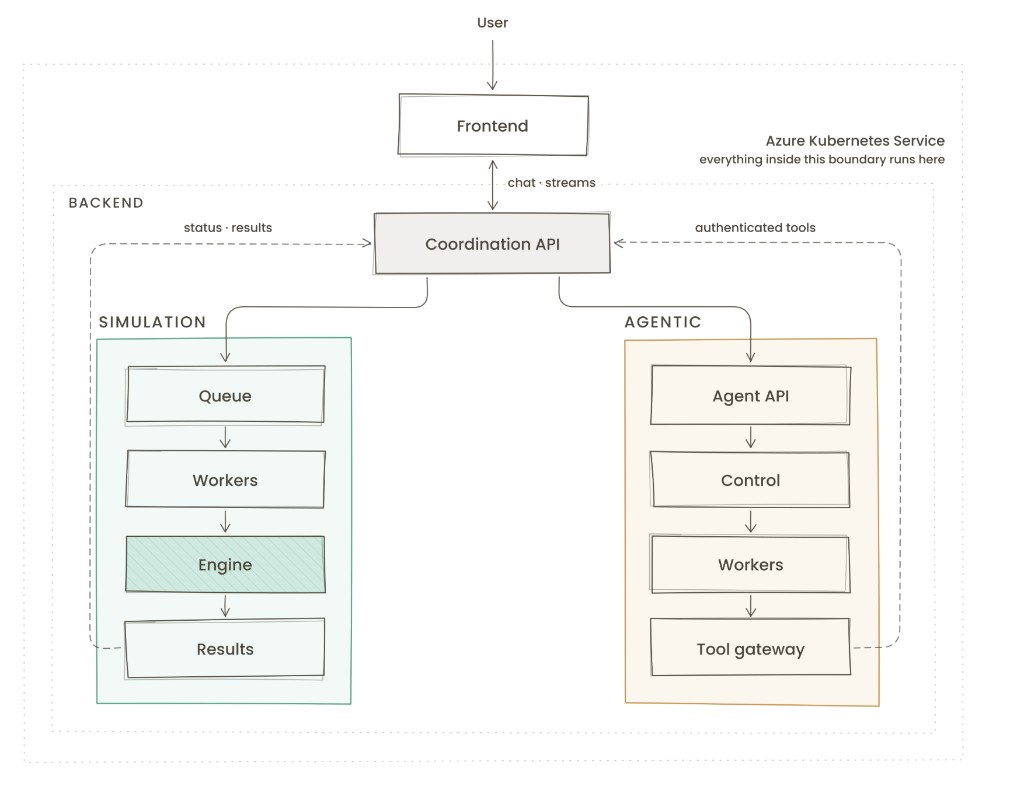
\includegraphics[width=0.9\linewidth]{Figures/runtime_planes.png}
  \caption{The application on Azure Kubernetes Service: the backend and the two
    durable execution planes, simulation and agentic, with their controlled
    return paths.}
  \label{fig:two-planes}
\end{figure}

\subsection{Cloud and deployment model}

The platform runs in a managed cloud environment rather than on manually operated
servers. The environment is separated into foundational resources (build, naming,
shared storage), infrastructure resources (private networking, controlled
administration, compute capacity, cost controls), and runtime support services
(access control, authentication support, observability, and operational
monitoring). Access to the environment is mediated through controlled paths rather
than direct public exposure, and source changes are built outside the private
environment and promoted inward through a controlled registry path.

Reflecting its nature as an internal product adapted across clients, the optimizer
ships in three modes that share the same core engine: a \textbf{standalone} mode
(a command-line interface running locally against a lightweight database, the
fastest way to get started), a \textbf{container-stack} mode (the full application
brought up together for end-to-end development), and a \textbf{cloud} mode (a
managed deployment that provides always-available interfaces, isolates resources,
and lets compute scale on demand). Infrastructure is described as code so that
each environment is reproducible and each client adaptation starts from the same
baseline. The application-level deployment on the cluster is shown in
Figure~\ref{fig:deployment-diagram}, and the underlying cloud infrastructure, its
private network, controlled administrative access, compute node pools, and managed
data services, in Figure~\ref{fig:azure-infra}.

\begin{figure}[H]
  \centering
  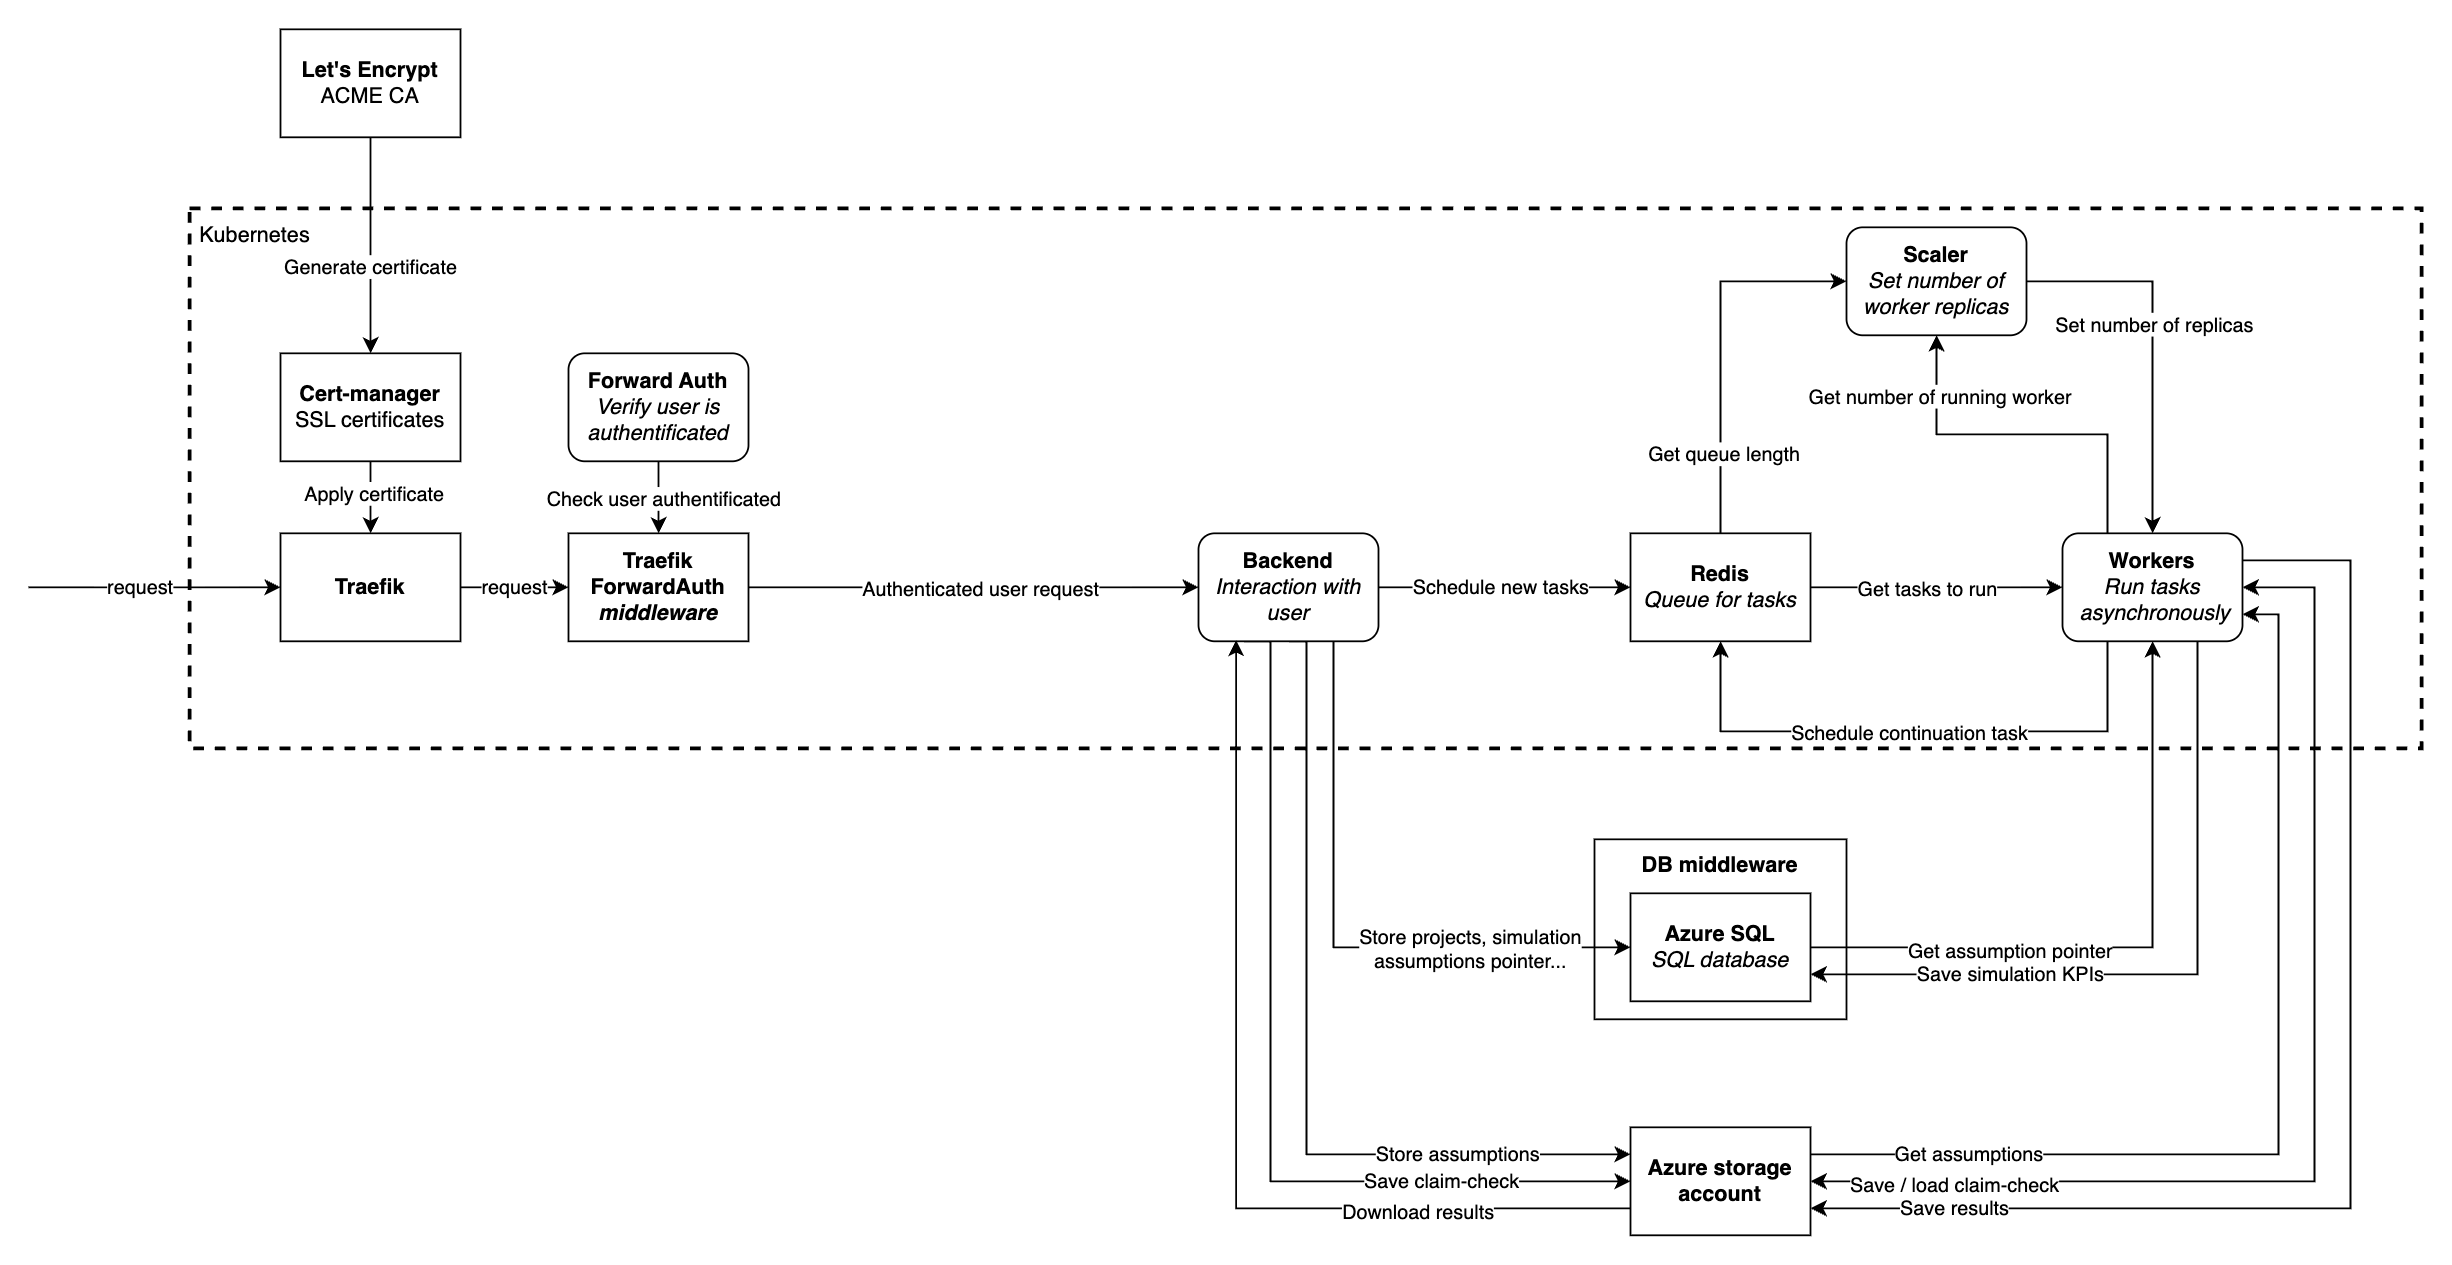
\includegraphics[width=\linewidth]{Figures/deployment_layout.png}
  \caption{Deployment on the managed Kubernetes cluster: ingress and identity edge, backend, broker, autoscaled workers, and data services.}
  \label{fig:deployment-diagram}
\end{figure}

\begin{figure}[H]
  \centering
  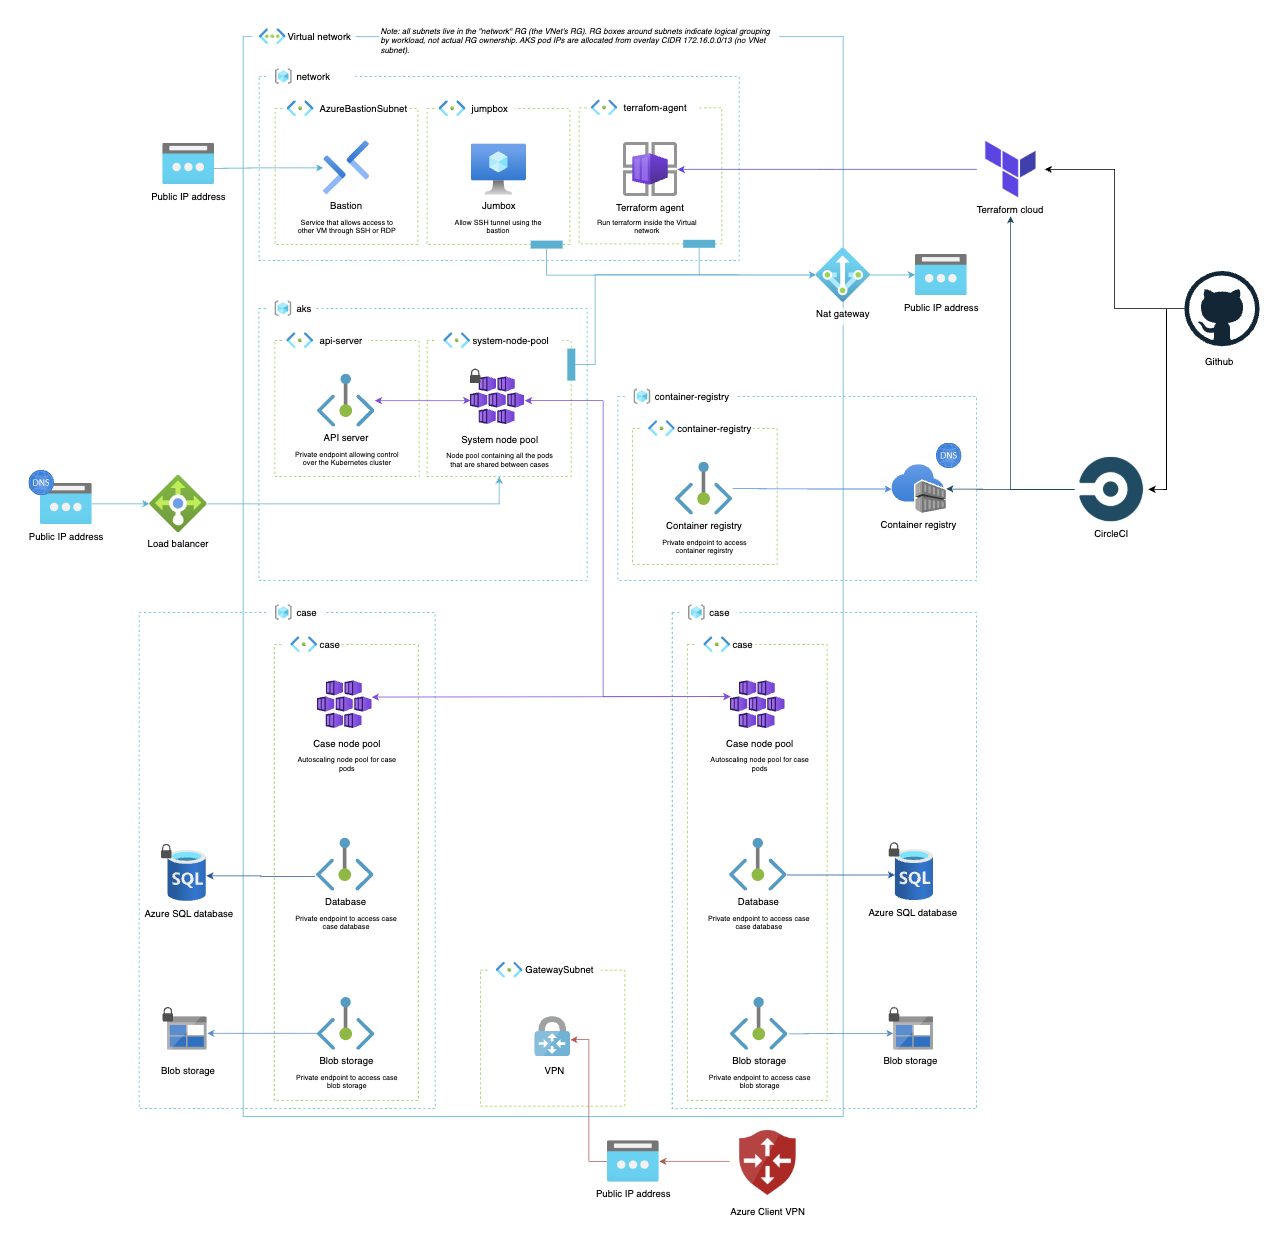
\includegraphics[width=0.82\linewidth]{Figures/azure_infrastructure.png}
  \caption{The underlying cloud infrastructure: private network, controlled admin access, managed node pools, registry, and private-endpoint data services.}
  \label{fig:azure-infra}
\end{figure}

\section{Security and trust boundaries}
\label{sec:trust}

Two trust boundaries structure the design. The first is the \textbf{platform
edge}. External users do not reach application services directly; traffic enters
through a controlled access layer that terminates secure connections and delegates
authentication to the enterprise identity provider through OpenID Connect. The
coordination layer therefore receives requests only after identity has been
established, and uses that identity to enforce access and to attribute activity to
a stable user.

This is a deliberate change from the inherited model. A security assessment of the
inherited identity layer had found weaknesses in the self-hosted setup, where
identity-provider components lived inside the application stack and had to be
patched, configured, and monitored by the product team. The chosen model delegates
sign-in to the enterprise identity provider and forwards only authenticated
traffic to the application (Table~\ref{tab:auth}), reducing the identity surface
owned by the product and aligning it with enterprise governance.

\begin{table}[H]
  \centering
  \begin{tabularx}{\linewidth}{@{}
      >{\raggedright\arraybackslash}p{3.2cm}
      >{\raggedright\arraybackslash}X
      >{\raggedright\arraybackslash}X @{}}
    \toprule
    \textbf{Aspect} & \textbf{Inherited (self-hosted)} & \textbf{Chosen (federated)} \\
    \midrule
    Identity components & Self-hosted providers inside the application stack. &
      Enterprise identity provider through OpenID Connect at the edge. \\
    \addlinespace
    Responsibility & Product team patches, configures, and monitors identity. &
      Identity lifecycle and policy handled by the enterprise. \\
    \addlinespace
    Surface & Larger security and operational surface. & Application receives only
      validated identity information. \\
    \bottomrule
  \end{tabularx}
  \caption{Shift from a self-hosted identity layer to federated enterprise
    authentication.}
  \label{tab:auth}
\end{table}

The second boundary is between \textbf{assistance and mutation}. A language model
may draft a topology change, propose assumptions, or explain results, but it must
not silently commit anything. Every state-changing operation passes through three
gates: a \textbf{typed proposal} (model output becomes a structured payload rather
than free text), \textbf{system validation} (schema, project scope, allowed
fields, and consistency with domain rules), and \textbf{human approval} (the user
explicitly accepts the action before it mutates state or launches computation).
A third boundary sits inside the platform, around the agent runtime itself: the
workers that run language-model reasoning hold no application credentials and
reach project data only through a restricted internal gateway, detailed in
Section~\ref{sec:agent-runtime}. Even if a model were manipulated into attempting
an unauthorized action, it has no direct path to the data, only the narrow,
audited path the gateway allows. The three boundaries are complementary: enterprise
identity controls \emph{who} can act, the approval discipline controls \emph{how}
assisted actions enter the authoritative system, and the runtime boundary controls
\emph{what} the reasoning workers can reach at all.

\section{Data and persistence}
\label{sec:persistence}

The product has several classes of state, and the architecture assigns each to the
storage model that fits it (Table~\ref{tab:storage}). Matching each state class to
a storage responsibility, rather than treating persistence as one undifferentiated
problem, is what keeps the system reliable as it scales.

\begin{table}[H]
  \centering
  \begin{tabularx}{\linewidth}{@{}
      >{\raggedright\arraybackslash}p{3.6cm}
      >{\raggedright\arraybackslash}X @{}}
    \toprule
    \textbf{State type} & \textbf{Storage role and reason} \\
    \midrule
    Canonical project metadata & Structured, queryable store with schema
      discipline, for consistency, auditability, and controlled evolution. \\
    \addlinespace
    Large simulation inputs and outputs & Object storage for big graph payloads,
      result files, and artifacts. \\
    \addlinespace
    Queued simulation work & Dispatch store that decouples interface
      responsiveness from execution and exposes backlog as the scaling signal. \\
    \addlinespace
    Conversational and agentic state & Durable checkpoint store so a multi-step,
      paused interaction can resume exactly where it left off. \\
    \addlinespace
    Agent run dispatch and events & Durable command, lease, and append-only event
      log owned by the agent runtime, so a run is claimed once, recovered after a
      worker loss, and its stream replayed to a reconnecting client. \\
    \addlinespace
    Observability and evaluation & Dedicated records for traces, scores, and
      feedback, kept separate from canonical project data. \\
    \bottomrule
  \end{tabularx}
  \caption{Persistence responsibilities by class of state.}
  \label{tab:storage}
\end{table}

\section{Simulation workflow architecture}
\label{sec:simworkflow}

The simulation workflow is an asynchronous pipeline
(Figure~\ref{fig:sim-sequence}). The user submits a case
through the interface; the coordination layer validates the request, records the
job, and dispatches work to the execution path; dedicated workers run the
deterministic optimization, writing outputs to durable storage; and the interface
retrieves status and results through controlled routes. Long simulations are
processed in chunks so that partial progress can be scheduled without holding the
original request open. In short, a simulation is an authenticated, queued, and
persisted workflow rather than a single blocking call, which is what makes failure
recovery explicit (through job state) rather than tied to a user session.

\begin{figure}[H]
  \centering
  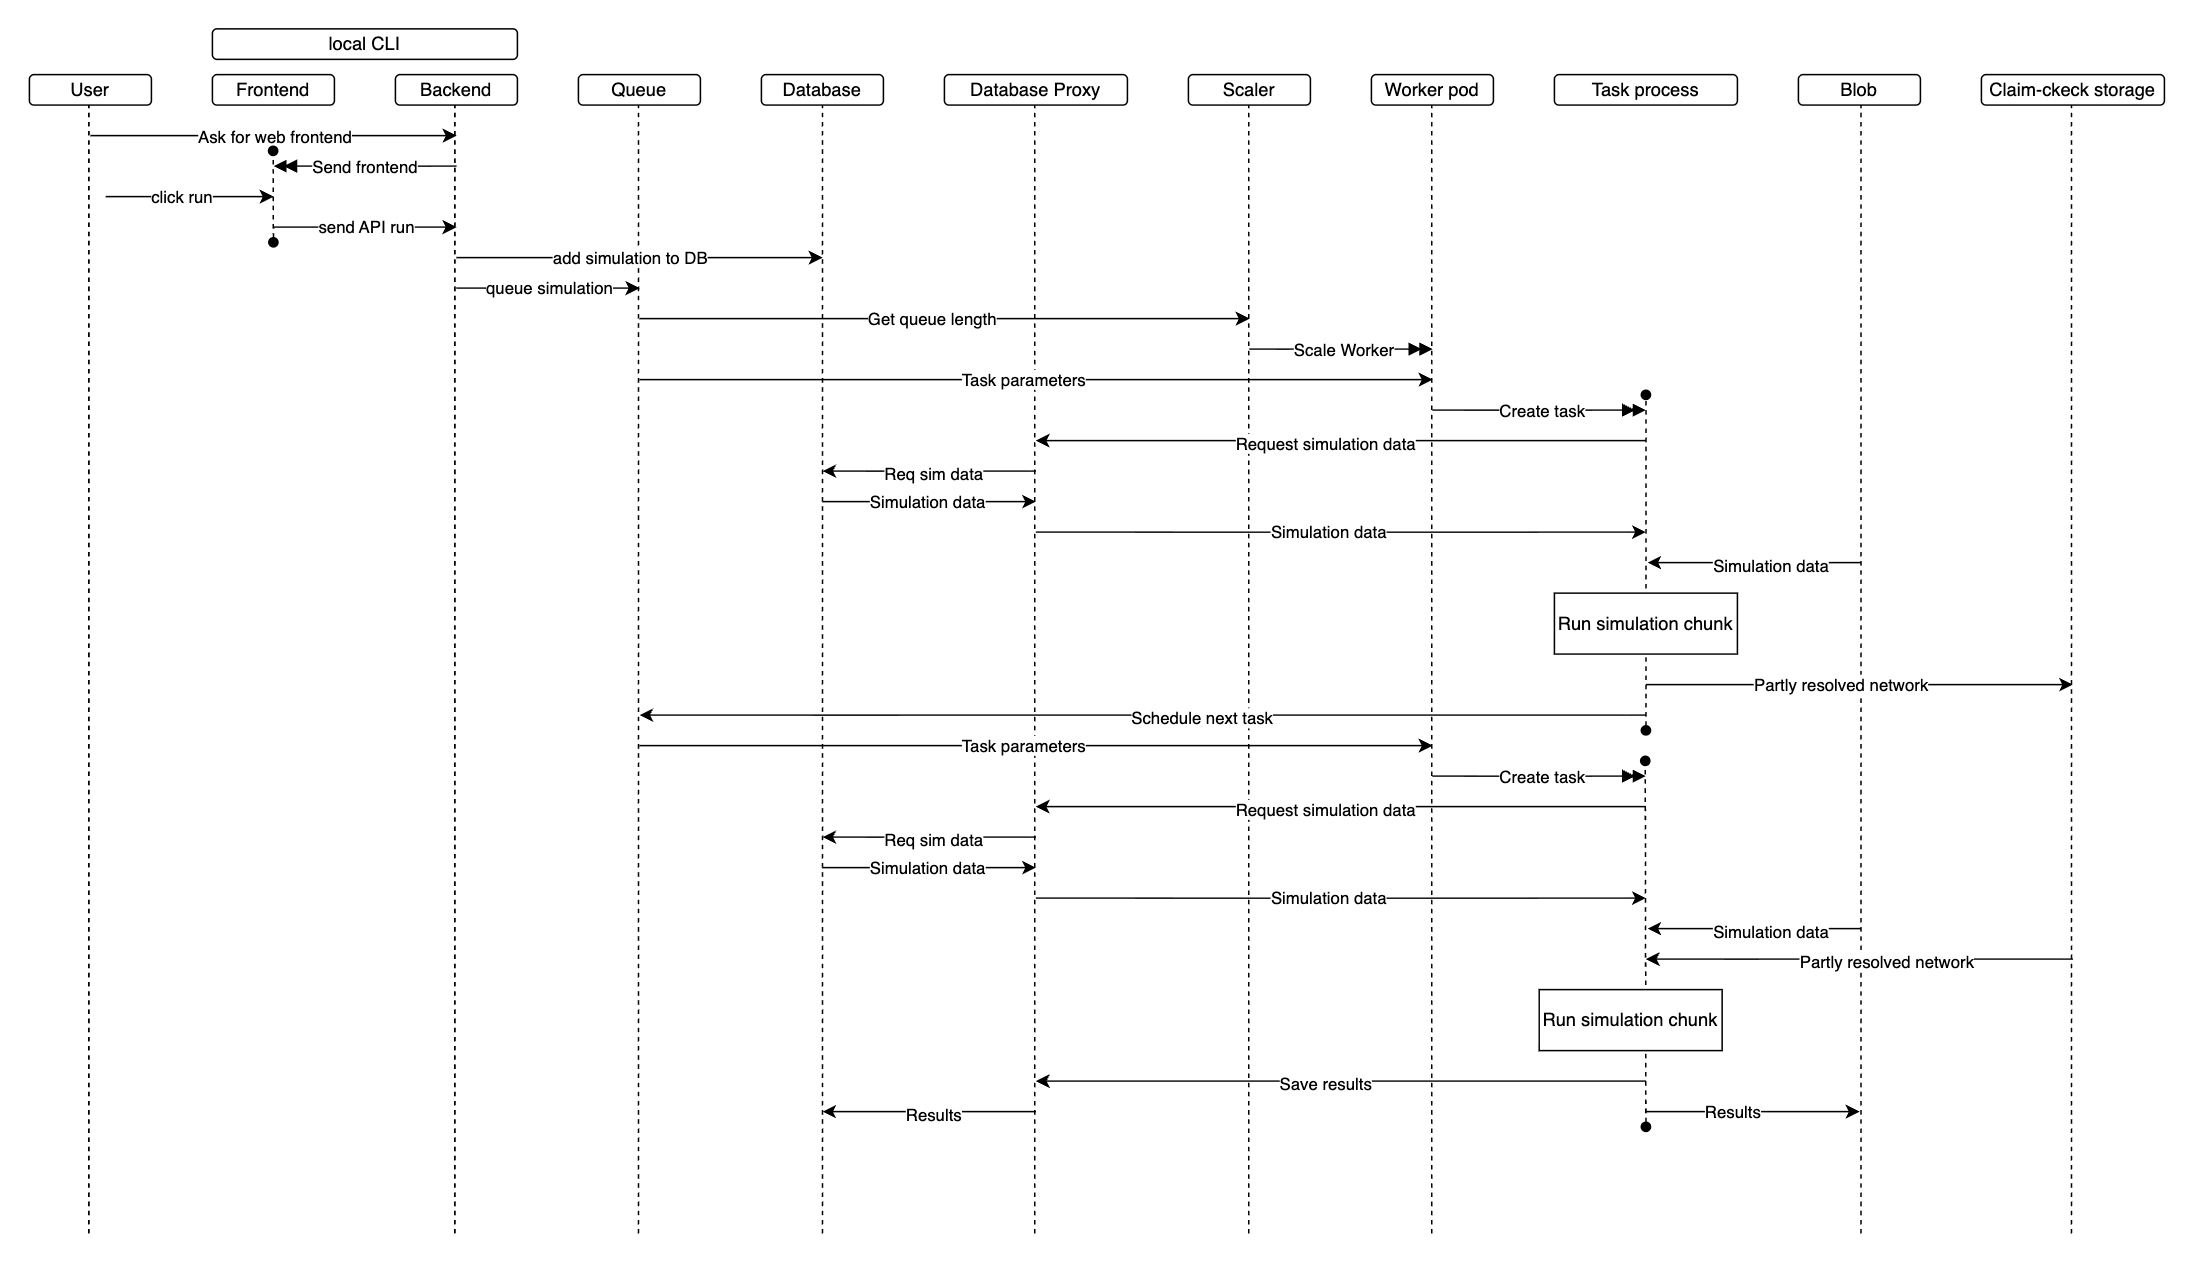
\includegraphics[width=\linewidth]{Figures/sim_sequence.png}
  \caption{End-to-end execution of a simulation run, from enqueue through autoscaled chunked execution to persisted results.}
  \label{fig:sim-sequence}
\end{figure}

A grid search adds one further concern. It can stage hundreds of scenarios at
once, and admitting them all would let a single study monopolize the workers and
would leave the results view empty until the whole sweep finished. The dispatch
path therefore applies \textbf{admission control}: it stages one queued task per
scenario but admits only a bounded number of them in flight per run, releasing the
next as running scenarios reach a terminal state. A set thus \textbf{completes
progressively}, its comparison view filling in as runs finish rather than all at
the end, and the autoscaler follows the admitted backlog rather than provisioning
for the entire sweep at once. The bound is a per-run budget, so the behavior is
inert when the budget is unlimited and adds nothing to a small study, while a large
sweep becomes usable long before it is complete.

\section{Agent runtime and durable execution}
\label{sec:agent-runtime}

The agentic layer does not run inside the application. It is a \textbf{separately
deployed runtime} with its own public boundary, its own workers, its own durable
state, and its own credentials, and the application talks to it over an internal,
versioned interface. The separation is deliberate: language-model work is
long-running, bursty, and probabilistic, so a dedicated runtime keeps its load and
its failures away from the interactive application, while keeping its access to
authoritative data narrow and auditable. This is the second execution plane of
Figure~\ref{fig:two-planes}, and it applies to agent reasoning the same discipline
the simulation plane applies to computation: durable dispatch, conditional
claiming, and checkpointed recovery.

\subsection{Service decomposition}

The runtime is decomposed into focused services with distinct credentials and
scaling (Table~\ref{tab:runtime-services}). An \textbf{Agent API} is the only
public entry point for assisted interaction; the application backend carries no
agent routes and no agent credentials. An \textbf{Agent Control} service owns
durable dispatch and the state transitions of every agent run. \textbf{Interactive}
and \textbf{heavy} worker lanes execute the reasoning graphs, the first tuned for
responsive chat turns and the second for expensive tool work, so a slow task cannot
starve a conversation. Crucially, these workers hold \textbf{no application database
or storage credentials}: every effect they need on project data passes through an
internal \textbf{Tool Gateway}, a strict boundary that exposes only a restricted,
authenticated set of operations under its own principal and is reachable solely
inside the cluster. Bulky housekeeping runs in a separate, isolated executor so
that parsing, model, gateway, and database credentials never accumulate in one
runtime closure.

\begin{table}[H]
  \centering
  \small
  \begin{tabularx}{\linewidth}{@{}>{\raggedright\arraybackslash}p{3.3cm} >{\raggedright\arraybackslash}X@{}}
    \toprule
    \textbf{Service} & \textbf{Responsibility and isolation} \\
    \midrule
    Agent API & The only public entry point for assisted interaction; creates,
      inspects, cancels, resumes, and streams runs. The backend carries no agent
      routes or credentials. \\
    \addlinespace
    Agent Control & Owns durable dispatch and every run's state transitions:
      creation, claim, progress, completion, cancellation, and recovery. \\
    \addlinespace
    Interactive workers & Execute reasoning graphs for responsive chat turns; kept
      warm so latency stays low. \\
    \addlinespace
    Heavy workers & Execute expensive tool and analysis work on a separate lane, so
      a slow task never blocks interactive turns. \\
    \addlinespace
    Tool Gateway & The strict, in-cluster boundary through which workers reach
      project data, under a restricted principal and a narrow authenticated
      interface. \\
    \addlinespace
    State and checkpoint store & Durable run records, leases, append-only events,
      and graph checkpoints, kept separate from application data. \\
    \addlinespace
    Cleanup executor & Isolated pod for bulky housekeeping, so credentials for
      parsing, models, the gateway, and the database never coexist. \\
    \bottomrule
  \end{tabularx}
  \caption{Services of the agent runtime and the isolation of each.}
  \label{tab:runtime-services}
\end{table}

\subsection{Durable dispatch, recovery, and streaming}

An agent run is not a fire-and-forget task; it is a durable command with an
explicit lifecycle (Figure~\ref{fig:agent-runtime}).

\paragraph{Durable dispatch.} When a run is created, its record and a dispatch
entry are written in a single transaction (a transactional outbox); a dispatcher
then publishes the work, and a worker \textbf{claims it conditionally} through a
lease so that exactly one worker owns a run at a time. Because message delivery is
at-least-once, every entry point is idempotent: a redelivered or already-owned run
resumes or becomes a no-op instead of duplicating work or side effects.

\paragraph{Checkpointed recovery.} Each reasoning graph is compiled with a durable
checkpointer and stable run and thread identifiers, and its work is divided at
meaningful boundaries. If a worker is lost mid-run (a deploy, an eviction, a
crash), another resumes from the last checkpoint rather than restarting or dropping
the turn. External effects are made idempotent for the same reason, since a worker
can fail after performing an effect but before recording that it did.

\paragraph{Resumable streaming.} User-visible streaming is backed by a durable
record, not only an ephemeral channel. Each run appends its events with a monotonic
per-run sequence number and then publishes them live; the Agent API replays the
persisted events after a client's cursor and continues with the live stream, so a
browser that reconnects resumes exactly where it left off, losing and duplicating
nothing. The authoritative signal is the final run status; the stream is a
replayable view of it.

\paragraph{Cancellation and bounds.} Cancellation is cooperative: a durable request
is recorded and checked between graph steps and inside long tool loops, rather than
relying on forced process termination. Each turn is bounded by a fixed execution
deadline and a per-turn context limit, so a runaway loop is stopped long before it
can exhaust a worker, and forced termination is the exception rather than the
mechanism.

\begin{figure}[H]
  \centering
  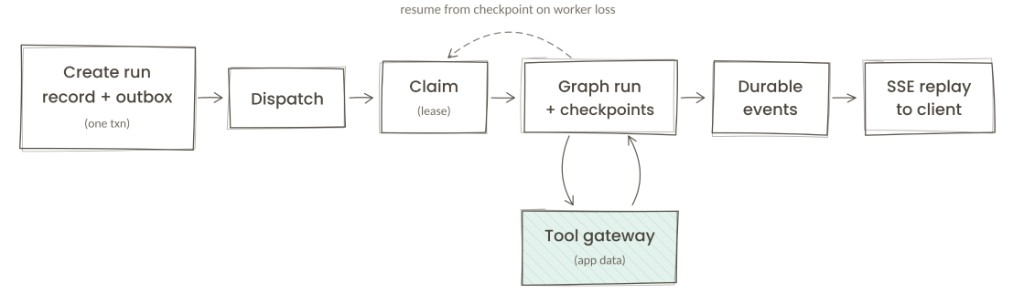
\includegraphics[width=\linewidth]{Figures/agent_runtime_flow.png}
  \caption{Lifecycle of an agent run: dispatched, claimed under a lease, executed
    as a checkpointed graph via the Tool Gateway, and streamed from a replayable
    log.}
  \label{fig:agent-runtime}
\end{figure}

The runtime scales on its own signals and is released and rolled back
independently of the application: interactive workers are kept warm for latency and
heavy workers scale with queue depth, under the same event-driven autoscaling used
for the simulation plane.

\section{The governed multi-agent layer}
\label{sec:agentic}

The agentic layer sits above the existing product as an assistant, not a
replacement. Its role is to reduce the friction of complex analytical workflows:
describing a topology, identifying missing assumptions, preparing scenario
variants, interpreting results, and guiding the user toward the next action.
Figure~\ref{fig:agentic-arch} shows the governing idea: reads execute immediately,
writes become approval-gated proposals, and the deterministic engine remains the
numerical authority.

\begin{figure}[H]
  \centering
  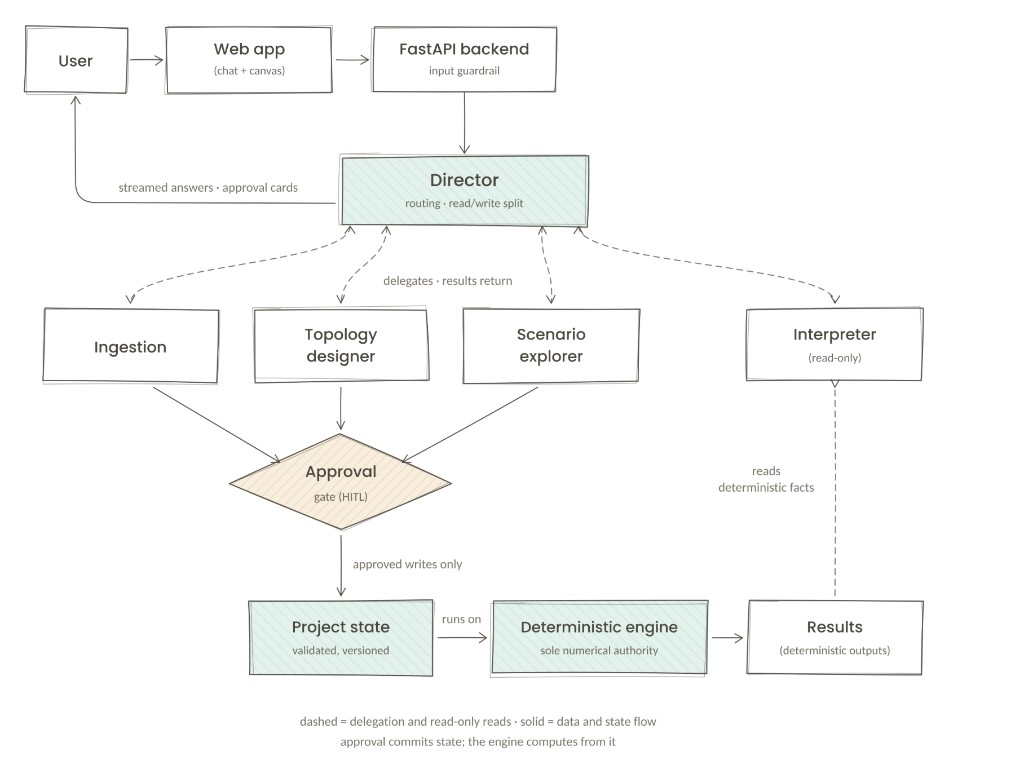
\includegraphics[width=0.92\linewidth]{Figures/agentic_flow.png}
  \caption{Governed multi-agent architecture: the Director routes each request,
    specialists propose, approved writes commit validated project state, and the
    deterministic engine computes all results (the interpreter is read-only).}
  \label{fig:agentic-arch}
\end{figure}

\subsection{Agent topology}

The agentic layer decomposes into controlled roles that form a governed hierarchy
around a single conversational entry point, rather than a set of independent
chatbots (Table~\ref{tab:agents}). The Director delegates specialist work to
focused flows, receives structured results, and turns state-changing
recommendations into approval cards. Figure~\ref{fig:agent-hierarchy}
summarizes this hierarchy and the boundary of each role.

\begin{figure}[H]
  \centering
  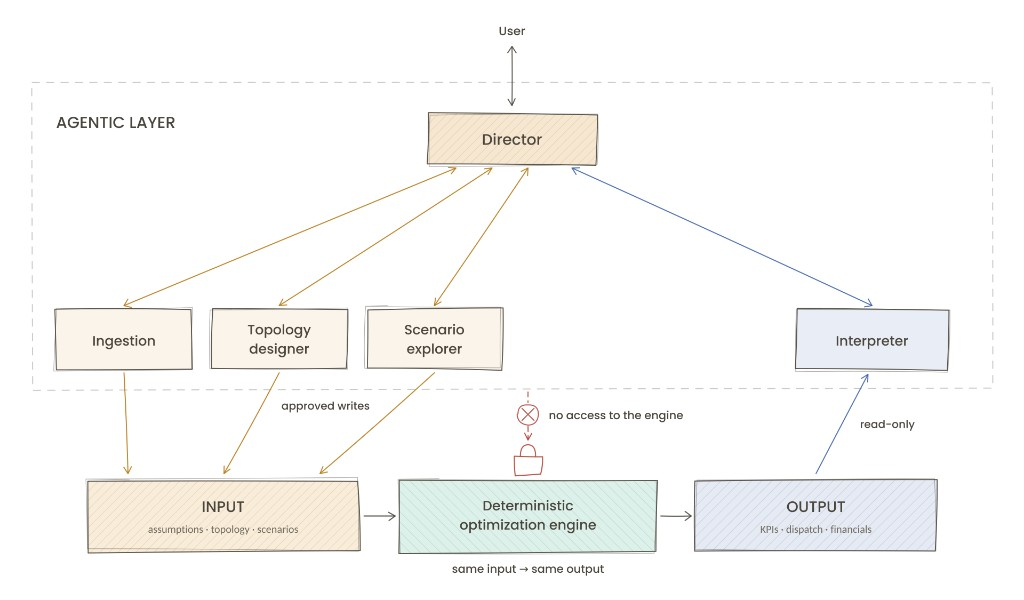
\includegraphics[width=0.95\linewidth]{Figures/agents_io_boundary.png}
  \caption{The Director and its specialists act only on the engine's inputs
    and outputs: writes are approved, reads are read-only, and the
    deterministic engine itself is never touched.}
  \label{fig:agent-hierarchy}
\end{figure}


\begin{table}[H]
  \centering
  \begin{tabularx}{\linewidth}{@{}
      >{\raggedright\arraybackslash}p{3.4cm}
      >{\raggedright\arraybackslash}X @{}}
    \toprule
    \textbf{Role family} & \textbf{Main roles and boundary} \\
    \midrule
    Conversation and approval & Director, bounded operations, proposal creation,
      pending-approval state. A single entry point: read-only operations answer
      directly, while write intent becomes an approval card before execution. \\
    \addlinespace
    Structure and ingestion & Topology Designer and Ingestion Agent. Produce draft
      topology proposals or staged assumption-file previews; project mutation
      remains approval-gated. \\
    \addlinespace
    Scenario exploration & Scenario Explorer with a scoping Analyst and four axis
      agents. Runs bounded parameter exploration and returns approval-ready canvas
      operations. \\
    \addlinespace
    Result interpretation & Interpreter agent and result-inspection
      operations. A read-only explanation loop that returns narrative and cards
      and never writes state. \\
    \bottomrule
  \end{tabularx}
  \caption{Agentic roles and their boundaries.}
  \label{tab:agents}
\end{table}

\subsection{Delegation and flow-level design}

Each flow is a controlled reasoning process with a defined state, explicit steps,
conditional routes, and local retries, rather than a single prompt. A typical turn
follows a controlled path: the Director grounds the request in the active project,
page, and conversation, answers directly or with a read-only operation when it
can, and otherwise delegates to the appropriate specialist.

\paragraph{Director.} The root reasoning flow exposed to the user. The current
message and session context enter a reason-and-act loop; the assistant either
answers or requests a bounded tool, tool results return to the reasoning path, and
the loop continues until a final answer or a proposal is emitted. Control logic
around the loop injects the active project and page, suppresses duplicate expensive
calls within a turn, and intercepts proposal-producing actions before they can be
narrated as already executed.

\paragraph{Topology designer.} A specialist flow for structural work. It resolves
the active canvas, saved topology, or previous proposal; diagnoses the task;
gathers evidence through scoped rule injection (the general rules plus the rules
for the one classified project type) and few-shot retrieval of structurally
similar library designs; generates candidate structures; compiles the chosen one
into a patch; and validates it against schema and domain rules. A design that fails
validation is not silently repaired: the flow attempts deterministic repair or
guided re-planning, and otherwise blocks with the failing evidence. Even a
successful path stores only a draft proposal.

\paragraph{Ingestion agent.} A staged, mostly deterministic pipeline that handles
uploaded assumption files as a batch. It loads the batch, parses and classifies
each file (using the model only where deterministic classification is not
confident), places recognized records into assumption slots, detects conflicts
with existing project data, stages the result, and returns a reviewable
data-quality report. The output is a preview for approval, not an immediate
mutation.

\paragraph{Scenario explorer and axis agents.} The most nested flow. A scoping
Analyst first checks that the request contains enough information (location,
activation year, plant scale, objective) and short-circuits with a clarifying
question if not. When scope is sufficient, four parallel axis agents propose sweep
values in their own domain, the technical axis for asset sizing, the commercial
axis for off-take and purchase terms, the financial axis for cost-of-capital and
tax, and the external axis for market prices and macro inputs. The Analyst
reconciles them, drops references that do not resolve against the live topology,
and returns a single validated set of canvas operations for one approval.

\subsection{Design of the result-interpretation agent}
\label{sec:interp-design}

The result-interpretation agent realizes result interpretation (F4). It explains a completed
simulation population in natural language, and its design is dominated by one
demand: it must be helpful without ever becoming a source of numerical truth.

\paragraph{A read-only reason-and-act loop.} The interpreter is not a separate
chatbot: the Director exposes it as a \textbf{single tool}, and once that tool is
called the Director suppresses its own narration for the turn, so the
interpreter's grounded voice is the only one the user hears. It runs on its
\textbf{own reasoning-capable model}, distinct from the Director's, as a small
state machine that alternates between reasoning about the user's question and
calling a read-only tool to retrieve evidence, then reasoning again over what it
retrieved, until it can answer (Figure~\ref{fig:interp-flow}). The loop is
\textbf{bounded}, by a fixed number of tool rounds and a hard timeout, so it always
terminates. Because its tools never mutate state, the interpreter needs no approval
gate, which is what allows it to answer immediately while the writing agents remain
gated.

\begin{figure}[H]
  \centering
  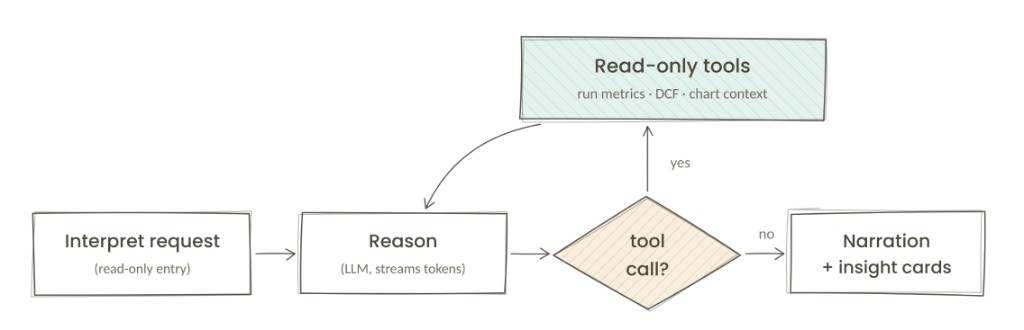
\includegraphics[width=\linewidth]{Figures/interp_flow_light.png}
  \caption{The interpreter as a read-only reason-and-act loop over deterministic
    tools, with bounded tool rounds.}
  \label{fig:interp-flow}
\end{figure}

\paragraph{Grounded, injection-resistant tool contracts.} The interpreter reasons over
facts obtained from a small set of read-only tools with structured outputs: run
metrics, discounted-cash-flow and income-statement breakdowns, sensitivities, and
chart context. The persona prompt forbids the model from computing figures itself;
every quantitative statement must cite a value returned by a tool. This is the
concrete mechanism behind the groundedness requirement (\hyperlink{nf:groundedness}{NF2}): the model organizes
and phrases evidence, but the evidence comes from the deterministic engine, so
there are no invented numbers. Decisively, these tools do not re-implement any
analysis: they call the \textbf{same pure, unit-tested functions that compute the
on-screen charts}, so the figures an explanation cites cannot differ from the
numbers the user sees.
Table~\ref{tab:interp-tools} lists the read-only tools available to the
interpreter. A useful illustration is restraint: asked to read a trend from a
scatter with a single point, the interpreter states that no relationship can be
inferred rather than fabricating one.

\begin{table}[H]
  \centering
  \small
  \begin{tabularx}{\linewidth}{@{}>{\raggedright\arraybackslash}p{4.1cm} >{\raggedright\arraybackslash}X@{}}
    \toprule
    \textbf{Read-only tool} & \textbf{What it reads} \\
    \midrule
    Result summary & The indicators available across the runs of a study. \\
    Best runs & A ranking of runs by a chosen indicator. \\
    Single-run operational read & One run's operating story (storage state, market
      trades, prices, peaks), and renders its chart. \\
    Additional chart & An extra chart panel as the narrative develops. \\
    Run configuration & The design levers of a run (asset sizes, cost of capital,
      market setup). \\
    Discounted cash flow & The per-year cash-flow table (revenue, costs, tax, net
      and cumulative flow). \\
    Scatter read & The scatter of one metric against another that the user is
      viewing. \\
    Axis-pair suggestions & Informative pairs of metrics to plot. \\
    Run comparison & The differences between two runs. \\
    Parameter suggestions & Which levers move a chosen indicator. \\
    \bottomrule
  \end{tabularx}
  \caption{The interpreter's read-only tools, each returning facts from the same analytics that produce the charts.}
  \label{tab:interp-tools}
\end{table}

\paragraph{Streaming and bounded turns.} The interpreter streams its narration
token by token so that the user receives feedback immediately, and returns a set of
\textbf{insight cards} alongside the prose, optionally embedding the chart the
explanation refers to. Each interpretation runs as a \textbf{fresh, stateless
turn}: no prior conversation enters it, only the analyst persona and the on-screen
question, and only compact, pre-aggregated facts reach the model, each truncated to
a hard ceiling. The turn therefore stays small by construction and never approaches
the context limit, which keeps it fast and cheap as well as grounded.

\subsection{Graph control principles}

Across all these flows, the same control principles apply: \textbf{typed state}
(each flow carries an explicit schema), \textbf{conditional routing} (blocking
conditions, missing inputs, and repair paths are explicit routes),
\textbf{local retries} (transient or malformed outputs are retried inside the flow
that owns the failure), \textbf{progress streaming} (long flows emit progress
events so the interface can show which lane is running), and \textbf{deterministic
final authority} (even a successful assisted flow only prepares inputs or scenario
definitions). The approval gate (F6) is thus part of the architecture, not a
user-interface detail: the model may recommend, the system validates, the user
approves, and only then may state change.

\section{Design of the visualization layer}
\label{sec:viz-design}

The visualization layer realizes results visualization (F5) and is the
surface on which interpretation is offered. It is built as a set of components over
the deterministic outputs, organized so that a user moves naturally from comparing
a whole population of runs, to reading one run in depth, to asking for an
explanation of exactly what is on screen.

\paragraph{Two views.} The results are presented through two tabs. A
\textbf{library} view manages the runs of the
selected studies: it lists every
simulation with its live status, supports search, download, and cancellation, and
refreshes while work is still in progress. A \textbf{chart} view is the analytical
core, laid out top to bottom as controls, a comparison scatter, and a per-run
dashboard. The realized views are shown in Chapter~\ref{chap:implementation}
(Figures~\ref{fig:impl-library} and~\ref{fig:impl-scatter}).

\paragraph{Comparing runs: the scatter.} The central element is a \textbf{scatter
with selectable axes}: one point per simulation
across the selected studies,
positioned by any pair of financial or operational indicators, which makes
trade-offs (for example capital cost against return) and standout runs immediately
visible. The axis choices are not a flat list. They are grouped into scanned
inputs, indicator outputs, constant quantities, and pairs that are incompatible
with the current axis, and a pair is offered only when the two metrics actually
share data across the selected runs, which prevents empty or degenerate plots.
Hovering a point reveals its key metrics and asset configuration; clicking it
selects the run and opens its dashboard; and a box drawn on the plot zooms into a
region, with each study drawn in its own marker and color so several sets can be
compared at once.

\paragraph{Reading one run: the operational dashboard.} Selecting a point opens a
dashboard that tells that run's \textbf{operational money story} across six panels
(Table~\ref{tab:viz-panels}; realized in
Figure~\ref{fig:impl-dashboard}), governed by a time-filter sidebar that sets the scope
and granularity, from a monthly overview down to a scoped hourly window. Panels
appear only for the assets a run actually contains, so an islanded plant or a plant
without storage simply omits the panels that do not apply.


\begin{table}[H]
  \centering
  \small
  \begin{tabularx}{\linewidth}{@{}>{\raggedright\arraybackslash}p{4.2cm} >{\raggedright\arraybackslash}X@{}}
    \toprule
    \textbf{Panel} & \textbf{What it shows} \\
    \midrule
    Effective revenue & Revenue over time, with cumulative revenue on a second
      axis. \\
    Market imports and exports & Quantity bought and sold per market over time, with
      price on a second axis; a market picker and quantity, revenue, or price
      modes. \\
    Energy mix & Generation over time by source, for the sources present in the
      topology. \\
    Battery state of charge & When the battery charges and discharges over time. \\
    Solar load factor & Average solar utilization over time. \\
    Wind load factor & Average wind utilization over time. \\
    \bottomrule
  \end{tabularx}
  \caption{The per-run operational dashboard: the six panels of a run's operational money story.}
  \label{tab:viz-panels}
\end{table}

\paragraph{The financial view.} Alongside the operational panels, a dedicated
component renders the \textbf{discounted-cash-flow and income statement} as a
grouped, expandable table (years by line items) with drill-down to per-asset and
per-market components, amortization and debt groups, reconciliation, payback
highlighting, sign-aware formatting, and hover-for-exact-figure
(Figure~\ref{fig:viz-financial}). It turns a dense
financial statement into something a non-specialist can navigate and audit.

\begin{figure}[H]
  \centering
  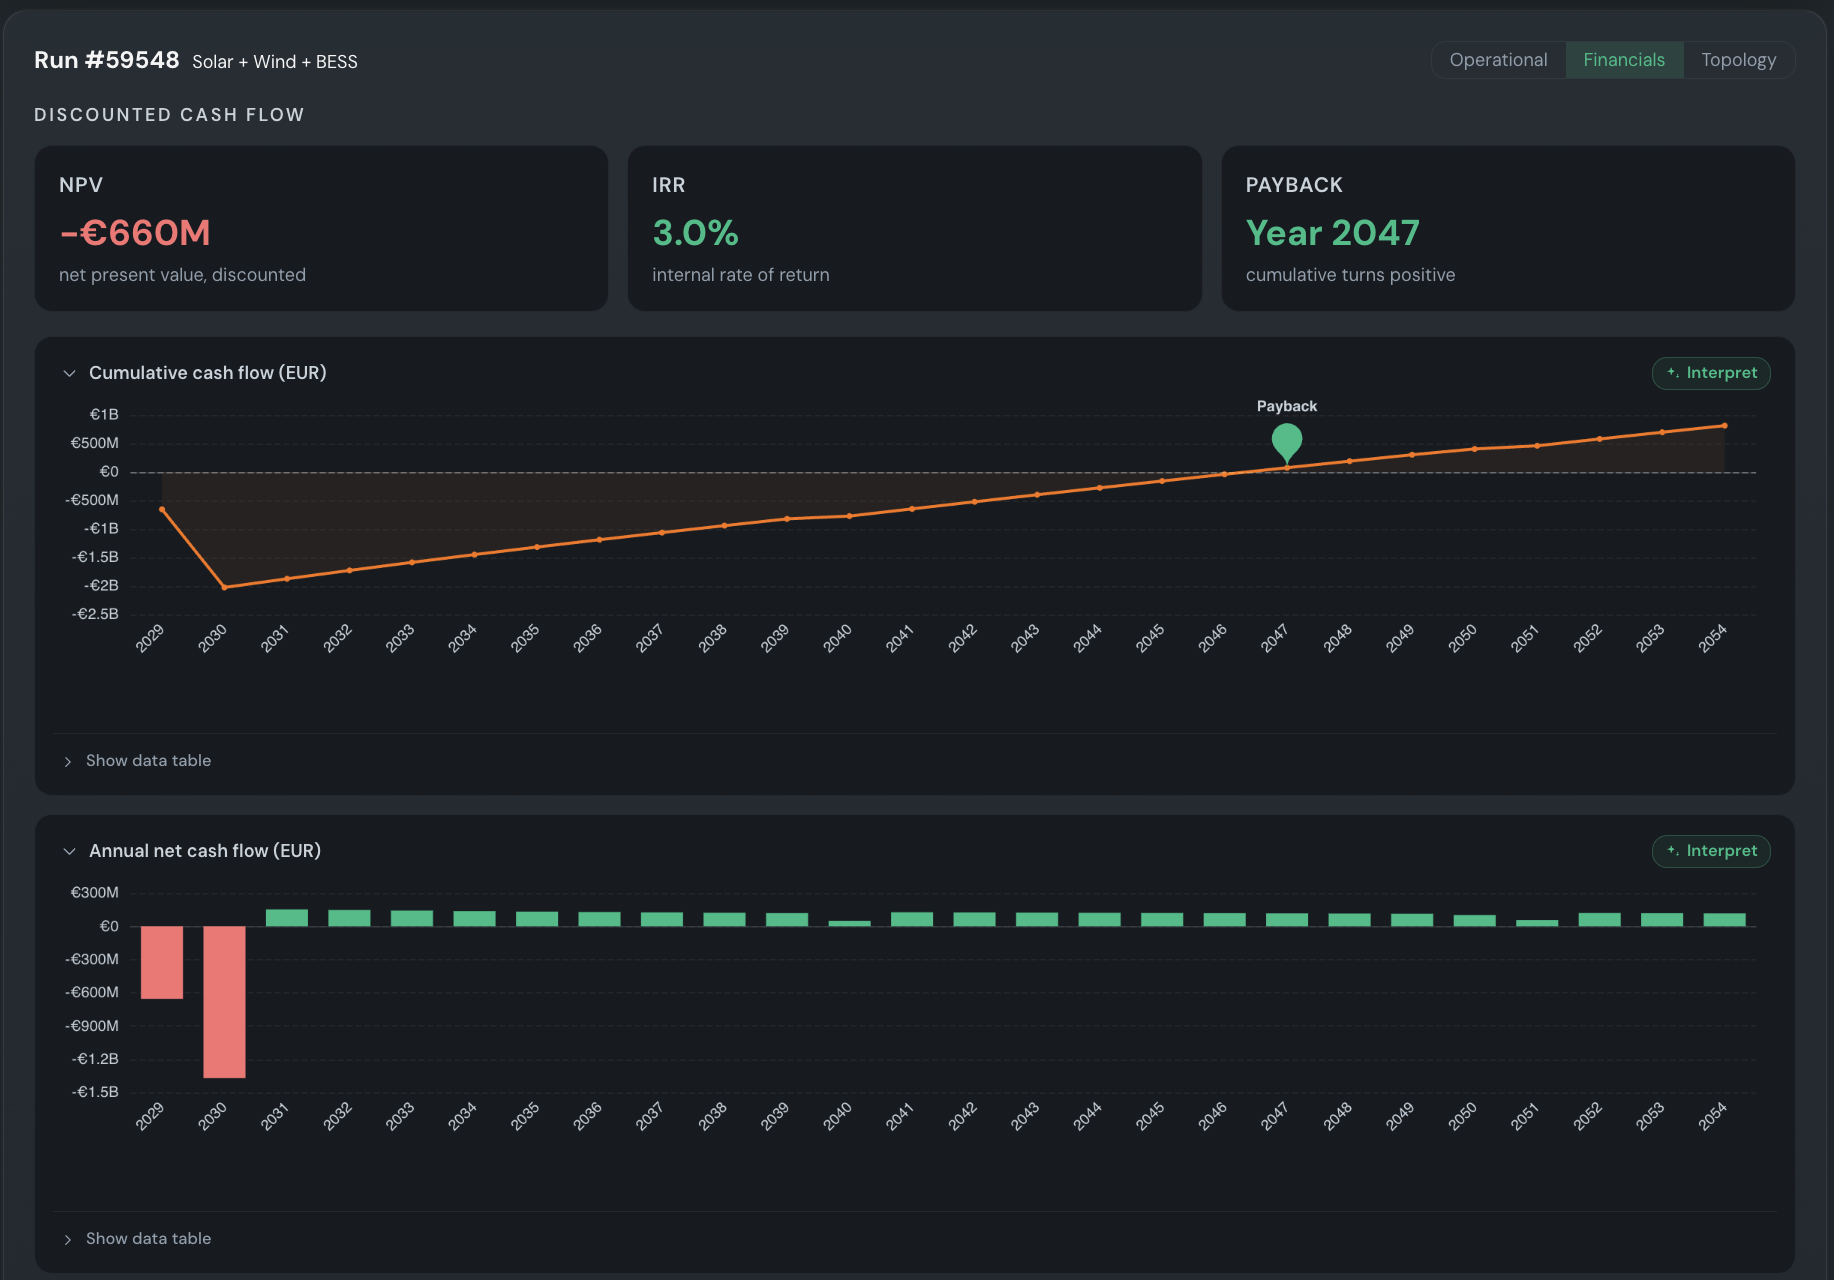
\includegraphics[width=0.8\linewidth]{Figures/05.png}
  \caption{The financial view of a run: headline indicators (NPV, IRR, payback)
    above the cumulative and annual discounted-cash-flow charts.}
  \label{fig:viz-financial}
\end{figure}

\paragraph{Interpret on demand.} Finally, each chart exposes an
\textbf{interpret-on-demand} action that attaches a grounded, streamed explanation
from the interpreter to the exact view the user is looking at, passing along the
run, the time window, the granularity, and any active filters. Because both the
charts and the interpreter read the same deterministic analytics, the figures the
explanation cites cannot differ from the figures the chart plots. This ties
visualization and interpretation
together while keeping the boundary between shown data and generated commentary
clear; the realized interface is shown in Chapter~\ref{chap:implementation}
(Figure~\ref{fig:impl-interp}).

\section{Design of the evaluation harness}
\label{sec:eval-design}

Because the assisted capabilities rely on a language model, their quality has to be
measured rather than assumed (\hyperlink{nf:eval}{NF6}). The evaluation harness
(F7) turns that requirement into a concrete mechanism.

\paragraph{An independent judge.} Interpretations are free text, so they are scored
by an independent \textbf{judge model} on four dimensions, each from 0 to 1
(Table~\ref{tab:judge}), against a rubric distilled from the product's own
financial and commercial expert prompts, so the grading reflects real domain rules.
The judge is a single call made \emph{outside} the interpreter loop: a grading
hiccup can therefore never break the user's answer, and an independent grader is
more trustworthy than a model grading itself. Each case is scored more than once and
aggregated, since a single judgement is noisy. The four scores as they appear on a
real trace are shown in Chapter~\ref{chap:implementation}
(Figure~\ref{fig:impl-judge-scores}).

\begin{table}[H]
  \centering
  \small
  \begin{tabularx}{\linewidth}{@{}>{\raggedright\arraybackslash}p{3.7cm} >{\raggedright\arraybackslash}X@{}}
    \toprule
    \textbf{Dimension} & \textbf{What it checks} \\
    \midrule
    Groundedness & Every figure traces back to a tool fact, with no invented
      numbers. The most checkable and most trustworthy dimension. \\
    Financial soundness & Cost-of-capital and discounting use, cash-flow
      consistency, depreciation and tax, currency consistency. \\
    Commercial soundness & Realistic price bands for the market setup; an islanded
      plant treated differently from a traded one. \\
    Operational coherence & A causal charge, discharge, and market story that
      actually hangs together. \\
    \bottomrule
  \end{tabularx}
  \caption{The rubric the judge scores each interpretation against.}
  \label{tab:judge}
\end{table}

\paragraph{Online and offline.} The same judge runs in two modes. \textbf{Online},
after each interpretation it fires in the background (sampled, so cost can be dialed
down) and writes the four scores onto that turn's trace, which makes quality visible
live without delaying the user. \textbf{Offline}, it runs over a curated dataset
through a harness, so a change to the interpreter's prompt or the expert rubrics is
validated by re-running and comparing the score deltas across versions on the same
cases.



\paragraph{A closing feedback loop.} Users rate each answer with a thumbs signal
that is recorded as a score; nightly jobs promote weak turns into the review
dataset and re-run the evaluation. Poor answers are thus surfaced and become the
next round of prompt work, so the system does not only explain results, it
\textbf{measures and improves its own explanations} over time
(Figure~\ref{fig:eval-loop}).

\paragraph{Structural fidelity.} A complementary method covers the components that
produce a graph, notably the topology designer: fidelity is measured against
curated golden references using the graph edit distance, which captures structural
similarity that string comparison cannot. Together, the free-text judge and the
structural metric cover both kinds of assisted output the platform produces.

\begin{figure}[H]
  \centering
  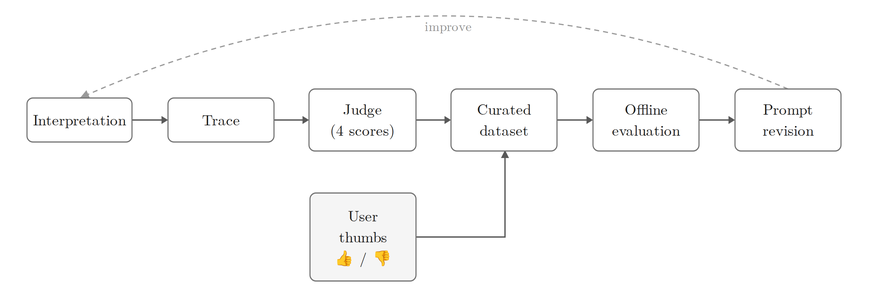
\includegraphics[width=\linewidth]{Figures/11.png}
  \caption{The evaluation loop: each interpretation is traced and judged on four dimensions, with weak turns re-scored offline.}
  \label{fig:eval-loop}
\end{figure}

\section{Interaction design}
\label{sec:interaction}

The interface must support two kinds of work: conventional analytical workflows
(project navigation, topology editing, scenario configuration, result exploration)
and conversational assistance (streamed responses, proposal cards, approval and
rejection controls, and validation feedback). It is therefore treated as a coherent
design system rather than a collection of unrelated screens: the same primitives,
buttons, forms, tables, dialogs, status badges, and cards, behave consistently
whether the user is editing manually or responding to an assistant proposal. This
consistency is also a trust decision, because it lets users reliably distinguish
draft, pending, approved, and committed states, which makes the governance of the
agentic layer visible rather than hidden.

\section{Observability and operational architecture}
\label{sec:observability}

The architecture requires operational controls around the runtime, split between
the application layer and the platform layer. Observability records every model
call, tool invocation, latency, cost, and evaluator score, so that a visible answer
can be traced back to the exact reasoning and evidence that produced it, and so
that assisted behavior can be debugged and costed. Because the agent runtime is a
separate service, a single trace is propagated across the boundary, from the
application request through the Agent API, the worker, the reasoning graph, and its
model and tool calls, so that even a cross-service answer can be followed end to
end.

Beyond tracing, the platform includes an \textbf{operational monitoring loop}
around a \textbf{read-only assessment agent}. On a schedule, a runner performs
deterministic health checks first, public and internal reachability, read-only API
checks, and a synthetic end-to-end journey in a temporary test project, and then
asks the read-only assessment agent for an evidence-based status. The agent can
inspect resources, logs, traces, and route health, but its toolset excludes any
mutation; the runner, not the agent, owns the few bounded side effects (creating
and deleting the synthetic test project, storing the report, and sending
notifications). The output is a compact status, GREEN, YELLOW, or RED, with
evidence and suspected causes; the delivered report is shown in
Chapter~\ref{chap:implementation} (Figure~\ref{fig:impl-qa}). Keeping the
assessment agent read-only mirrors, at
the platform level, the same assistance-versus-authority principle that governs the
product agents.

\section{Architecture summary}
\label{sec:arch-summary}

Table~\ref{tab:responsibilities} summarizes the responsibilities and trust
principle of each layer. The deterministic core remains authoritative; the platform
makes it secure and deployable; the interaction layer makes it usable; the execution
and persistence design make it scalable; observability and monitoring make its
behavior inspectable; and the agentic layer makes complex workflows easier without
weakening auditability.

\begin{table}[!ht]
  \centering
  \begin{tabularx}{\linewidth}{@{}
      >{\raggedright\arraybackslash}p{3.1cm}
      >{\raggedright\arraybackslash}X
      >{\raggedright\arraybackslash}p{4.2cm} @{}}
    \toprule
    \textbf{Layer} & \textbf{Primary responsibility} & \textbf{Trust principle} \\
    \midrule
    Presentation & Make project, topology, scenario, result, and approval
      workflows usable. & Show state clearly; never hide proposed mutations. \\
    \addlinespace
    Coordination & Validate requests, serve state, coordinate persistence and
      dispatch. & Centralize state transitions behind typed contracts. \\
    \addlinespace
    Deterministic execution & Run optimization workloads and produce auditable
      numerical outputs. & Keep computation reproducible and independent of the
      language model. \\
    \addlinespace
    Persistence & Store canonical data, large artifacts, dispatch state, and
      checkpoints. & Match storage to state type and recovery need. \\
    \addlinespace
    Agent runtime & Assist through routing, specialists, and interpretation, on a
      separate, durably dispatched execution plane. & Hold no direct data access;
      propose under constraints; mutate only after validation and approval. \\
    \addlinespace
    Platform & Provide managed runtime, authenticated access, and observability. &
      Make delivery repeatable, auditable, and enterprise-aligned. \\
    \bottomrule
  \end{tabularx}
  \caption{System responsibilities and trust principles by layer.}
  \label{tab:responsibilities}
\end{table}

\section*{Conclusion}

This chapter presented the full architecture around the deterministic core: the
architectural objectives, the logical decomposition and its graph views, the
runtime and cloud deployment model, the security and identity boundaries, the
persistence and simulation workflow, and the governed multi-agent layer with each
of its agents. It detailed the design of the read-only interpreter, the
visualization layer, and the evaluation harness within that complete system, and
it showed how every layer
upholds the principle that assistance never becomes numerical authority. The next
chapter turns this design into a concrete implementation and reports its
evaluation.


\chapter{Implementation and Evaluation}
\label{chap:implementation}

\section*{Introduction}

Chapter~\ref{chap:design} described the design and the boundaries between the
deterministic optimizer, the application platform, and the governed agentic layer.
This chapter moves from design to implementation. It first presents the main
technologies used across the platform. It then documents the implemented product
through a screenshot showcase that follows the user journey, from product entry to
result interpretation, and reports the surrounding platform and operations work
(enterprise access, delivery, monitoring, and observability). The evaluation of the
assisted behavior is reported last, before the chapter conclusion.

\section{Main technologies}
\label{sec:tech}

The implementation reused the existing Energy Transition Optimizer foundation and
extended it with a governed agentic layer, a restored platform, and an
observability and evaluation stack. The stack was therefore not a greenfield
choice but a pragmatic combination of the technologies already present in the
product and those required to restore, secure, deploy, and extend it. This section
covers the main technologies only; supporting libraries are treated as
implementation details where they become relevant.

\subsection{Frontend technologies}

\paragraph{Next.js.} Next.js provides the routing, build model, and React-based
foundation behind the product workspace, supporting project navigation, topology
editing, assumption ingestion, simulation review, and the agentic chat interface.
\begin{center}
\includegraphics[height=1.4cm]{Figures/tech/nextjs.png}\end{center}

\paragraph{TypeScript.} TypeScript is the main frontend language; typing the API
contracts, component properties, application state, and generated client models
makes client-side development safer around structured domain objects such as
topologies, approval cards, and streamed agentic events.
\begin{center}
\includegraphics[height=1.4cm]{Figures/tech/typescript.png}\end{center}

\subsection{Backend and deterministic execution}

\paragraph{Python.} Python is the main backend and computation language, shared by
the API service, the deterministic optimization engine, background workers, and the
agentic implementation, which keeps product, solver, and agent logic close to the
same domain model.
\begin{center}
\includegraphics[height=1.4cm]{Figures/tech/python.png}\end{center}

\paragraph{FastAPI.} FastAPI exposes the application API for projects, ingestion,
simulations, agentic sessions, approvals, and health checks, with a typed
request-response model that matters when agentic proposals must be validated before
reaching application state.
\begin{center}
\includegraphics[height=1.4cm]{Figures/tech/fastapi.png}\end{center}

\paragraph{OR-Tools.} OR-Tools is the optimization technology behind the
deterministic core, responsible for the constrained scheduling that produces
operational and financial outputs; the project preserved this deterministic
authority rather than replacing it with language-model reasoning.
\begin{center}
\includegraphics[height=1.4cm]{Figures/tech/ortools.png}\end{center}

\paragraph{Celery.} Celery runs long simulations as asynchronous background work,
so the API stays responsive while deterministic computation runs outside the
request-response path; its workers are treated as a dedicated execution layer.
\begin{center}
\includegraphics[height=1.4cm]{Figures/tech/celery.png}\end{center}

\subsection{Agentic technologies}

\paragraph{LangChain and LangGraph.} LangChain provides the agent and tool-calling
foundation used by the Director, while LangGraph structures specialist workflows as
explicit state graphs, supporting bounded delegation, streaming, resumable state,
and approval-gated interactions rather than an unstructured chatbot.
\begin{center}
\includegraphics[height=1.4cm]{Figures/tech/langchain.png}\end{center}

\paragraph{OpenAI-compatible models.} OpenAI-compatible chat models provide the
reasoning capability of the agentic layer; their authority is intentionally
constrained, since model outputs become structured proposals rather than direct
mutations of project state.
\begin{center}
\includegraphics[height=1.4cm]{Figures/tech/openai.png}\end{center}

\paragraph{Langfuse.} Langfuse is the observability platform for the agentic layer,
recording model calls, tool trajectories, traces, evaluator scores, and prompt
versions so that assisted behavior can be inspected after execution.
\begin{center}
\includegraphics[height=1.4cm]{Figures/tech/langfuse.png}\end{center}

\subsection{Persistence and messaging}

\paragraph{PostgreSQL.} PostgreSQL provides durable checkpointing for the agentic
layer, keeping conversational execution state separate from the core product data
model.
\begin{center}
\includegraphics[height=1.4cm]{Figures/tech/postgresql.png}\end{center}

\paragraph{Redis.} Redis supports queueing and broker availability for asynchronous
execution around the worker path, letting worker scaling depend on the current
broker state rather than a fixed endpoint.
\begin{center}
\includegraphics[height=1.4cm]{Figures/tech/redis.png}\end{center}

\subsection{Cloud, identity, and runtime}

\paragraph{Microsoft Azure.} Azure hosts the deployed environment, including the
Kubernetes cluster, container registry, SQL database, blob storage, networking, and
private access, so the product is treated as a cloud-hosted application rather than
only a local artifact.
\begin{center}
\includegraphics[height=1.4cm]{Figures/tech/azure.png}\end{center}

\paragraph{Terraform.} Terraform is the infrastructure-as-code technology used to
define and restore the environment, and was central to correcting infrastructure
drift and making deployment repeatable.
\begin{center}
\includegraphics[height=1.4cm]{Figures/tech/terraform.png}\end{center}

\paragraph{Docker.} Docker packages application services into container images that
support local development and provide the build artifacts promoted through the
delivery chain.
\begin{center}
\includegraphics[height=1.4cm]{Figures/tech/docker.png}\end{center}

\paragraph{Kubernetes.} Kubernetes orchestrates the deployed containers, managing
backend replicas, workers, services, secrets, autoscaling, and rollouts.
\begin{center}
\includegraphics[height=1.4cm]{Figures/tech/kubernetes.png}\end{center}

\paragraph{Kagent.} Kagent provides the Kubernetes-native runtime for the read-only
operational QA agent and its inspection tools, enabled with a read-only scope so the
agent observes the platform without becoming an automated remediation actor.
\begin{center}
\includegraphics[height=1.4cm]{Figures/tech/kagent.png}\end{center}

\paragraph{Okta (OpenID Connect).} Okta is the enterprise identity path adopted by
the restored authentication architecture, aligning access control with
organizational identity management and reducing the identity infrastructure the
product operates directly.
\begin{center}
\includegraphics[height=1.4cm]{Figures/tech/okta.png}\end{center}


\paragraph{CircleCI.} CircleCI automates builds and checks; restoring the pipeline
was an early priority, since the product could not be safely renovated or deployed
while delivery depended on manual recovery steps.
\begin{center}
\includegraphics[height=1.4cm]{Figures/tech/circleci.png}\end{center}



\section{Implementation showcase}
\label{sec:journey}

The showcase is organized as a screenshot sequence that follows the implemented
user journey from product entry to deterministic work, agentic assistance,
ingestion, topology generation, and result interpretation. Its purpose is not to
document every interaction, but to demonstrate that the implemented application
covers the full path.

\subsection{Product entry and orientation}

The first screens establish the product framing: they introduce the Energy
Transition Optimizer as an internal decision tool, explain the expected workflow,
and bring the user from a landing page into the project workspace before any data or
simulation is requested (Figures~\ref{fig:impl-landing}
and~\ref{fig:impl-recent}).
This is the visible shift from the inherited, expert-only interface to a reviewable
product surface.

\begin{figure}[H]
  \centering
  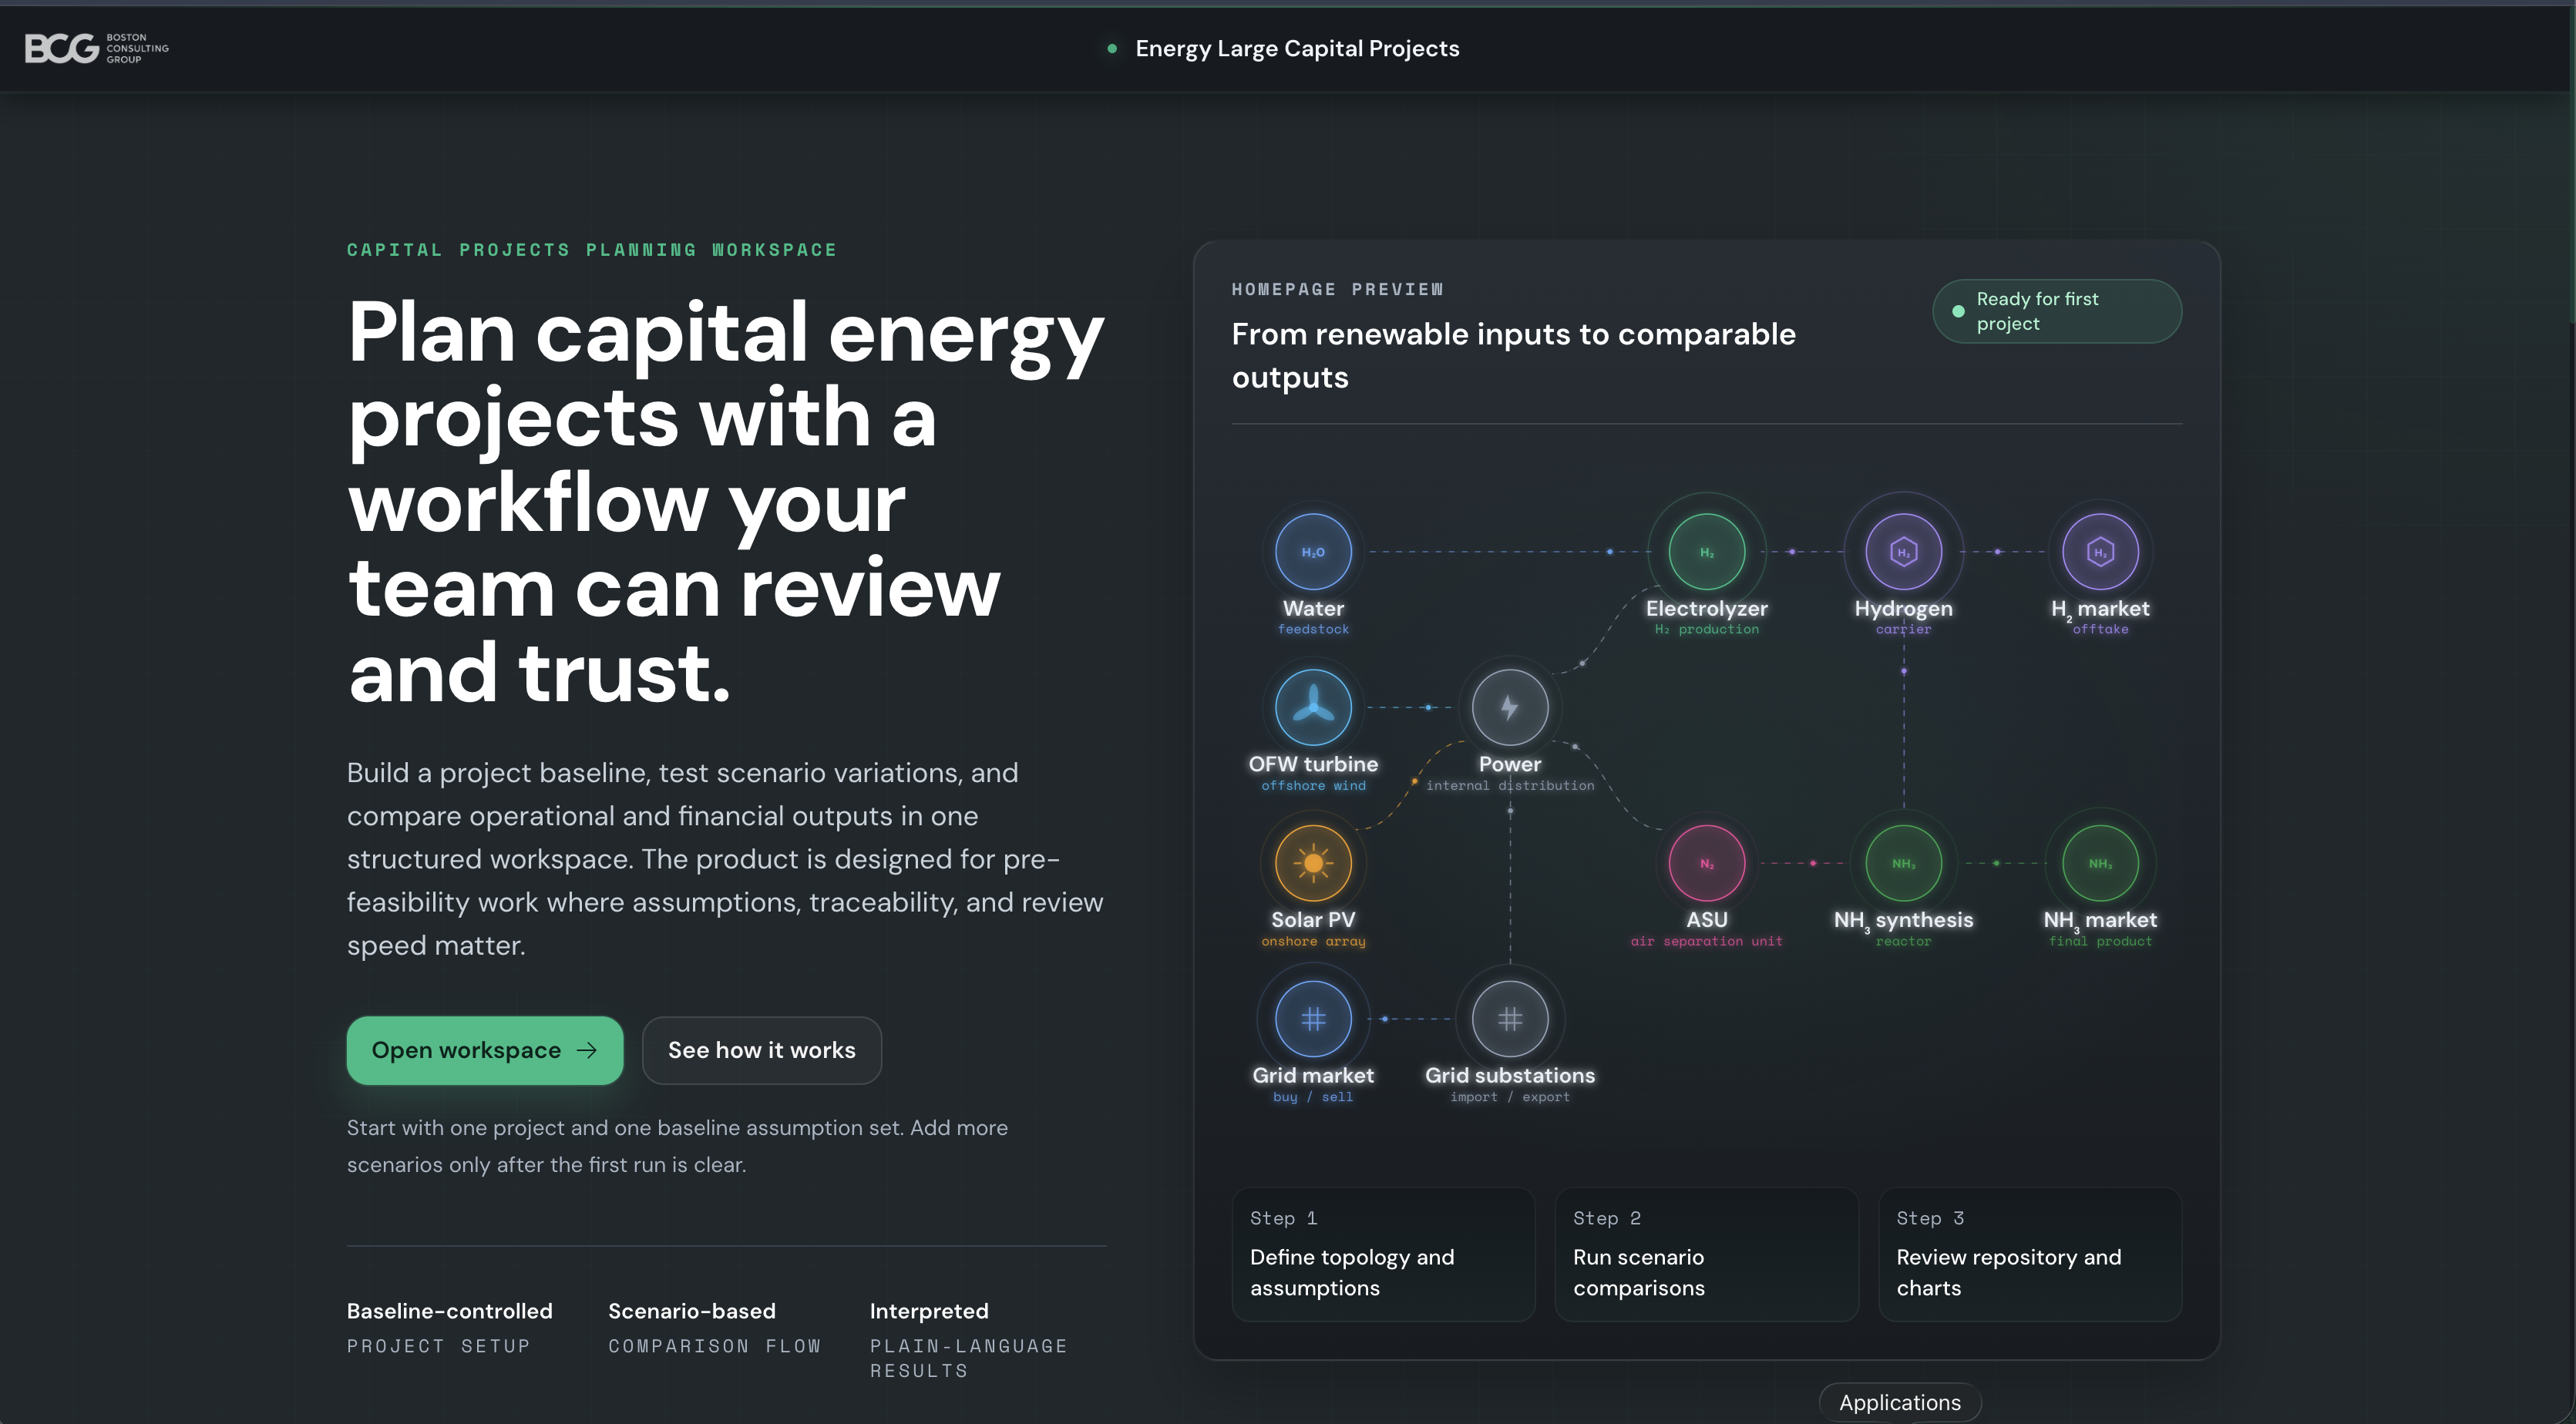
\includegraphics[width=0.95\linewidth]{Figures/chadi_landing.png}
  \caption{Landing page: the optimizer framed as a structured, reviewable workflow.}
  \label{fig:impl-landing}
\end{figure}

\begin{figure}[H]
  \centering
  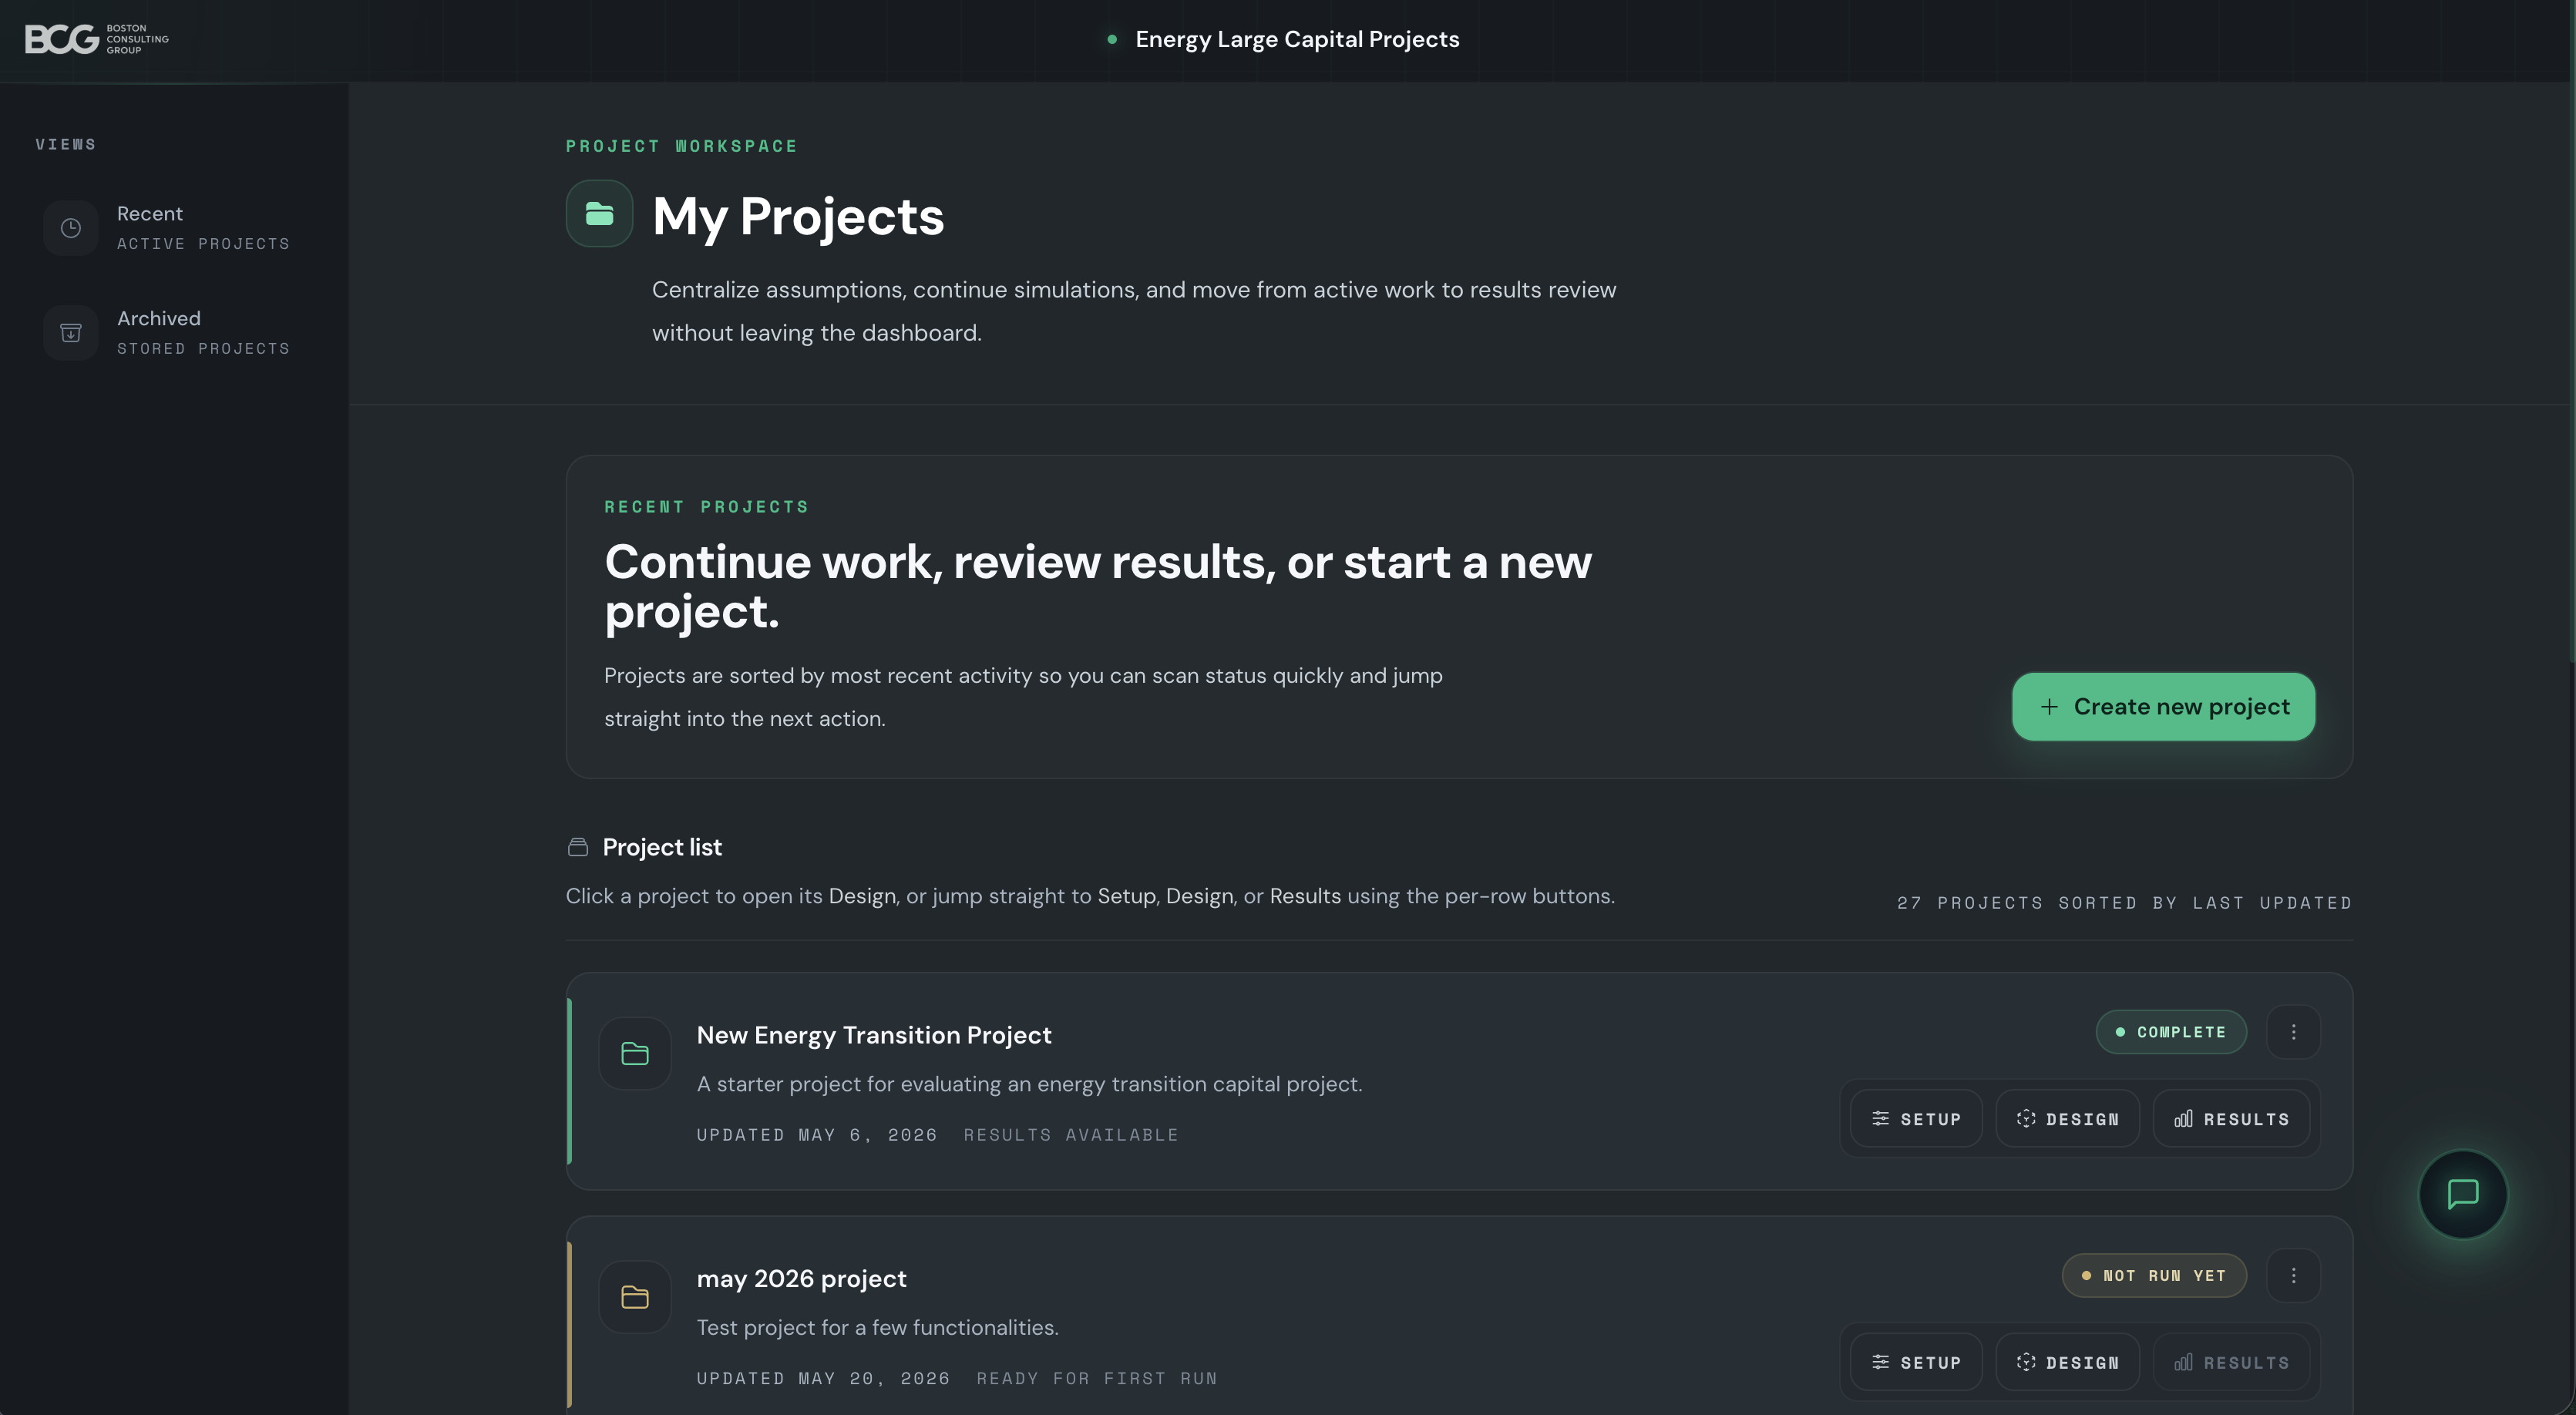
\includegraphics[width=0.95\linewidth]{Figures/chadi_recent_projects.png}
  \caption{Recent projects: continue existing work or start anew from one surface.}
  \label{fig:impl-recent}
\end{figure}

\subsection{Project setup and the deterministic workspace}

The next sequence follows the non-agentic product path: creating a project,
entering assumptions, reviewing and editing the topology, setting parameters and
operating choices, launching simulations, and analyzing deterministic results
(Figures~\ref{fig:impl-data}--\ref{fig:impl-runcharts}). This keeps the
narrative honest: the agentic layer extends a working analytical product, it does
not replace it.

\begin{figure}[H]
  \centering
  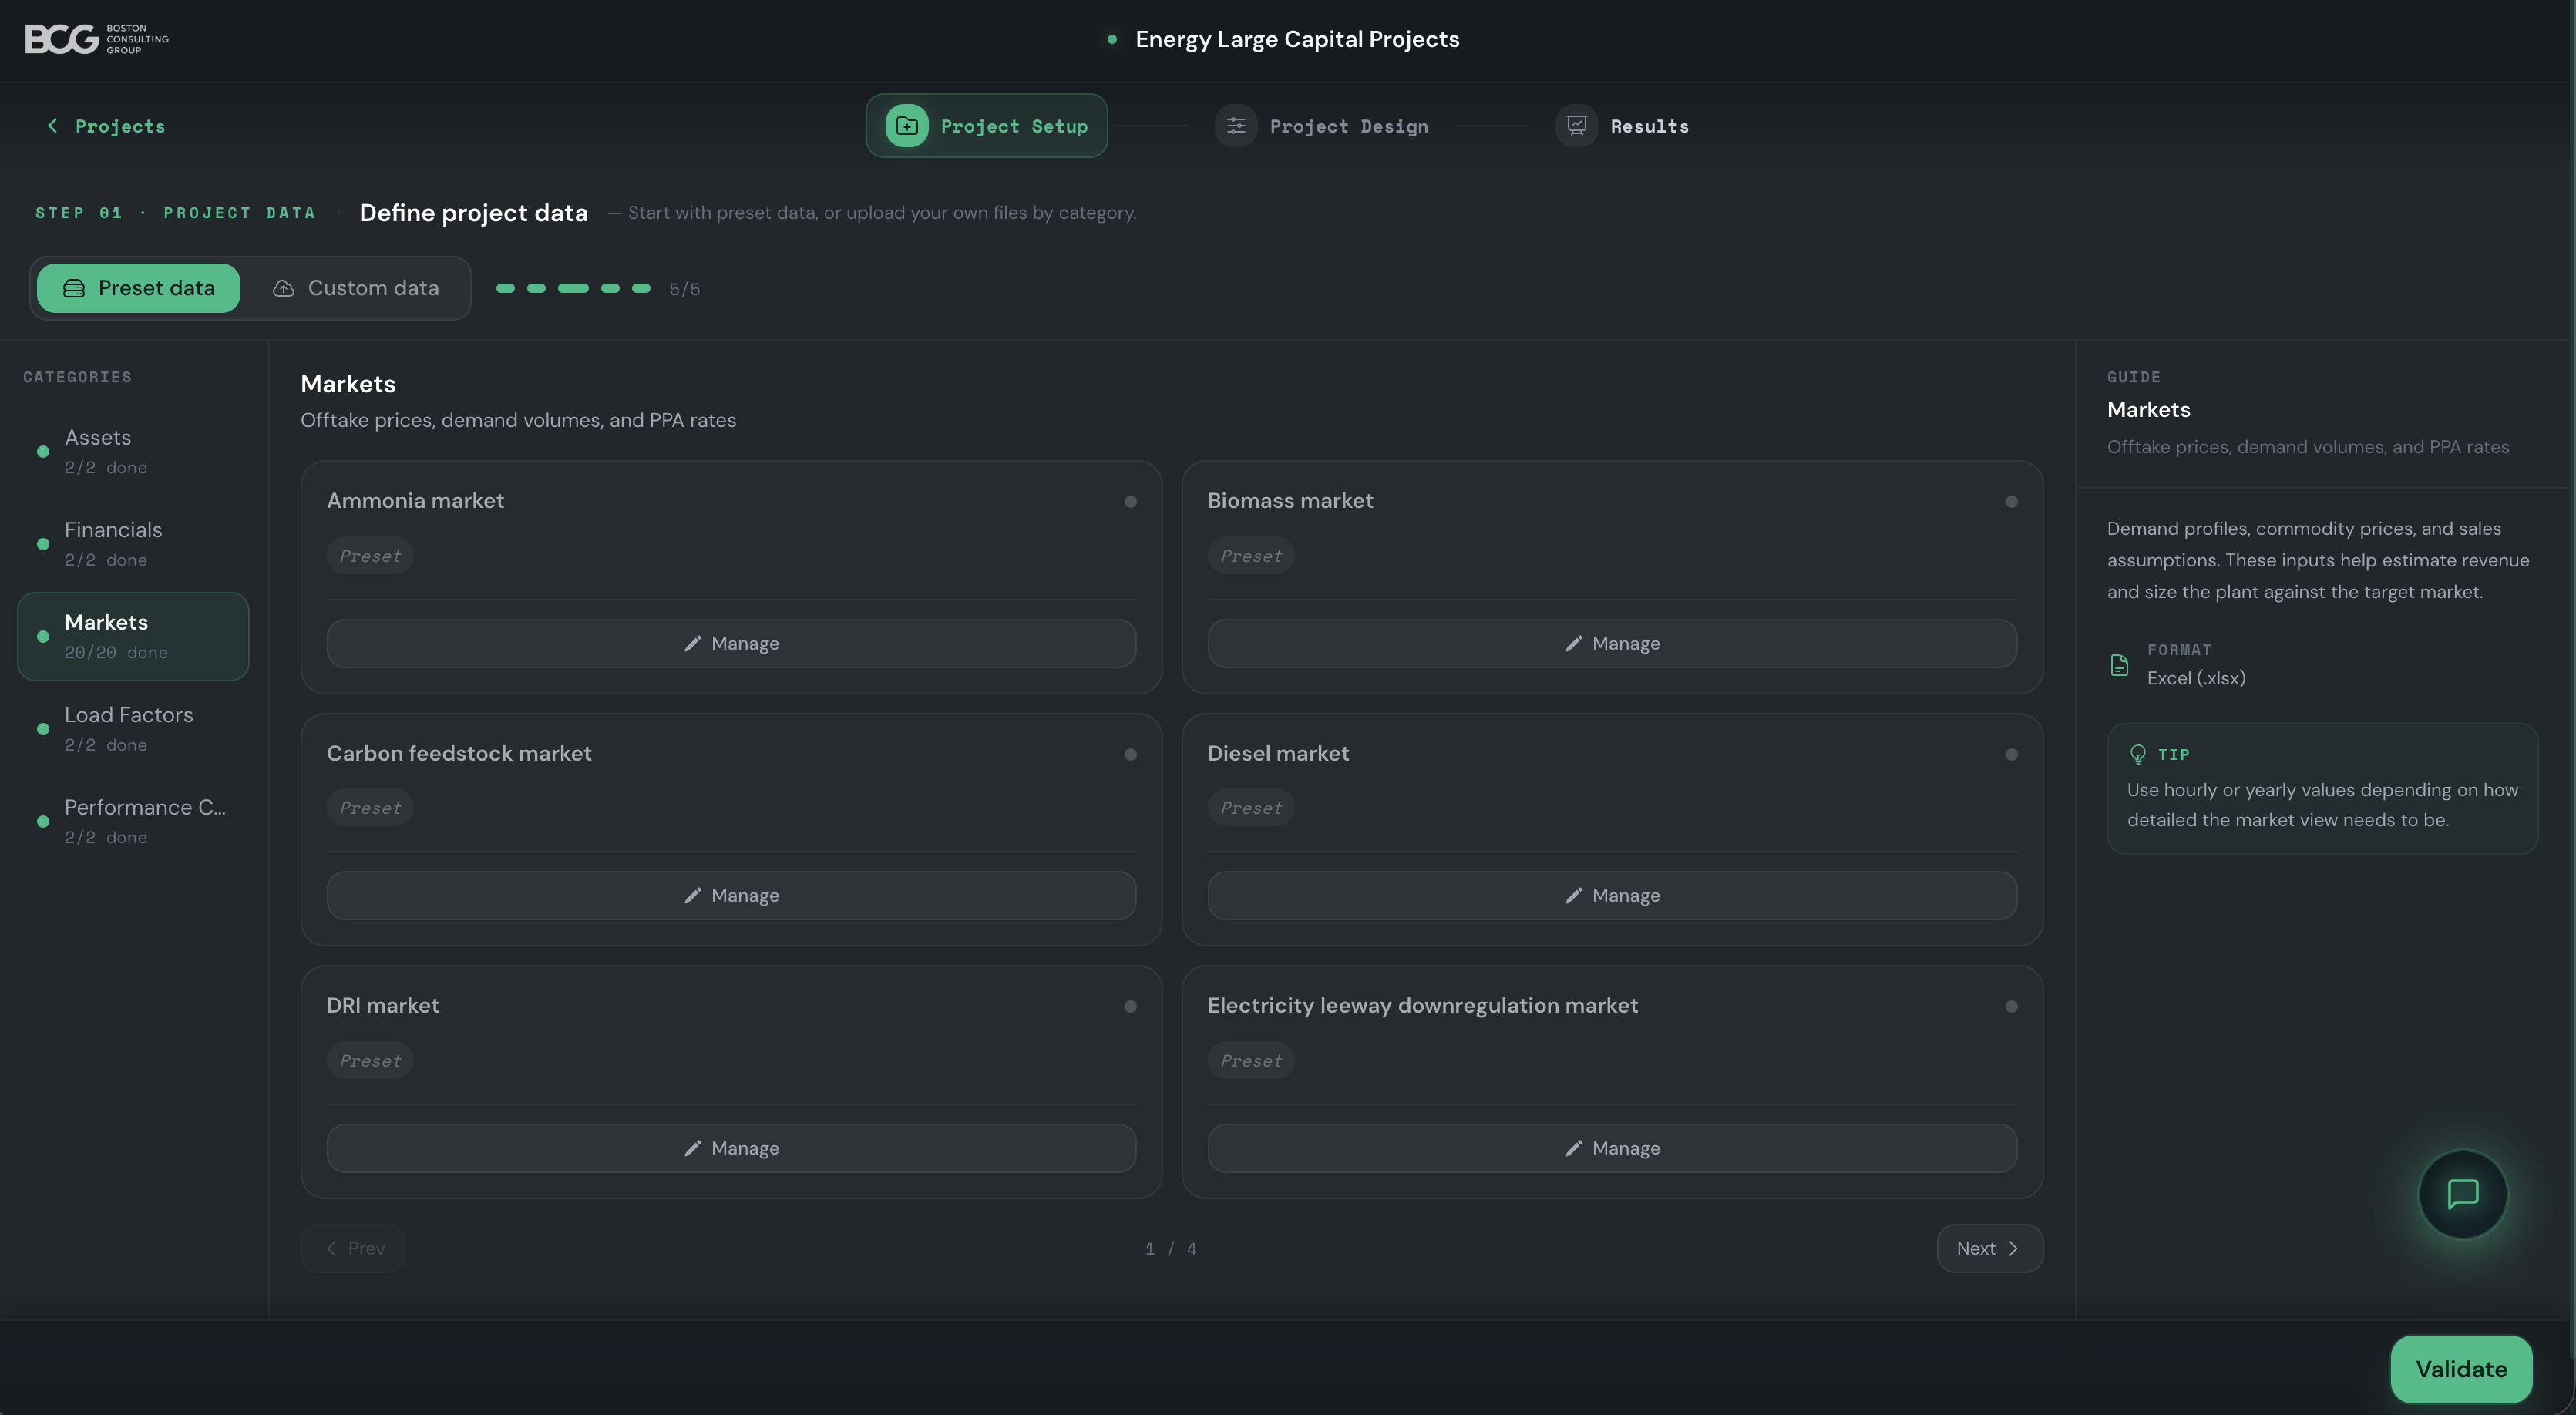
\includegraphics[width=0.95\linewidth]{Figures/chadi_project_data.png}
  \caption{Project data: assets, markets, financing, taxes, and performance inputs.}
  \label{fig:impl-data}
\end{figure}

\begin{figure}[H]
  \centering
  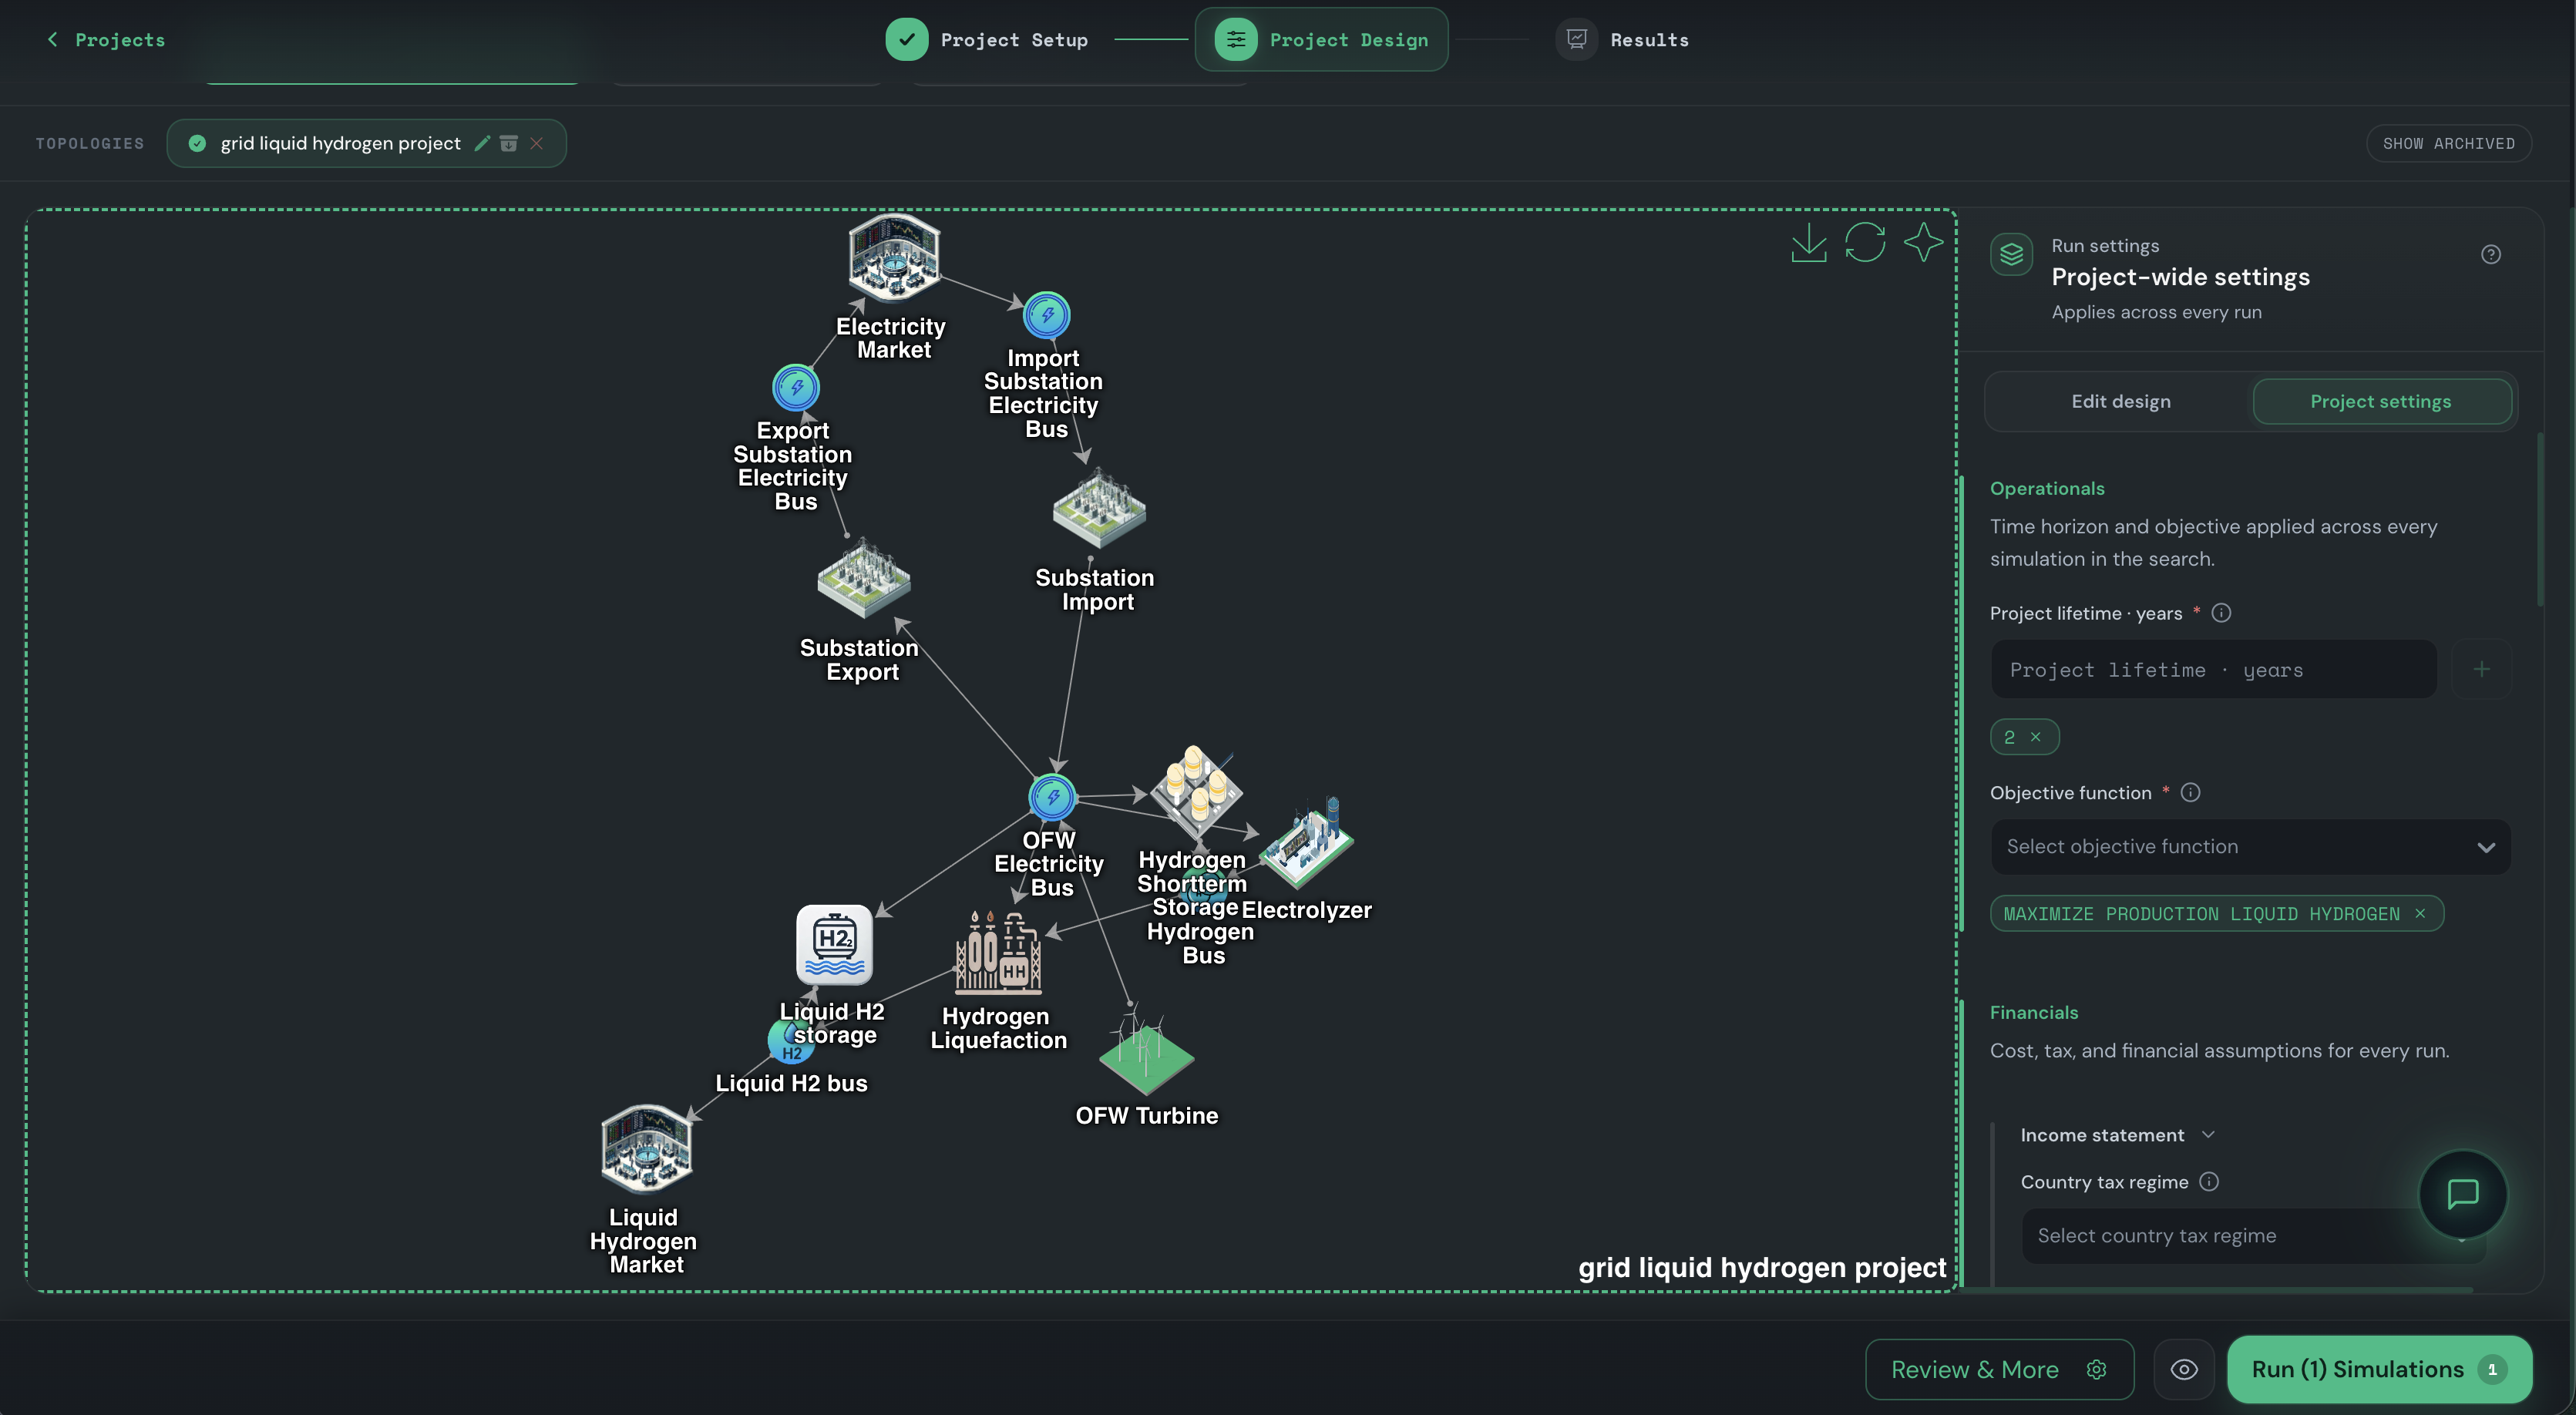
\includegraphics[width=0.95\linewidth]{Figures/chadi_topology_workspace.png}
  \caption{Topology workspace: the project graph, editable and the launch point for simulations.}
  \label{fig:impl-topo}
\end{figure}

\begin{figure}[H]
  \centering
  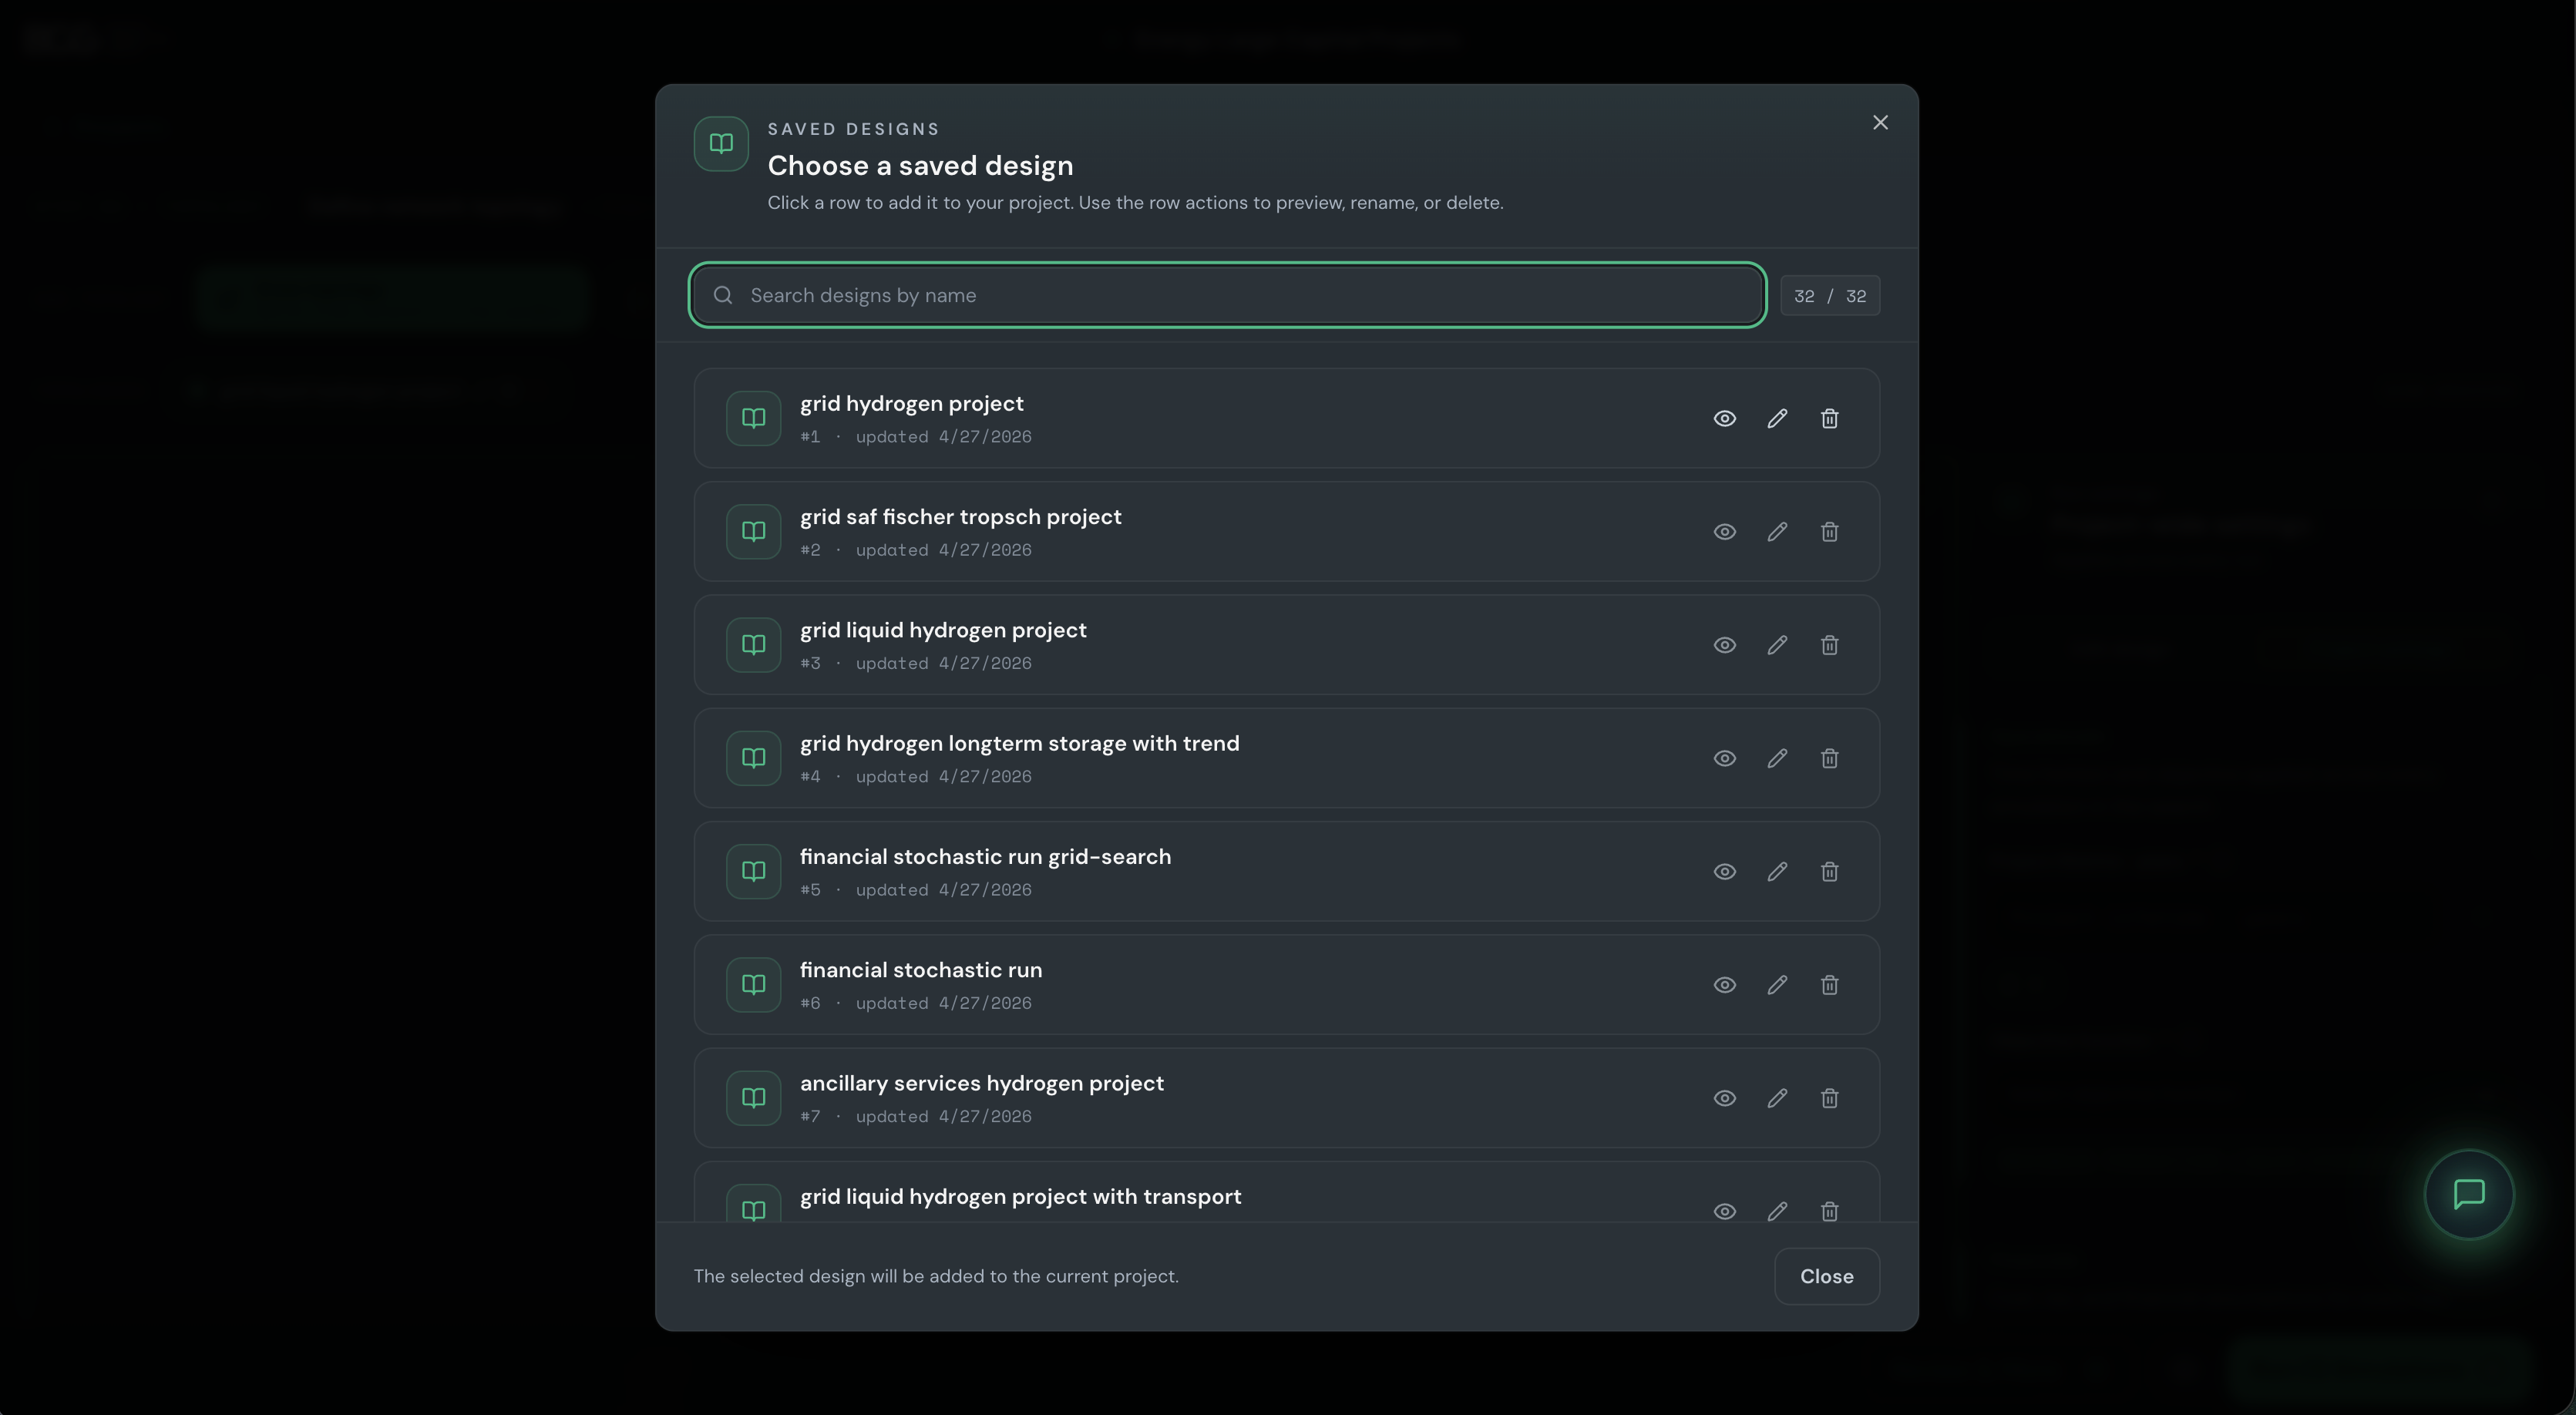
\includegraphics[width=0.95\linewidth]{Figures/chadi_saved_designs.png}
  \caption{Saved designs: reusable topology templates as starting points.}
  \label{fig:impl-saved}
\end{figure}

\begin{figure}[H]
  \centering
  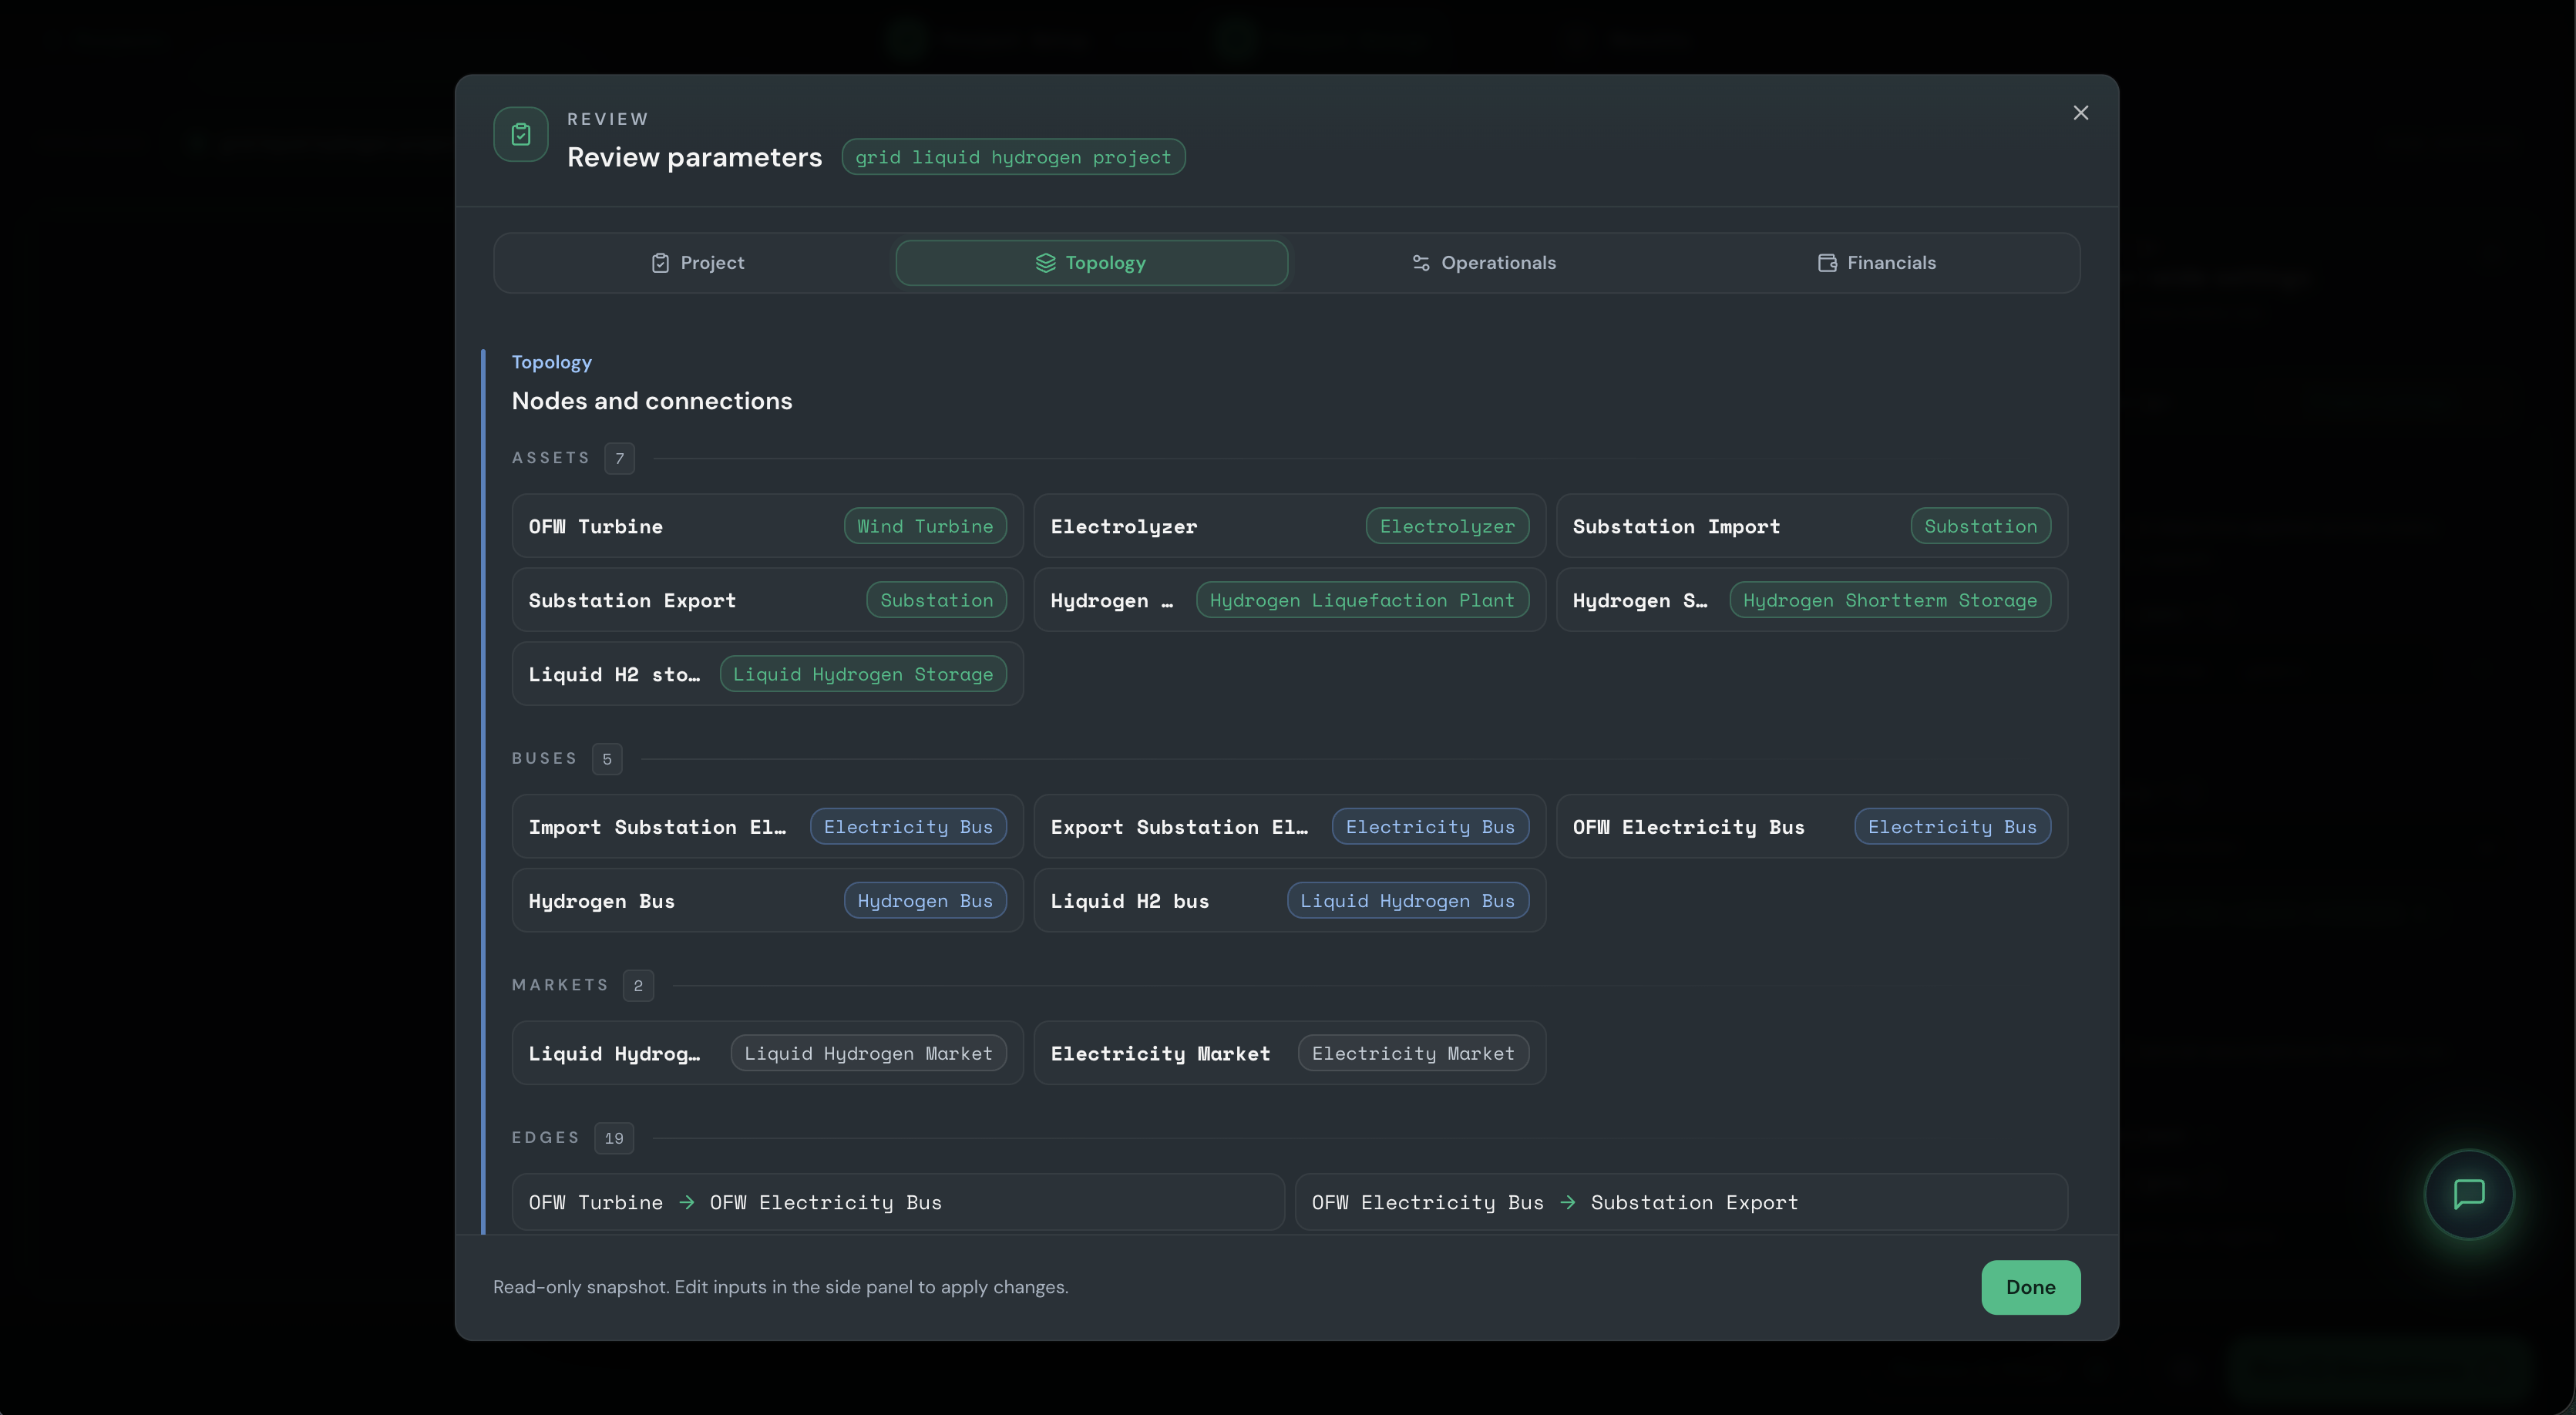
\includegraphics[width=0.95\linewidth]{Figures/chadi_topology_params.png}
  \caption{Topology parameters: component-level assumptions the engine consumes.}
  \label{fig:impl-topoparams}
\end{figure}

\begin{figure}[H]
  \centering
  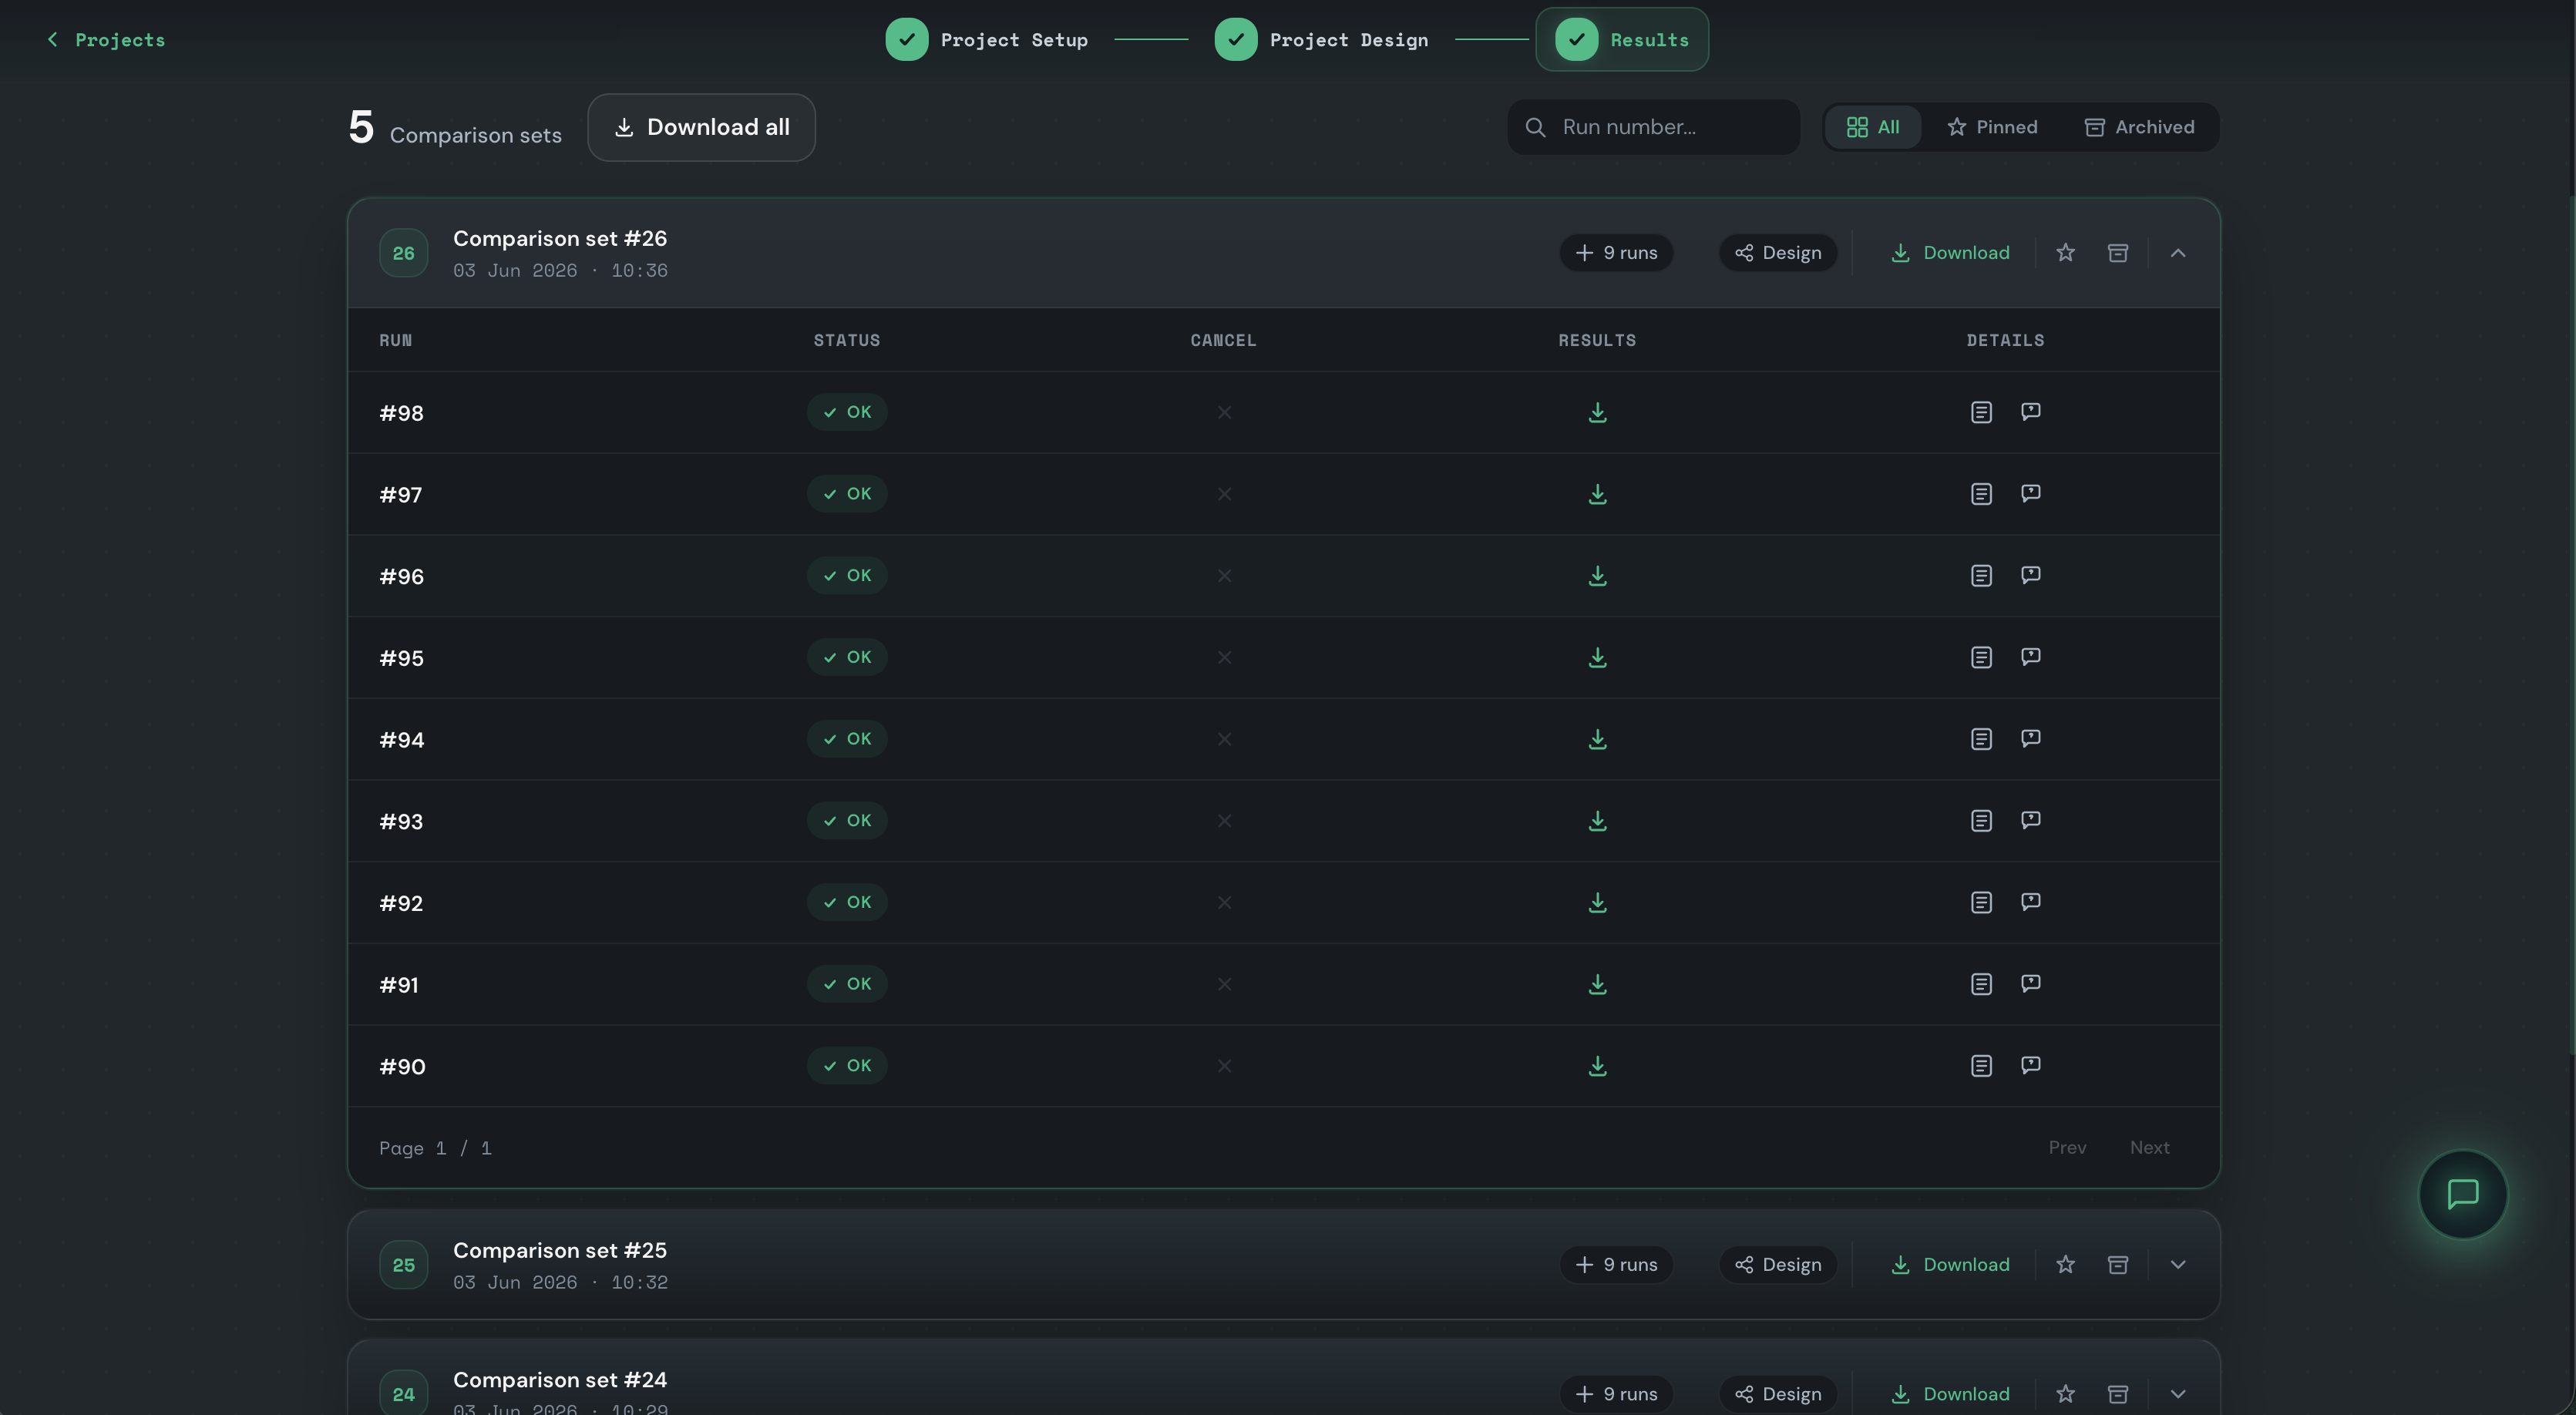
\includegraphics[width=0.95\linewidth]{Figures/chadi_comparison_table.png}
  \caption{Comparison table: deterministic outputs across runs in a dense review format.}
  \label{fig:impl-comptable}
\end{figure}

\begin{figure}[H]
  \centering
  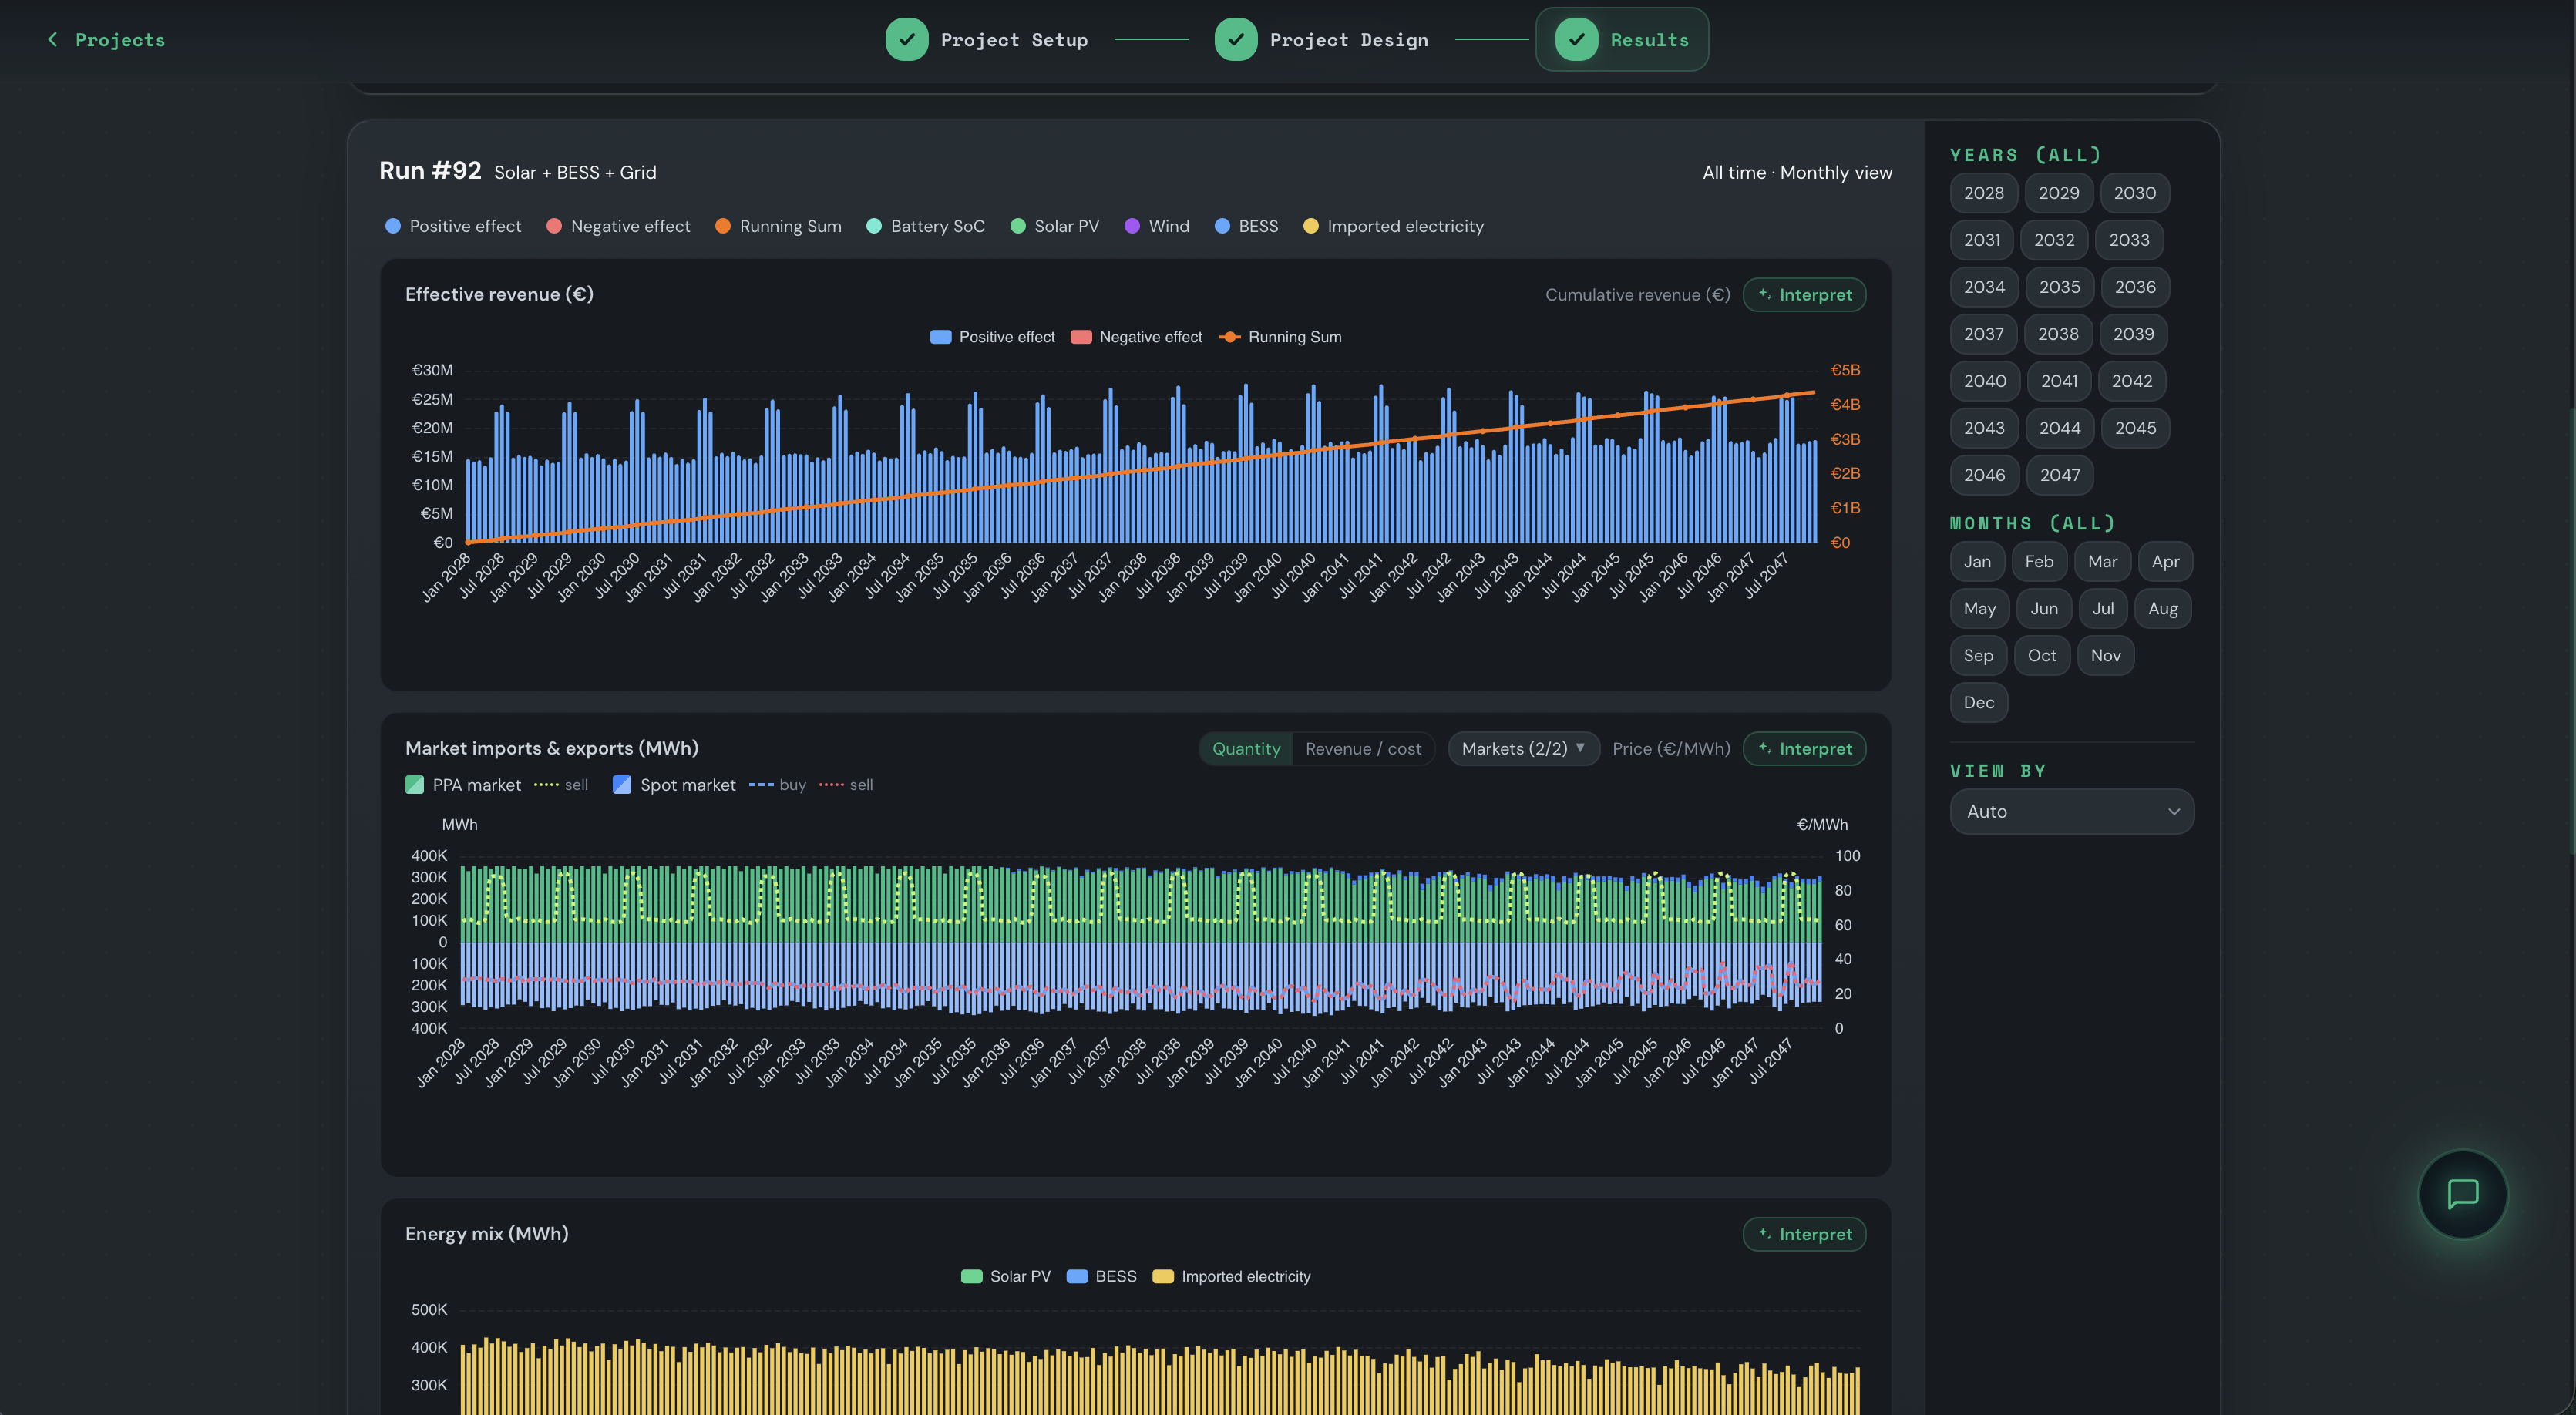
\includegraphics[width=0.95\linewidth]{Figures/chadi_run_charts.png}
  \caption{Run charts: effective revenue and market imports and exports with time filters.}
  \label{fig:impl-runcharts}
\end{figure}

\subsection{Agentic project creation}

Once the restored application path is visible, the sequence shifts to the agentic
layer. The first conversation demonstrates discovery, intent capture, and
approval-gated creation
(Figures~\ref{fig:impl-agentpanel}--\ref{fig:impl-postapproval}). The
implementation point is control: the agent helps the user move faster, but
important state changes still pass through explicit proposal and approval steps.

\begin{figure}[H]
  \centering
  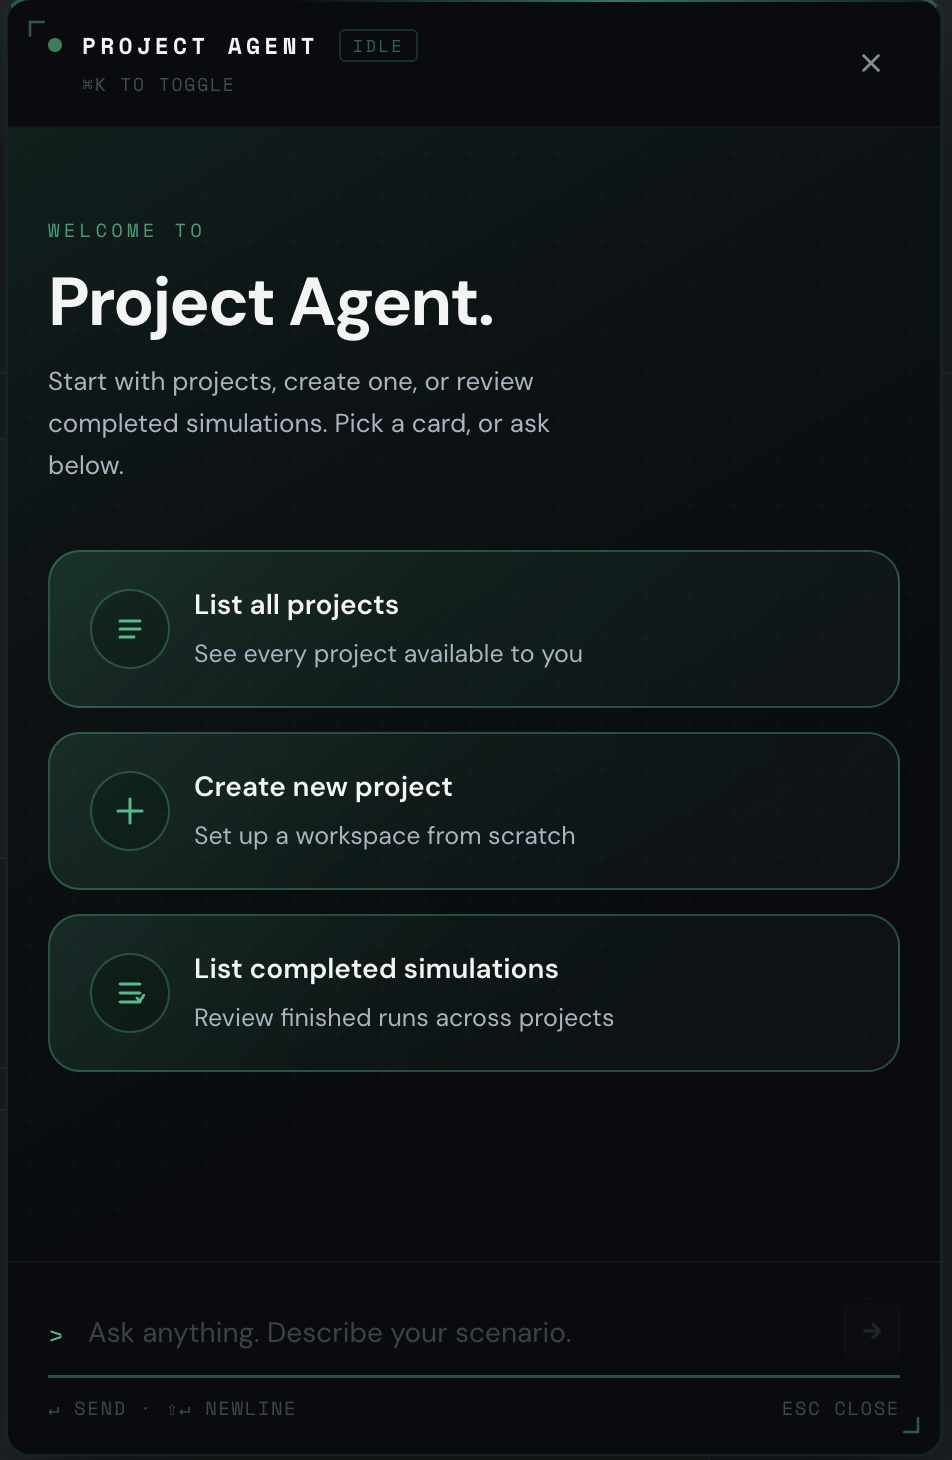
\includegraphics[width=0.48\linewidth]{Figures/chadi_agent_panel.png}
  \caption{Agent command panel: guided entry points and a free-form prompt.}
  \label{fig:impl-agentpanel}
\end{figure}

\begin{figure}[H]
  \centering
  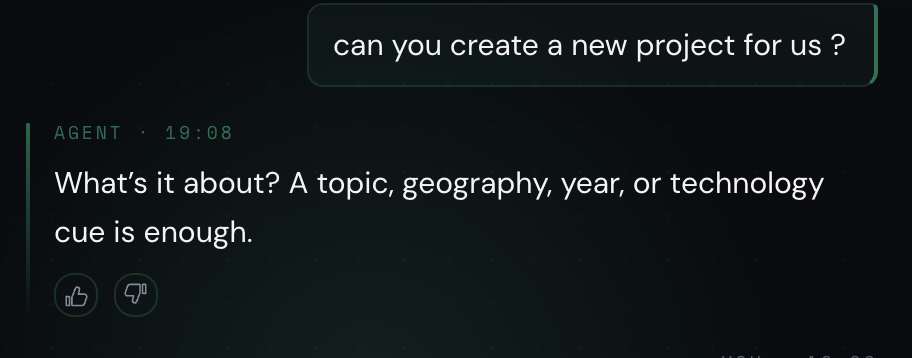
\includegraphics[width=0.62\linewidth]{Figures/chadi_intent_capture.png}
  \caption{Intent capture: the agent asks for a topic, geography, year, or technology cue.}
  \label{fig:impl-intent}
\end{figure}

\begin{figure}[H]
  \centering
  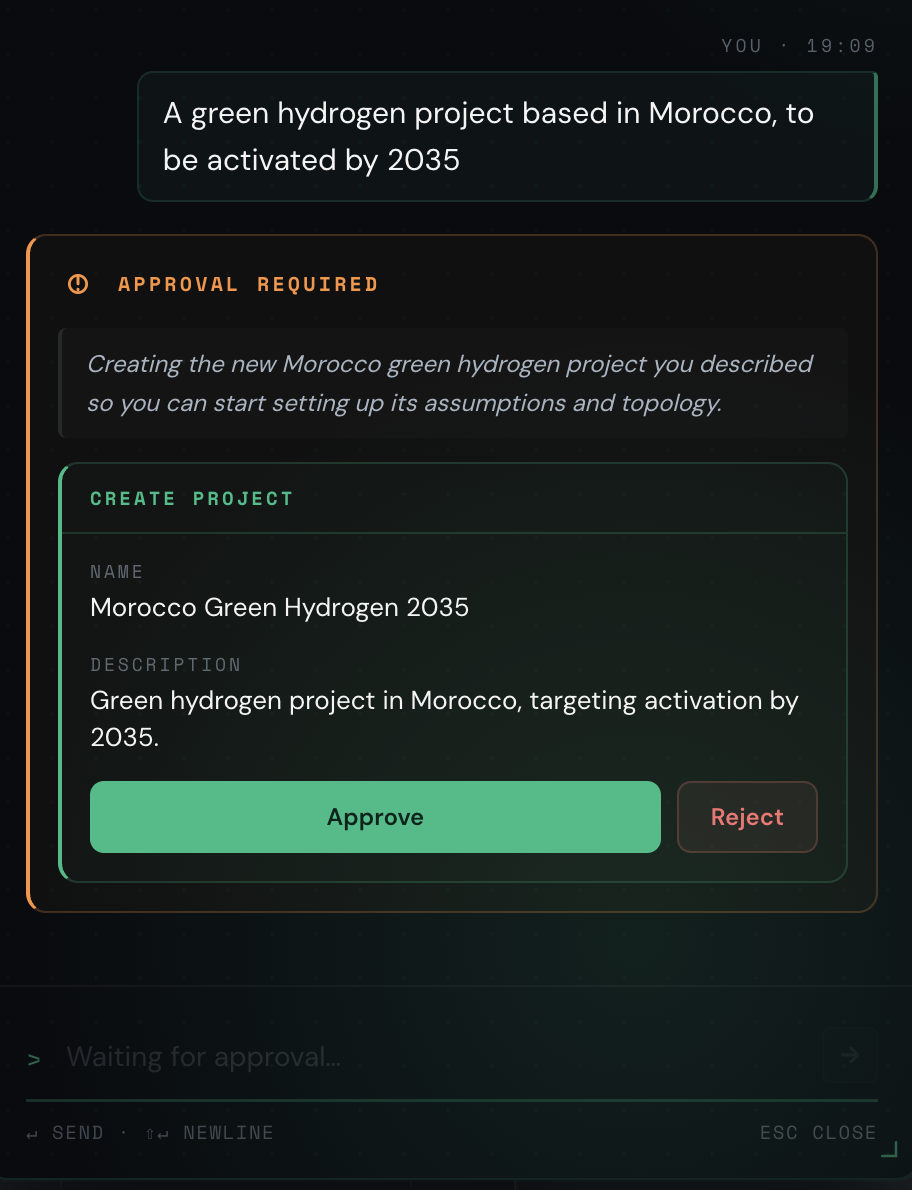
\includegraphics[width=0.5\linewidth]{Figures/chadi_approval_card.png}
  \caption{Approval card: a proposed project awaits approval, the first governed write.}
  \label{fig:impl-approval}
\end{figure}

\begin{figure}[H]
  \centering
  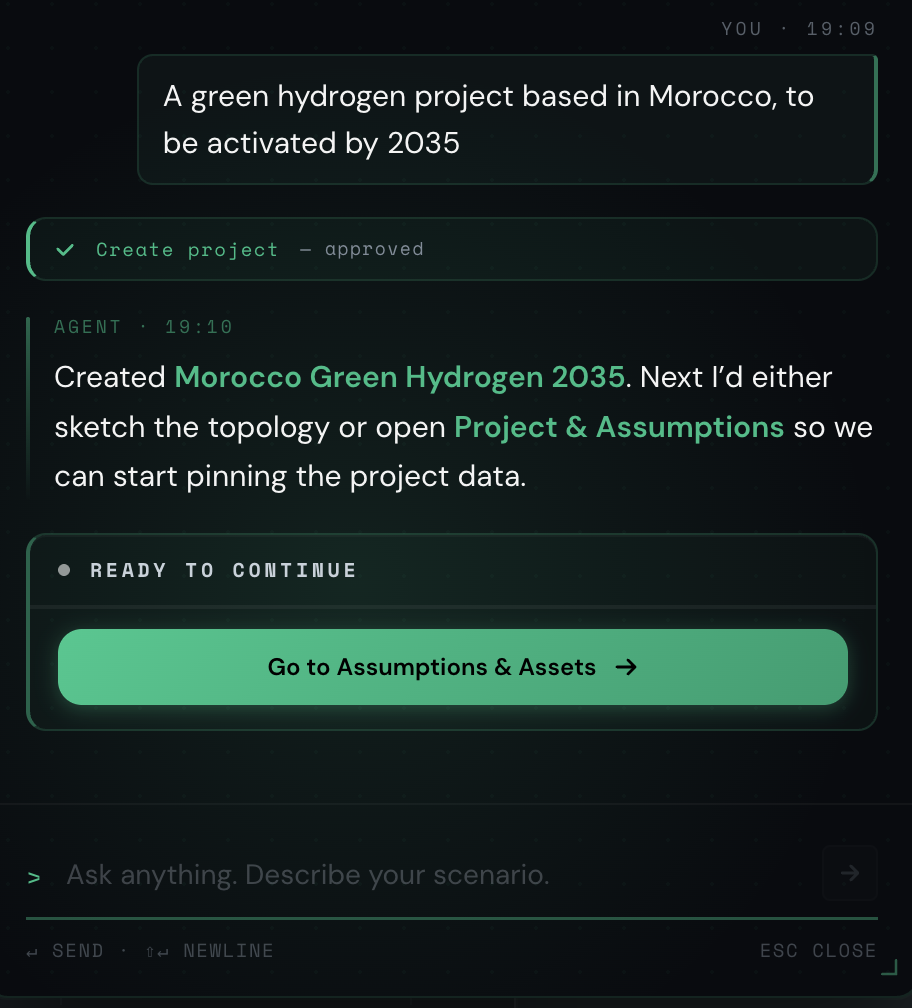
\includegraphics[width=0.55\linewidth]{Figures/chadi_post_approval.png}
  \caption{Post-approval: an approved proposal becomes a concrete product transition.}
  \label{fig:impl-postapproval}
\end{figure}

\subsection{File and assumption ingestion}

Uploaded assumptions can change simulation results directly, so ingestion is a
governed workflow that combines conversational guidance with explicit file review:
the assistant reads project state and reasons about differences, while the
application surfaces previews, matches, conflicts, and review gates before any data
is accepted (Figures~\ref{fig:impl-context}--\ref{fig:impl-review}).

\begin{figure}[H]
  \centering
  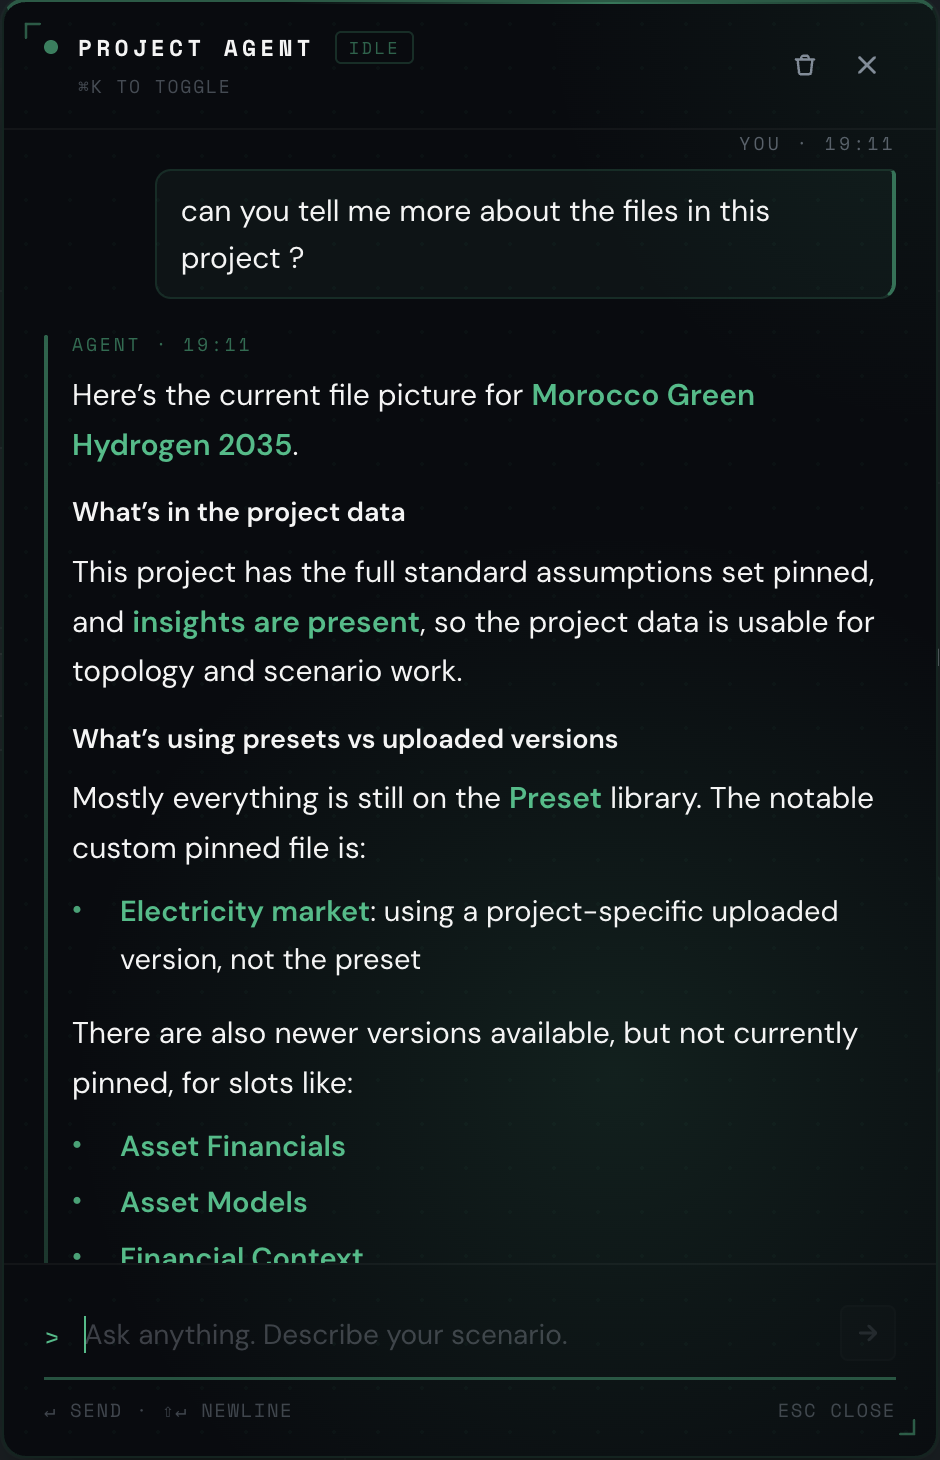
\includegraphics[width=0.48\linewidth]{Figures/chadi_context_retrieval.png}
  \caption{Context retrieval: which assumption files and versions are attached.}
  \label{fig:impl-context}
\end{figure}

\begin{figure}[H]
  \centering
  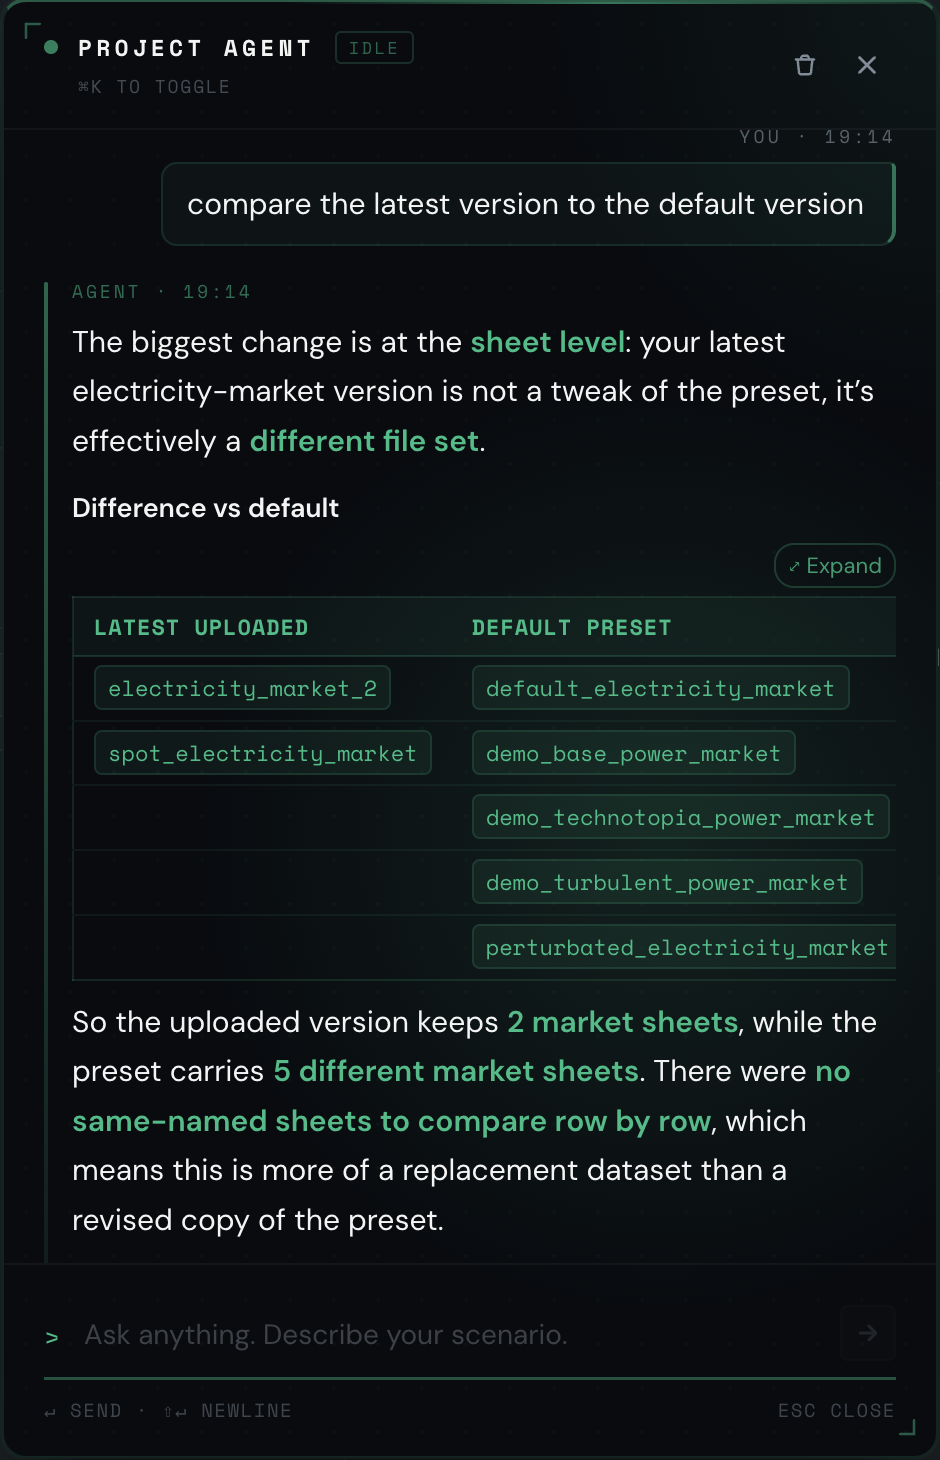
\includegraphics[width=0.48\linewidth]{Figures/chadi_file_comparison.png}
  \caption{File comparison: an uploaded sheet compared with the preset, sheet by sheet.}
  \label{fig:impl-filecomparison}
\end{figure}

\begin{figure}[H]
  \centering
  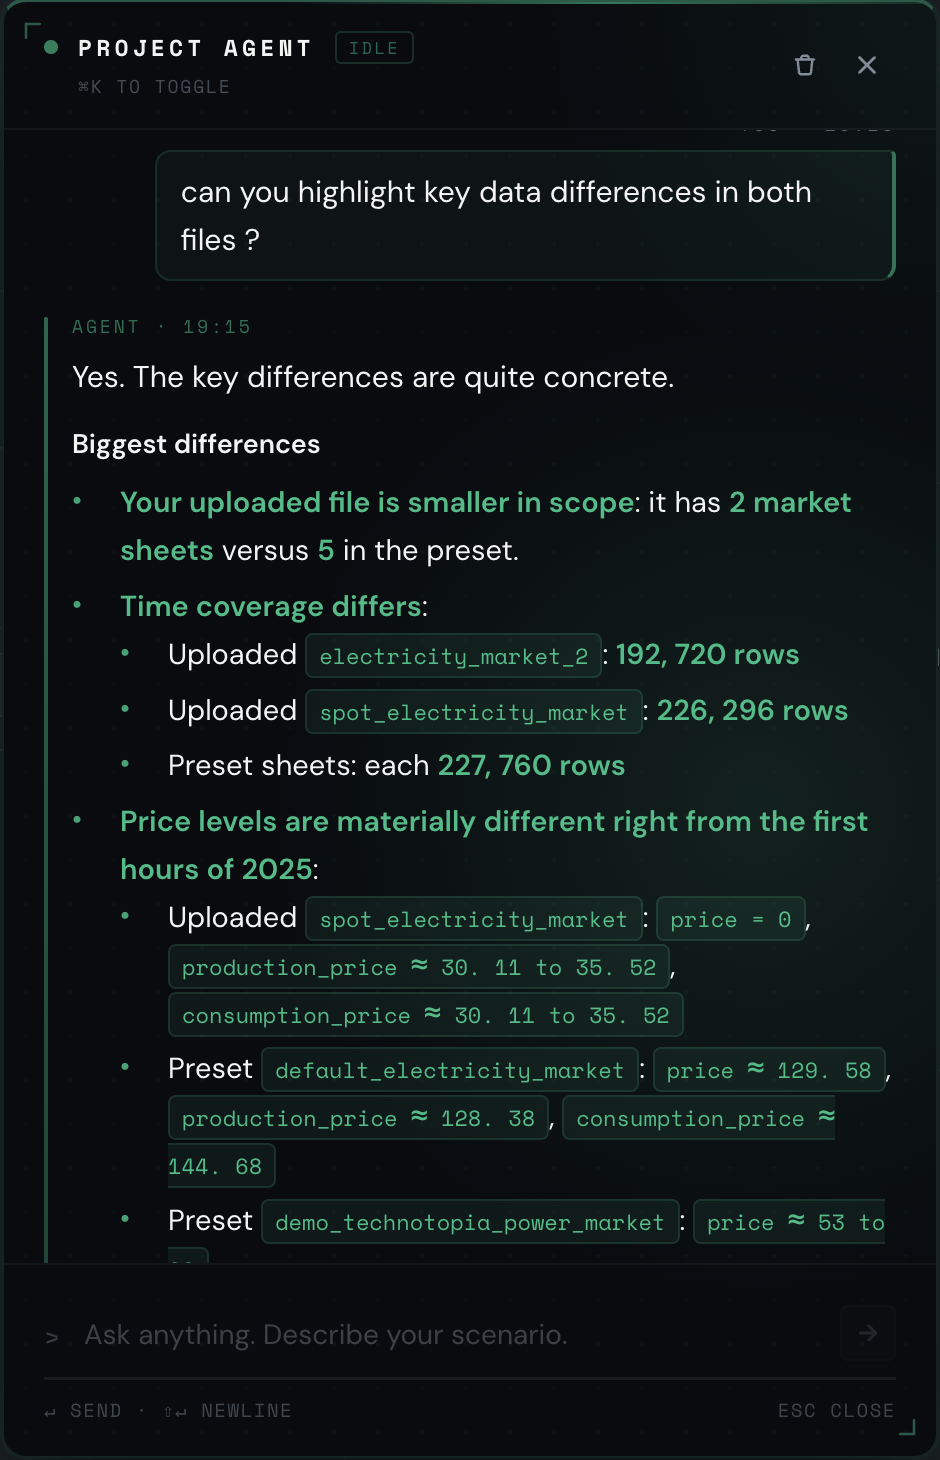
\includegraphics[width=0.48\linewidth]{Figures/chadi_data_differences.png}
  \caption{Data differences: scope, time coverage, and price-level differences made explicit.}
  \label{fig:impl-datadiff}
\end{figure}

\begin{figure}[H]
  \centering
  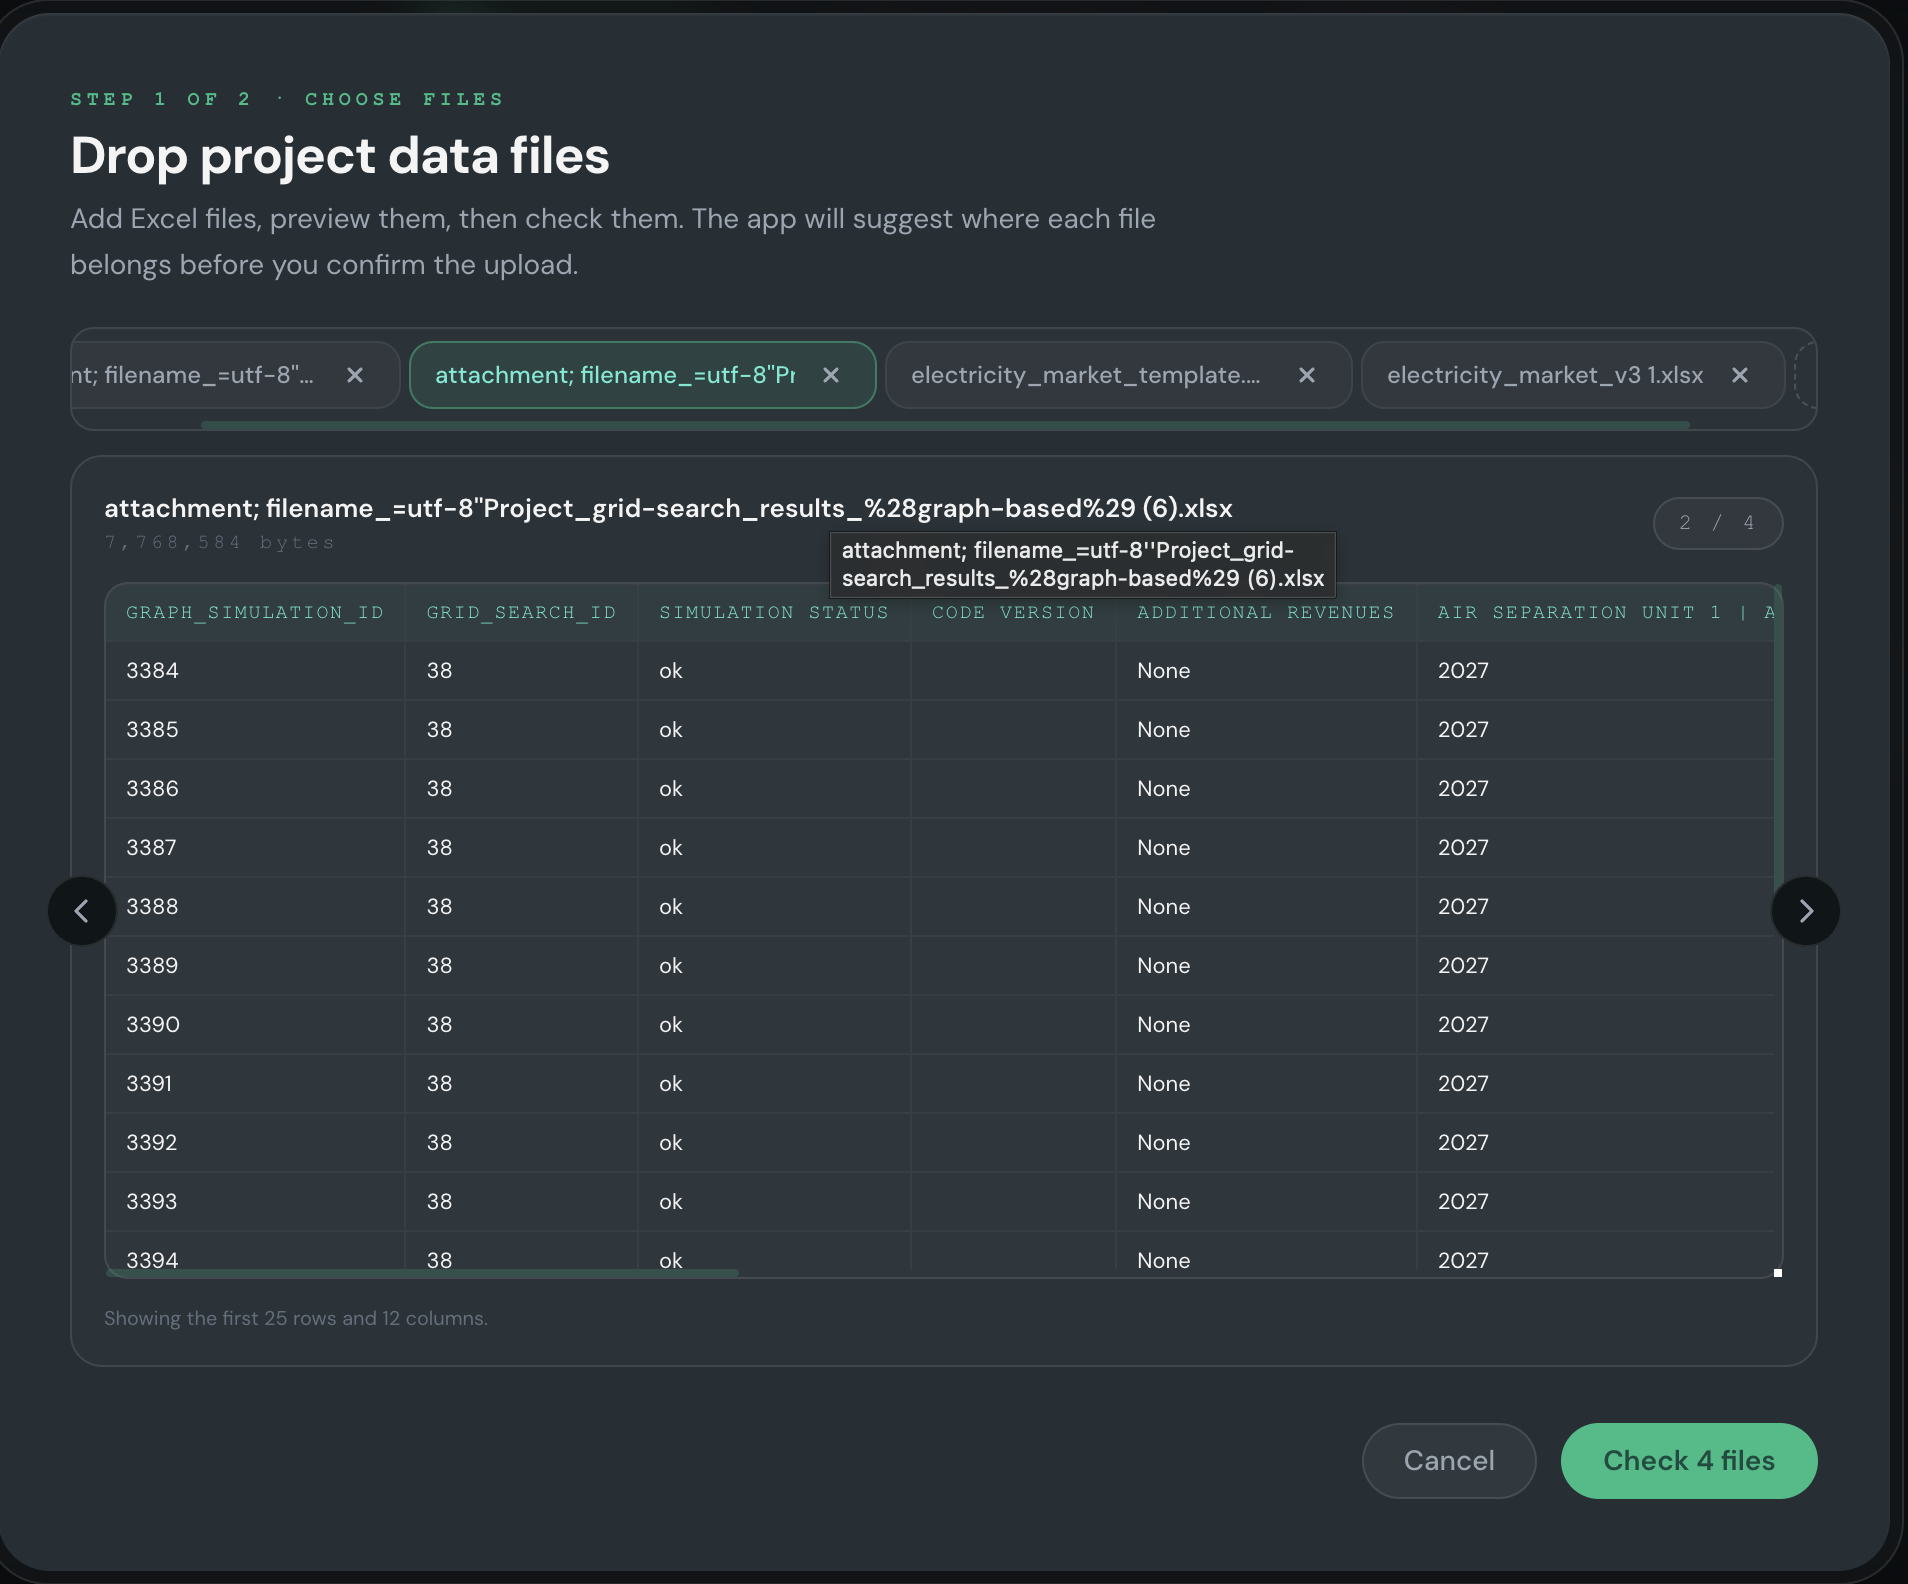
\includegraphics[width=0.72\linewidth]{Figures/chadi_file_preview.png}
  \caption{File preview: workbook and sheet selection with a parsed-row preview.}
  \label{fig:impl-filepreview}
\end{figure}

\begin{figure}[H]
  \centering
  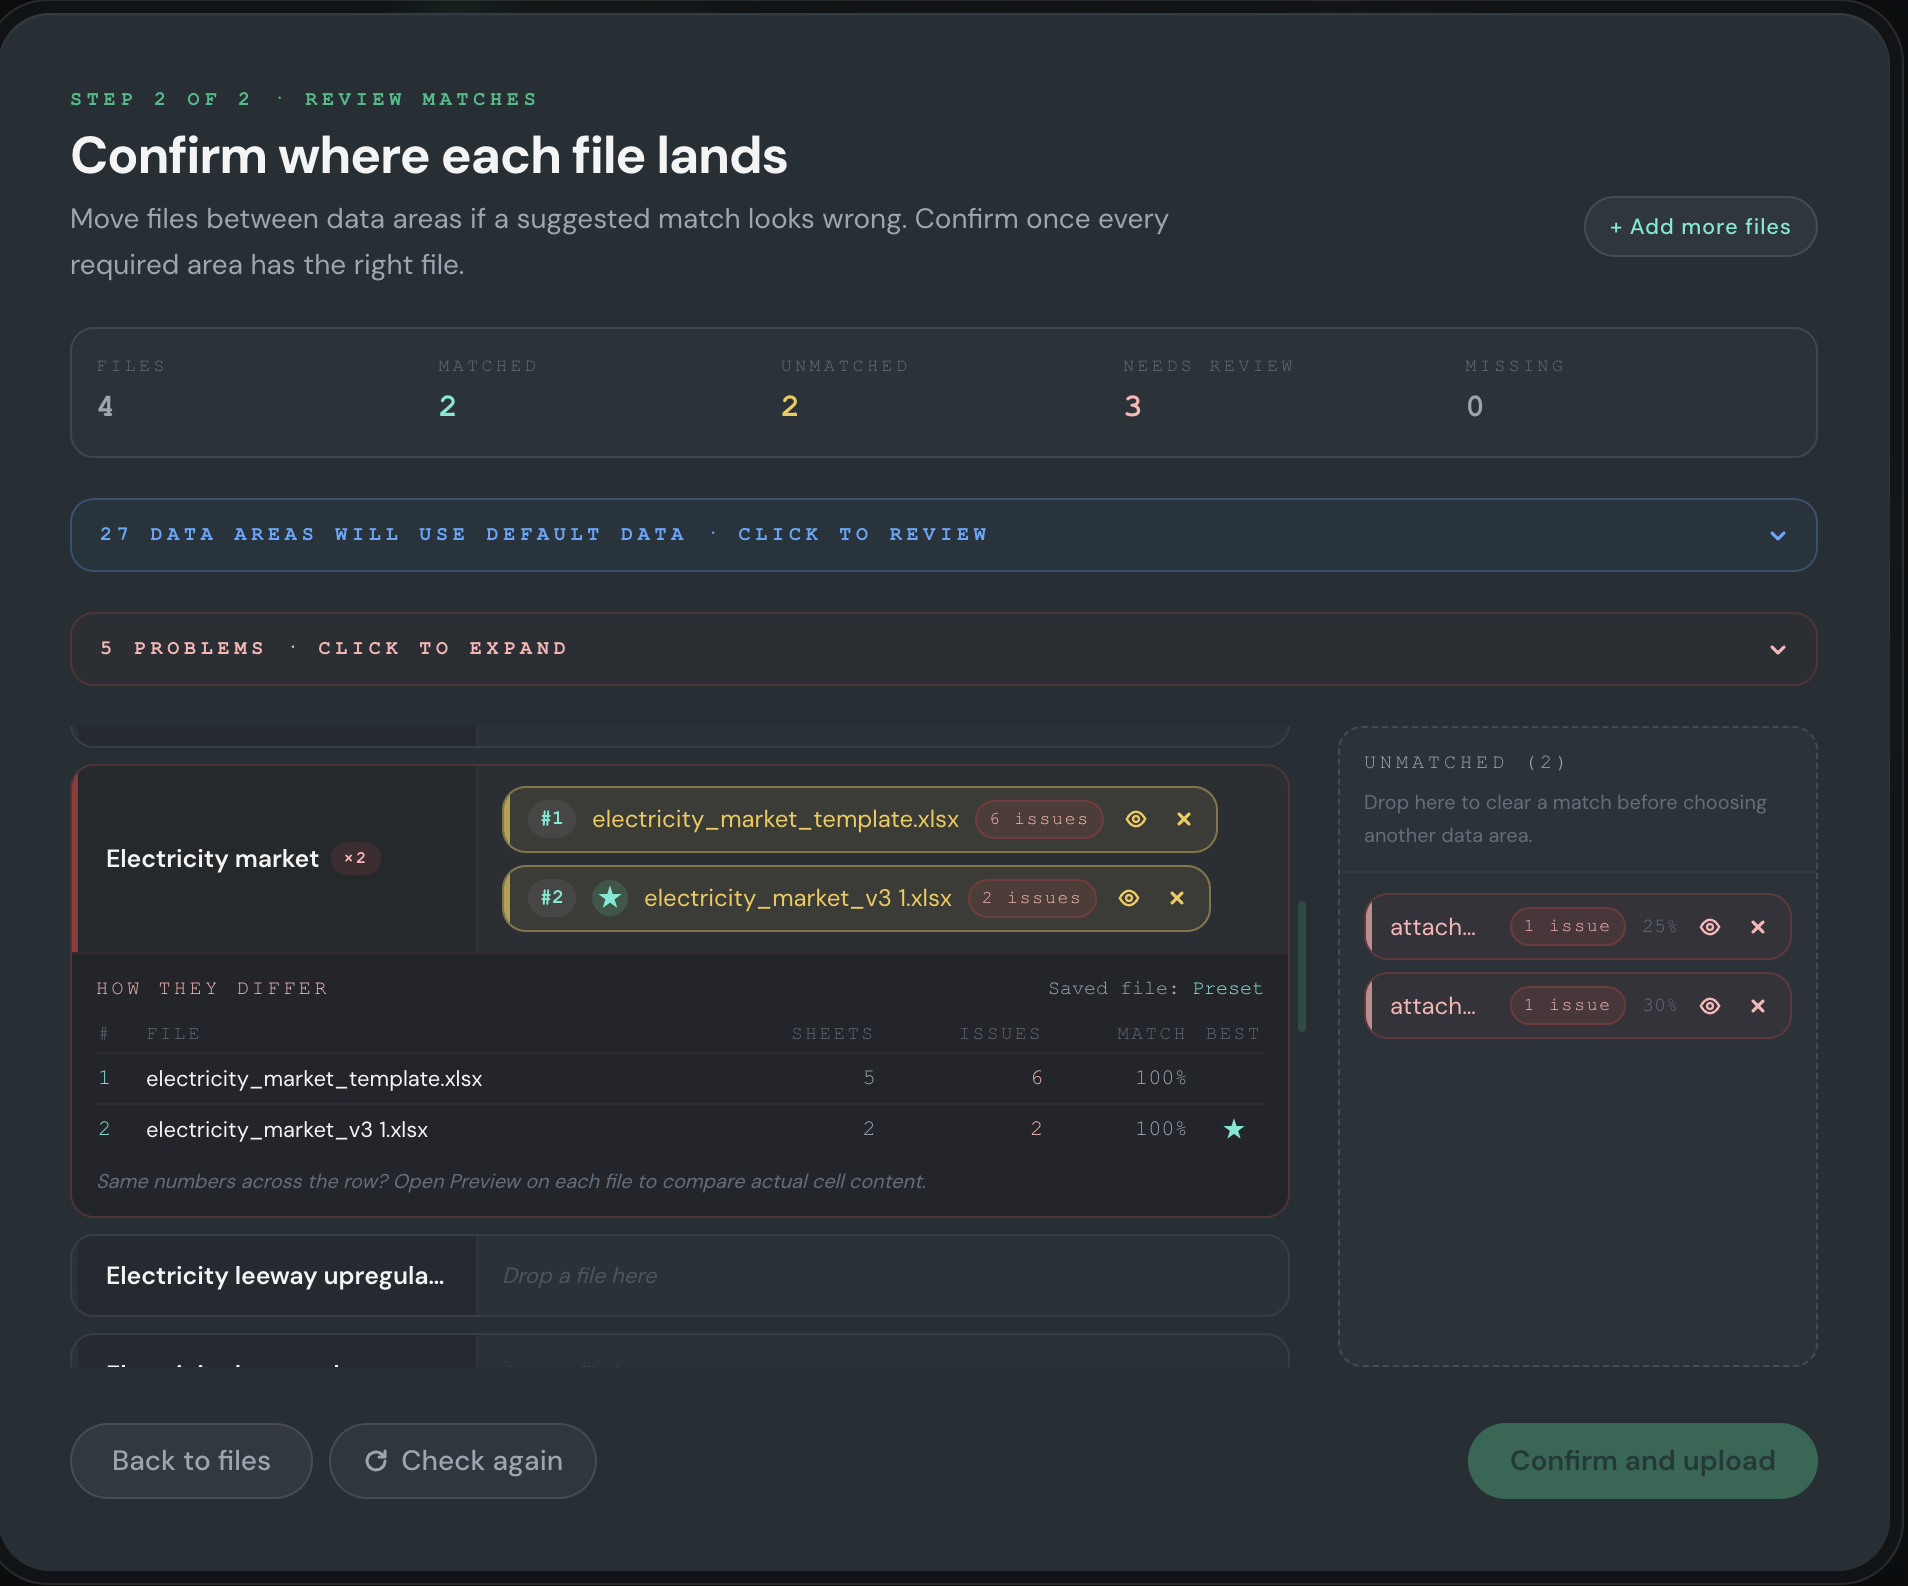
\includegraphics[width=0.72\linewidth]{Figures/chadi_match_confirmation.png}
  \caption{Match confirmation: matched, unmatched, review-needed, and missing areas, gated.}
  \label{fig:impl-match}
\end{figure}

\begin{figure}[H]
  \centering
  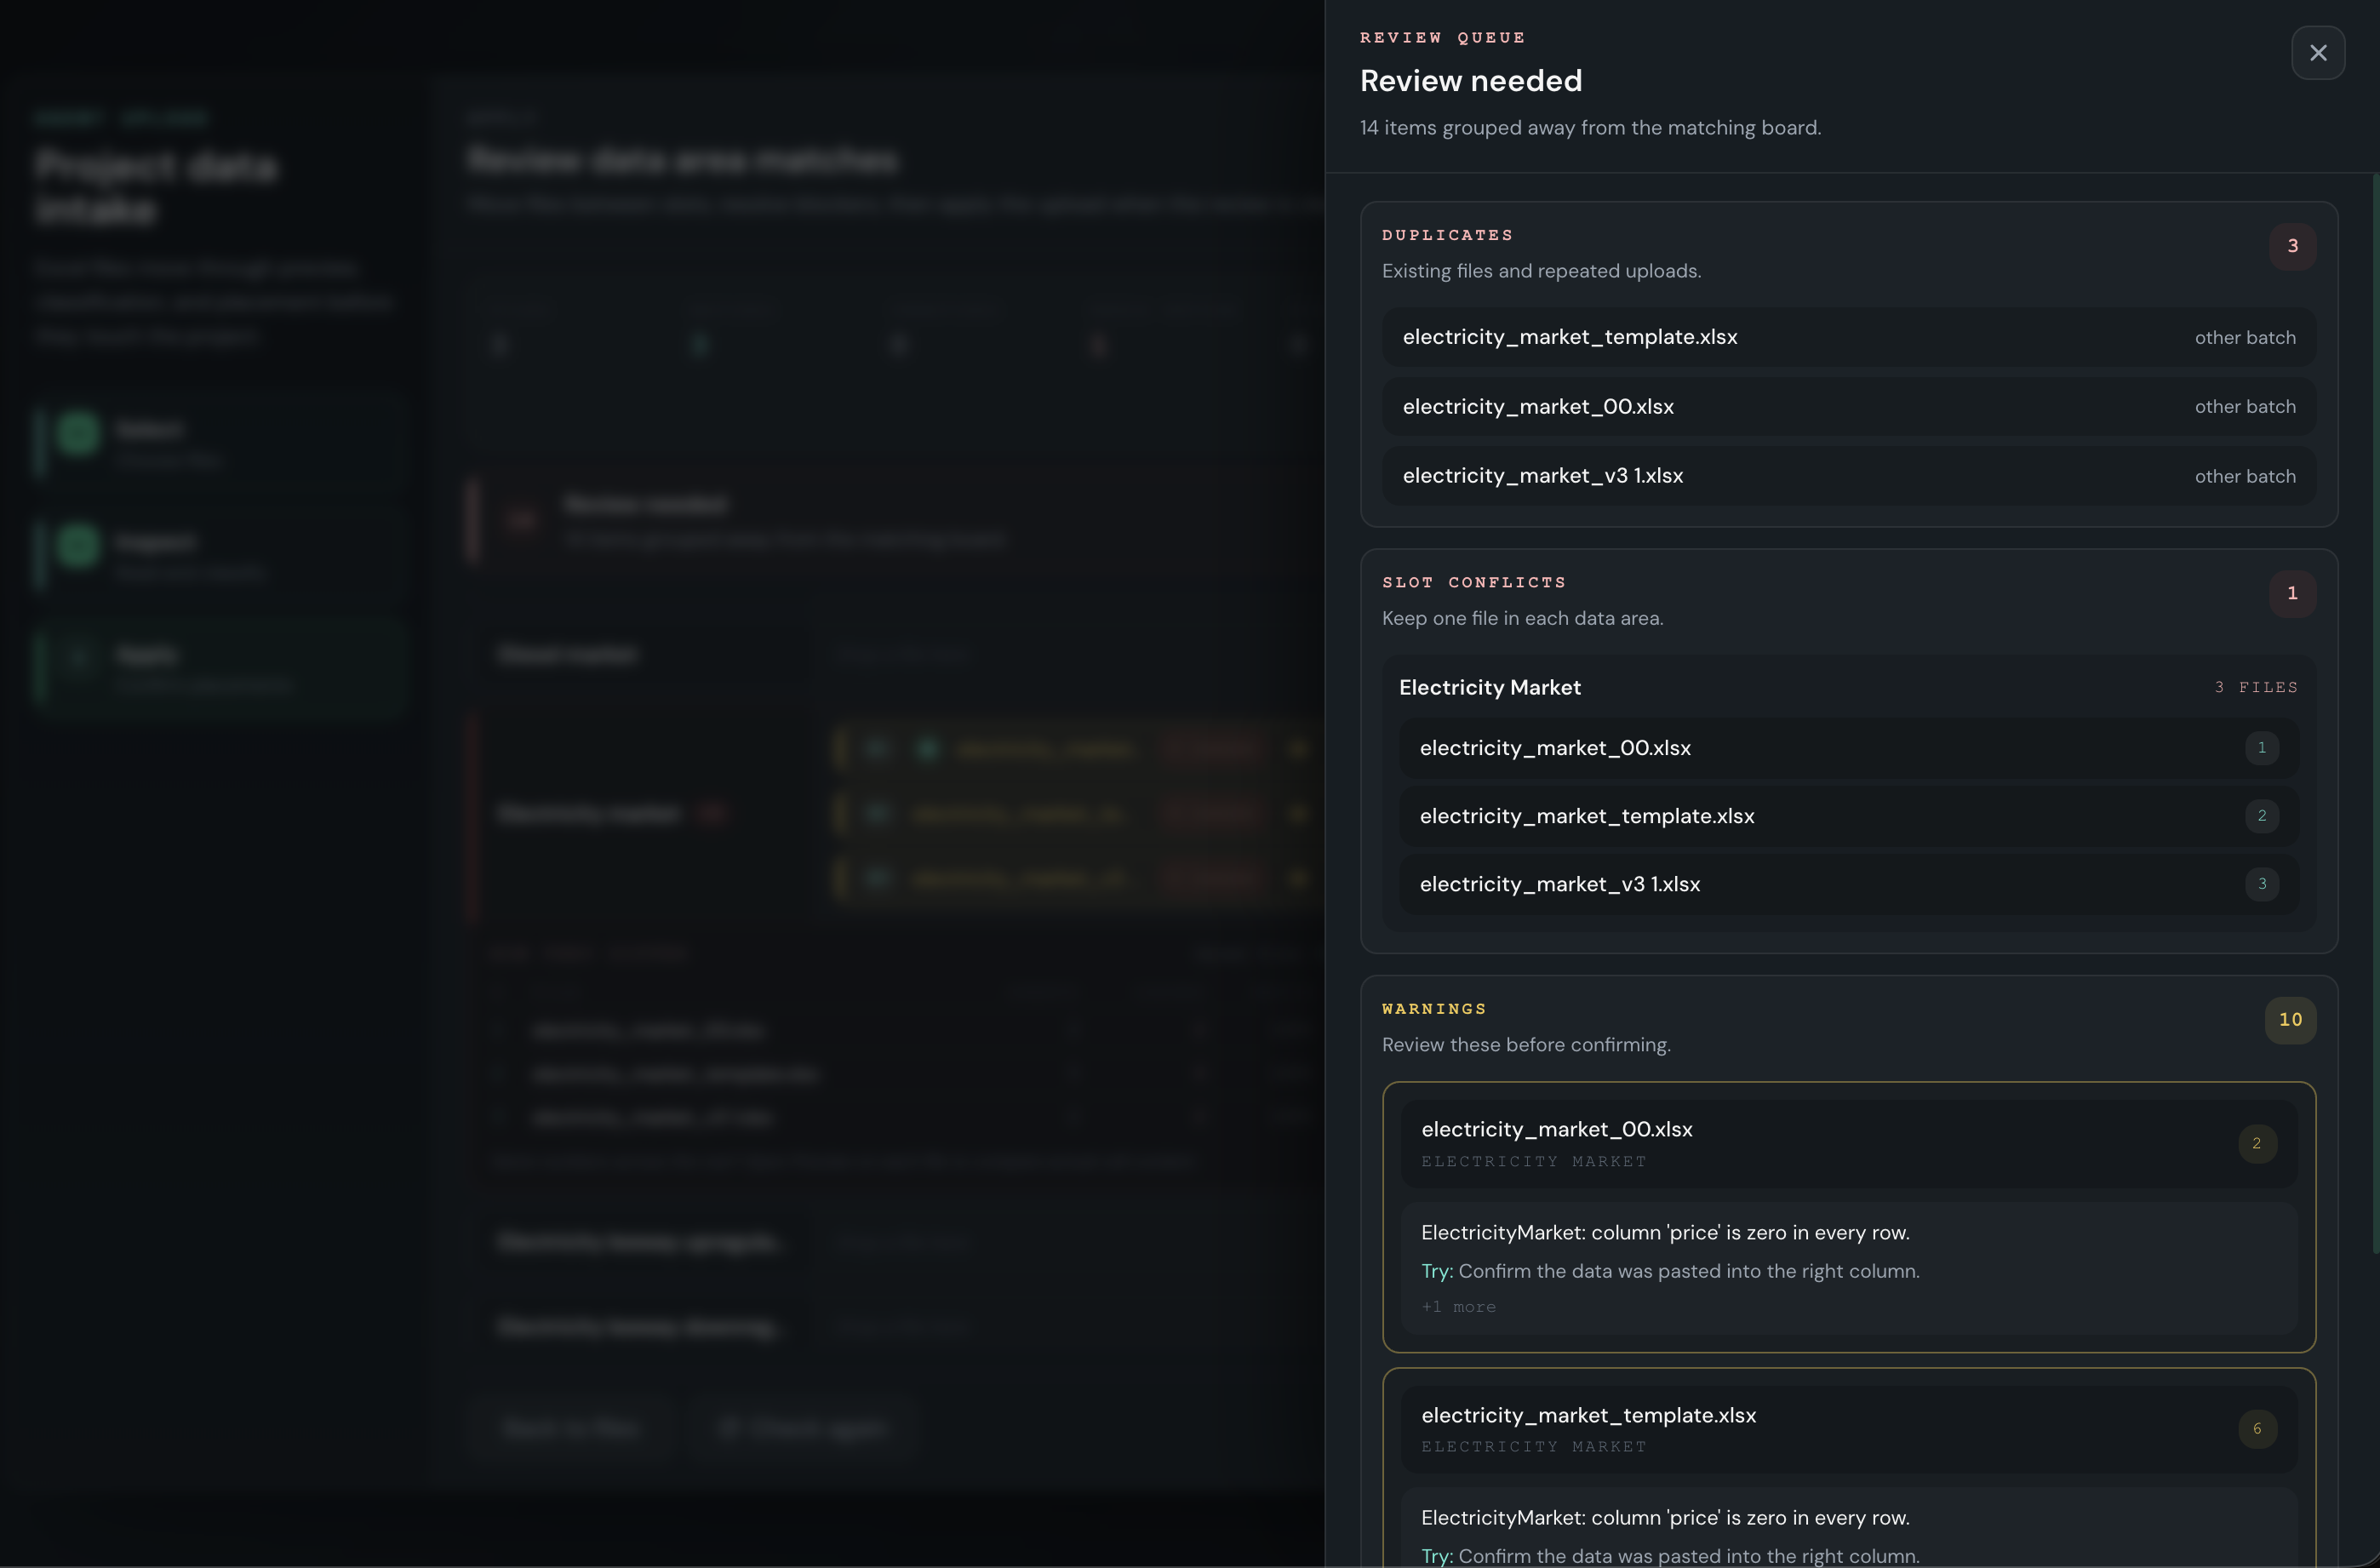
\includegraphics[width=0.9\linewidth]{Figures/chadi_review_queue.png}
  \caption{Review queue: duplicates, slot conflicts, and data-quality warnings to resolve.}
  \label{fig:impl-review}
\end{figure}

\subsection{Topology generation and parameter application}

The topology flow shows the assistant moving from explanation to proposal, with the
write path kept visible and approval-gated. Three responsibilities stay separate:
the agent interprets intent, the interface presents alternatives and pending
changes, and deterministic project state is updated only after confirmation
(Figures~\ref{fig:impl-topoexpl}--\ref{fig:impl-bulkchange}).

\begin{figure}[H]
  \centering
  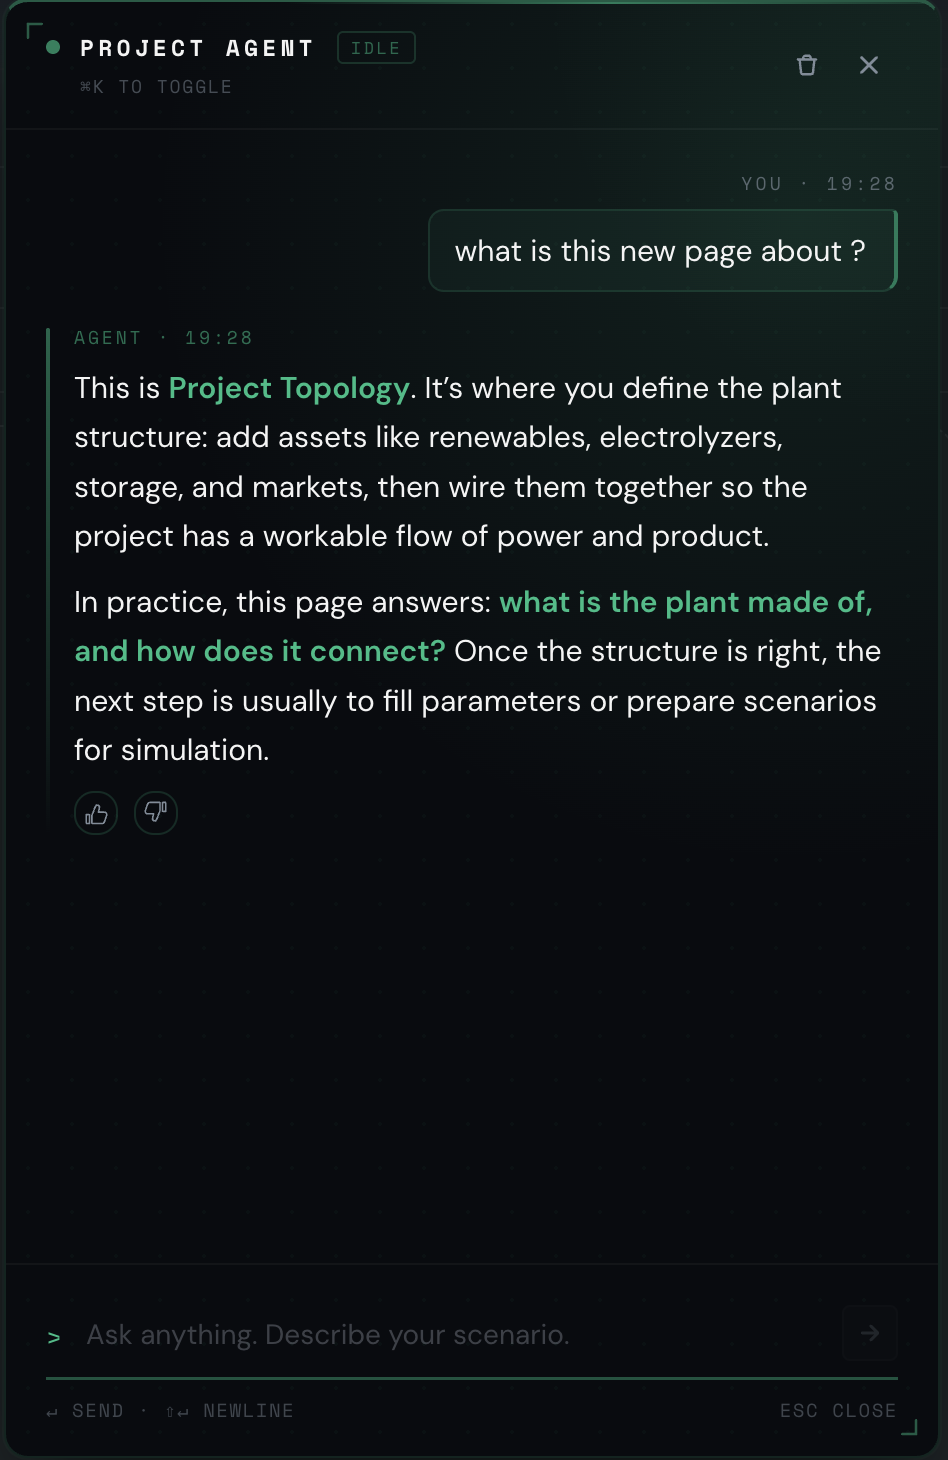
\includegraphics[width=0.48\linewidth]{Figures/chadi_topology_explanation.png}
  \caption{Topology explanation: the agent explains the graph before modifying it.}
  \label{fig:impl-topoexpl}
\end{figure}

\begin{figure}[H]
  \centering
  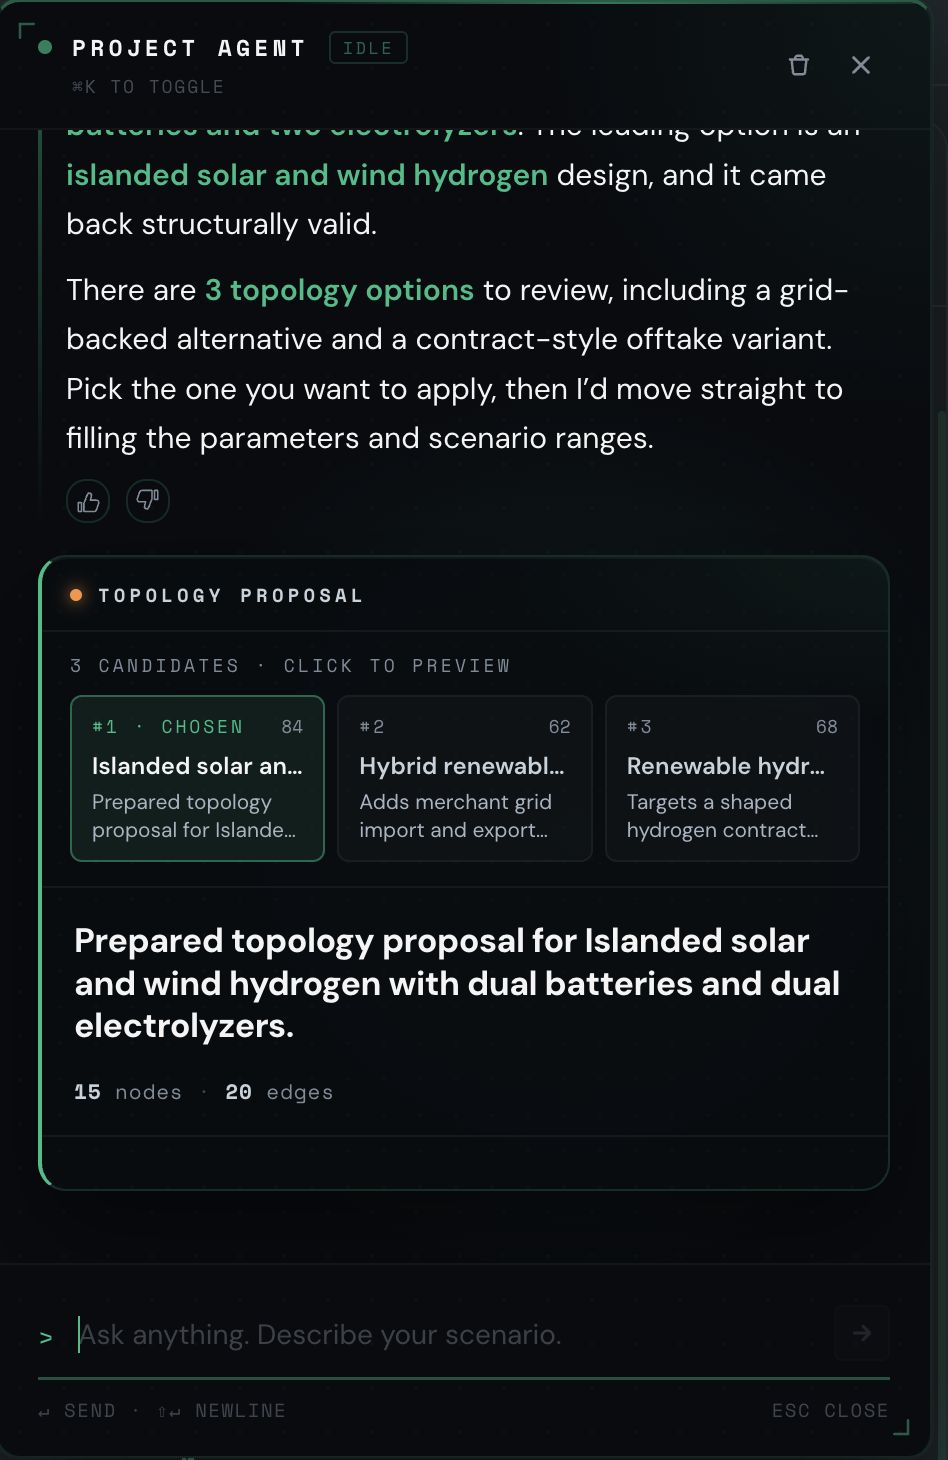
\includegraphics[width=0.48\linewidth]{Figures/chadi_topology_proposal.png}
  \caption{Topology proposal: candidate structures with a preferred option, for review.}
  \label{fig:impl-topoproposal}
\end{figure}

\begin{figure}[H]
  \centering
  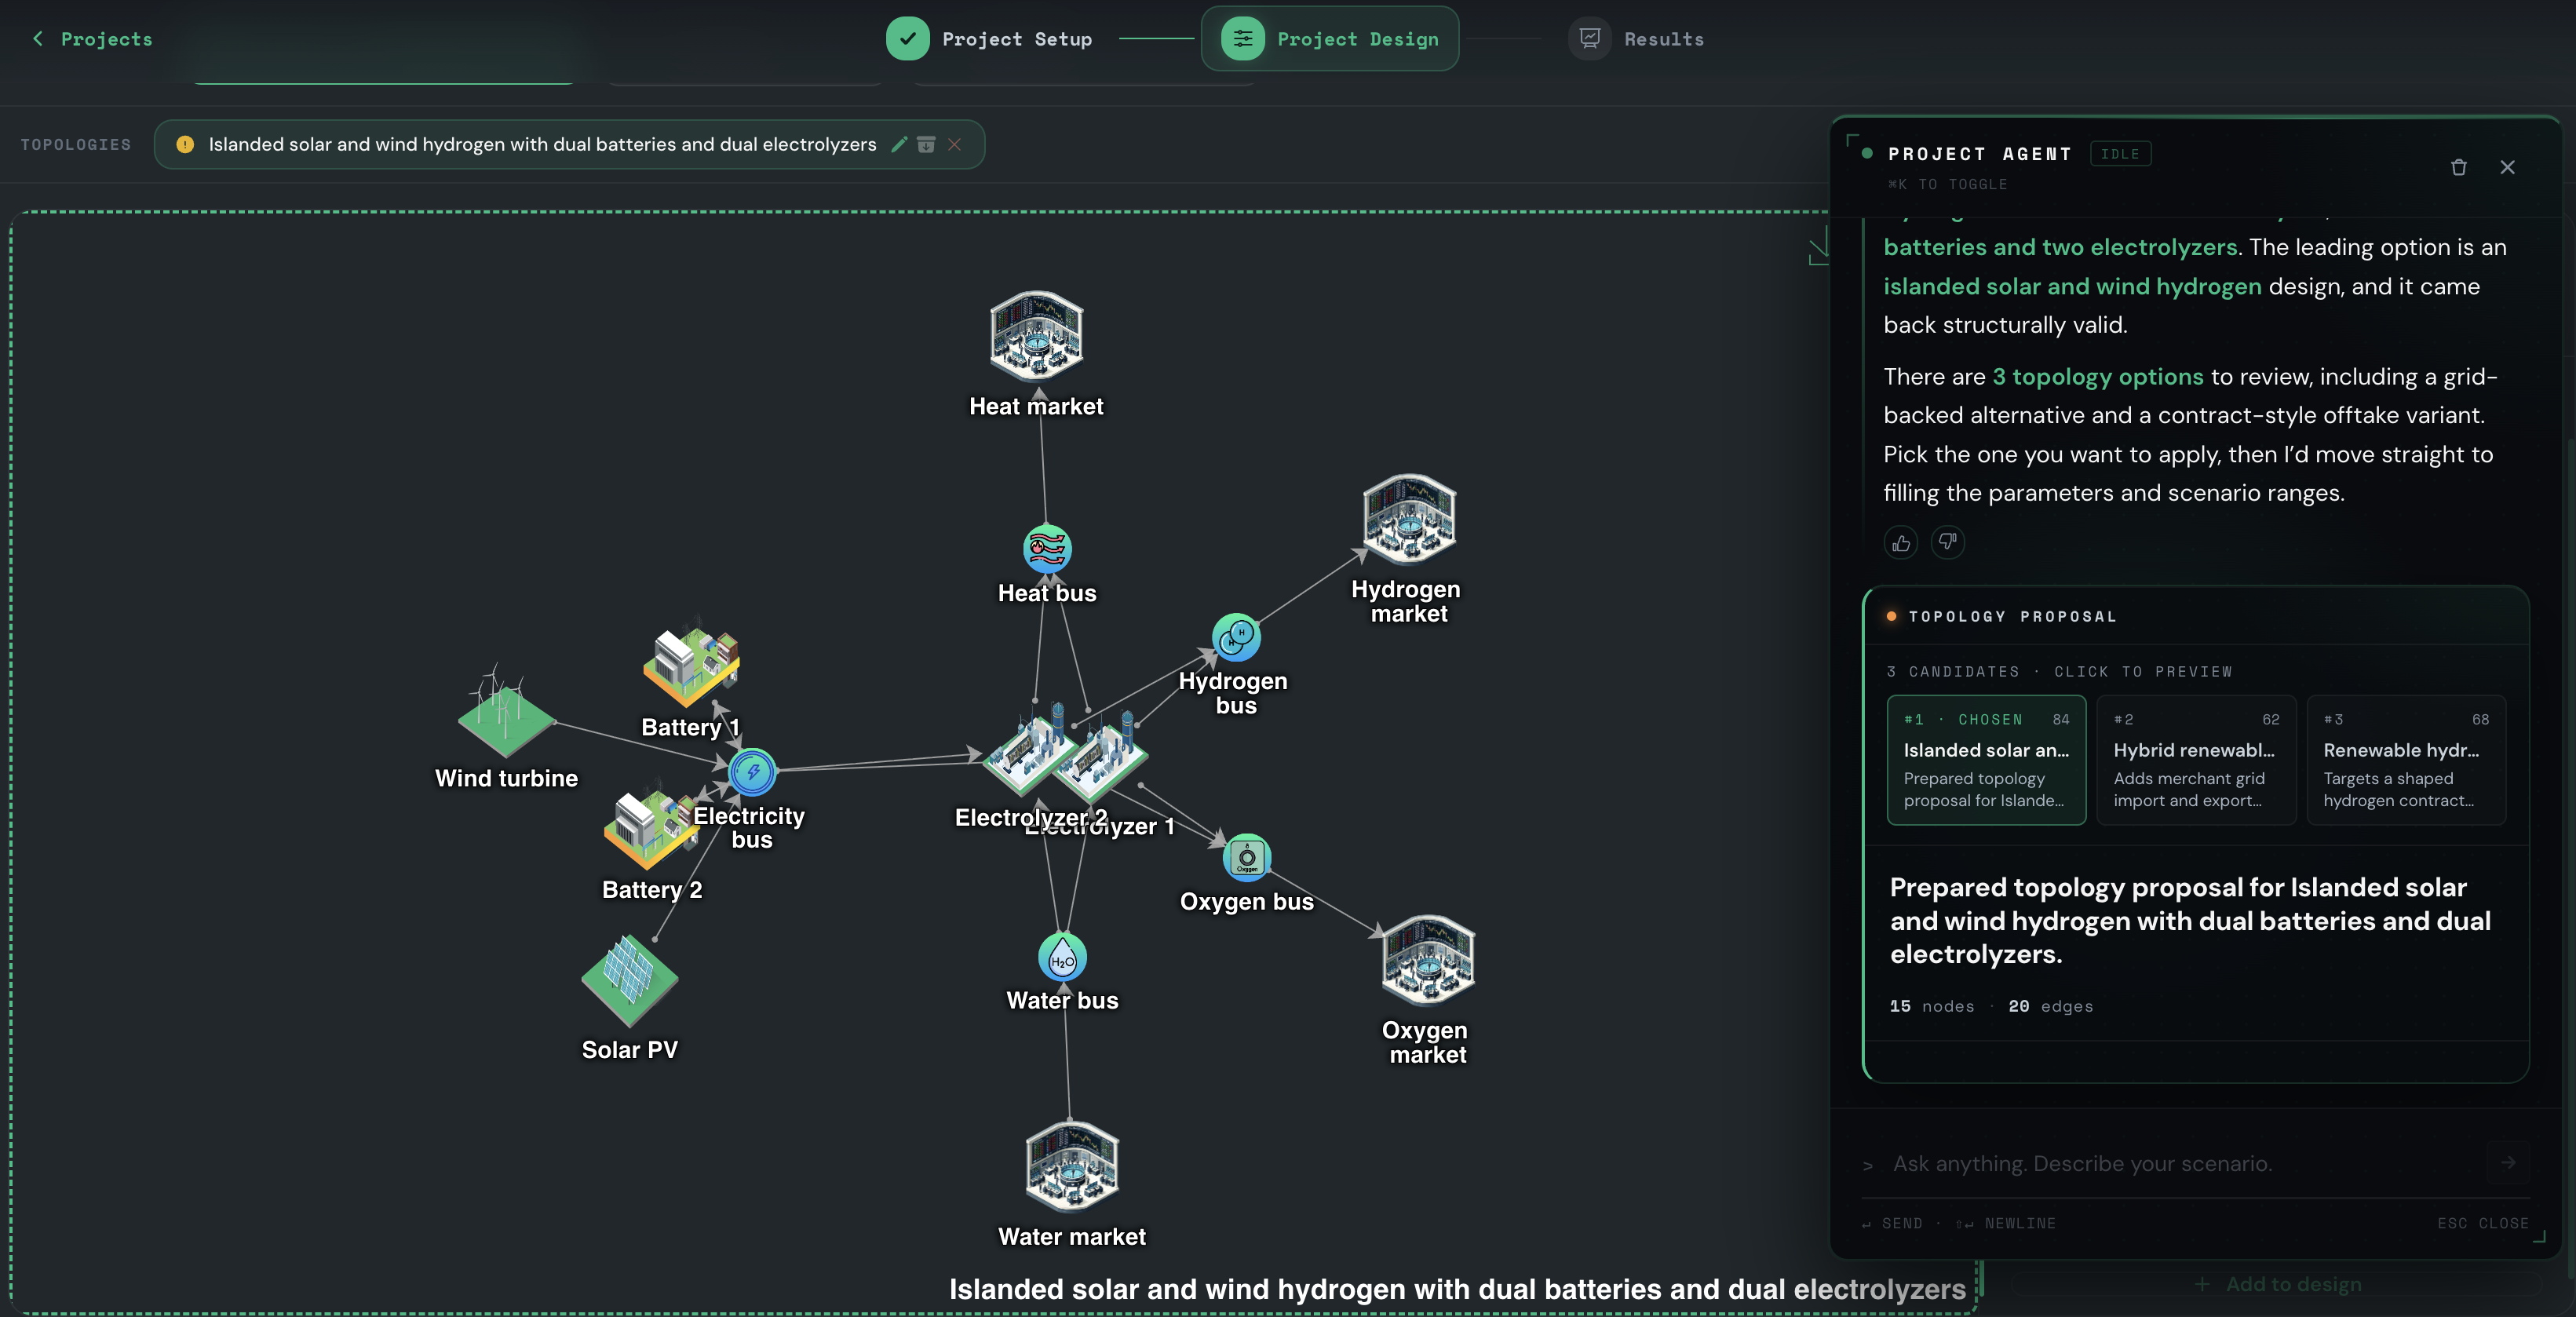
\includegraphics[width=0.95\linewidth]{Figures/chadi_generated_topology.png}
  \caption{Generated topology: the chosen structure appears on the canvas.}
  \label{fig:impl-gentopo}
\end{figure}

\begin{figure}[H]
  \centering
  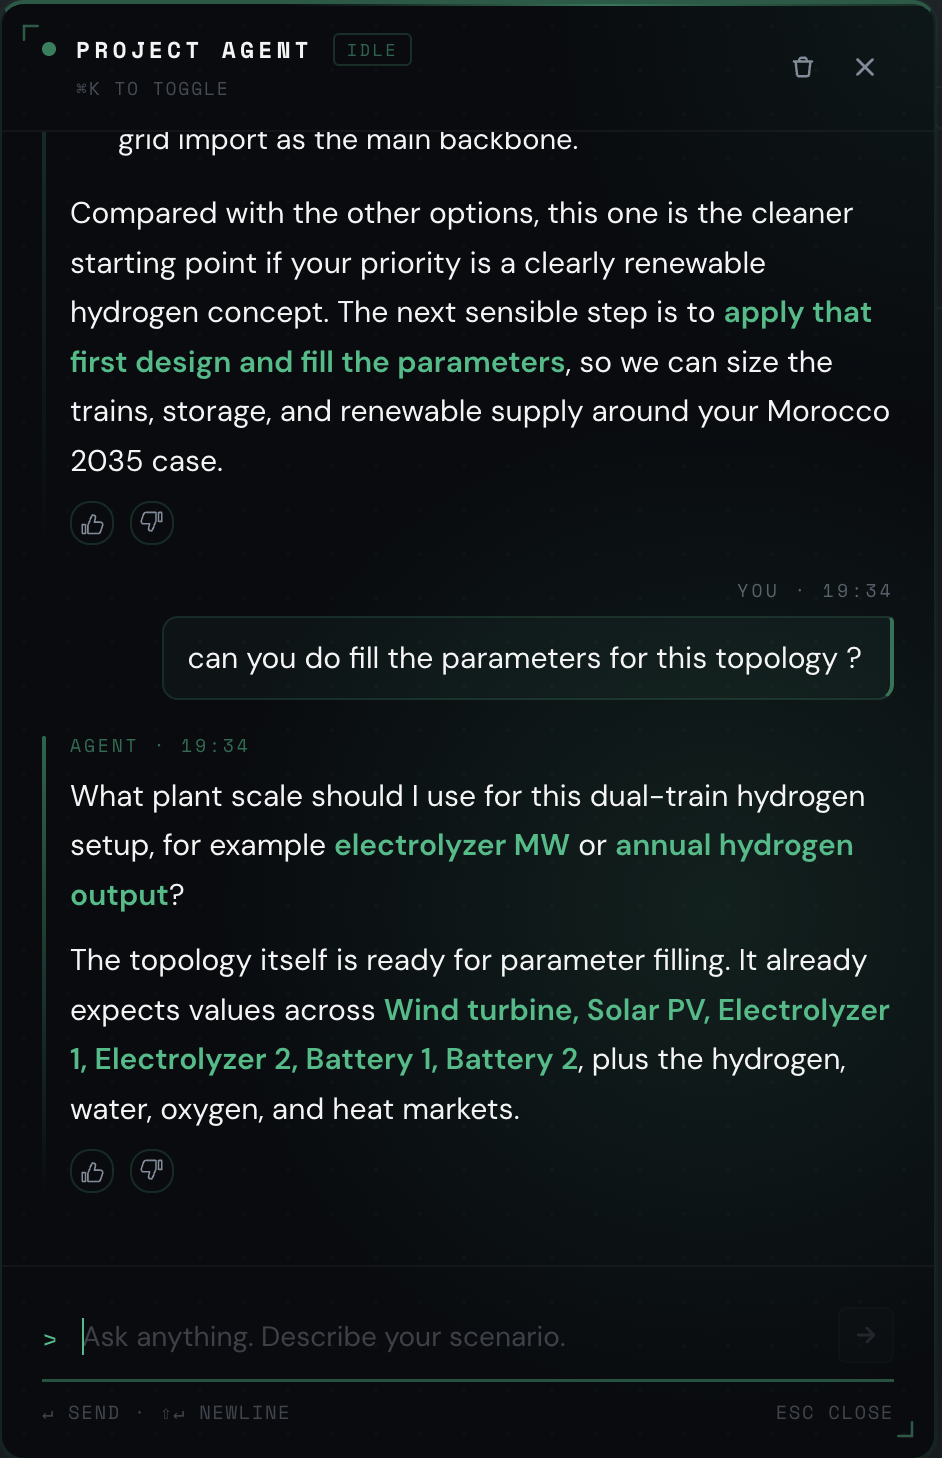
\includegraphics[width=0.48\linewidth]{Figures/chadi_missing_parameter.png}
  \caption{Missing parameter: the agent asks for a key sizing input rather than inventing it.}
  \label{fig:impl-missingparam}
\end{figure}

\begin{figure}[H]
  \centering
  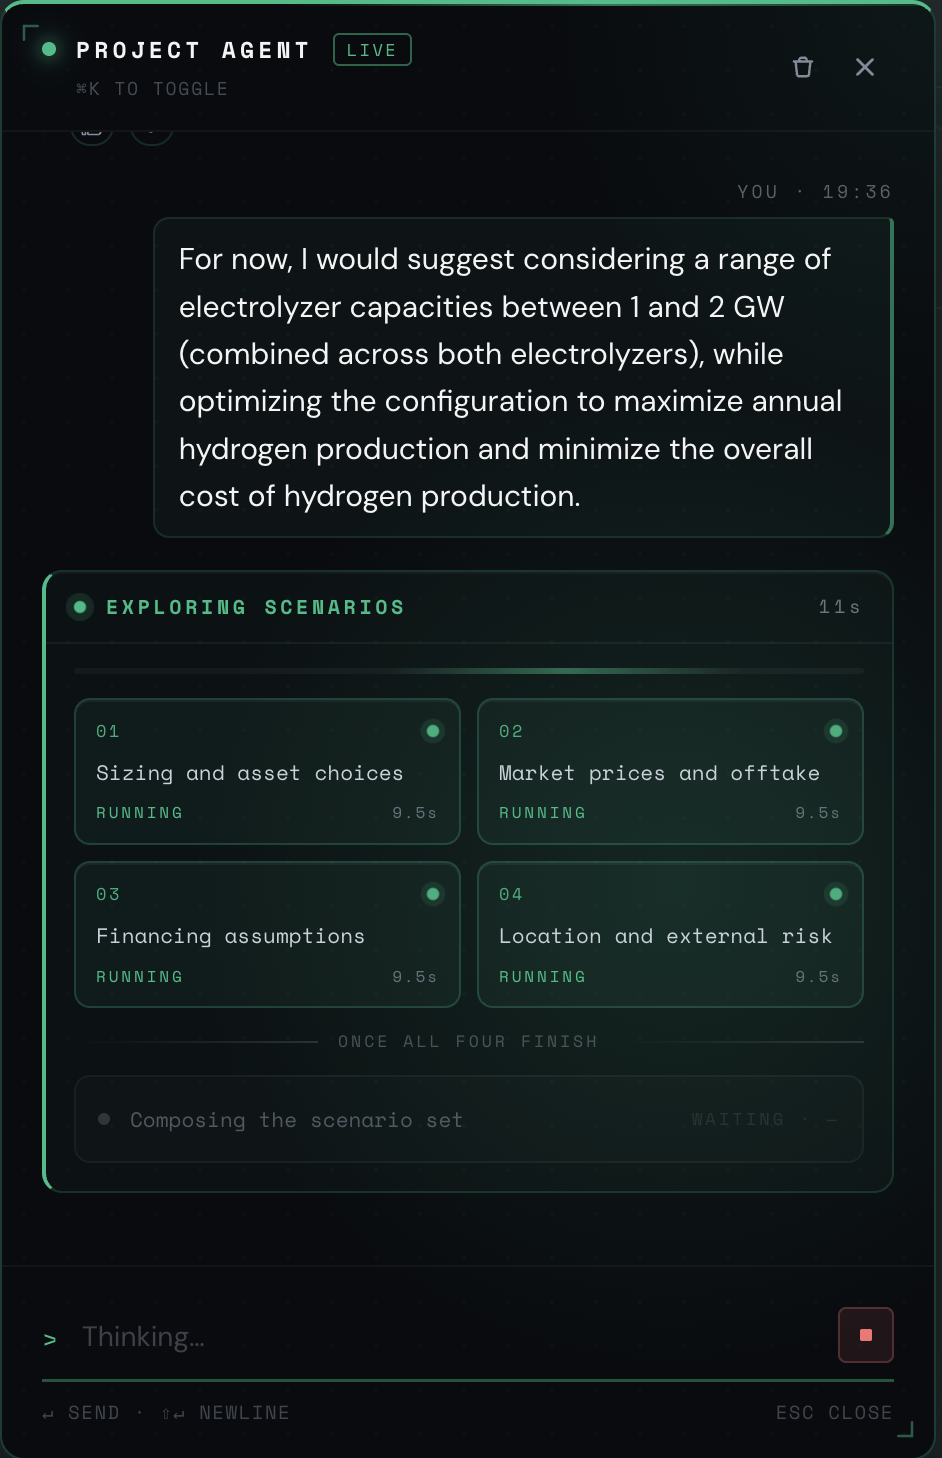
\includegraphics[width=0.48\linewidth]{Figures/chadi_scenario_cards.png}
  \caption{Scenario cards: study directions turned into a manageable sweep.}
  \label{fig:impl-scenariocards}
\end{figure}

\begin{figure}[H]
  \centering
  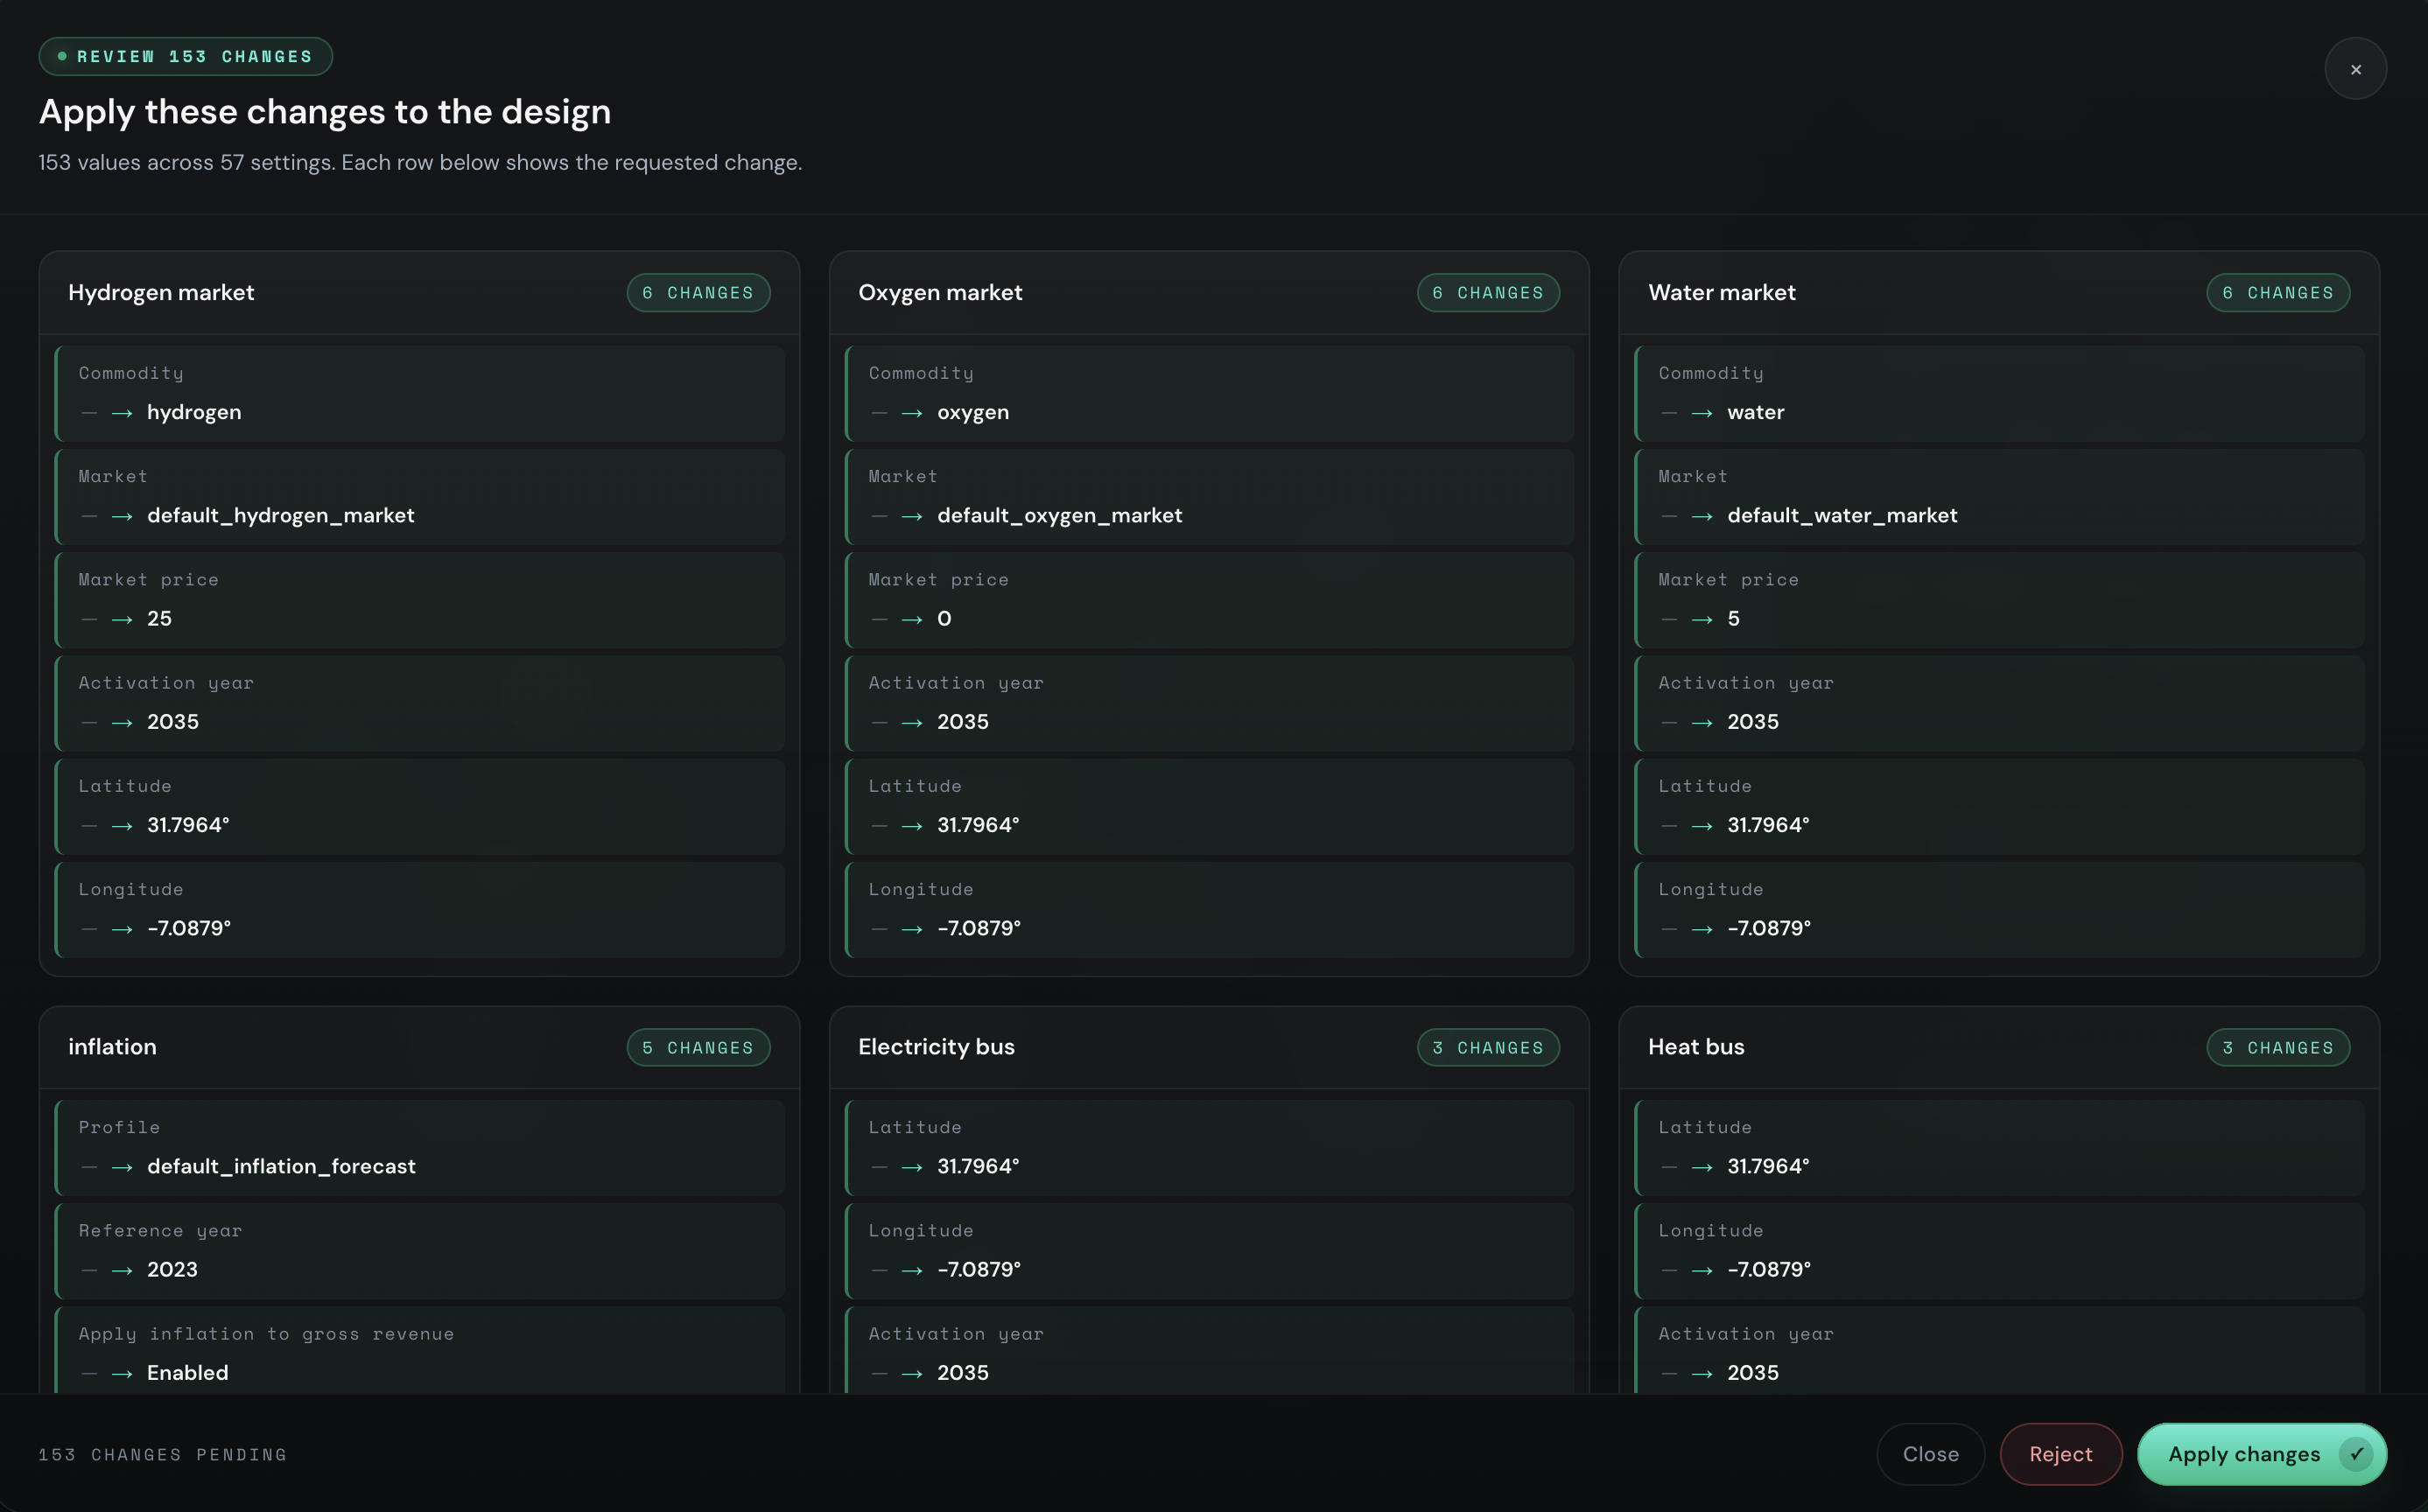
\includegraphics[width=0.9\linewidth]{Figures/chadi_bulk_change.png}
  \caption{Bulk change review: proposed values grouped by entity, auditable before applying.}
  \label{fig:impl-bulkchange}
\end{figure}

\subsection{Result exploration and interpretation}
\label{sec:impl-results}

The final stage of the journey is result exploration and
interpretation. Once a grid search has completed, its population of
simulations is explored through an interactive results view built as a set of
components over the deterministic outputs, organized so that a user moves from
comparing a whole population of runs, to reading one run in depth, to asking for an
explanation of exactly what is on screen.

Runs are first browsed and managed in a results library, with live status, search,
download, and cancellation (Figure~\ref{fig:impl-library}). The chart view is the
analytical core: a scatter with selectable axes plots one point per simulation and
makes trade-offs and standout runs immediately visible, with dense tables for exact
comparison (Figure~\ref{fig:impl-scatter}). Selecting a run opens a six-panel
operational dashboard that tells that run's operational money story, governed by a
time-filter sidebar (Figure~\ref{fig:impl-dashboard}). The financial output is
rendered as a grouped, expandable discounted-cash-flow table with drill-down to
per-asset and per-market components, amortization and debt groups, reconciliation,
payback highlighting, and hover-for-exact-figure (Figure~\ref{fig:impl-dcf}). From
any chart or run, the analyst can ask the interpreter to explain what is shown; the
agent streams a plain-language narration and a set of insight cards, citing only
figures read from the deterministic output, and can embed the chart it refers to
(Figure~\ref{fig:impl-interp}); further interpretation examples are shown in
Figure~\ref{fig:impl-interp-examples}.

\begin{figure}[H]
  \centering
  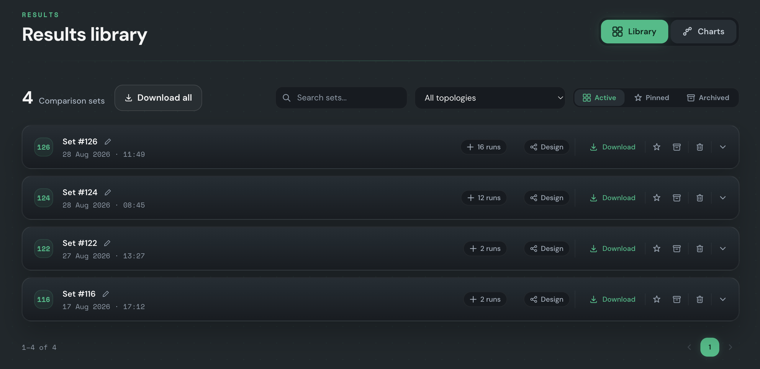
\includegraphics[width=0.95\linewidth]{Figures/impl_library.png}
  \caption{The results library: run management with status, search, and per-run actions.}
  \label{fig:impl-library}
\end{figure}

\begin{figure}[H]
  \centering
  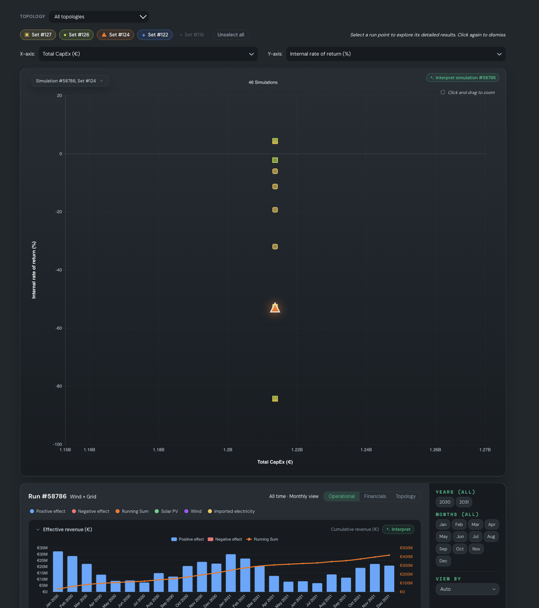
\includegraphics[width=0.72\linewidth]{Figures/impl_scatter.png}
  \caption{Interactive results exploration: a scatter with selectable axes and interpret-on-demand.}
  \label{fig:impl-scatter}
\end{figure}

\begin{figure}[H]
  \centering
  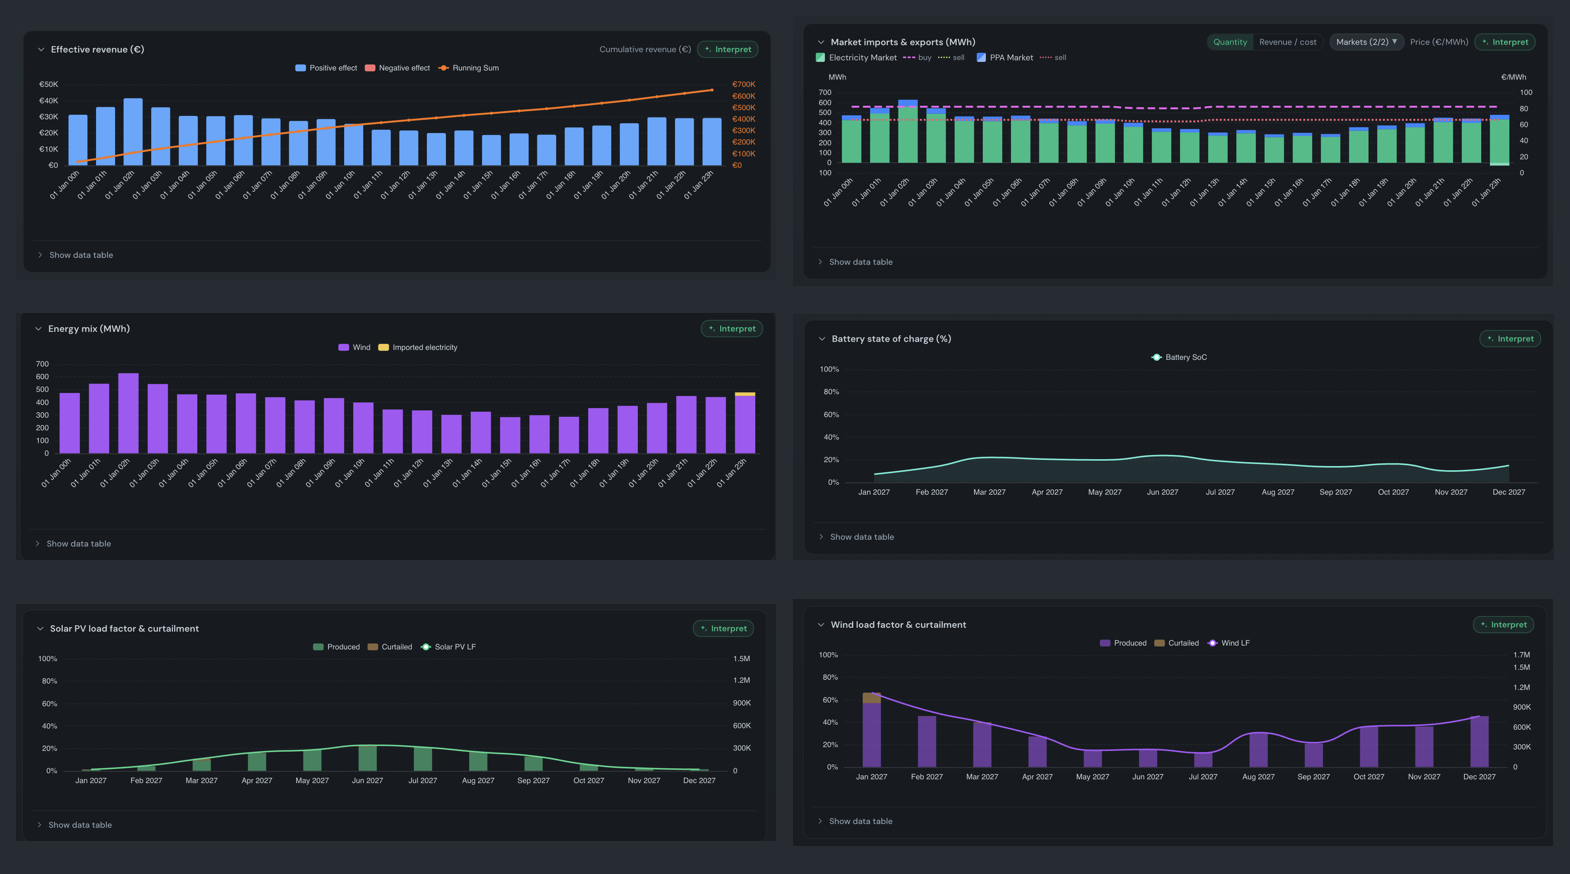
\includegraphics[width=\linewidth]{Figures/impl_dashboard.png}
  \caption{The per-run operational dashboard: the six-panel operational money story.}
  \label{fig:impl-dashboard}
\end{figure}

\begin{figure}[H]
  \centering
  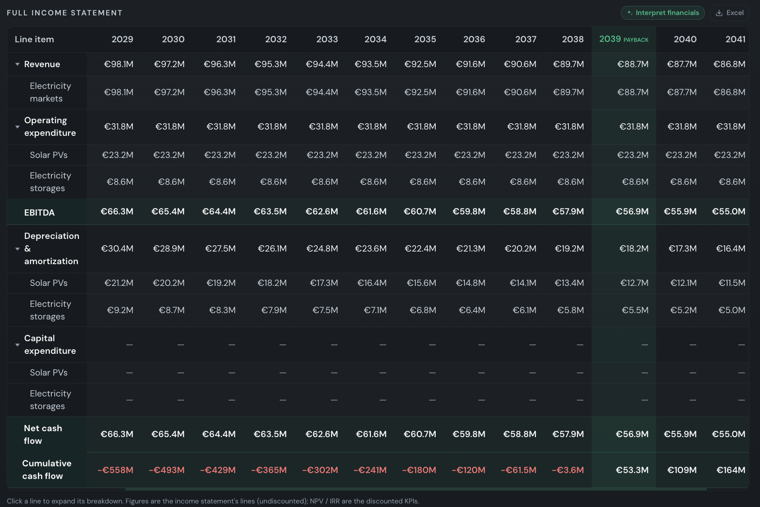
\includegraphics[width=0.92\linewidth]{Figures/impl_dcf.png}
  \caption{Navigable discounted-cash-flow table with drill-down and payback highlighting.}
  \label{fig:impl-dcf}
\end{figure}

\begin{figure}[H]
  \centering
  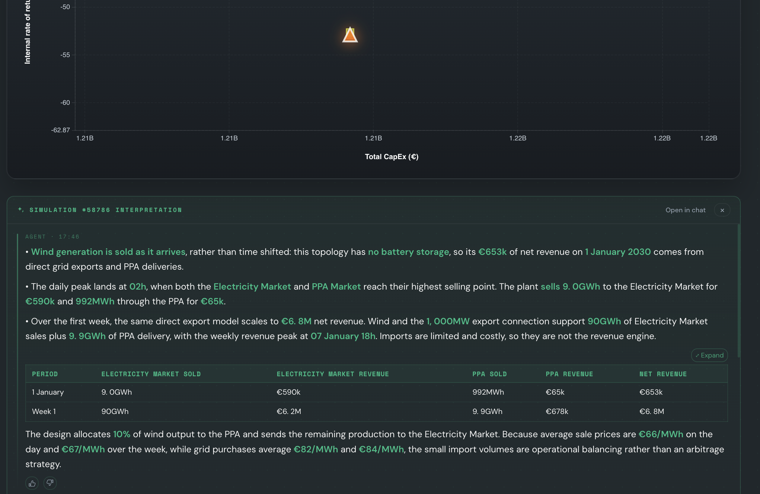
\includegraphics[width=0.8\linewidth]{Figures/impl_interp.png}
  \caption{Grounded, streamed interpretation of a run, with insight cards and the referenced chart.}
  \label{fig:impl-interp}
\end{figure}


\begin{figure}[H]
  \centering
  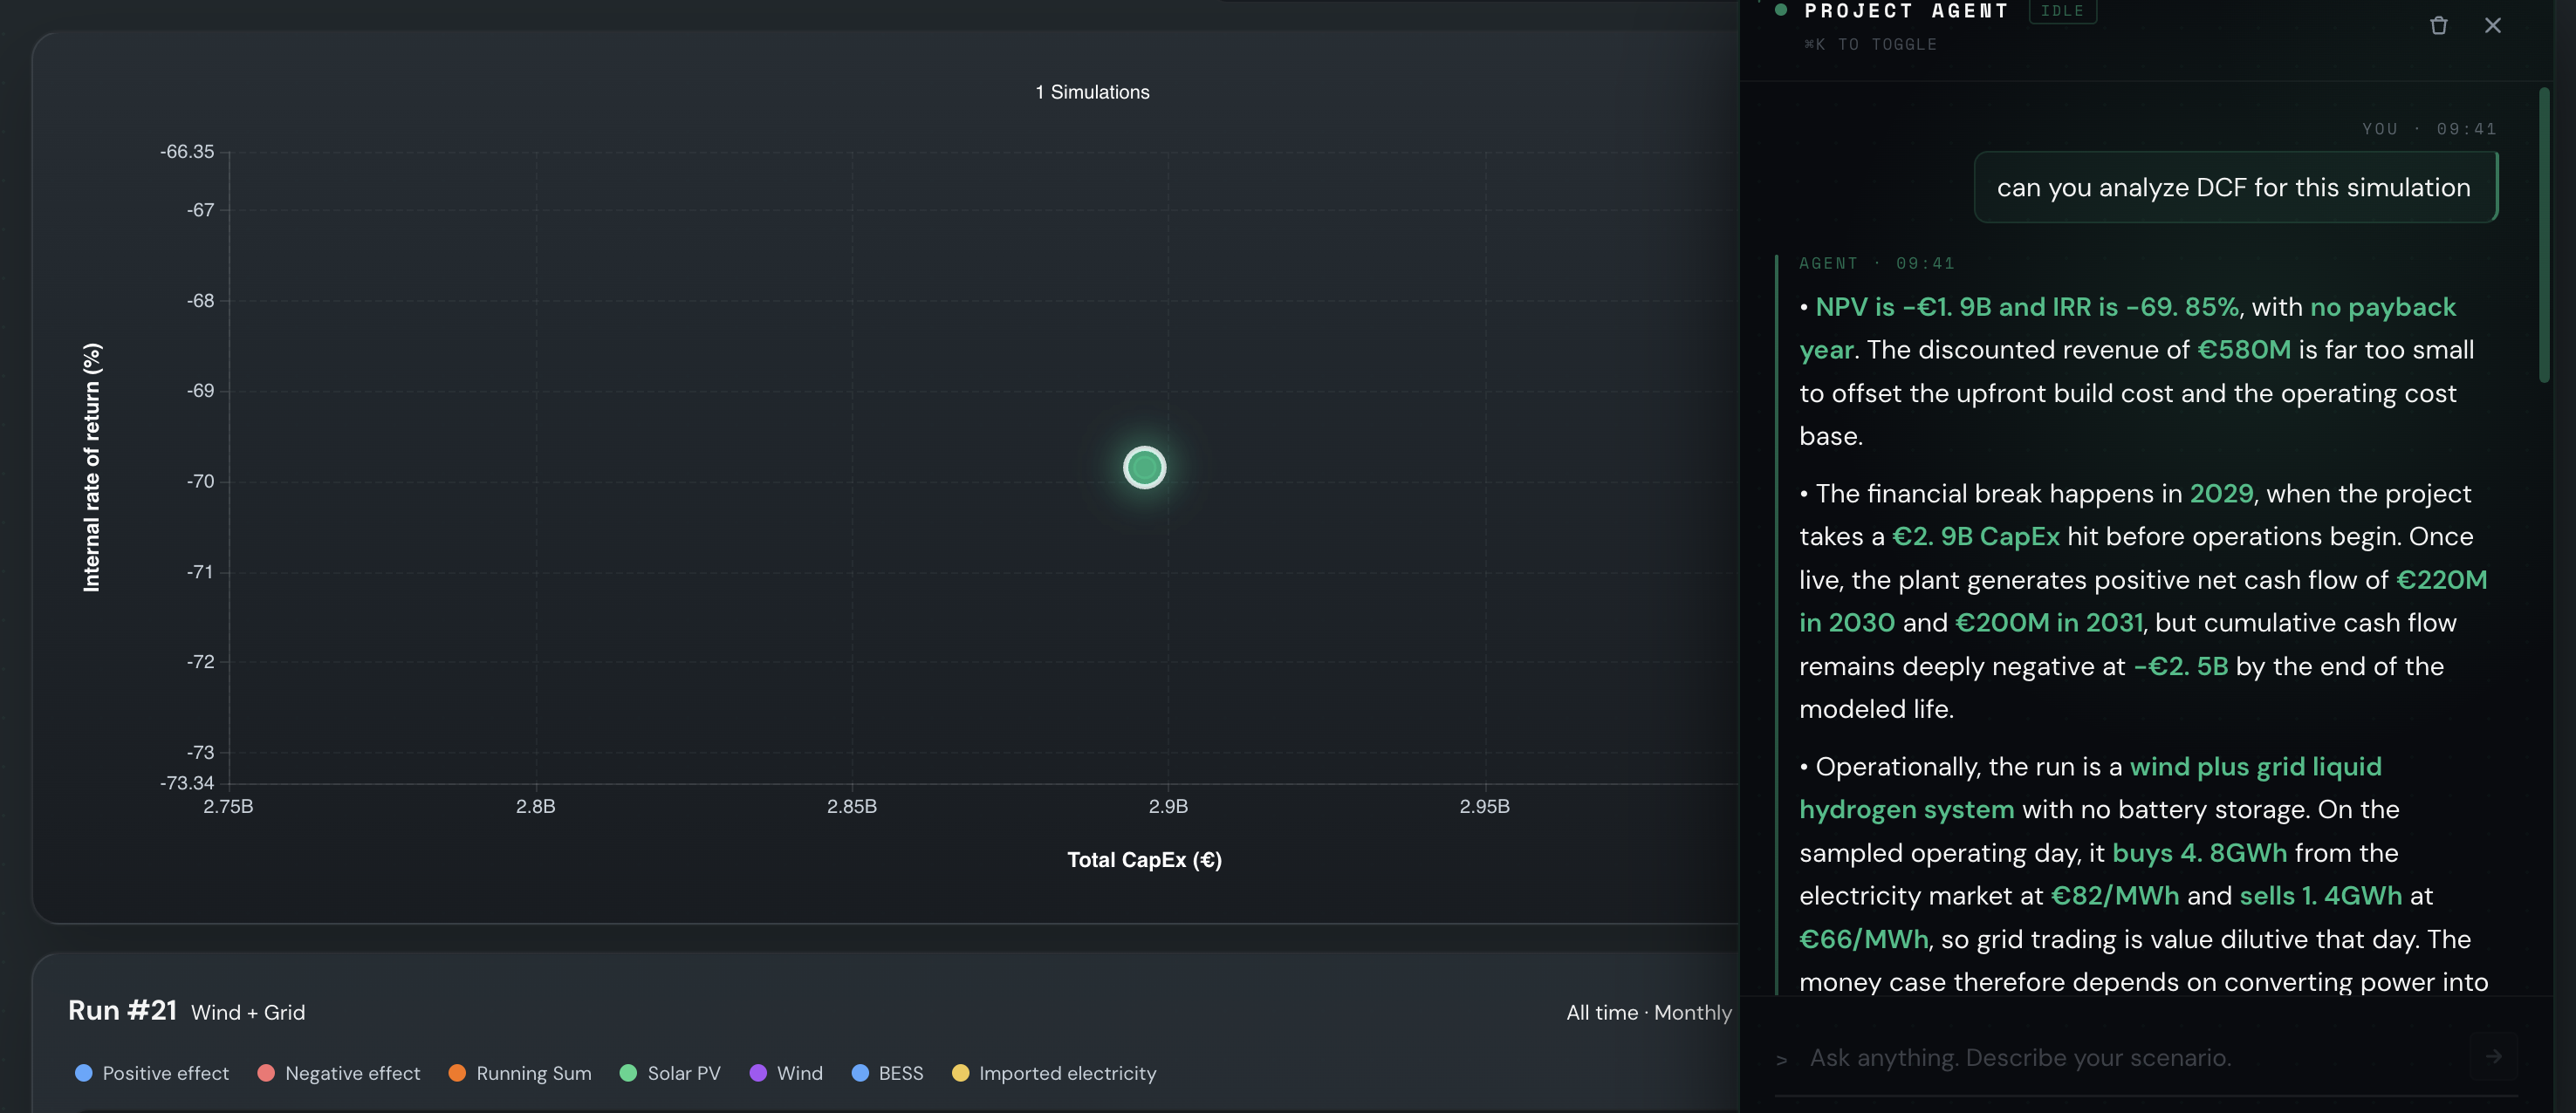
\includegraphics[width=0.64\linewidth]{Figures/image (19).png}\\[0.15cm]
  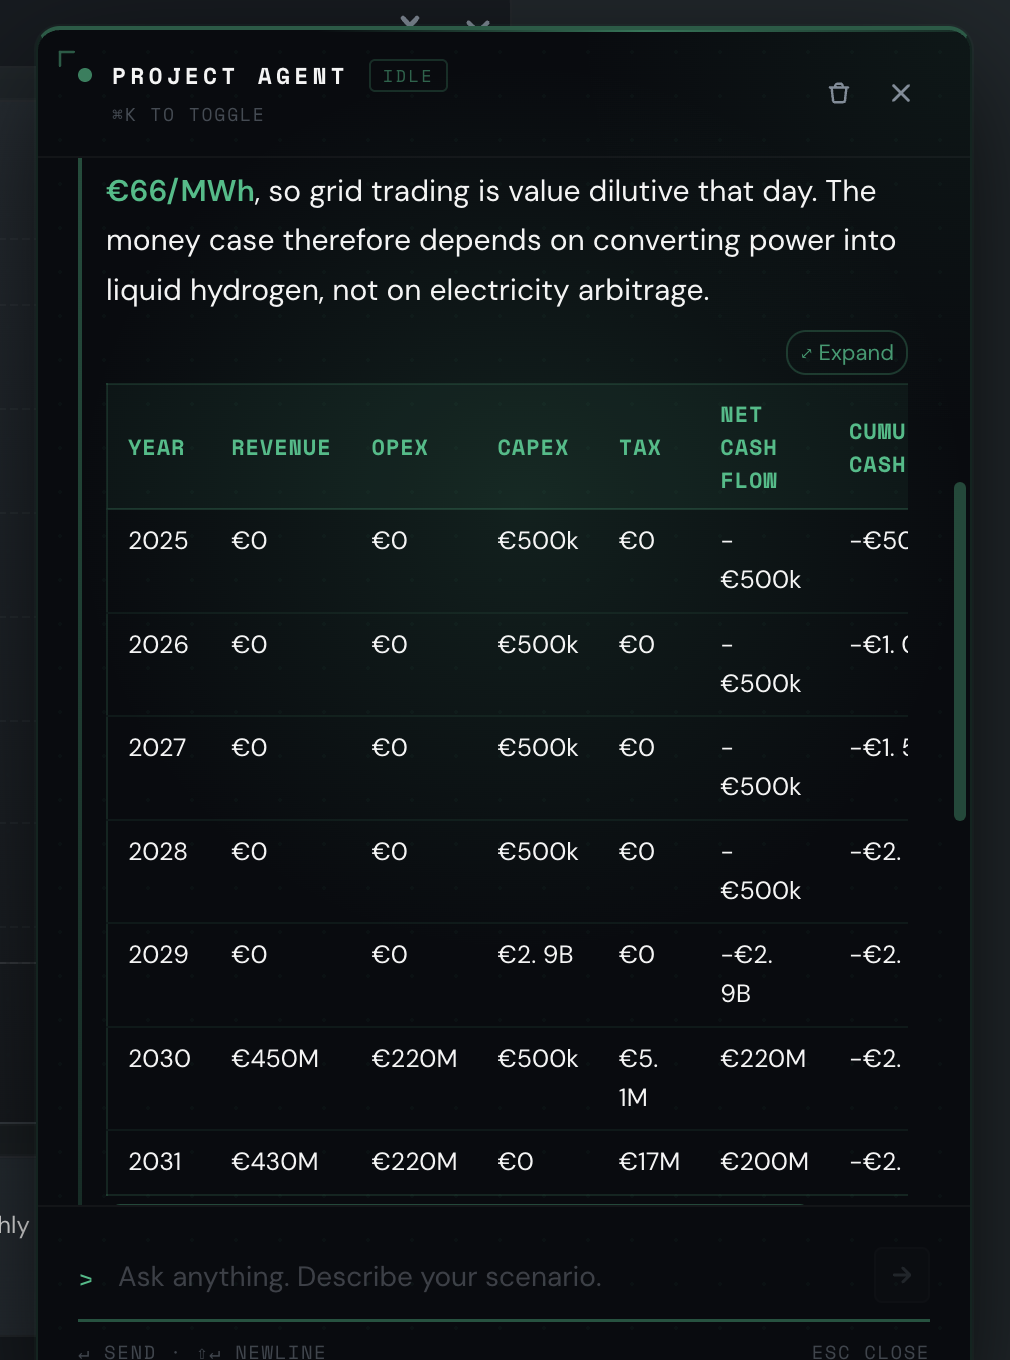
\includegraphics[width=0.3\linewidth]{Figures/image (20).png}
  \hspace{0.04\linewidth}
  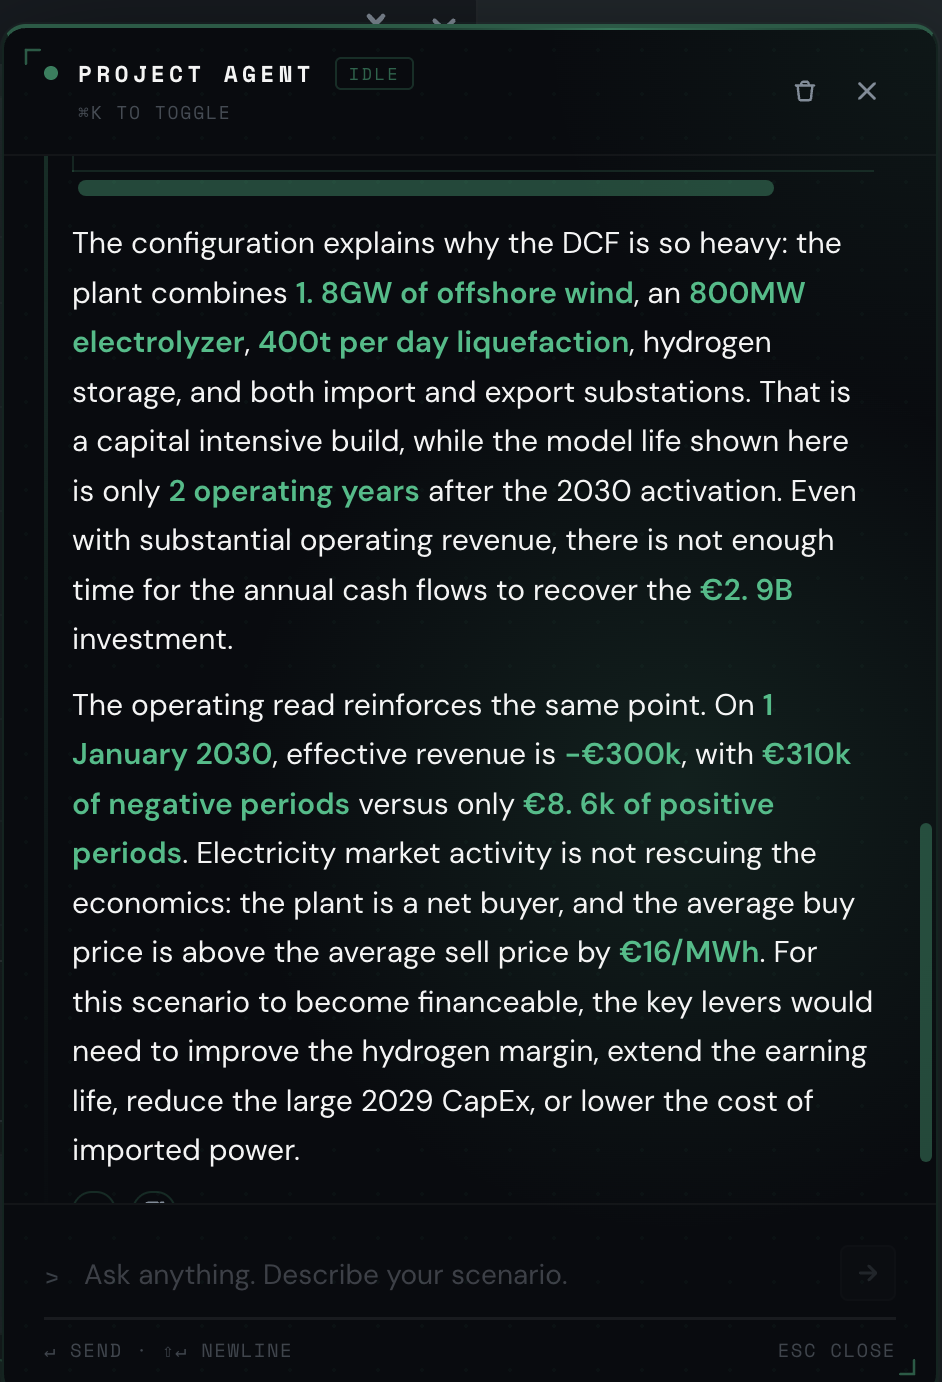
\includegraphics[width=0.3\linewidth]{Figures/image (22).png}
  \caption{Interpretation examples: a run analyzed beside its scatter (top), and,
    within the chat, an embedded discounted-cash-flow table and a grounded
    narrative citing deterministic figures (bottom).}
  \label{fig:impl-interp-examples}
\end{figure}

\newpage

In the delivered system these capabilities are shipped, not prototypes. The
interpreter runs on the separate agent runtime and is exposed as a single Director
tool (Figure~\ref{fig:impl-interp-arch}), so a user reaches it from the same chat
that drives the rest of the workflow; each explanation is a fresh, grounded turn
streamed token by token into an inline block beneath the exact chart it describes.
The scatter, the operational dashboard, the discounted-cash-flow table, and the
interpreter all read the \textbf{same pure, unit-tested analytics}, so the figures a
written explanation cites cannot differ from the figures a chart plots. The result
is that a non-specialist can move from a population of runs, to one run's
operational and financial story, to a grounded answer about what it means, without
leaving the results page and without any number originating from the model.

\begin{figure}[H]
  \centering
  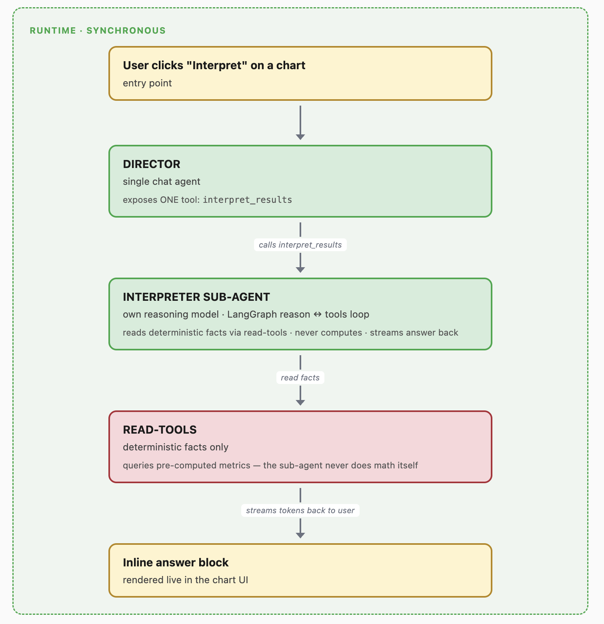
\includegraphics[width=0.6\linewidth]{Figures/impl_interp_arch.png}
  \caption{The implemented interpreter architecture: the Director exposes it as one read-only reason-and-tools loop.}
  \label{fig:impl-interp-arch}
\end{figure}

\section{Platform and operations implementation}
\label{sec:impl-ops}

The analytical experience runs on the restored platform. This section reports the
surrounding platform and operations work, from enterprise access to observability.

\subsection{Enterprise access verification}

Access is routed through the enterprise identity flow: the sign-in path redirects
users to the organization-managed verification screen before returning
authenticated traffic to the application (Figure~\ref{fig:impl-okta}). This confirms
that authentication was moved out of the product runtime and into the
organization-controlled identity path.

\begin{figure}[H]
  \centering
  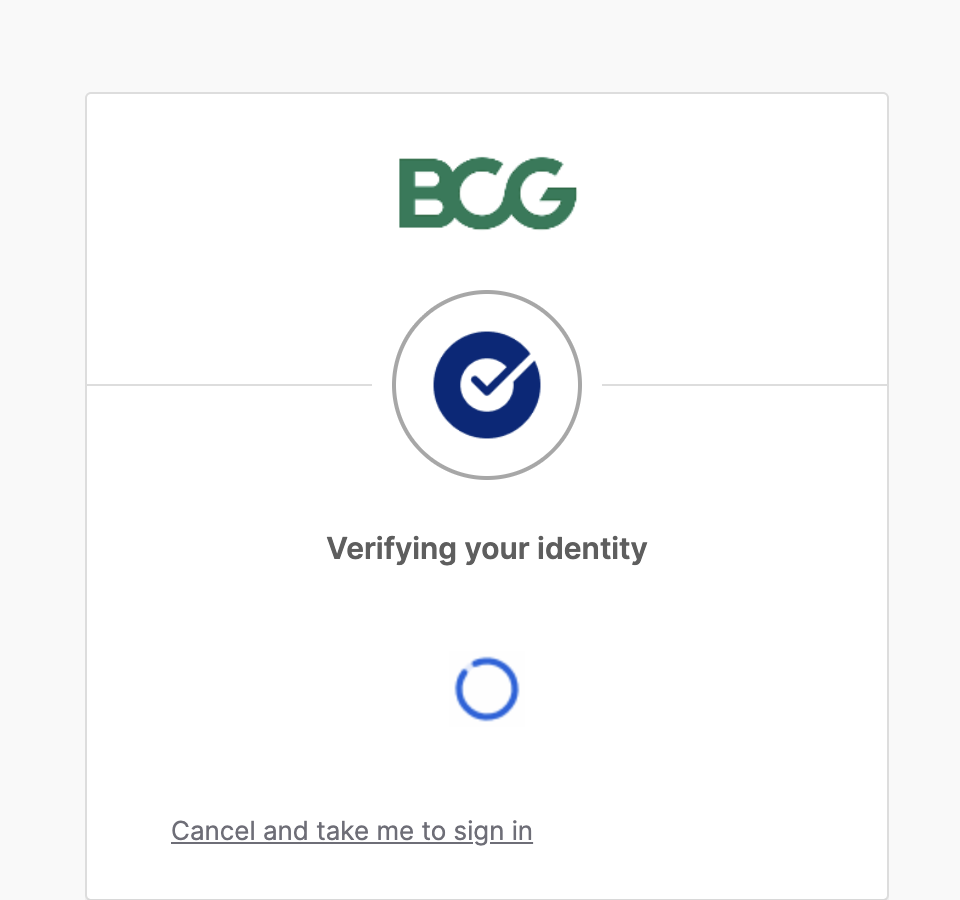
\includegraphics[width=0.5\linewidth]{Figures/chadi_okta.png}
  \caption{Enterprise identity verification: sign-in before reaching the application.}
  \label{fig:impl-okta}
\end{figure}

\subsection{Deployment and infrastructure delivery}

The restored delivery chain shows that the product can move from a code change to a
controlled deployment again: application changes pass through continuous-integration
workflows and infrastructure changes are applied through infrastructure-as-code
(Figures~\ref{fig:impl-circleci} and~\ref{fig:impl-terraform}).

\begin{figure}[H]
  \centering
  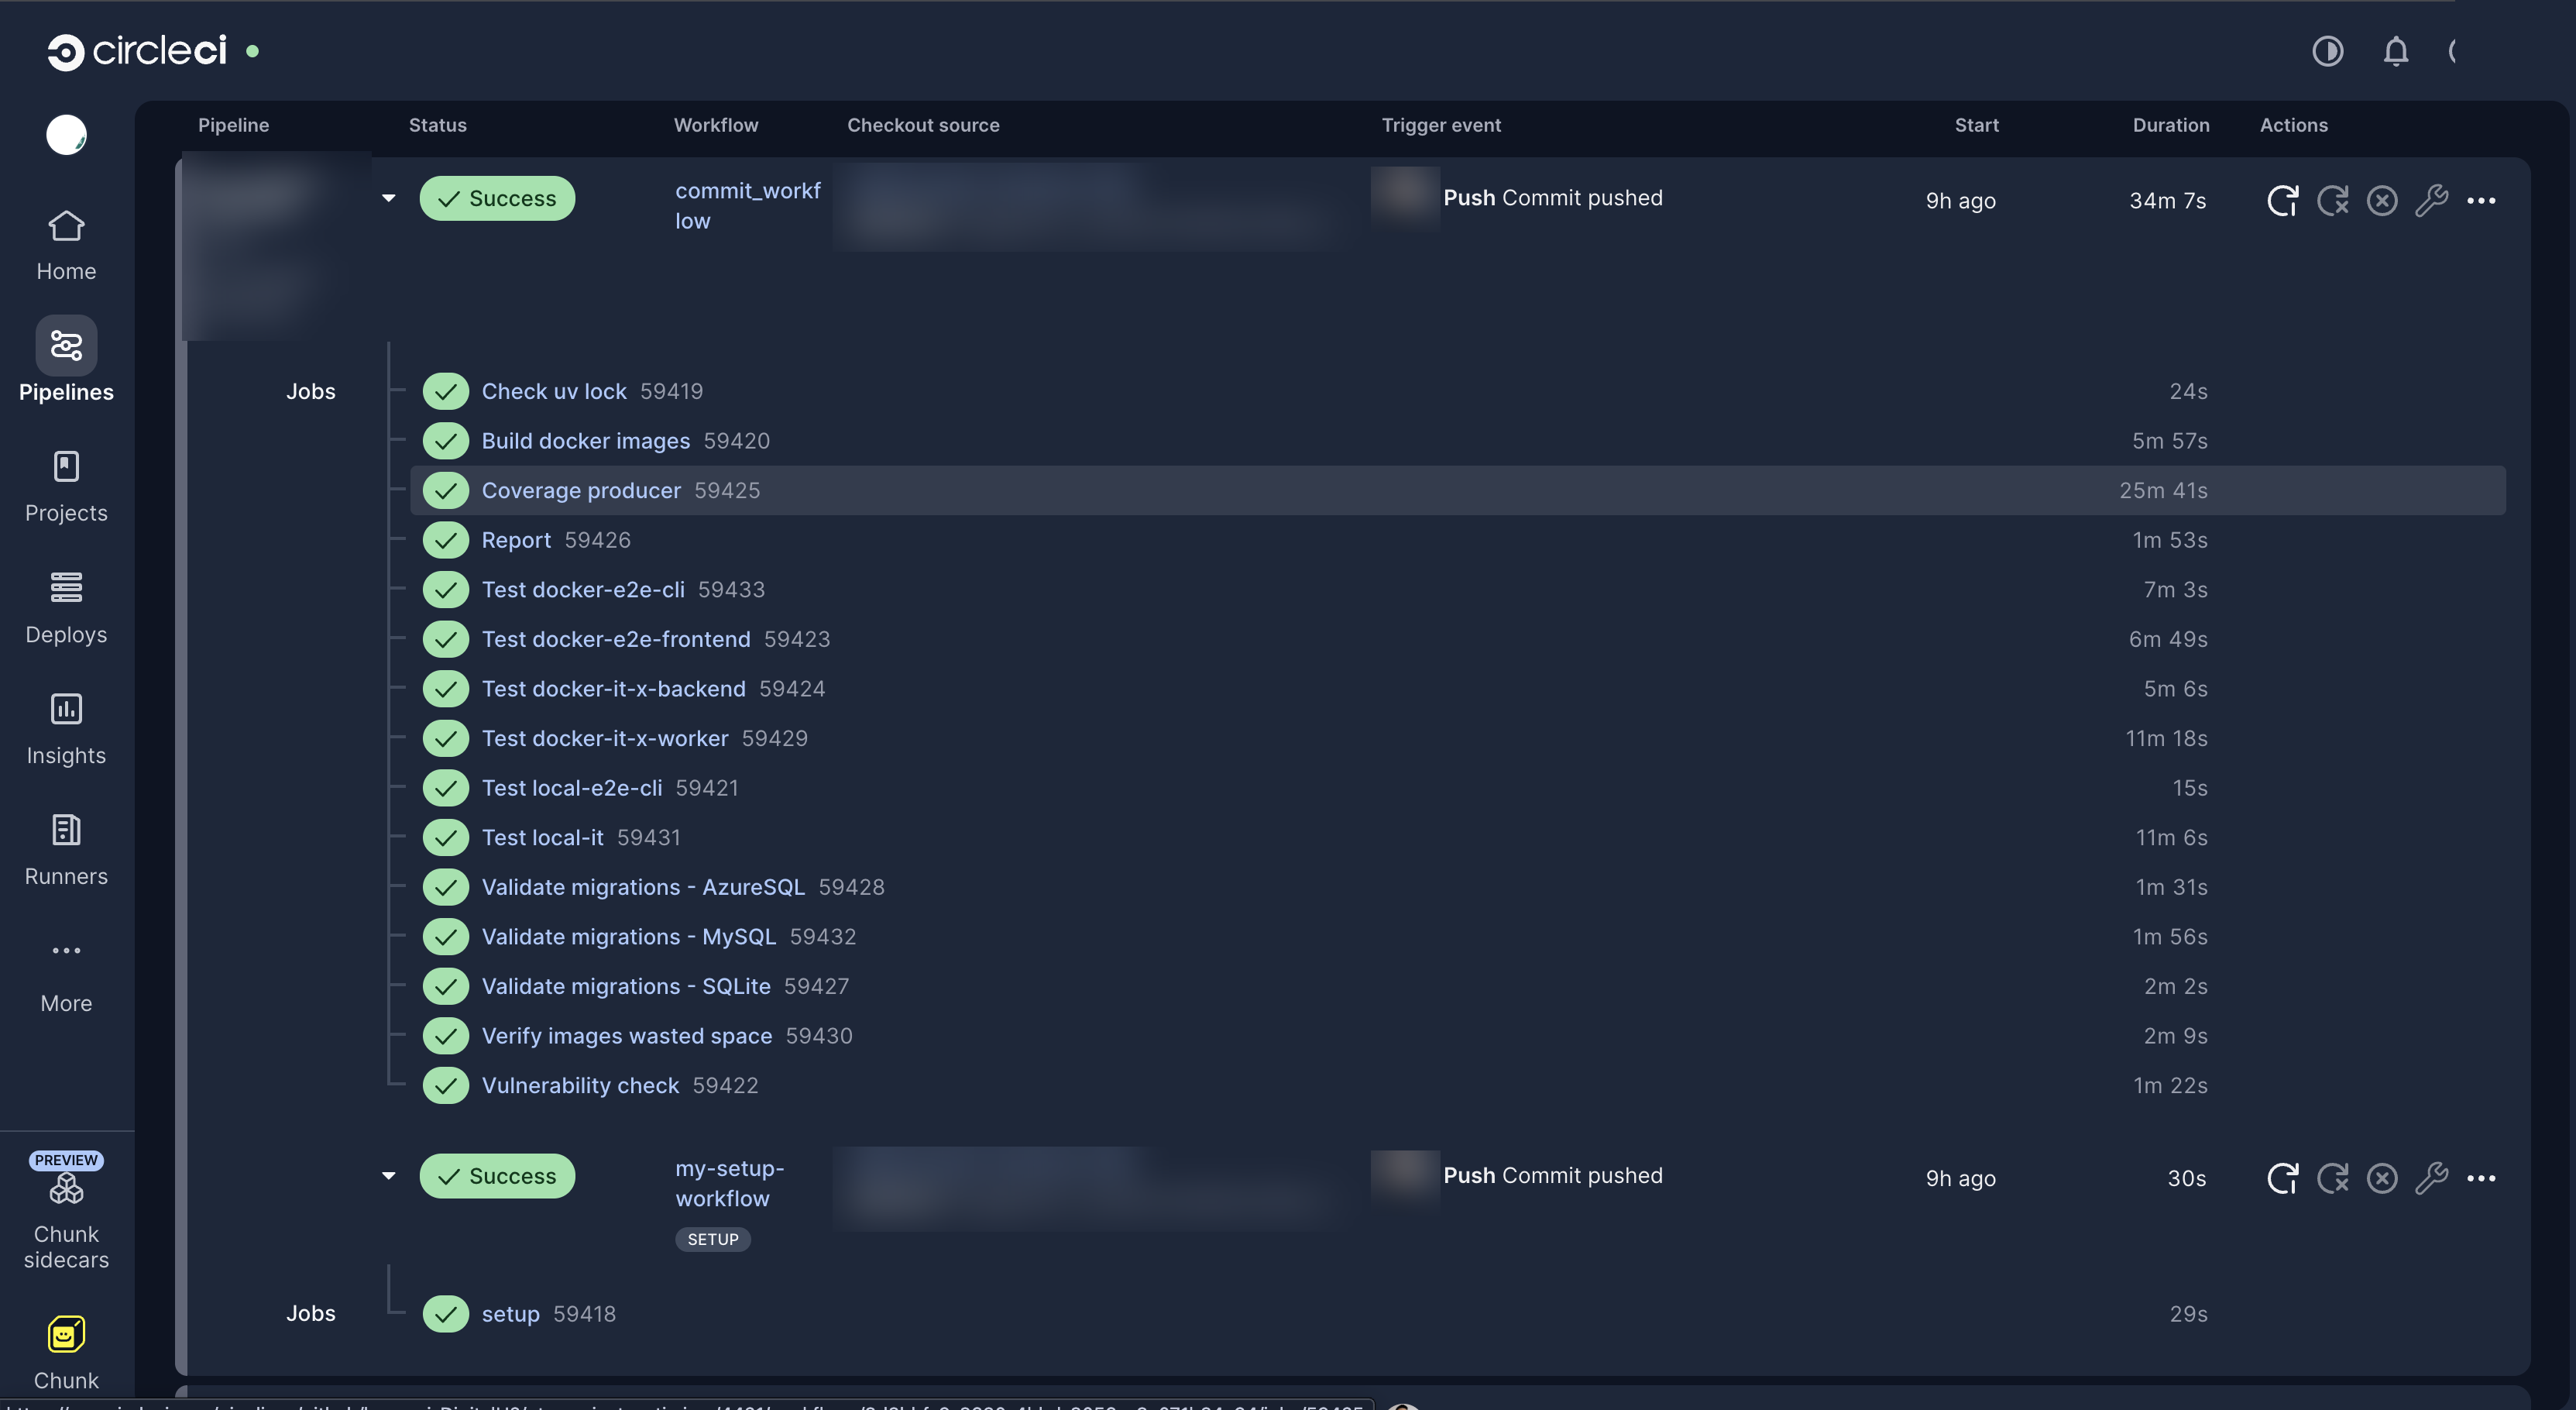
\includegraphics[width=0.95\linewidth]{Figures/chadi_circleci.png}
  \caption{CircleCI workflow: dependency checks, image builds, tests, migrations, and scans.}
  \label{fig:impl-circleci}
\end{figure}

\begin{figure}[H]
  \centering
  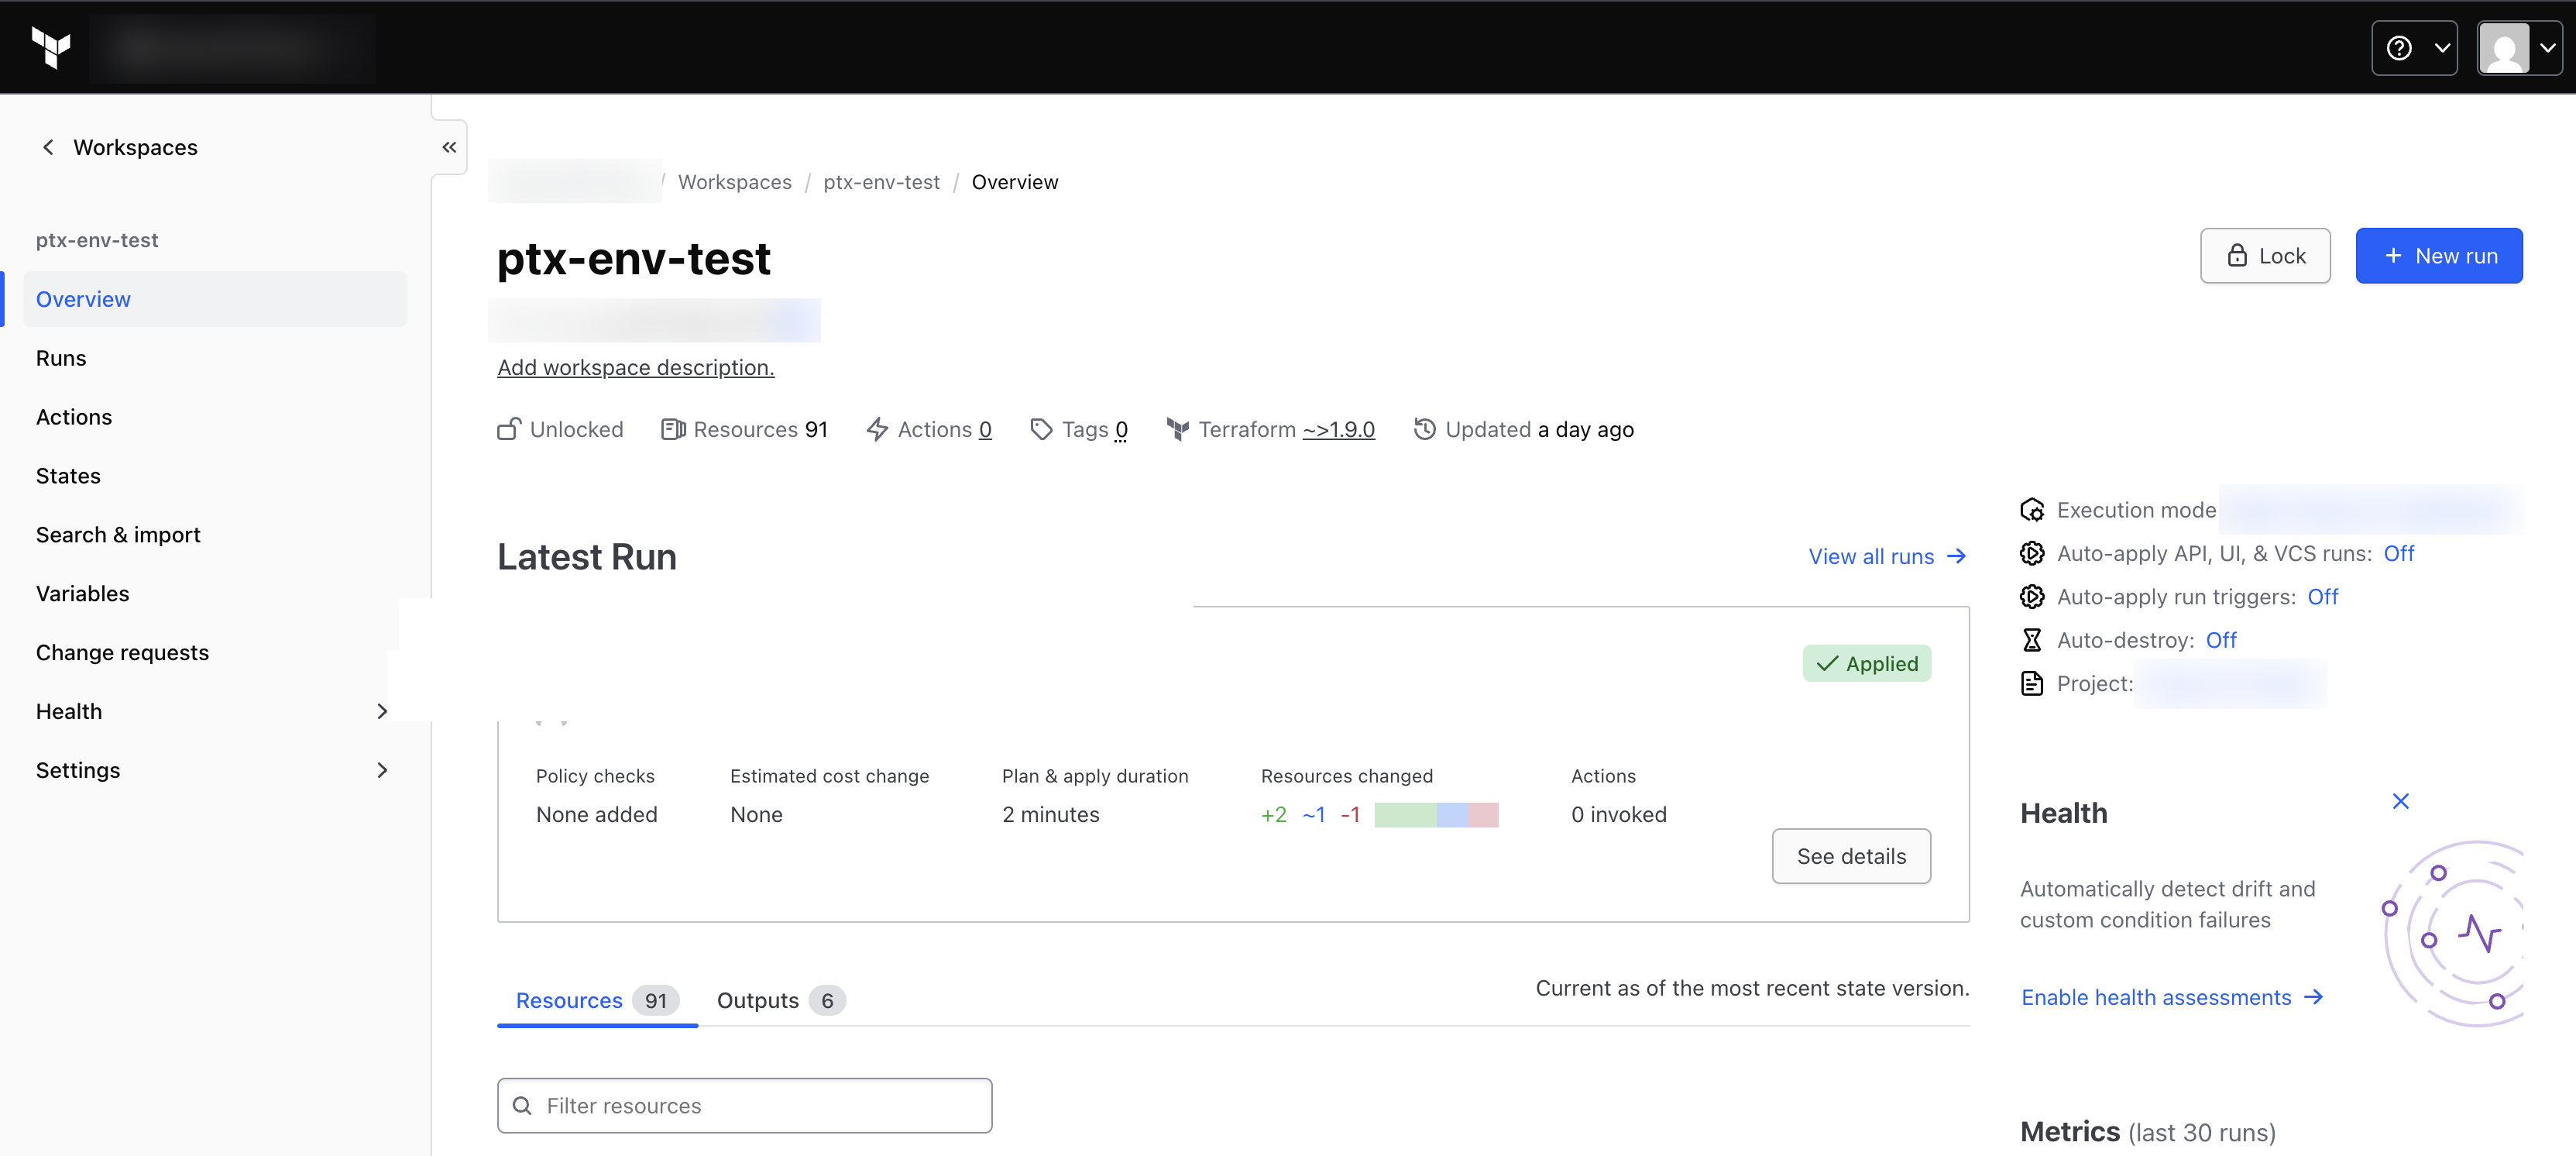
\includegraphics[width=0.95\linewidth]{Figures/chadi_terraform.png}
  \caption{Terraform run: infrastructure applied through a controlled workspace.}
  \label{fig:impl-terraform}
\end{figure}

\subsection{Operational QA and monitoring}

A scheduled monitoring loop assesses the health of the deployed system. It runs
deterministic checks first (public and internal reachability, read-only API checks,
and a synthetic end-to-end journey in a temporary test project) and then asks a
read-only assessment agent for an evidence-based status, summarized as GREEN,
YELLOW, or RED with suspected causes (Figure~\ref{fig:impl-qa}). The write actions
the loop needs (synthetic test setup and cleanup, report persistence, and
notifications) belong to the runner, not to the agent, which preserves the agent's
read-only contract while still surfacing severe findings.

\begin{figure}[H]
  \centering
  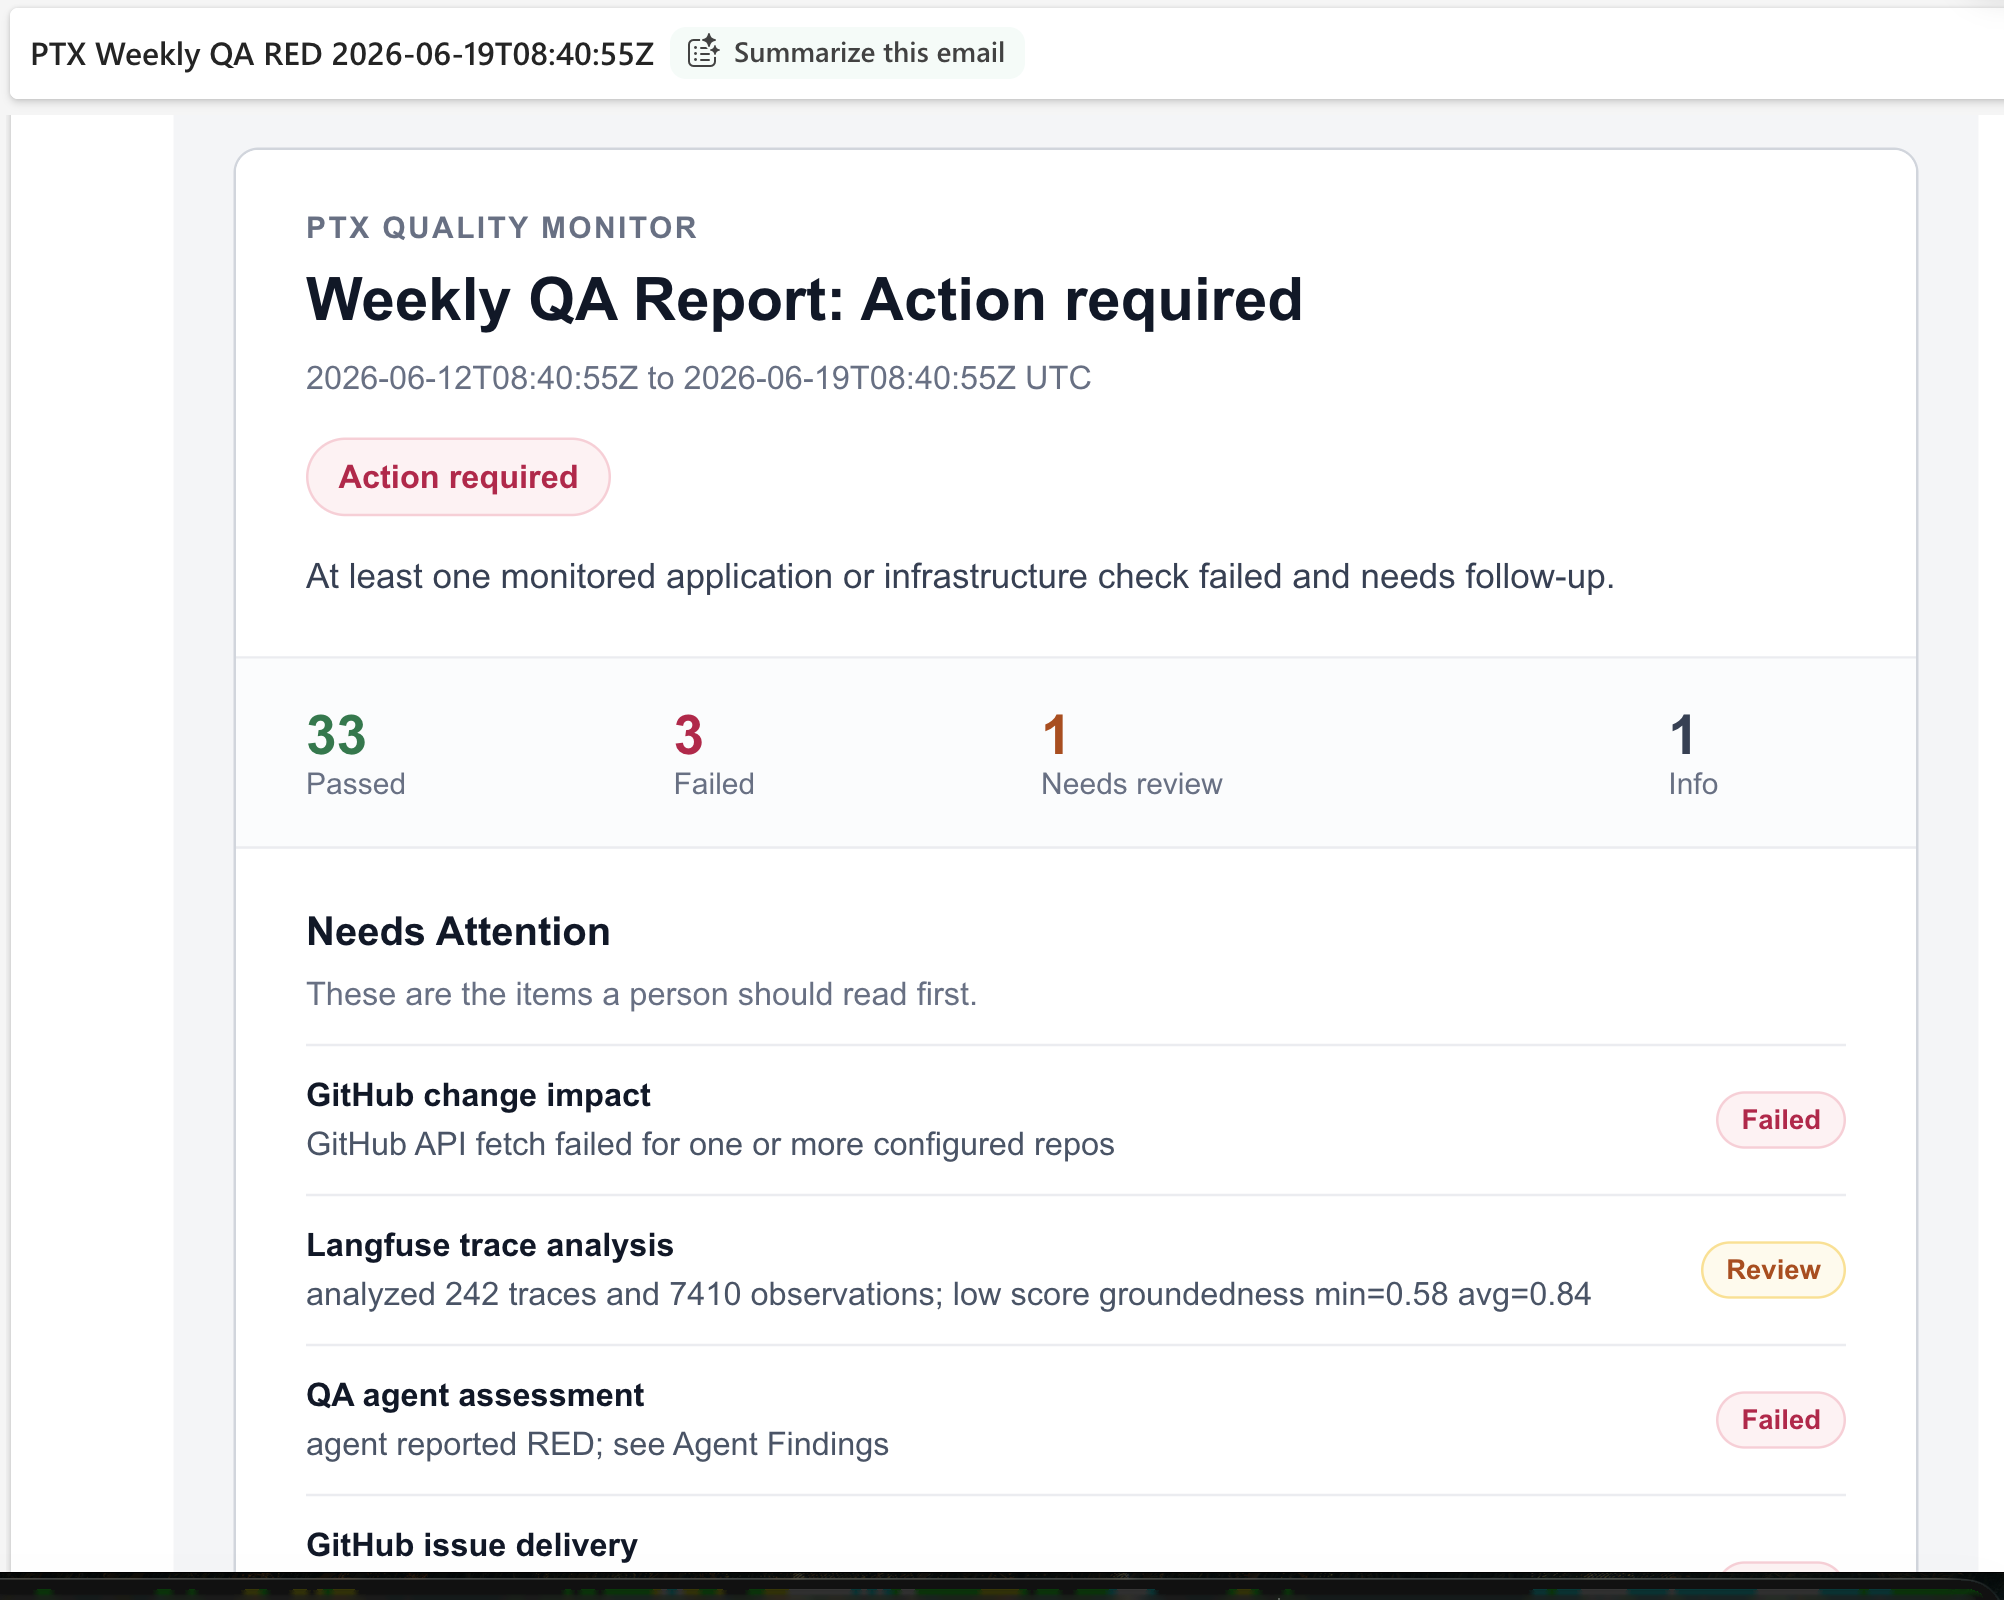
\includegraphics[width=0.62\linewidth]{Figures/chadi_qa_report.png}
  \caption{QA/SRE report: the weekly monitoring summary with items needing attention.}
  \label{fig:impl-qa}
\end{figure}

\subsection{Observability}

Assisted interactions are traced end-to-end in the observability platform, where
model calls, tool invocations, costs, evaluator scores, and prompt versions are
inspectable (Figures~\ref{fig:impl-langfuse} and~\ref{fig:impl-prompts}). This is
the evidence layer that lets a visible answer be traced back to the exact reasoning
and facts that produced it, and the same platform hosts the datasets and experiments
used by the evaluation harness.

\begin{figure}[H]
  \centering
  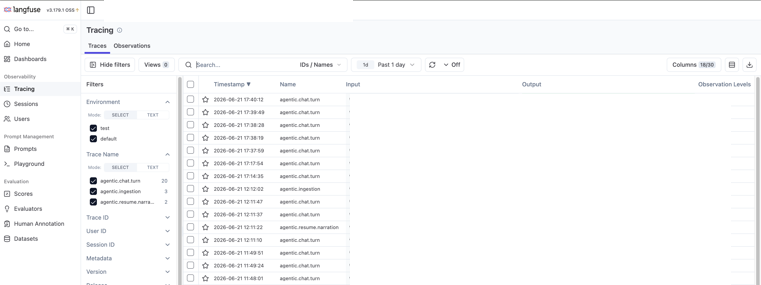
\includegraphics[width=\linewidth]{Figures/impl_langfuse.png}
  \caption{Langfuse traces: each assisted turn with its inputs, outputs, and levels.}
  \label{fig:impl-langfuse}
\end{figure}

\begin{figure}[H]
  \centering
  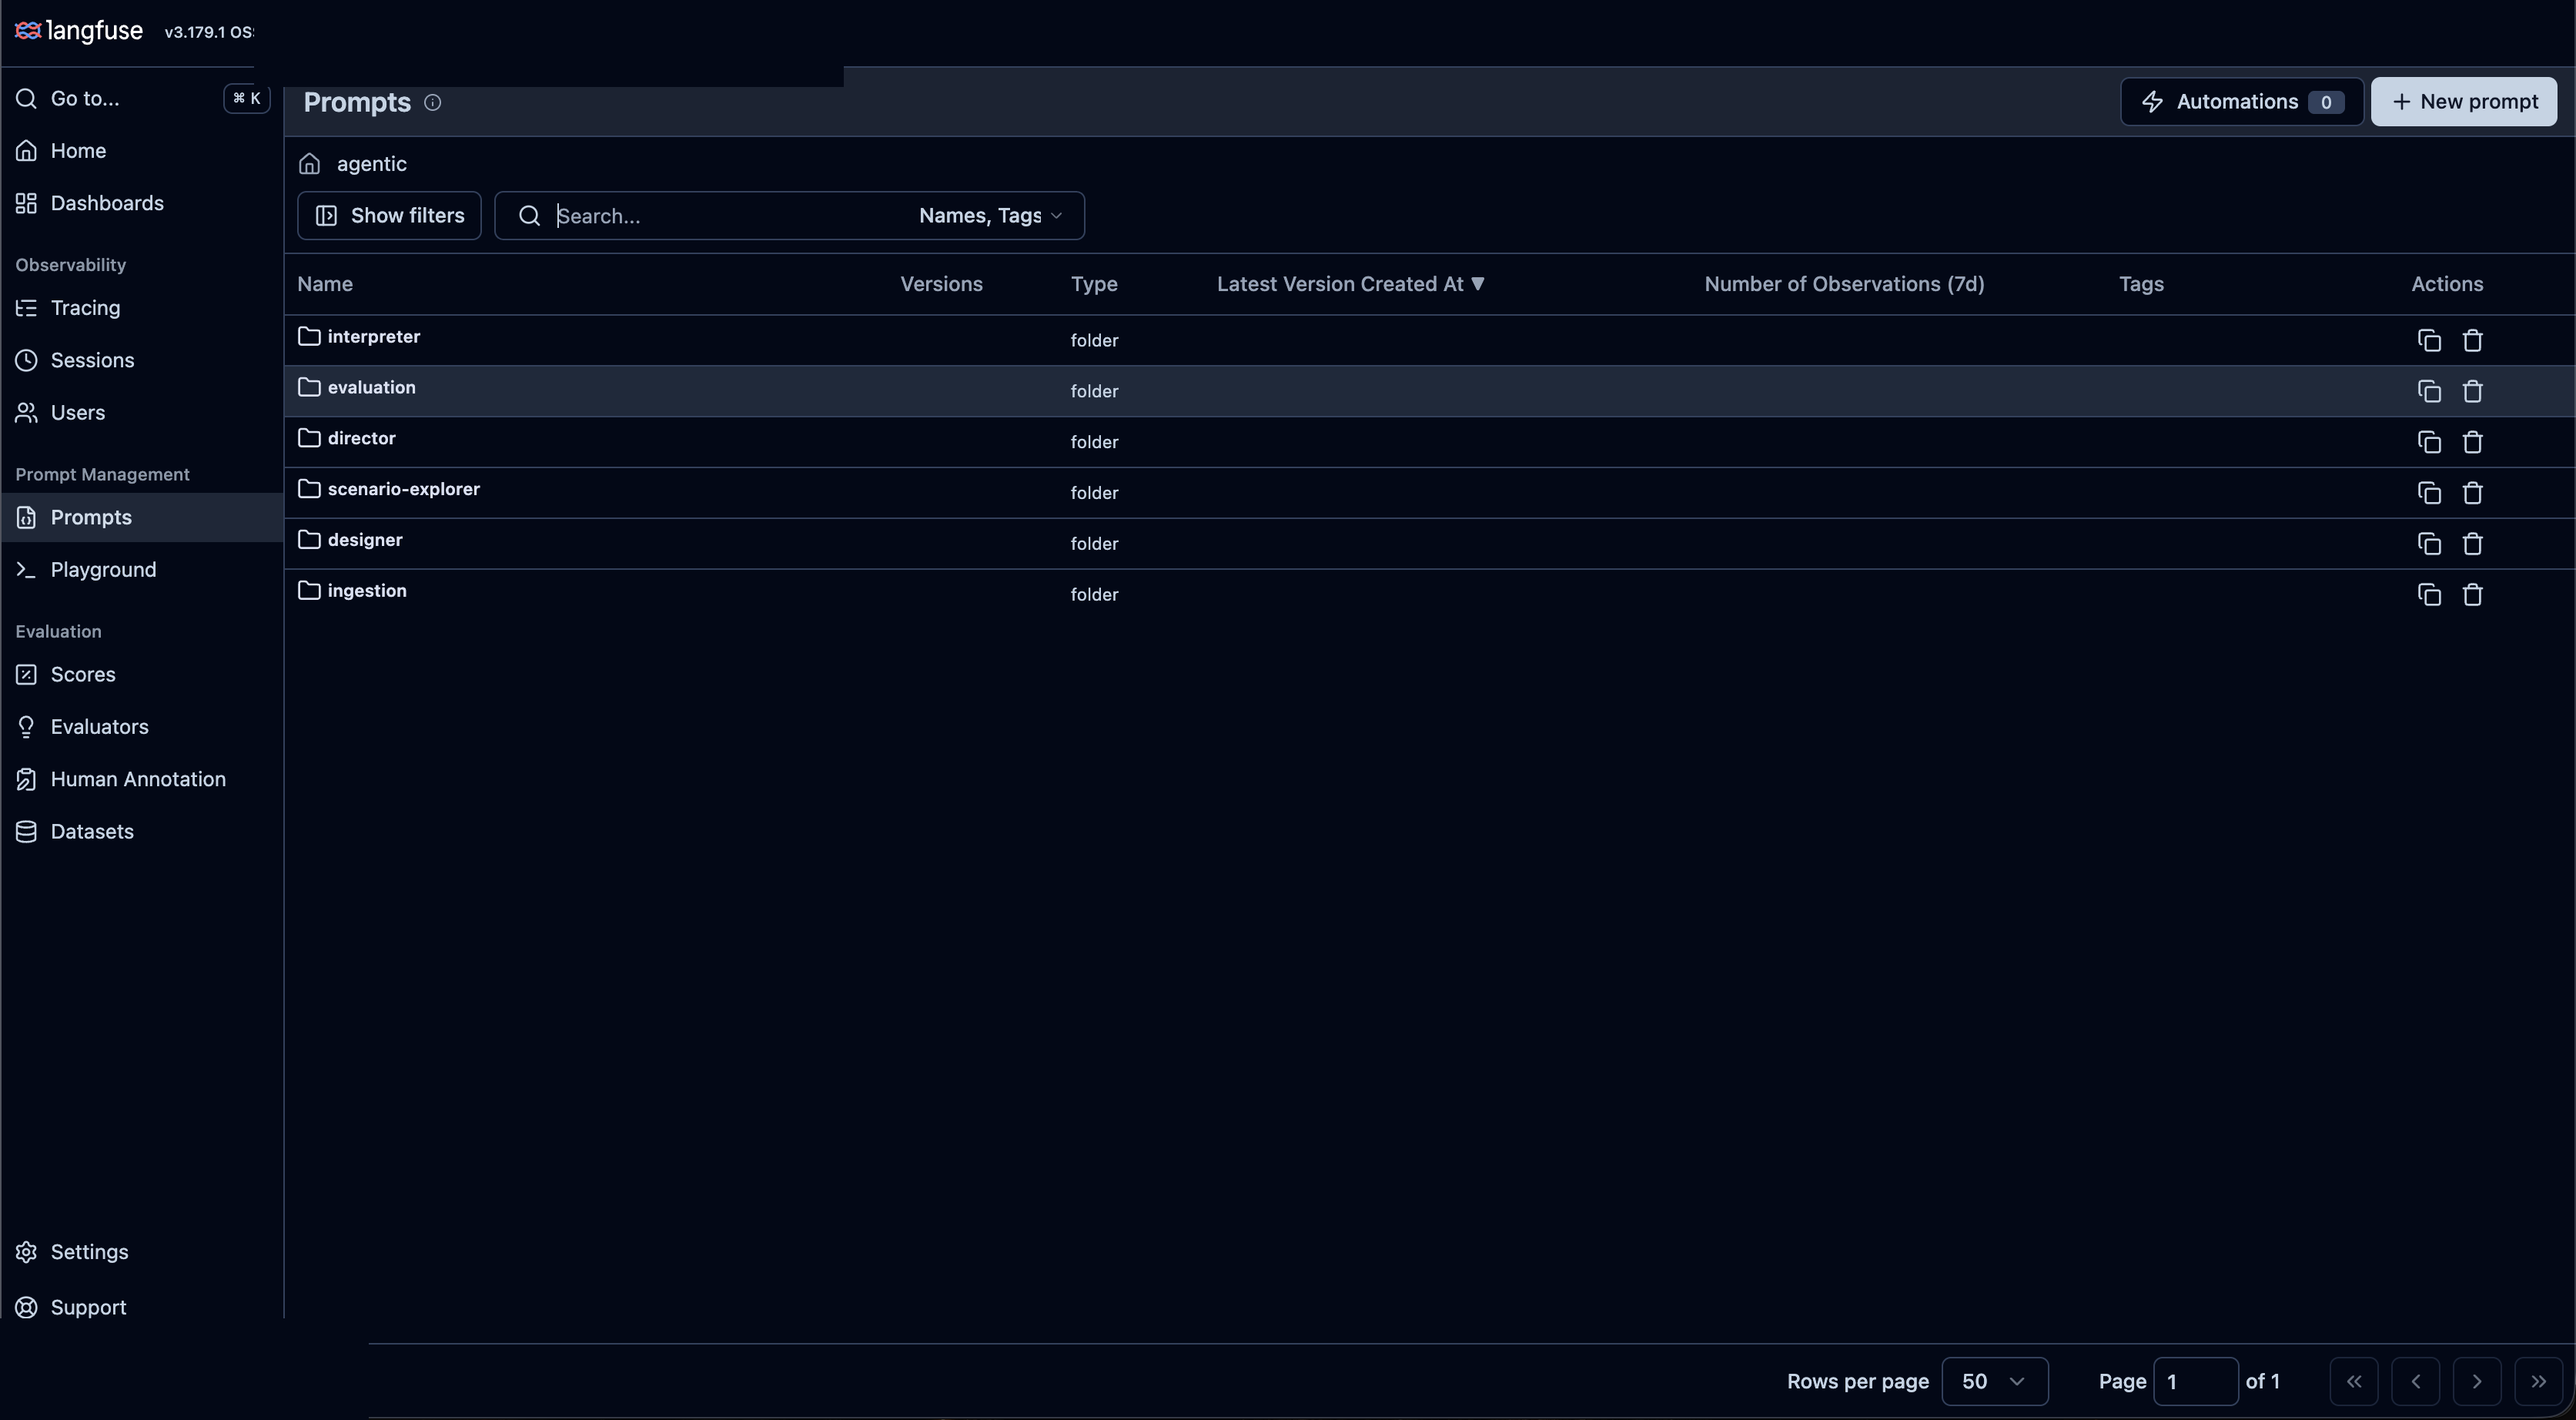
\includegraphics[width=0.9\linewidth]{Figures/chadi_prompt_registry.png}
  \caption{Prompt registry: versioned prompts for the Director and specialist agents.}
  \label{fig:impl-prompts}
\end{figure}

\section{Evaluation}
\label{sec:evaluation}

Because the assisted capabilities rely on a language model, they were measured
rather than assumed. Three complementary measurements are reported: the fidelity of
generated structures tracked across versions, the quality of the interpreter's
explanations scored by an independent judge, and the effort saved per stage of a
study. All are first-order results on a small sample, not a controlled study, and
the absolute figures should be read as order-of-magnitude evidence.\footnote{The
evaluation figures below are drawn from the project's own measurements and should
be confirmed against the final production runs.}

\subsection{Fidelity tracking and regression detection}

For structured outputs such as a generated topology, quality is measured against
curated golden references using a similarity derived from the graph edit distance
\cite{sanfeliu1983}, aggregated over a fixed golden set and compared against an
agreed acceptance threshold. Tracking this metric across versions turns evaluation
into a quantitative, repeatable signal. Figure~\ref{fig:ged} shows the value of the
harness: a change of the underlying model at version~4 silently degraded fidelity
below threshold, a regression that string- or eyeball-level checks would have
missed and that the metric caught before release, prompting a rollback at
version~5.

\begin{figure}[H]
  \centering
  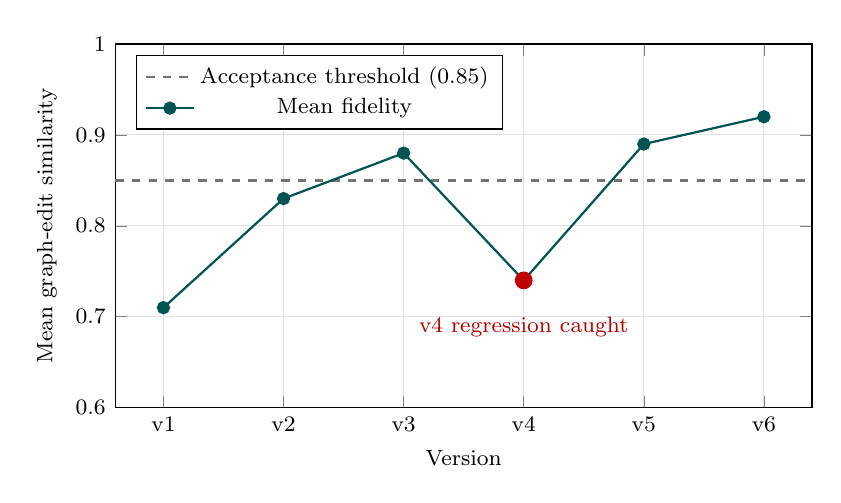
\begin{tikzpicture}
    \begin{axis}[
      width=0.86\linewidth, height=6.2cm,
      xlabel={Version}, ylabel={Mean graph-edit similarity},
      xmin=0.6, xmax=6.4, ymin=0.6, ymax=1.0,
      xtick={1,2,3,4,5,6}, xticklabels={v1,v2,v3,v4,v5,v6},
      ytick={0.6,0.7,0.8,0.9,1.0},
      grid=major, grid style={black!12},
      tick label style={font=\footnotesize}, label style={font=\footnotesize},
      legend style={font=\footnotesize, at={(0.03,0.97)}, anchor=north west},
      clip=false,
    ]
      \addplot[dashed, thick, black!55, samples=2, domain=0.6:6.4] {0.85};
      \addlegendentry{Acceptance threshold (0.85)}
      \addplot[mark=*, thick, teal!65!black] coordinates
        {(1,0.71) (2,0.83) (3,0.88) (4,0.74) (5,0.89) (6,0.92)};
      \addlegendentry{Mean fidelity}
      \addplot[only marks, mark=*, mark size=3pt, red!75!black] coordinates {(4,0.74)};
      \node[font=\footnotesize, red!70!black, anchor=north] at (axis cs:4,0.71)
        {v4 regression caught};
    \end{axis}
  \end{tikzpicture}
  \caption{Topology-designer fidelity across versions; the v4 model swap fell below threshold and was rolled back (illustrative).}
  \label{fig:ged}
\end{figure}

\subsection{Interpretation quality}

Interpretations, which are free text, are scored by an independent LLM-as-a-judge
on the four-dimension rubric of Section~\ref{sec:eval-design} (groundedness,
financial and commercial soundness, and operational coherence), each case scored
several times and aggregated \cite{zheng2023judge}. In the delivered system the same
judge runs in two modes. \textbf{Online}, it fires in the background after each
interpretation, sampled to control cost, and writes its four scores onto that turn's
trace, so quality is visible live (Figure~\ref{fig:impl-judge-scores}).
\textbf{Offline}, it runs over a curated dataset, so a change to the interpreter's
prompt is validated by comparing score deltas across versions as experiments in the
observability platform \cite{langfuse2025}. User thumbs feedback is recorded as
scores and promotes weak turns into the dataset, which closes the loop between
production use and the next round of prompt work. The evaluation is therefore
reproducible on a fixed dataset and tied to explicit dimensions, so a change in
interpretation quality surfaces as a score delta across versions rather than as an
anecdote.

\begin{figure}[H]
  \centering
  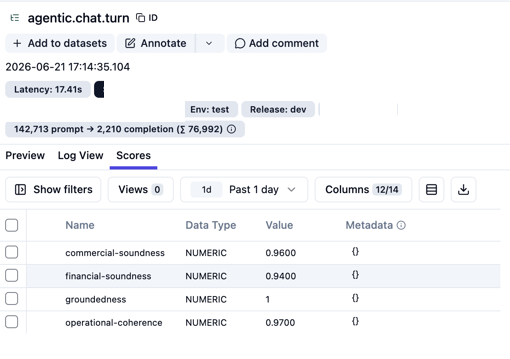
\includegraphics[width=0.72\linewidth]{Figures/impl_judge.png}
  \caption{Automatic evaluation: four judge dimensions on an interpretation's trace (header figures are for the enclosing chat turn).}
  \label{fig:impl-judge-scores}
\end{figure}

\subsection{Impact on analyst effort}

The agentic layer was also assessed against the manual baseline it assists. Each
stage of a study was decomposed into its constituent steps, the manual baseline was
taken from the time practitioners spend today, and the assisted figure was measured
end-to-end with the expert kept in the loop. Figure~\ref{fig:effort} contrasts the
two. The headline for this contribution is the last group: the interpretation of
results, previously a manual expert task, becomes a short grounded conversation.

\begin{figure}[H]
  \centering
  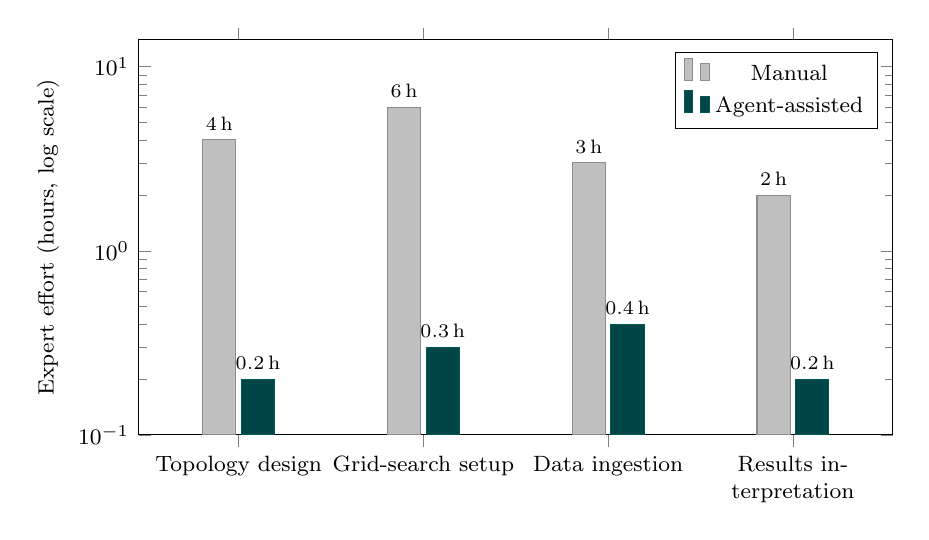
\begin{tikzpicture}
    \begin{axis}[
      ybar, width=0.92\linewidth, height=6.6cm,
      ymode=log, ymin=0.1, ymax=14, log origin=infty,
      ylabel={Expert effort (hours, log scale)},
      symbolic x coords={Topology design, Grid-search setup, Data ingestion,
        Results interpretation},
      xtick=data,
      x tick label style={font=\footnotesize, align=center, text width=2.5cm},
      tick label style={font=\footnotesize}, label style={font=\footnotesize},
      bar width=12pt, enlarge x limits=0.18,
      legend style={font=\footnotesize, at={(0.98,0.97)}, anchor=north east},
      point meta=rawy,
      nodes near coords={\pgfmathprintnumber{\pgfplotspointmeta}\,h},
      every node near coord/.append style={font=\scriptsize, anchor=south},
    ]
      \addplot[fill=black!25, draw=black!45] coordinates
        {(Topology design,4) (Grid-search setup,6) (Data ingestion,3)
         (Results interpretation,2)};
      \addplot[fill=teal!55!black, draw=teal!70!black] coordinates
        {(Topology design,0.2) (Grid-search setup,0.3) (Data ingestion,0.4)
         (Results interpretation,0.2)};
      \legend{Manual, Agent-assisted}
    \end{axis}
  \end{tikzpicture}
  \caption{Expert effort per stage, manual versus agent-assisted (log scale; representative order-of-magnitude estimates).}
  \label{fig:effort}
\end{figure}

Beyond raw time, and arguably more defensible than any single figure, the work
improves \emph{consistency} (every interpretation follows the same grounded
rubric), \emph{traceability} (every figure is linked to a deterministic result),
and \emph{accessibility} (a non-specialist can obtain and audit an interpretation
on the cases evaluated), the qualities that ultimately widen the set of people who
can use the tool.

\section*{Conclusion}

This chapter presented the concrete implementation of the restored and extended
Energy Transition Optimizer. It identified the main technologies across the
frontend, backend, deterministic execution, agentic layer, persistence, cloud
runtime, identity, and delivery; documented the
implemented product through the showcase, from product entry and the deterministic
workspace to agentic creation, ingestion, topology generation, and result
exploration and interpretation; and reported the
platform and operations work around enterprise access, automated delivery,
infrastructure-as-code, QA monitoring, and observability. It closed with the
evaluation: a fidelity metric that catches regressions, an LLM-as-a-judge scoring
of interpretations, and an order-of-magnitude reduction in the effort required to
interpret results. Deterministic computation remains the source of numerical truth,
assisted workflows remain approval-gated, and platform operation is supported by
repeatable deployment and observable runtime behavior. The general conclusion now
summarizes the outcomes of the internship and its broader perspectives.


\chapter*{Industrial Recognition: A Granted Patent}
\addcontentsline{toc}{chapter}{Industrial Recognition: A Granted Patent}
\markboth{Industrial Recognition: A Granted Patent}{Industrial Recognition: A Granted Patent}
\label{chap:patent}

% This chapter is unnumbered, so give its floats their own prefix instead of
% inheriting Chapter 5's counters.
\setcounter{figure}{0}
\renewcommand{\thefigure}{P.\arabic{figure}}
\setcounter{table}{0}
\renewcommand{\thetable}{P.\arabic{table}}

The industrial significance of the platform on which this internship was carried
out was formally recognized while the work was under way. The core Power-to-X
optimization method at the heart of the Energy Transition Optimizer is protected
by a United States patent granted to Boston Consulting Group,
\textbf{US~12,711,433~B2}, \emph{Systems and Techniques for Optimizing the
Implementation and Operation of Power-to-X Plants}, issued on 18~August~2026
\cite{bcgptx2026}. The application was filed in September~2023 and published in
March~2025, so the engine that this report treats as the numerical authority was,
throughout the internship, a patent-pending industrial asset, and its grant
landed as this report was being finalized. Table~\ref{tab:patent} gathers its
bibliographic details, and Figure~\ref{fig:patent-firstpage} reproduces the
patent's front page.

\begin{figure}[H]
  \centering
  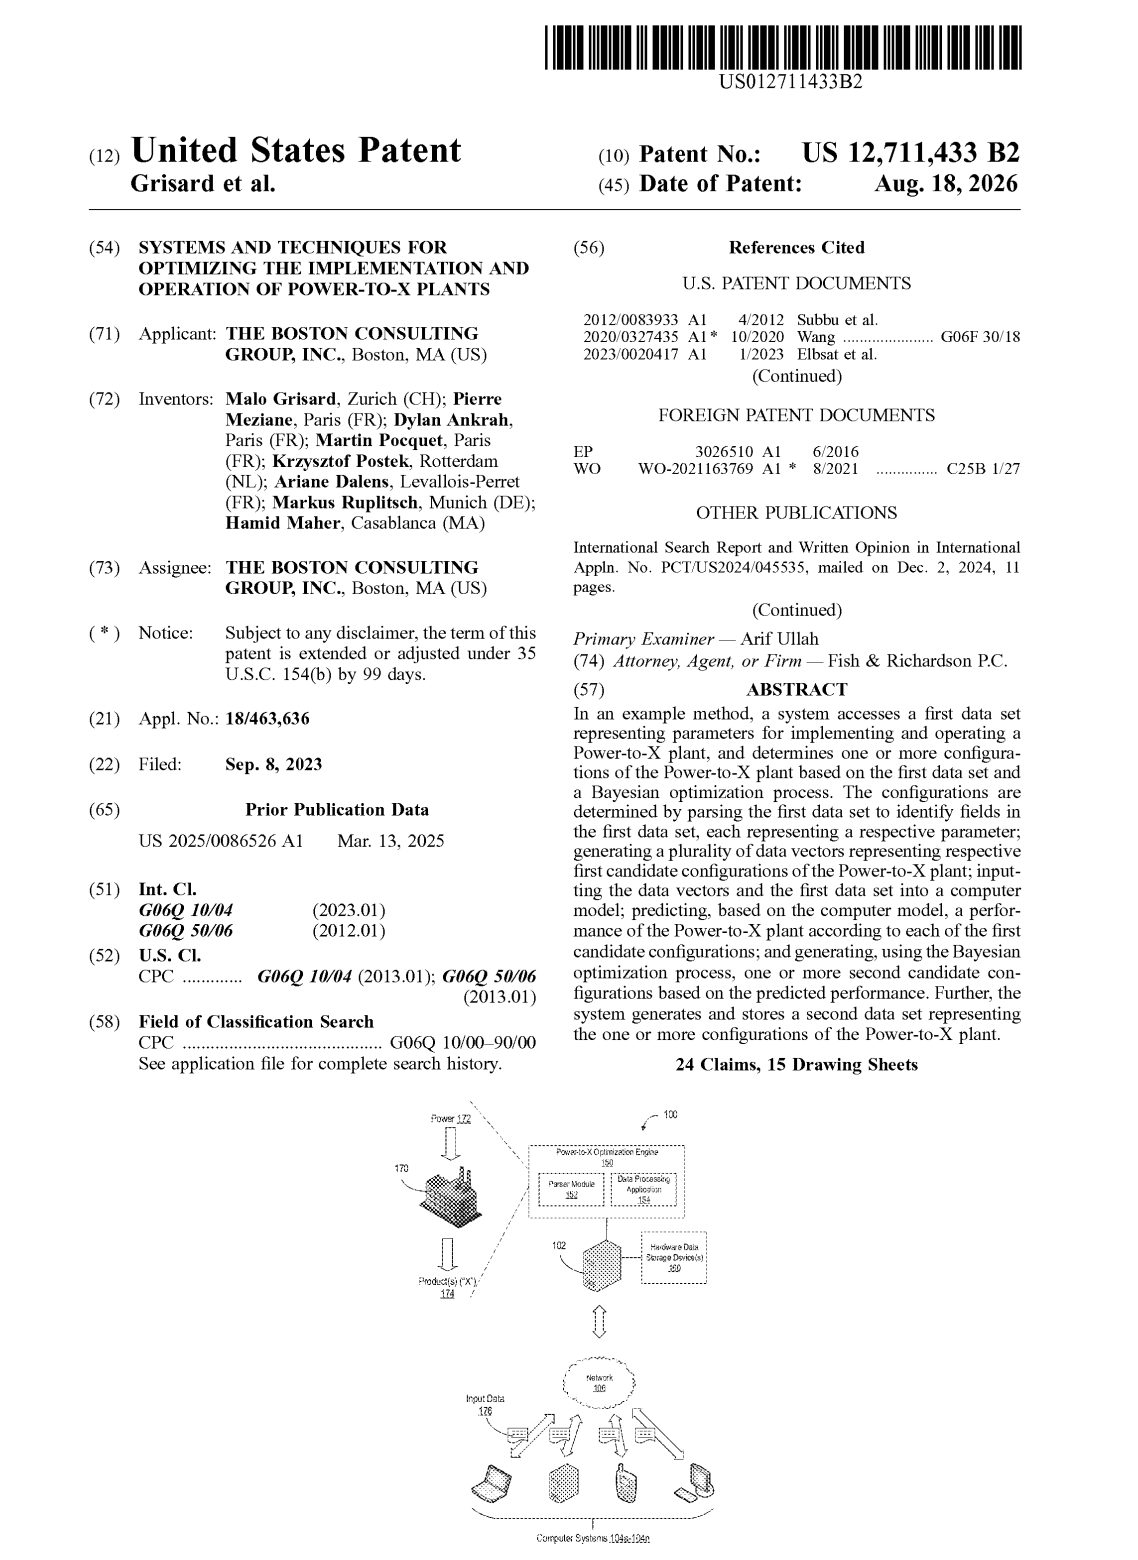
\includegraphics[width=0.8\linewidth]{Figures/patent.png}
  \caption{The granted patent US~12,711,433~B2: cover sheet of the public USPTO
    document.}
  \label{fig:patent-firstpage}
\end{figure}

\begin{table}[H]
  \centering
  \small
  \begin{tabularx}{\linewidth}{@{}>{\raggedright\arraybackslash}p{3.4cm} >{\raggedright\arraybackslash}X@{}}
    \toprule
    \textbf{Field} & \textbf{Detail} \\
    \midrule
    Patent number & US~12,711,433~B2 \\
    \addlinespace
    Title & Systems and Techniques for Optimizing the Implementation and
      Operation of Power-to-X Plants \\
    \addlinespace
    Assignee & The Boston Consulting Group, Inc. (Boston, MA, USA) \\
    \addlinespace
    Inventors & M.~Grisard, P.~Meziane, D.~Ankrah, M.~Pocquet, K.~Postek,
      A.~Dalens, M.~Ruplitsch, and H.~Maher \\
    \addlinespace
    Application & No.~18/463,636, filed 8~September~2023 \\
    \addlinespace
    Prior publication & US~2025/0086526~A1, 13~March~2025 \\
    \addlinespace
    Date of grant & 18~August~2026 \\
    \addlinespace
    Classification & G06Q~10/04; G06Q~50/06 (operations research and energy) \\
    \addlinespace
    Scope & 24~claims, 15~drawing sheets \\
    \bottomrule
  \end{tabularx}
  \caption{Bibliographic details of the granted patent covering the optimizer's
    core method.}
  \label{tab:patent}
\end{table}

\section*{What the patent protects}

The patent covers the optimizer's core method for determining strong plant
configurations. In the terms of its abstract, a system accesses a data set of
parameters for implementing and operating a Power-to-X plant, parses that data
set to identify the fields that represent each parameter, and generates a set of
data vectors that stand for candidate plant configurations. Those candidates and
the parameter set are passed to a computer model that predicts the performance of
the plant under each configuration, and a \textbf{Bayesian optimization} process
then proposes new candidate configurations from the predicted performance,
iterating toward strong designs and storing the resulting configurations.

This is the formal description of the capability that
Chapter~\ref{chap:context} introduced as the deterministic engine and its
parameter search: turning a typed description of a plant and its assumptions into
optimized, evaluated configurations with auditable financial indicators. The two
descriptions operate at different layers, and it is worth being precise about the
distinction. The patent's \textbf{Bayesian optimization} is a strategy for
\emph{choosing} which candidate configurations to evaluate next; each configuration
is then scored by the \textbf{deterministic} simulation that this report treats as
the numerical authority. The product as studied here drives that same deterministic
engine through an exhaustive \textbf{grid search} over the design space rather than
the patented Bayesian search, so the "deterministic engine and its parameter search"
of Chapter~\ref{chap:context} and the patented method share the deterministic
per-configuration evaluation while differing in how the design space is explored.

\section*{Relation to this work}

Two points connect this grant to the present report. First, it concerns the
\textbf{deterministic optimization core, not the governed agentic layer} that is
the subject of this internship. The application predates the internship, and the
author of this report is not among the named inventors; several members of the
team he worked with are, including the product's technical lead. The patent
therefore belongs to the surrounding product context established in
Chapter~\ref{chap:context}, not to the work detailed in
Chapters~\ref{chap:design} and~\ref{chap:implementation}. A granted patent
certifies novelty and industrial applicability in the legal sense; it is presented
here as industrial context, not as evidence of the system's performance or adoption,
which are the province of the evaluation in Chapter~\ref{chap:implementation}.

Second, and more importantly, the grant sharpens the central principle defended
throughout this report. The patented method is precisely the \emph{numerical
authority} that the agentic layer is designed to serve rather than replace: the
assistant prepares inputs, explains outputs, and guides the workflow, while the
protected optimization engine remains the sole source of the configurations and
the financial indicators. Building a governed, grounded assistance layer on top of
a patented core is exactly the product-level investment described in
Section~\ref{sec:internal-product}. It lowers the barrier to using a valuable,
protected capability for every future client adaptation, without diluting the
reproducibility and auditability that make that capability worth protecting. From
an industrial-property standpoint, the grant reinforces the same separation between
assistance and authority that this report upholds from an engineering one.


\chapter*{General Conclusion and Perspectives}
\addcontentsline{toc}{chapter}{General Conclusion and Perspectives}
\markboth{General Conclusion and Perspectives}{General Conclusion and Perspectives}

This report addressed a question raised by the modernization of the Energy
Transition Optimizer, an internal BCG~X product for the pre-feasibility analysis
of Power-to-X projects: how can generative AI make an expert-only techno-economic
optimizer accessible in natural language, without compromising the
reproducibility, auditability, and human control its results demand? The answer
defended throughout is a separation between assistance and authority: the
deterministic engine remains the sole source of numerical truth, while a governed
multi-agent layer helps users design, run, and understand a study, with every
state-changing action validated and explicitly approved before it takes effect.

The four scoping questions of Chapter~\ref{chap:context} can now be answered
directly. \emph{What can be delegated:} language models proved well suited to
preparing inputs and explaining outputs, topology drafting, assumption ingestion,
scenario framing, and result interpretation, while every numerical result stayed
with the deterministic engine. \emph{How assisted actions are made trustworthy:}
each state change is a typed, validated proposal that a human approves, and each
assisted turn is traced, so actions are auditable and, taking effect only on
approval, reversible by rejection. \emph{How a non-deterministic capability is
measured:} an independent LLM-as-a-judge scores interpretations on four explicit
dimensions, and a graph-edit-distance metric scores generated structures, both
tracked across versions rather than assumed. \emph{How the work stays adaptable
across clients:} the layer was built as a reusable product capability on a
reproducible, infrastructure-as-code platform, so the same core is adapted per
client rather than rebuilt.

Conducted as a team, the project delivered this on two fronts. It restored the
platform foundation, with federated enterprise identity, reproducible delivery,
and operational observability. And it introduced the governed multi-agent layer
itself, a Director that routes each request to specialist agents for ingestion,
topology design, scenario exploration, and interpretation, behind typed proposals
and human approval. The industrial value of the core this layer serves was
independently confirmed while the work was under way, when the optimizer's
optimization method was granted a United States patent, presented in the
preceding chapter.

At the heart of that layer stand three pillars: a
\textbf{read-only interpretation agent} that explains a simulation population in
plain language while keeping every figure traceable to a deterministic result; a
\textbf{visualization layer}, with interactive scatter exploration and a navigable
discounted-cash-flow table, that makes results legible and carries the
interpretation on demand; and an \textbf{evaluation harness} that measures the
grounding and soundness of interpretations, with a graph-edit-distance metric for
structured outputs. Together they let a non-specialist obtain and audit an
interpretation that previously required an expert. On the small, first-order sample
we evaluated, each assisted stage of a study fell by roughly an order of magnitude
in expert effort, with result interpretation dropping from about two hours to about
twelve minutes (Chapter~\ref{chap:implementation}); these figures are indicative
rather than controlled, and a study with non-specialist participants remains future
work.

The main lesson is that trust in an assisted analytical tool cannot rest on
prompting alone: it depends on the architecture (the read/write split, the approval
gates, the grounding rules), on evidence (measuring the assistant rather than
assuming it), on operations (end-to-end tracing and observability), and ultimately
on the human who approves each state change. Safety, on this view, is a property of
that whole arrangement, and one demonstrated on the analyses we ran rather than
proven in general. Natural extensions follow the same logic: richer comparative
interpretation, broader and human-calibrated evaluation coverage, adversarial
testing of the governance boundaries, and adaptation of these capabilities to each
new client deployment.

On a personal level, the internship strengthened my skills in AI orchestration,
in language-model evaluation and observability, in data visualization, and in
techno-economic financial literacy. Above all, it taught me the discipline it
takes for generative AI to earn trust in a tool whose value depends on being
right, and that is the standard I intend to carry into what I build next.


\appendix


%\input{Endmatter/Glossary}

%\input{Endmatter/Acronyms}

%\input{Endmatter/ComplementaryCodes}

\begin{thebibliography}{99}
\addcontentsline{toc}{chapter}{Bibliography}

%% --- Optimization and operations research ---

\bibitem{bertsimas1997}
D.~Bertsimas and J.~N. Tsitsiklis.
\emph{Introduction to Linear Optimization}.
Athena Scientific, Belmont, MA, 1997.

\bibitem{nemhauser1988}
G.~L. Nemhauser and L.~A. Wolsey.
\emph{Integer and Combinatorial Optimization}.
Wiley-Interscience, 1988.

\bibitem{morales2013}
G.~Morales-Espa\~{n}a, J.~M. Latorre, and A.~Ramos.
Tight and compact MILP formulation for the thermal unit commitment problem.
\emph{IEEE Transactions on Power Systems}, 28(4):4897--4908, 2013.

\bibitem{wood2013}
A.~J. Wood, B.~F. Wollenberg, and G.~B. Shebl\'{e}.
\emph{Power Generation, Operation, and Control}.
Wiley, 3rd edition, 2013.

%% --- Energy-system and Power-to-X modelling ---

\bibitem{geidl2007opf}
M.~Geidl and G.~Andersson.
Optimal power flow of multiple energy carriers.
\emph{IEEE Transactions on Power Systems}, 22(1):145--155, 2007.

\bibitem{geidl2007hub}
M.~Geidl, G.~Koeppel, P.~Favre-Perrod, B.~Kl\"{o}ckl, G.~Andersson, and
K.~Fr\"{o}hlich.
Energy hubs for the future.
\emph{IEEE Power and Energy Magazine}, 5(1):24--30, 2007.

\bibitem{ueckerdt2021}
F.~Ueckerdt, C.~Bauer, A.~Dirnaichner, J.~Everall, R.~Sacchi, and G.~Luderer.
Potential and risks of hydrogen-based e-fuels in climate change mitigation.
\emph{Nature Climate Change}, 11:384--393, 2021.

\bibitem{hermesmann2021}
M.~Hermesmann, K.~Gr\"{u}bel, L.~Scherotzki, and T.~E. M\"{u}ller.
Promising pathways: the geographic and energetic potential of Power-to-X
technologies based on regeneratively obtained hydrogen.
\emph{Renewable and Sustainable Energy Reviews}, 138:110644, 2021.

\bibitem{oemof2018}
S.~Hilpert, C.~Kaldemeyer, U.~Krien, S.~G\"{u}nther, C.~Wingenbach, and
G.~Ple\ss{}mann.
The open energy modelling framework (oemof).
\emph{Energy Strategy Reviews}, 22:16--25, 2018.

\bibitem{pfenninger2018}
S.~Pfenninger et al.
Opening the black box of energy modelling: strategies and lessons learned.
\emph{Energy Strategy Reviews}, 19:63--71, 2018.

\bibitem{aace2020}
AACE International.
\emph{Cost Estimate Classification System as Applied in Engineering,
Procurement, and Construction for the Process Industries}.
Recommended Practice 18R-97, rev. 2020.

\bibitem{irena2023}
International Renewable Energy Agency (IRENA).
\emph{Renewable Power Generation Costs in 2023}.
IRENA, 2024.

%% --- Solvers ---

\bibitem{ortools}
L.~Perron and V.~Furnon.
\emph{OR-Tools}.
Google, \href{https://developers.google.com/optimization}{developers.google.com/optimization}.

\bibitem{highs2018}
Q.~Huangfu and J.~A.~J. Hall.
Parallelizing the dual revised simplex method.
\emph{Mathematical Programming Computation}, 10(1):119--142, 2018.

\bibitem{gurobi2024}
Gurobi Optimization, LLC.
\emph{Gurobi Optimizer Reference Manual}, 2024.

%% --- Large language models, agents, and tool use ---

\bibitem{vaswani2017}
A.~Vaswani, N.~Shazeer, N.~Parmar, J.~Uszkoreit, L.~Jones, A.~N. Gomez,
{\L}.~Kaiser, and I.~Polosukhin.
Attention is all you need.
In \emph{Advances in Neural Information Processing Systems (NeurIPS)}, 2017.

\bibitem{wei2022cot}
J.~Wei, X.~Wang, D.~Schuurmans, M.~Bosma, B.~Ichter, F.~Xia, E.~Chi, Q.~Le, and
D.~Zhou.
Chain-of-thought prompting elicits reasoning in large language models.
In \emph{Advances in Neural Information Processing Systems (NeurIPS)}, 2022.

\bibitem{yao2023react}
S.~Yao, J.~Zhao, D.~Yu, N.~Du, I.~Shafran, K.~Narasimhan, and Y.~Cao.
ReAct: synergizing reasoning and acting in language models.
In \emph{International Conference on Learning Representations (ICLR)}, 2023.

\bibitem{schick2023toolformer}
T.~Schick, J.~Dwivedi-Yu, R.~Dess\`{i}, R.~Raileanu, M.~Lomeli, L.~Zettlemoyer,
N.~Cancedda, and T.~Scialom.
Toolformer: language models can teach themselves to use tools.
In \emph{Advances in Neural Information Processing Systems (NeurIPS)}, 2023.

\bibitem{wu2024autogen}
Q.~Wu, G.~Bansal, J.~Zhang, Y.~Wu, B.~Li, E.~Zhu, L.~Jiang, X.~Zhang, S.~Zhang,
J.~Liu, A.~H. Awadallah, R.~W. White, D.~Burger, and C.~Wang.
AutoGen: enabling next-gen LLM applications via multi-agent conversation.
In \emph{Conference on Language Modeling (COLM)}, 2024.

\bibitem{wang2024survey}
L.~Wang et al.
A survey on large language model based autonomous agents.
\emph{Frontiers of Computer Science}, 18(6), 2024.

\bibitem{lewis2020rag}
P.~Lewis, E.~Perez, A.~Piktus, F.~Petroni, V.~Karpukhin, N.~Goyal,
H.~K\"{u}ttler, M.~Lewis, W.-t. Yih, T.~Rockt\"{a}schel, S.~Riedel, and
D.~Kiela.
Retrieval-augmented generation for knowledge-intensive NLP tasks.
In \emph{Advances in Neural Information Processing Systems (NeurIPS)}, 2020.

\bibitem{mcp2024}
Anthropic.
\emph{Model Context Protocol (MCP) Specification}.
\href{https://modelcontextprotocol.io}{modelcontextprotocol.io}, 2024.

\bibitem{langgraph2024}
LangChain.
\emph{LangGraph: building stateful, multi-actor applications with LLMs}.
\href{https://langchain-ai.github.io/langgraph/}{langchain-ai.github.io/langgraph}, 2024.

%% --- Trust, evaluation, and observability ---

\bibitem{greshake2023}
K.~Greshake, S.~Abdelnabi, S.~Mishra, C.~Endres, T.~Holz, and M.~Fritz.
Not what you've signed up for: compromising real-world LLM-integrated
applications with indirect prompt injection.
In \emph{ACM Workshop on Artificial Intelligence and Security (AISec)}, 2023.

\bibitem{zheng2023judge}
L.~Zheng, W.-L. Chiang, Y.~Sheng, S.~Zhuang, Z.~Wu, Y.~Zhuang, Z.~Lin, Z.~Li,
D.~Li, E.~P. Xing, H.~Zhang, J.~E. Gonzalez, and I.~Stoica.
Judging LLM-as-a-judge with MT-Bench and Chatbot Arena.
In \emph{Advances in Neural Information Processing Systems (NeurIPS)}, 2023.

\bibitem{sanfeliu1983}
A.~Sanfeliu and K.-S. Fu.
A distance measure between attributed relational graphs for pattern recognition.
\emph{IEEE Transactions on Systems, Man, and Cybernetics}, SMC-13(3):353--362,
1983.

\bibitem{langfuse2025}
Langfuse.
\emph{Langfuse: open-source LLM engineering platform}.
\href{https://langfuse.com}{langfuse.com}, 2025.

%% --- Patent ---

\bibitem{bcgptx2026}
M.~Grisard, P.~Meziane, D.~Ankrah, M.~Pocquet, K.~Postek, A.~Dalens,
M.~Ruplitsch, and H.~Maher.
\emph{Systems and Techniques for Optimizing the Implementation and Operation of
Power-to-X Plants}.
U.S. Patent US~12,711,433~B2, assigned to The Boston Consulting Group, Inc.;
granted Aug.~18, 2026 (filed Sep.~8, 2023).

\end{thebibliography}

\end{document}